% Tischtennis       (1P)
% Pantomime         (1P)
% Bogenschießen     (1P)
% Auto fahren       (1P)
% Wettrechnen       (1P)
% Steine stappeln   (1P)
% Stein, Scheere, Papier (1P)
% mit verbundenen Augen führen (2 P)
% Geschmackstest
% halbieren
%
% 4-rer Liegestütz
% Lied singen
%

% presentation
\documentclass[compress,aspectratio=1610,fleqn,10pt]{beamer}

\usepackage{mtex,fancyvrb,booktabs,multimedia}
\usepackage{multicol}
\usepackage{tikz,pgfplots}
\renewcommand{\vec}[1]{\ensuremath \mathbf{\boldsymbol{#1}}}
\usepackage{pifont}
\definecolor{darkgreen}{rgb}{0,0.7,0}      % hellgruener Rahmen
\definecolor{darkred}{rgb}{0.7,0,0}      % hellgruener Rahmen
\definecolor{darkyellow}{rgb}{0.8,0.65,0}      % hellgruener Rahmen
\newcommand{\checked}{\textcolor{darkgreen}{\ding{51}}}
\newcommand{\crossed}{\textcolor{darkred}{\ding{54}}}
\newcommand{\ok}{\textcolor{darkyellow}{\ding{108}}}

%\usepackage{enumitem}
 % \setitemize{label=\usebeamerfont*{itemize item}%
 %   \usebeamercolor[fg]{itemize item}
 %   \usebeamertemplate{itemize item}}

\setbeamertemplate{items}[circle]

\newcommand\paritem{%
  \hspace{1em}
  \begingroup
  \leavevmode
  \usebeamerfont*{itemize item}%
  \usebeamercolor[fg]{itemize item}%
  \usebeamertemplate**{itemize item}%
  \endgroup
  \hspace{\parsep}
}
\setbeamertemplate{section in toc}{\hspace*{1em}\inserttocsection}

% \newcommand{\labelitemi}{%
%   \begingroup%
%   \leavevmode%
%   \usebeamerfont*{itemize item}%
%   \usebeamercolor[fg]{itemize item}%
%   \usebeamertemplate**{itemize item}%
%   \endgroup%
%  }


\title{Orientation Relationships in MTEX and Parent Grain Reconstruction}

\institute{Faculty of Mathematics and Computer Science,\\
	TU Bergakademie Freiberg, Germany}

\date{MTEX Workshop 2024}


\author{R. Hielscher }


% \institute[TU Chemnitz]{
%   \vspace{-1cm}\
%   \begin{minipage}{0.25\linewidth}
%   % \centering{\movie[autostart,height = 3.025cm, width = 3cm, poster, loop]{}{olivineSmooth.swf}}
%   \end{minipage}
%   \begin{minipage}{0.4\linewidth}
%     \begin{center}
%       \vspace{-1cm}
%       Faculty of Mathematics,\\
%       Chemnitz University of Technology, Germany
%     \end{center}

%   \end{minipage}
%   \begin{minipage}{0.25\linewidth}
%  %\centering{   \movie[autostart,height = 3.025cm, width = 3cm, poster, loop]{}{olivineSmooth.swf}}
%   \end{minipage}

% }


\begin{document}

\frame[plain]{\titlepage}

\begin{frame}
  \frametitle{The Emsland Meteorite}
  %Orientation Relationships
  \begin{columns}[T,onlytextwidth]
    \begin{column}{0.5\textwidth}     
      \begin{overlayarea}{\textwidth}{0.9\textheight}

        % \structure{Where do the come form:}

        % external strain results in (small) changes of the atom lattice
        % \begin{itemize}
        % \item dislocations
        % \item new orientation (twinning)
        % \item new phase
        % \end{itemize}
   
        
        \begin{itemize}
        \item<1-> found 1940 in a moor in Lower Saxony
        \item<1-> 19kg, 22 × 19 × 13cm
        \item<2-> 87\% Ferrit, 13\% Austenit
        \item<2-> data by Gert Nolze
        \item<3-> all Austenite from one prior grain
        \item<4-> Ferrite has very specific texture
        \item<5-> Austenite to Ferrite misorientations
        \end{itemize}

        %\bigskip

        \begin{center}
          \only<3>{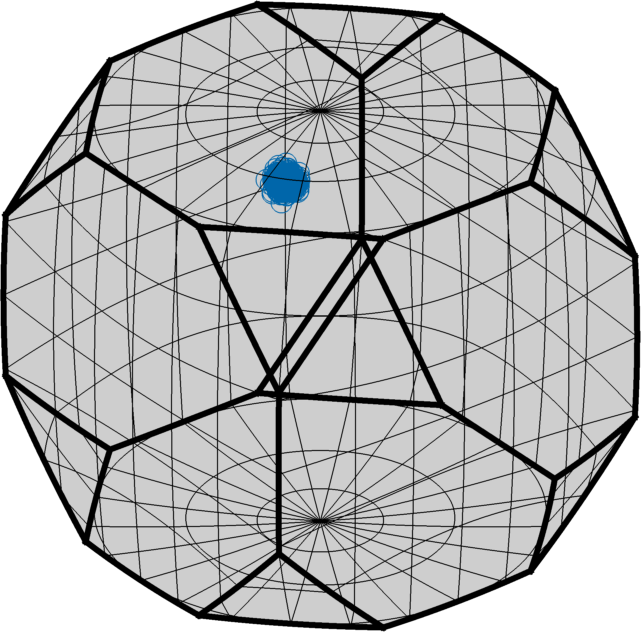
\includegraphics[width=4.5cm]{pic/oriParent}}
          \only<4>{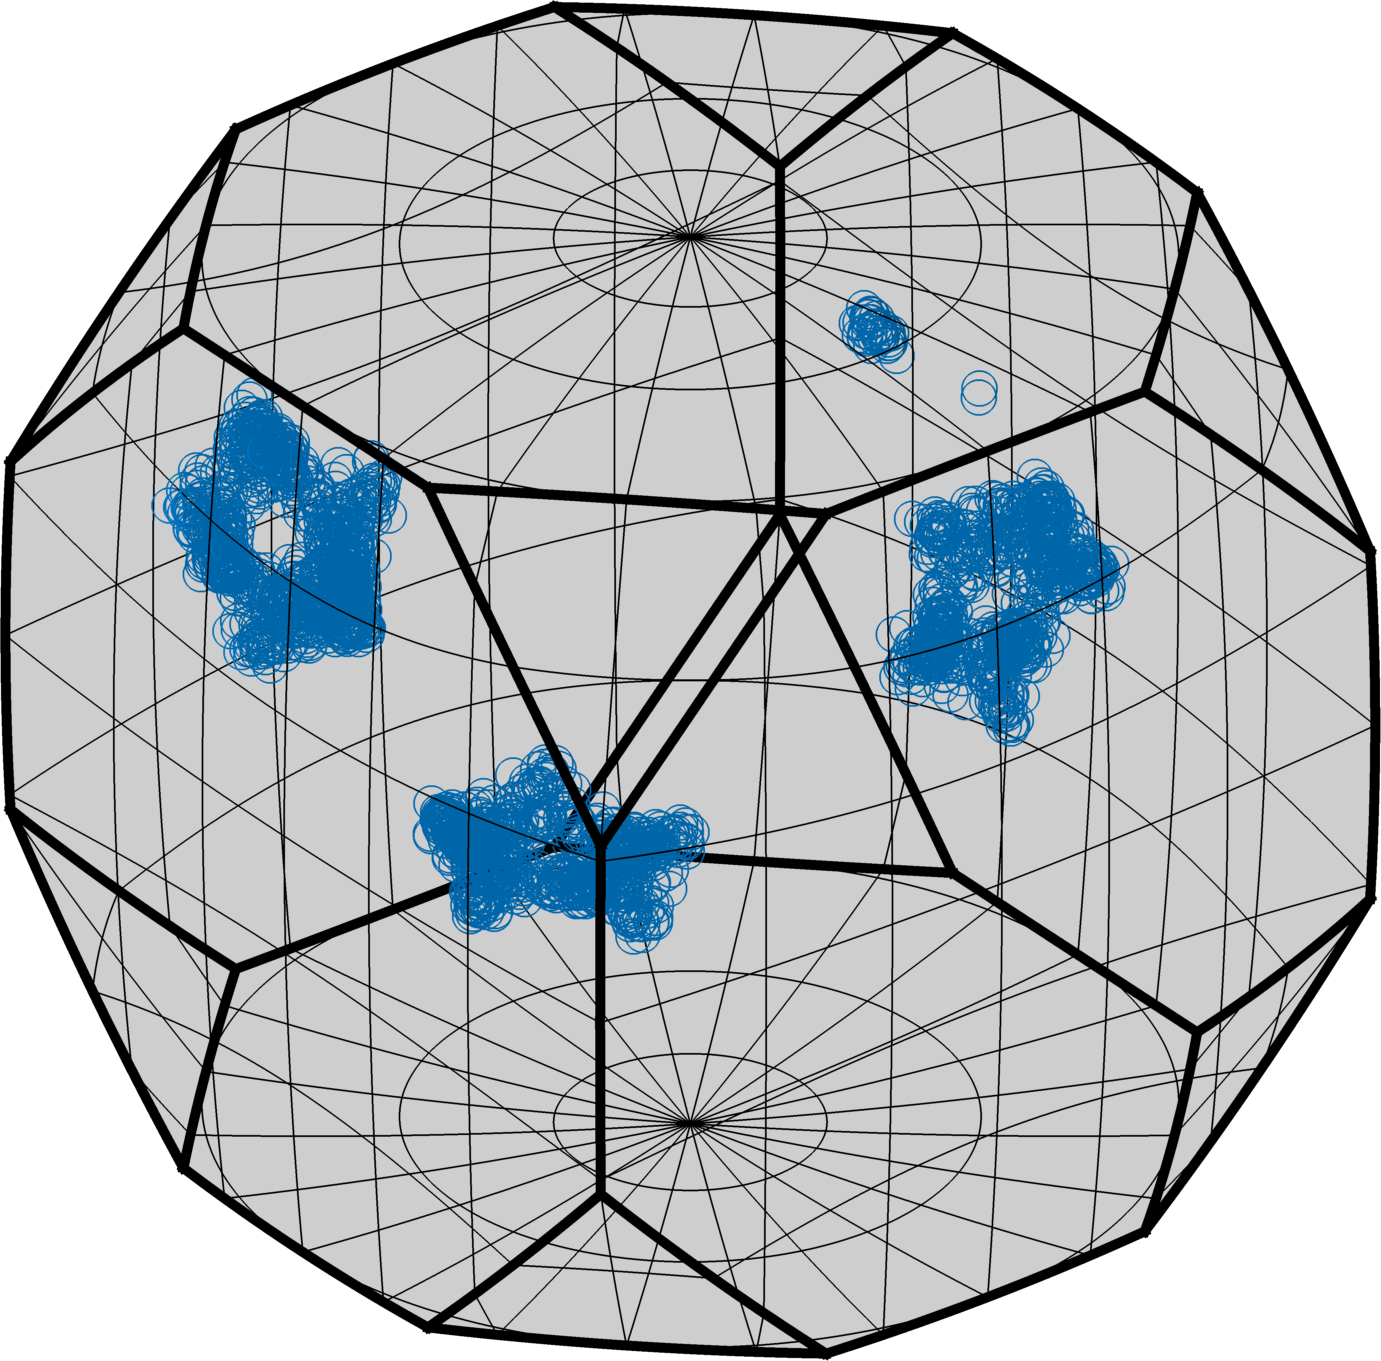
\includegraphics[width=4.5cm]{pic/oriChild}}
          \only<5>{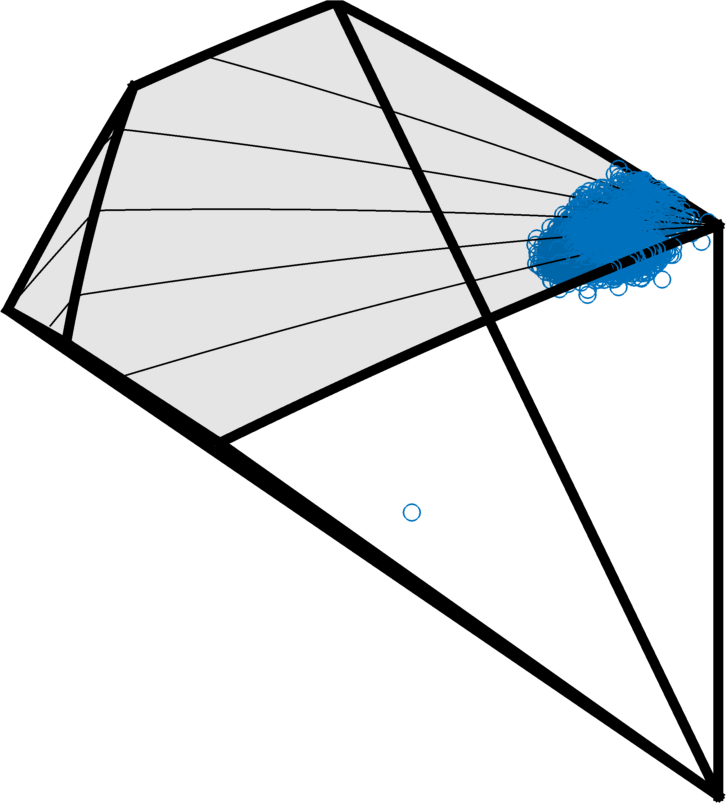
\includegraphics[width=4.5cm]{pic/moriScatterFull}}
        \end{center}
      \end{overlayarea}
    \end{column}
    \begin{column}{0.45\textwidth}
      \begin{overlayarea}{\textwidth}{0.9\textheight}
        \begin{center}
          \only<1>{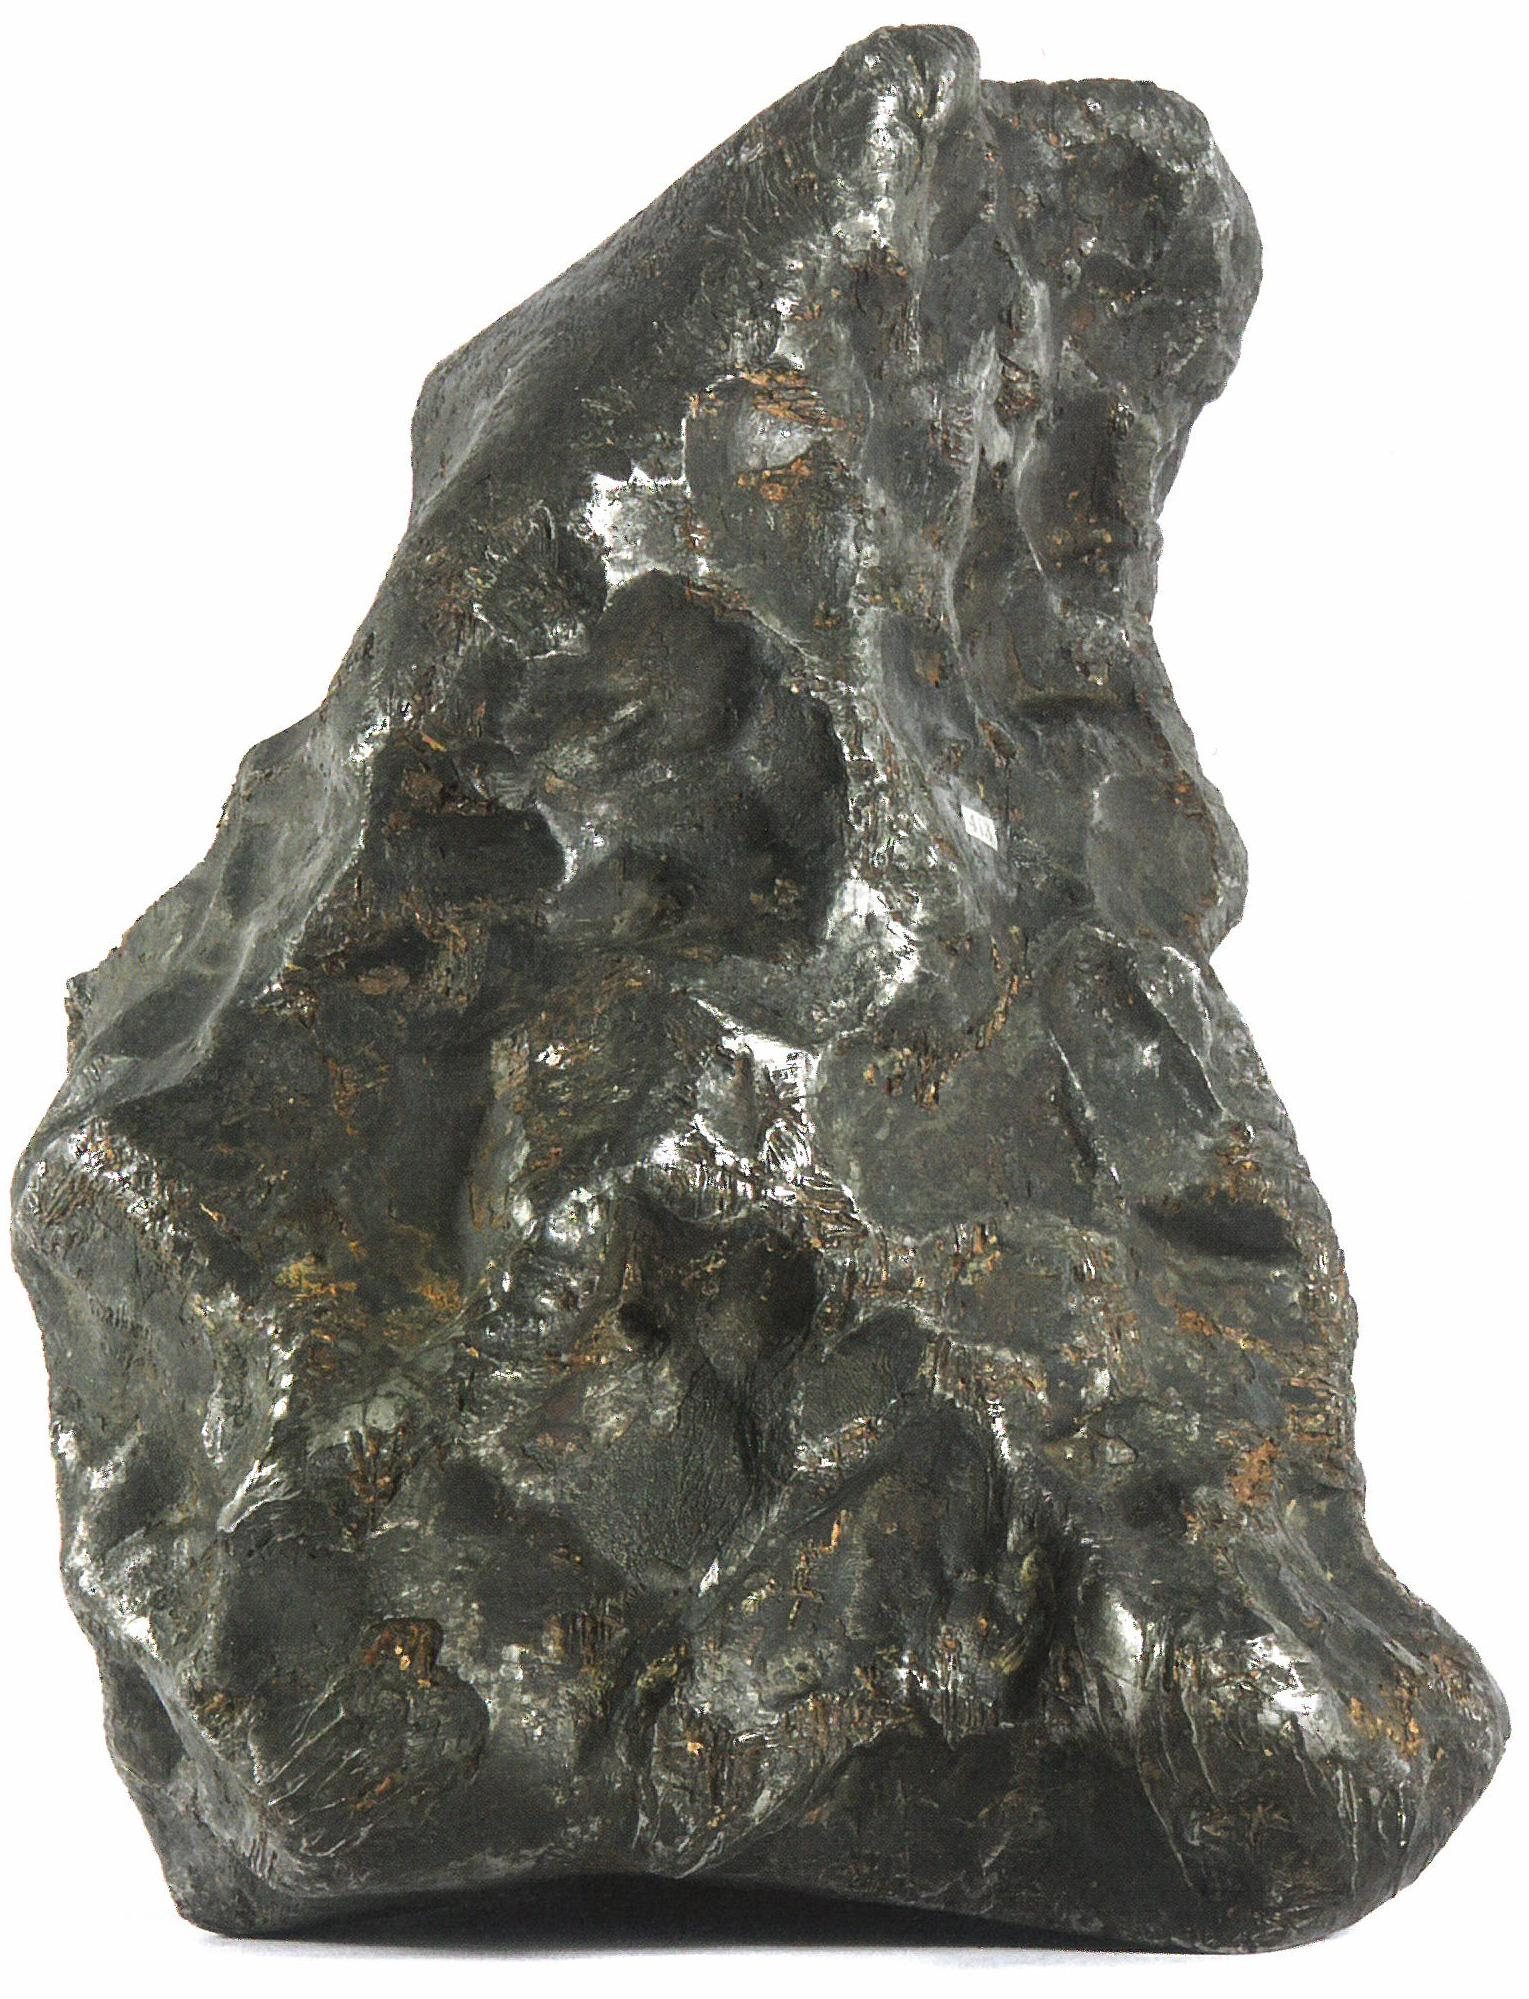
\includegraphics[width=0.8\textwidth]{pic/emslandMetereoit}\vspace{0.5cm}\
          }
          \only<2->{%
            \vspace{-1cm}%
            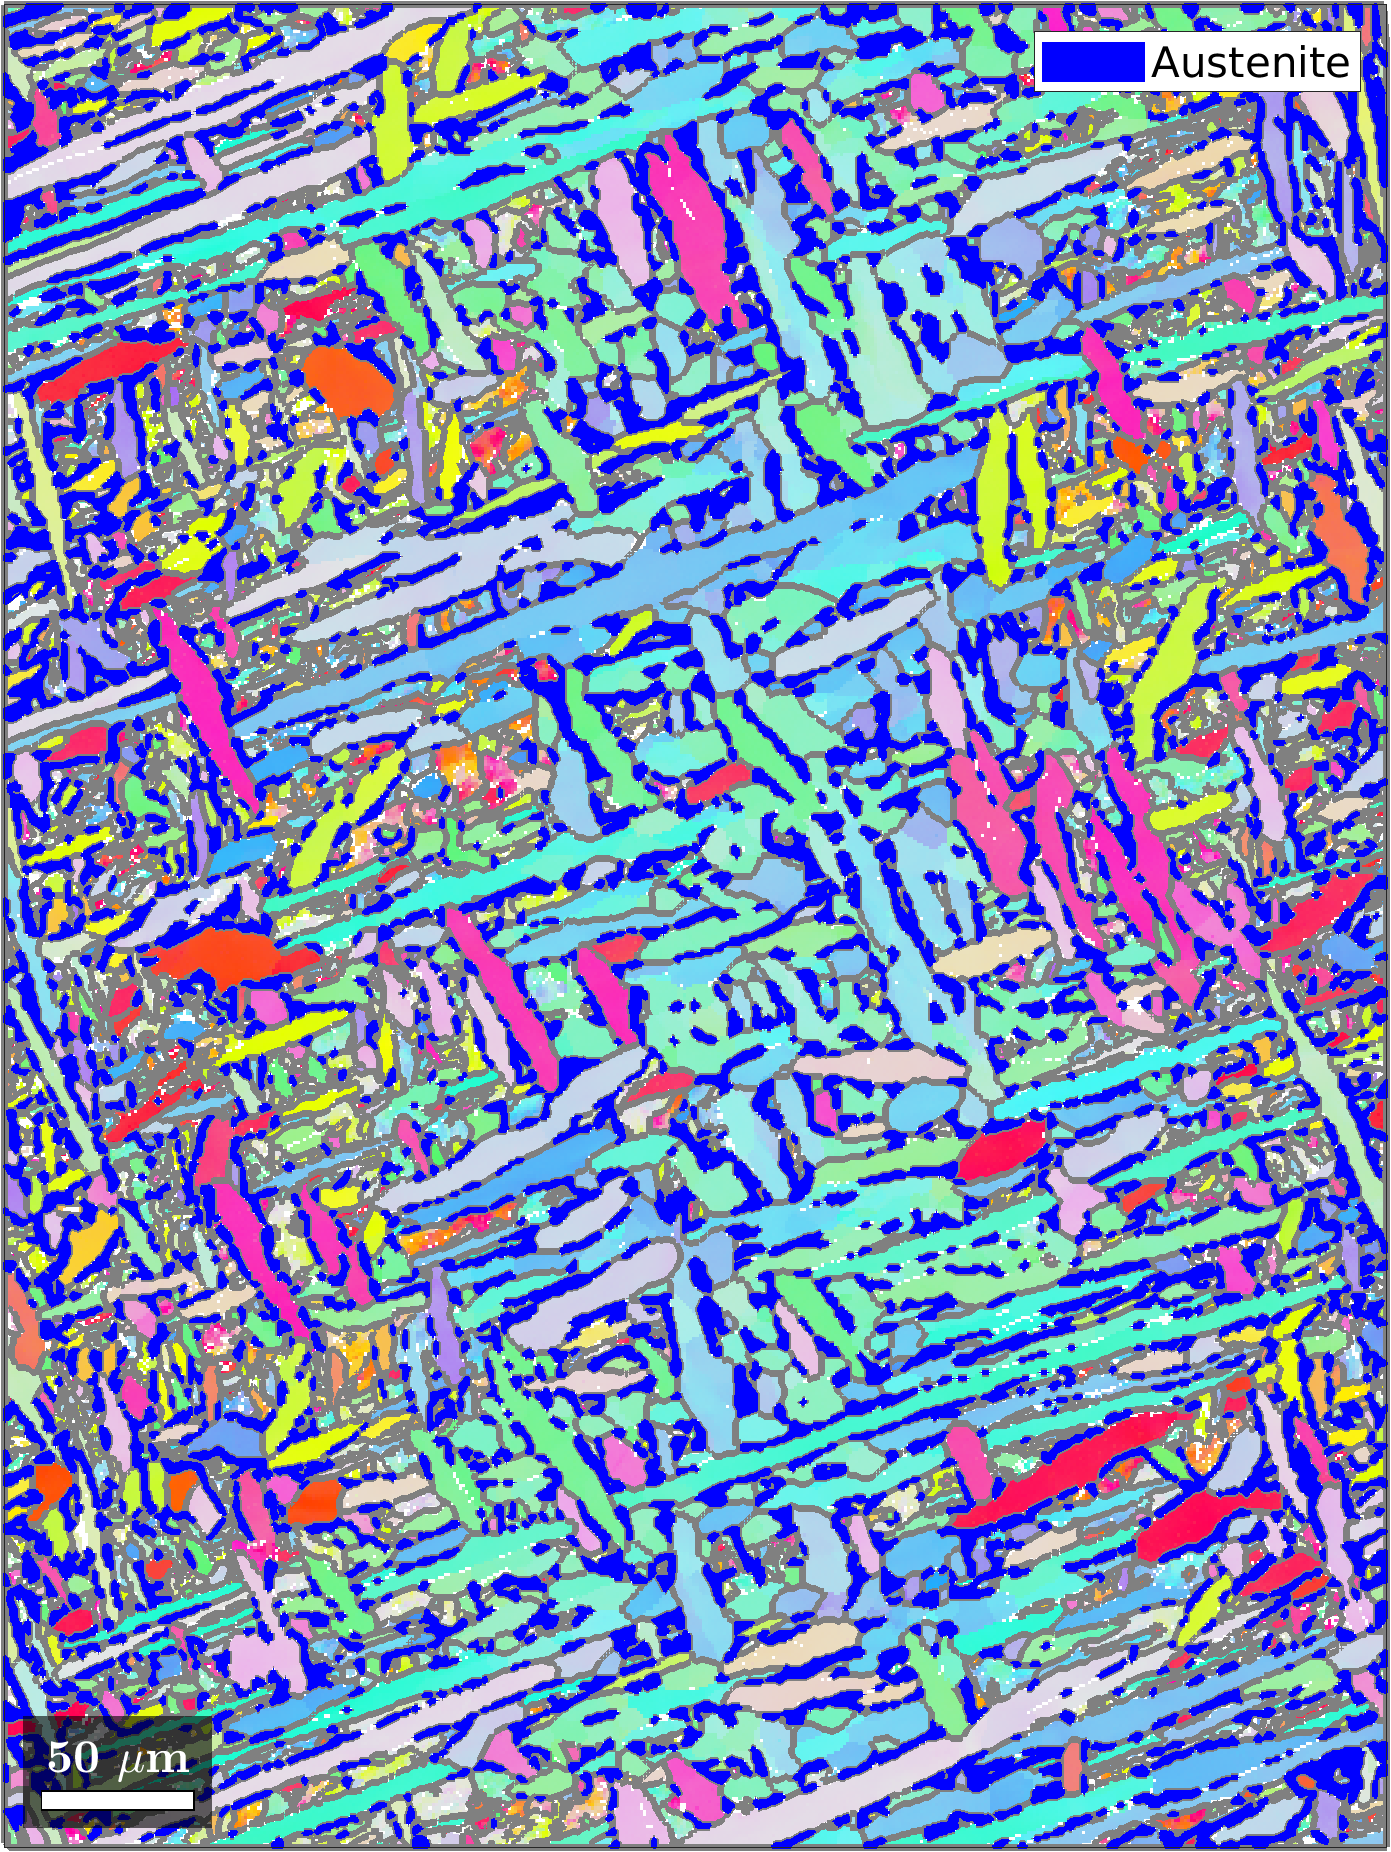
\includegraphics[height=0.95\textheight]{pic/mapFerrite}\vspace{0.5cm}\
          }
        \end{center}
      \end{overlayarea}
    \end{column}
  \end{columns}
\end{frame}

\section{Determination of the Parent to Child Orientation Relationship}



\begin{frame}[fragile]
  \frametitle{Theoretical Austenite $\rightarrow$ Ferrite Orientation Relationships}

\begin{center}
  \only<1>{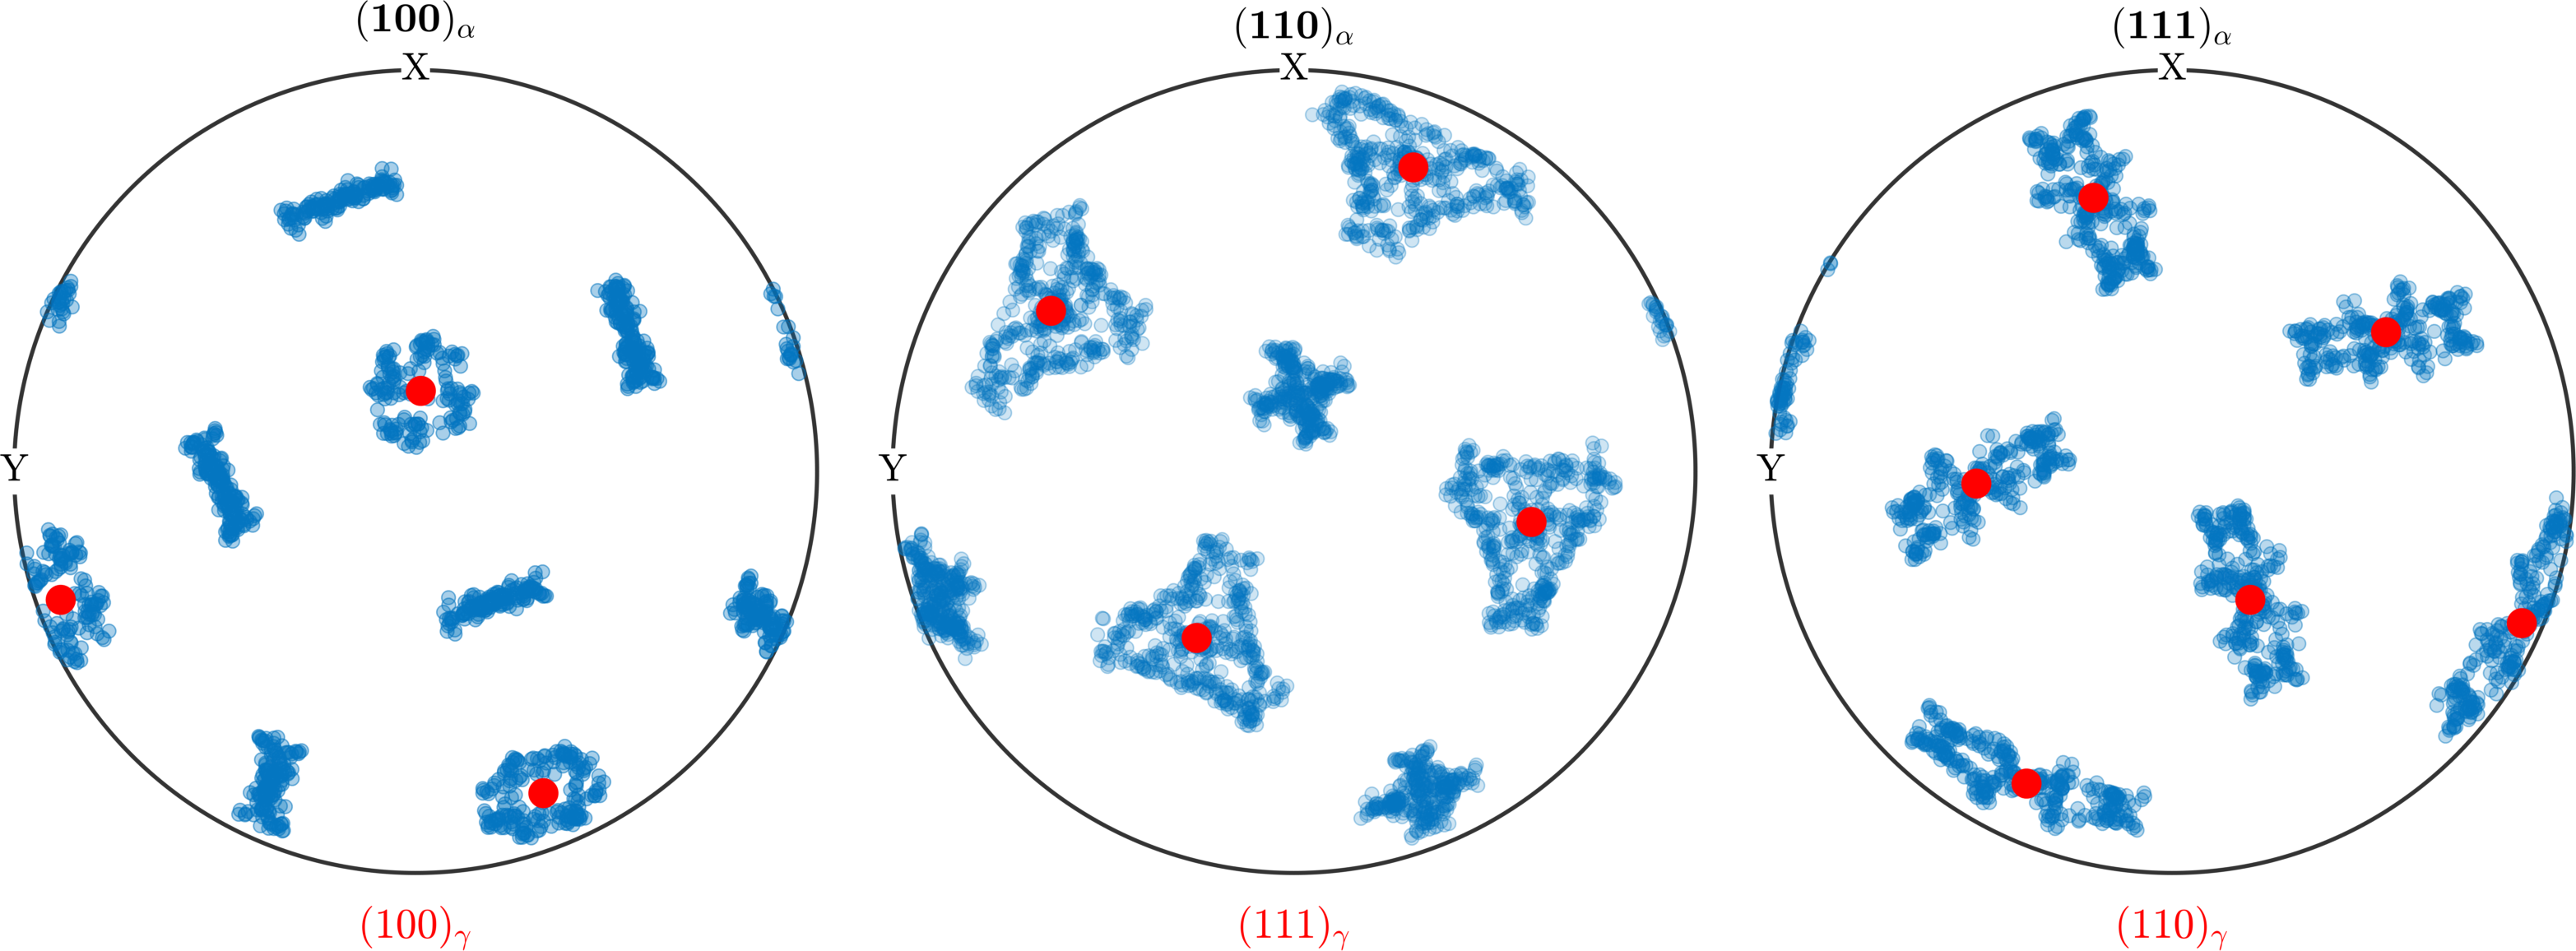
\includegraphics[width=0.925\textwidth]{pic/pfSuperposed.png}}
  \only<2>{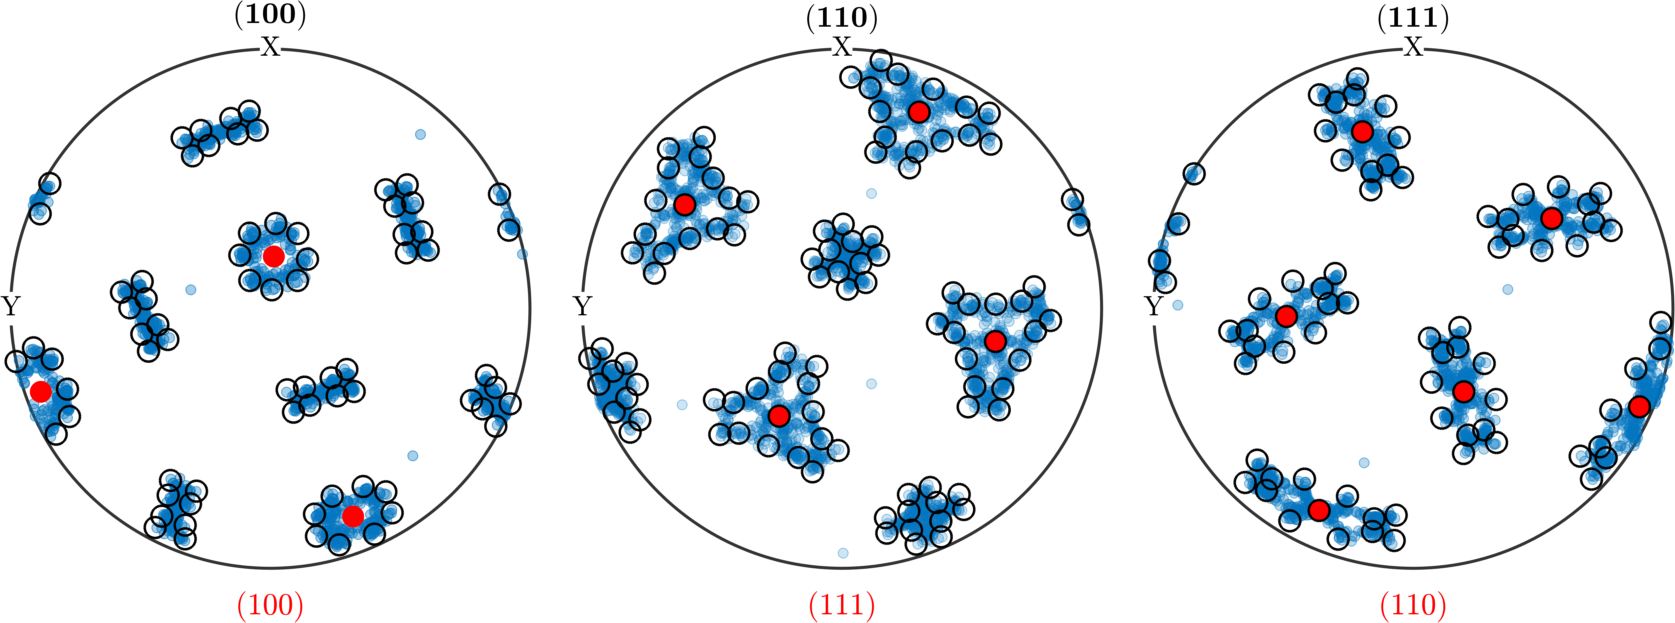
\includegraphics[width=0.925\textwidth]{pic/pfKS}}
  \only<3>{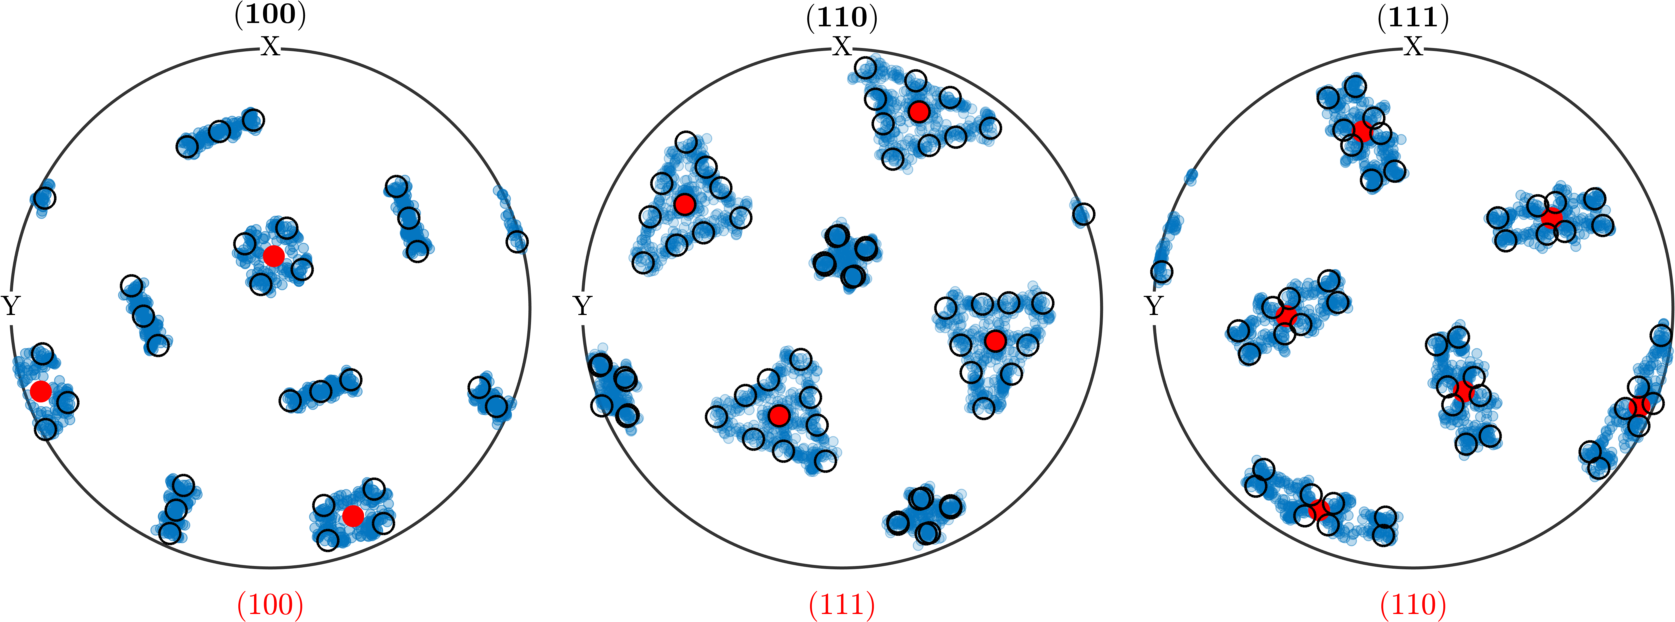
\includegraphics[width=0.925\textwidth]{pic/pfNW}}
  \only<4>{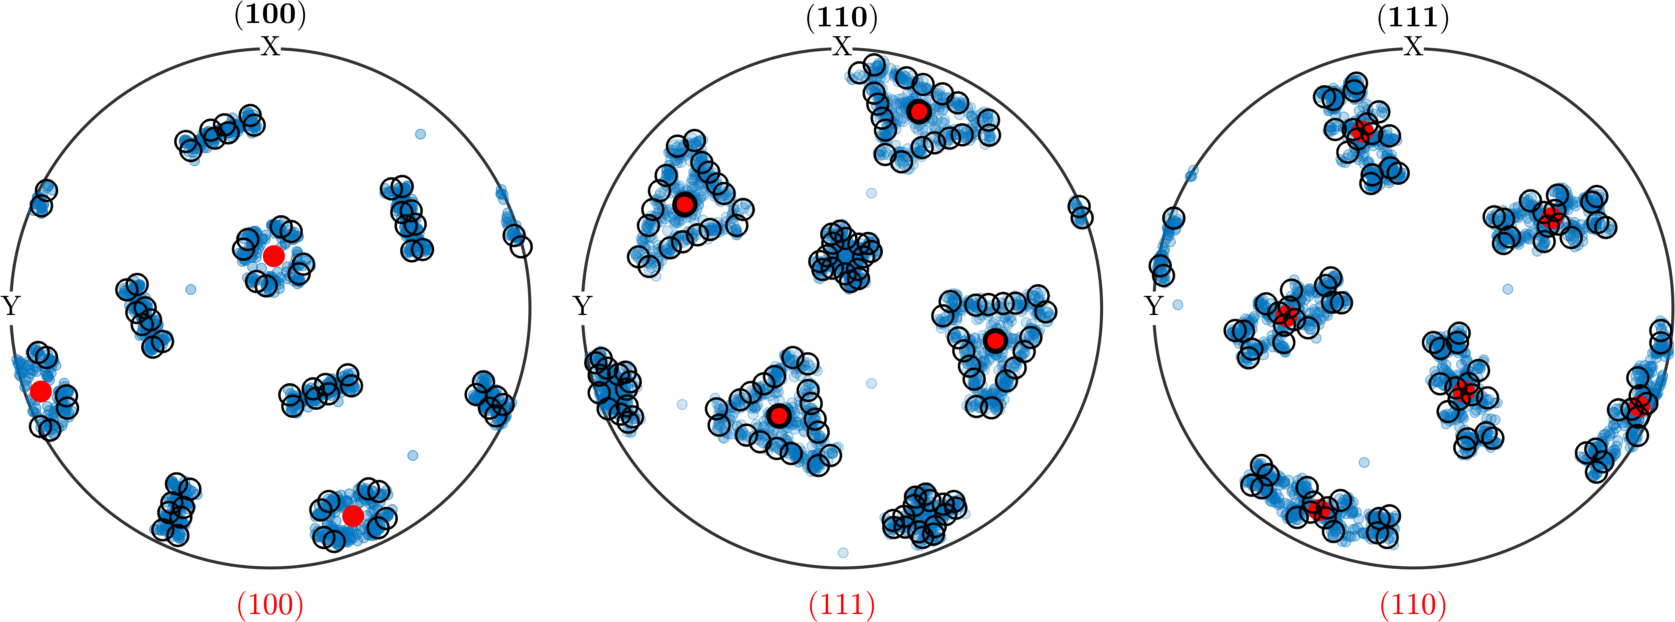
\includegraphics[width=0.925\textwidth]{pic/pfGT}}
  % \only<5>{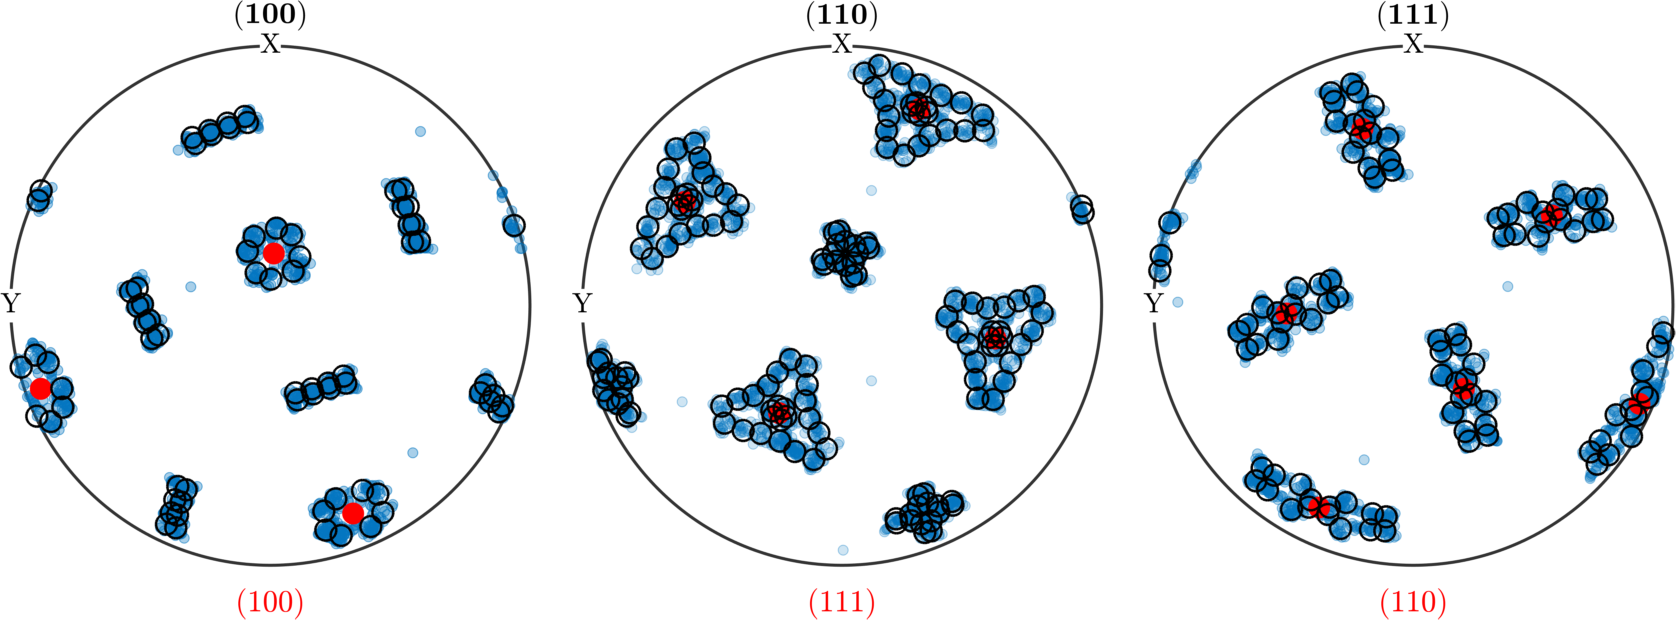
\includegraphics[width=\textwidth]{pic/pfMean}}
  % \only<6>{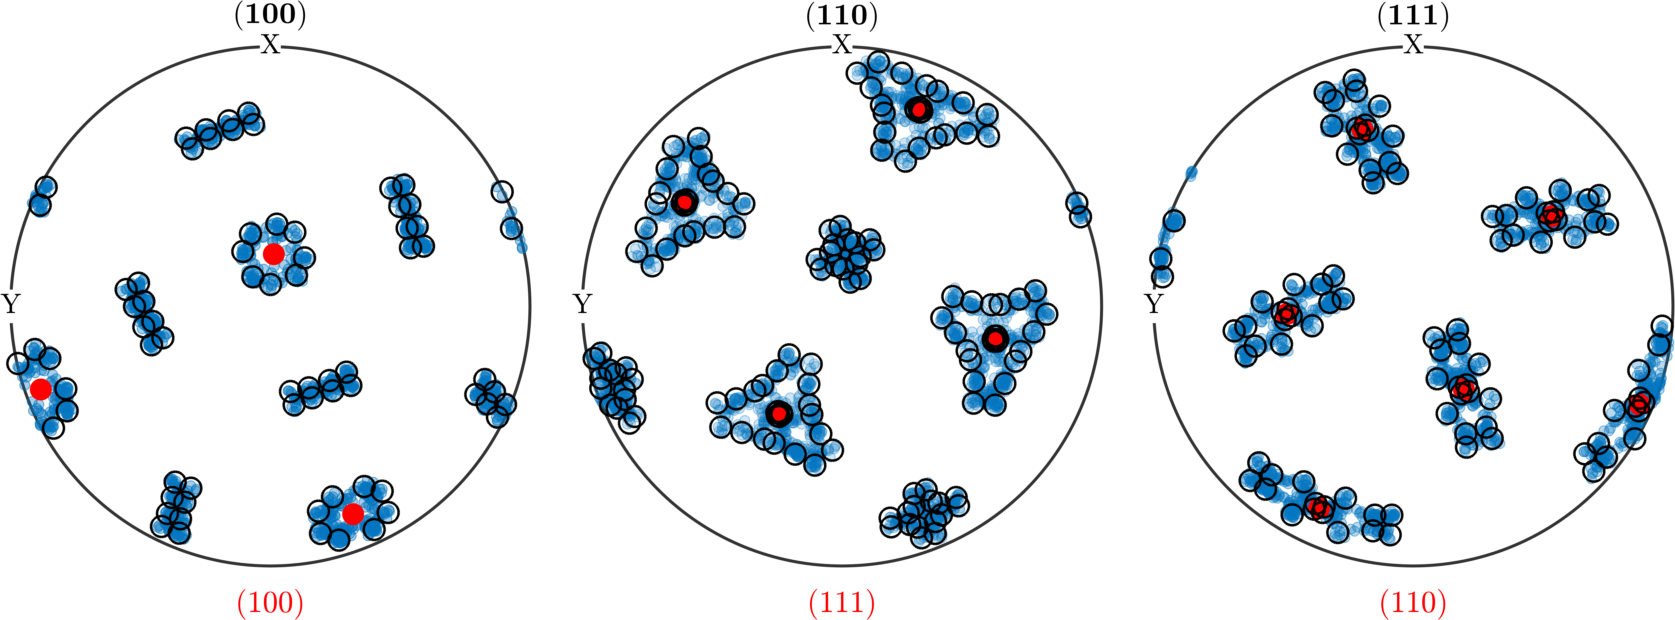
\includegraphics[width=\textwidth]{pic/pfMax}}
  % \only<7>{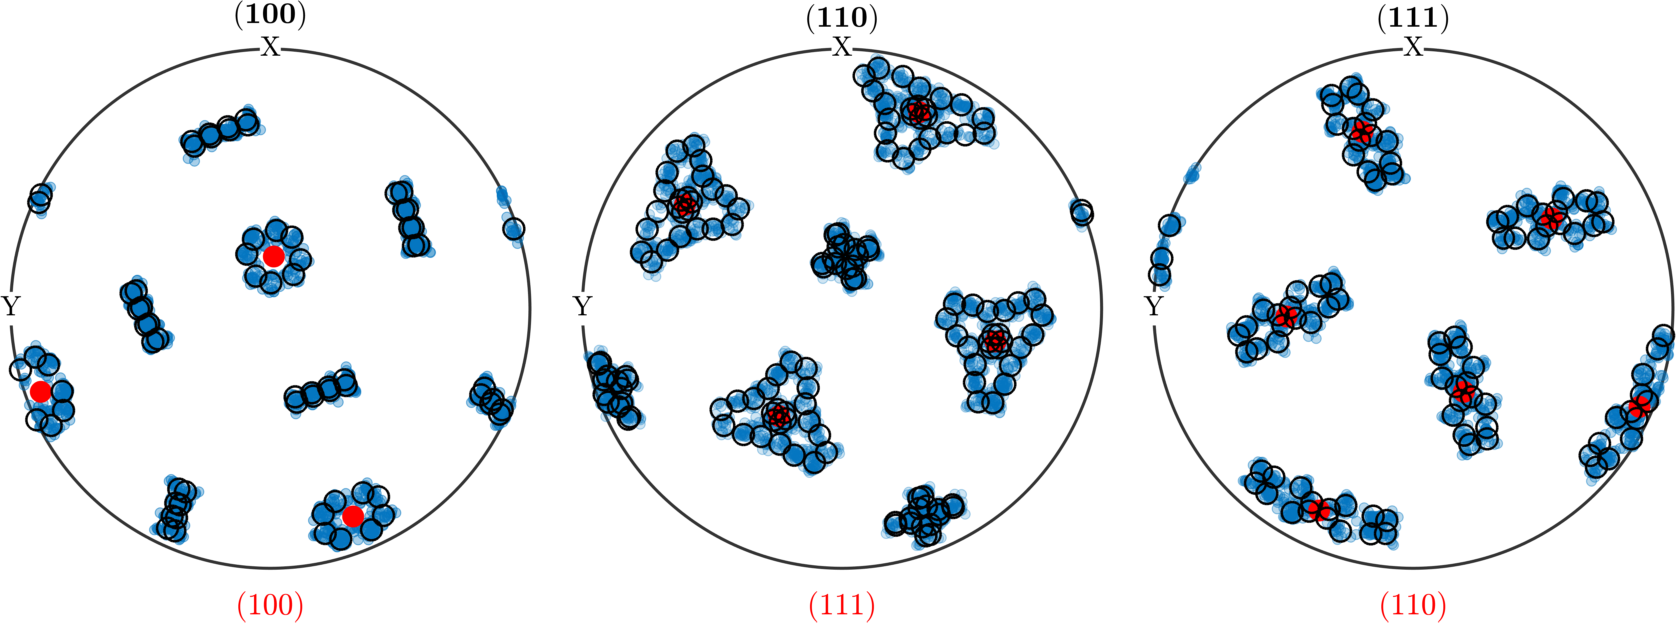
\includegraphics[width=\textwidth]{pic/pfIter}}
  % \only<8>{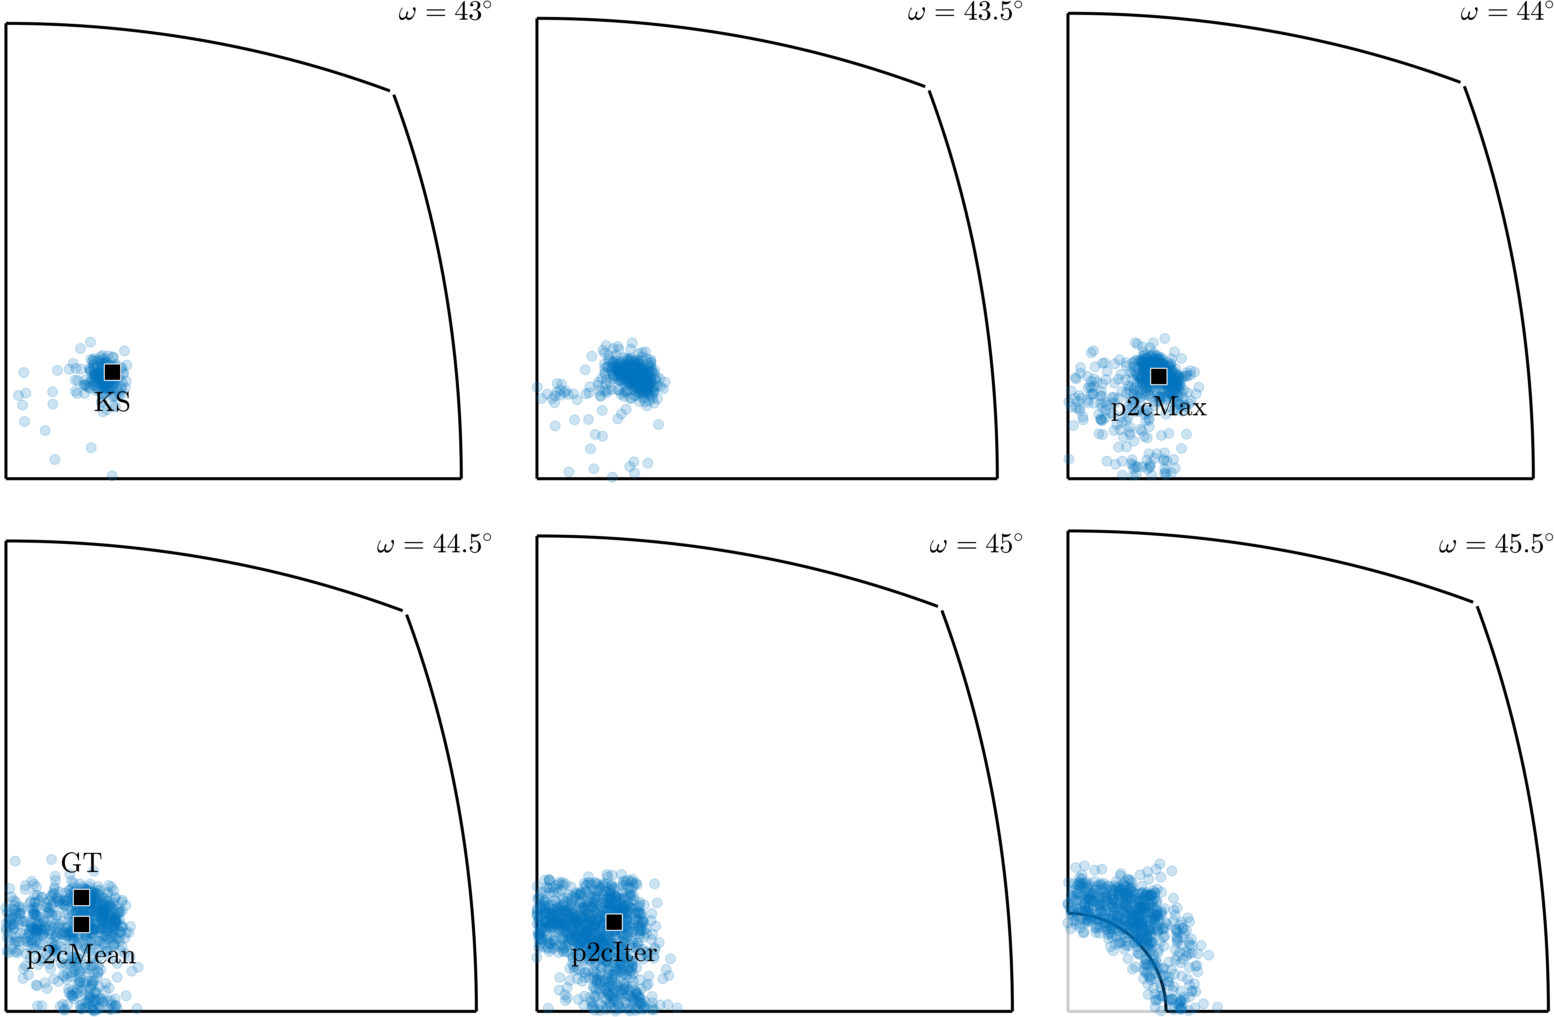
\includegraphics[width=0.8\textwidth]{pic/moriScatter}}
\end{center}

\vspace{-0.2cm}

  \begin{overlayarea}{\textwidth}{3cm}
    \begin{columns}[T,onlytextwidth]
      \begin{column}{0.59\textwidth}
        \begin{itemize}
        \item<1-> parent and child orientations in the meteorite
        \item<2-> Kurdjumov Sachs: $(111)_{\gamma} || (011)_{\alpha}$,
          $[\bar 101]_{\gamma} || [\bar 1 \bar 1 1]_{\alpha}$
        \item<3-> Nishiyama Wassermann:
          $(111)_{\gamma} || (011)_{\alpha}$,
          $[11\bar 2]_{\gamma} || [0\bar 1 1]_{\alpha}$
        \item<4-> Greninger Trojano
        \end{itemize}
      \end{column}
      \begin{column}{0.385\textwidth}
    \begin{onlyenv}<2>
\begin{lstlisting}[style=output]
p2c = misorientation (gamma -> alpha)
 
  Bunge Euler angles in degree
     phi1   Phi  phi2  Inv.
    335.8  10.5  65.8     0
\end{lstlisting}
    \end{onlyenv}
    \begin{onlyenv}<3>
\begin{lstlisting}[style=output]
p2c = misorientation (gamma -> alpha)
 
  Bunge Euler angles in degree
   phi1  Phi  phi2  Inv.
    180   99    45     0
\end{lstlisting}
    \end{onlyenv}
    \begin{onlyenv}<4>
\begin{lstlisting}[style=output]
p2c = misorientation (gamma -> alpha)
 
  Bunge Euler angles in degree
     phi1   Phi  phi2  Inv.
    172.5  46.6 177.3     0
\end{lstlisting}
    \end{onlyenv}
  \end{column}
\end{columns}
  \begin{onlyenv}<2>
\begin{lstlisting}[style=input]
gamma_111 = Miller(1,1,1,csGamma,'hkl')
p2c = orientation.map( gamma_111, alpha_100, gamma_101, alpha_111)
\end{lstlisting}
    \end{onlyenv}
    \begin{onlyenv}<3>
\begin{lstlisting}[style=input]
p2c = orientation.NishiyamaWassermann(csGamma,csAlpha)
\end{lstlisting}
    \end{onlyenv}
    \begin{onlyenv}<4>
\begin{lstlisting}[style=input]
p2c = orientation.GreningerTrojano(csGamma,csAlpha)
\end{lstlisting}
    \end{onlyenv}
  \end{overlayarea}
\end{frame}




\begin{frame}[fragile]
  \frametitle{Experimental Austenite $\rightarrow$ Ferrite Orientation Relationships}

  \begin{center}
    \only<1>{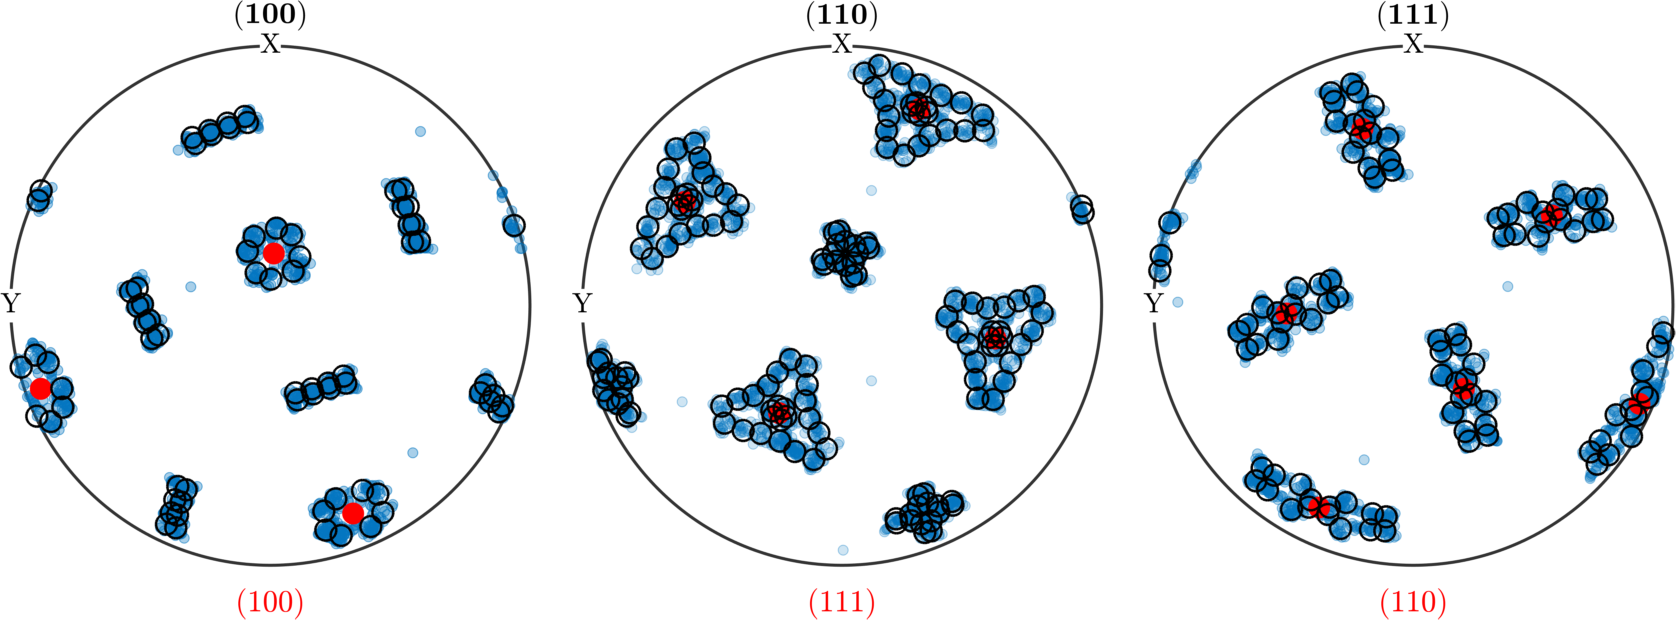
\includegraphics[width=0.925\textwidth]{pic/pfMean}}
    \only<2>{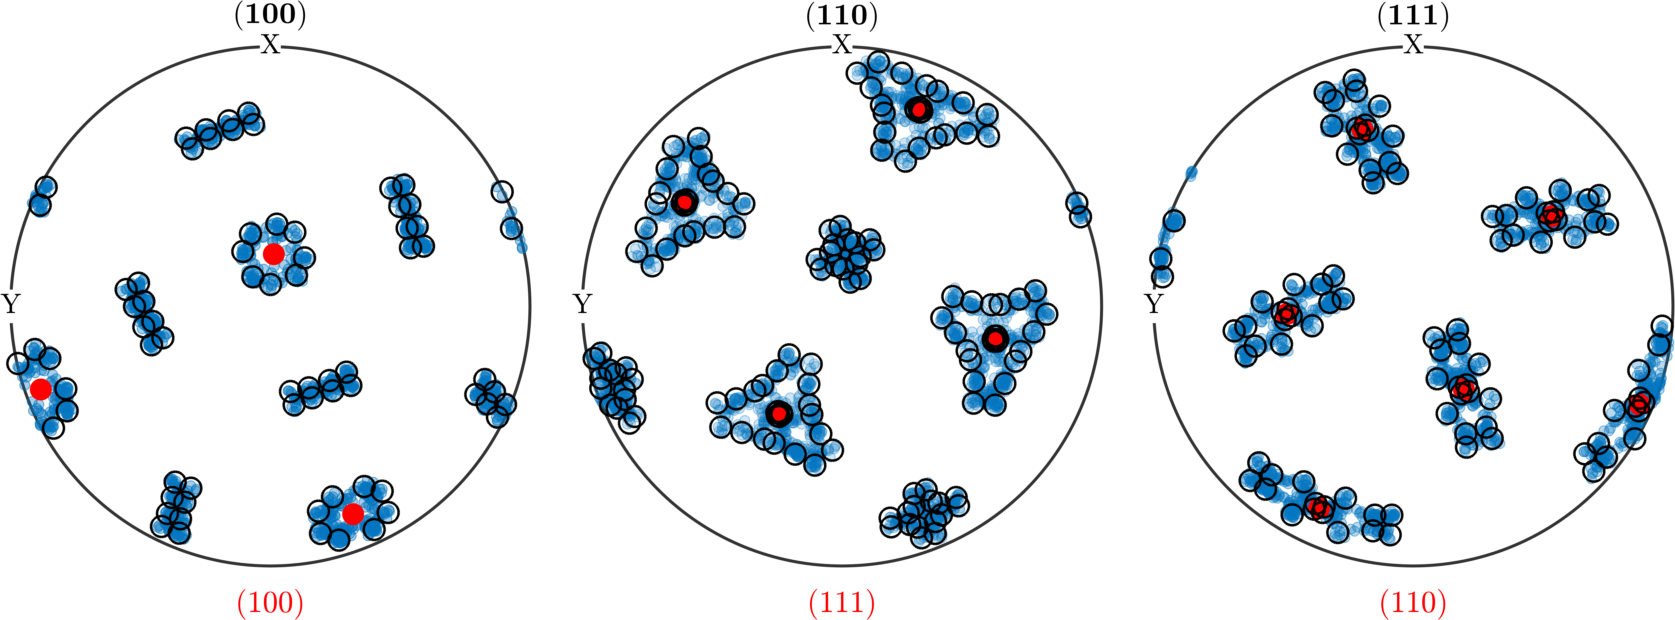
\includegraphics[width=0.925\textwidth]{pic/pfMax}}
    \only<3-4>{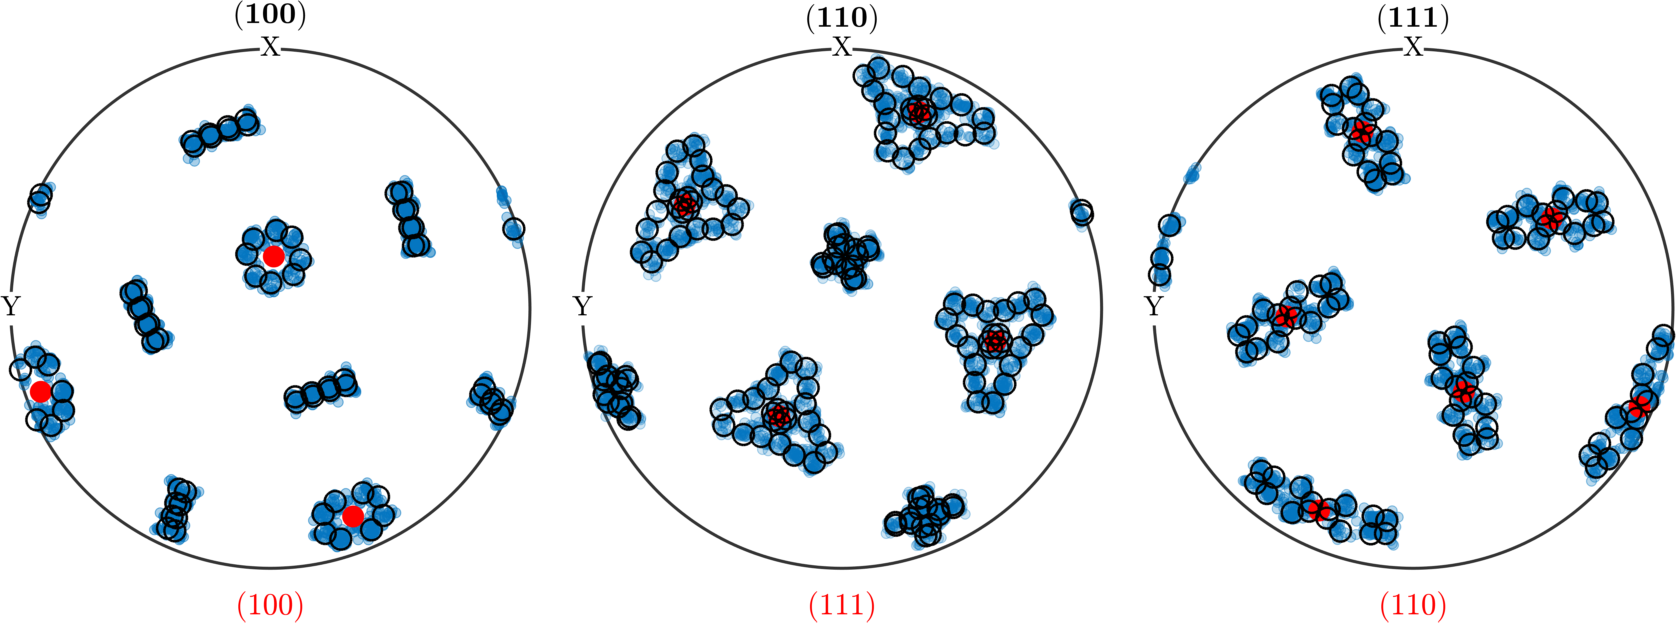
\includegraphics[width=0.925\textwidth]{pic/pfIter}}
    \only<5>{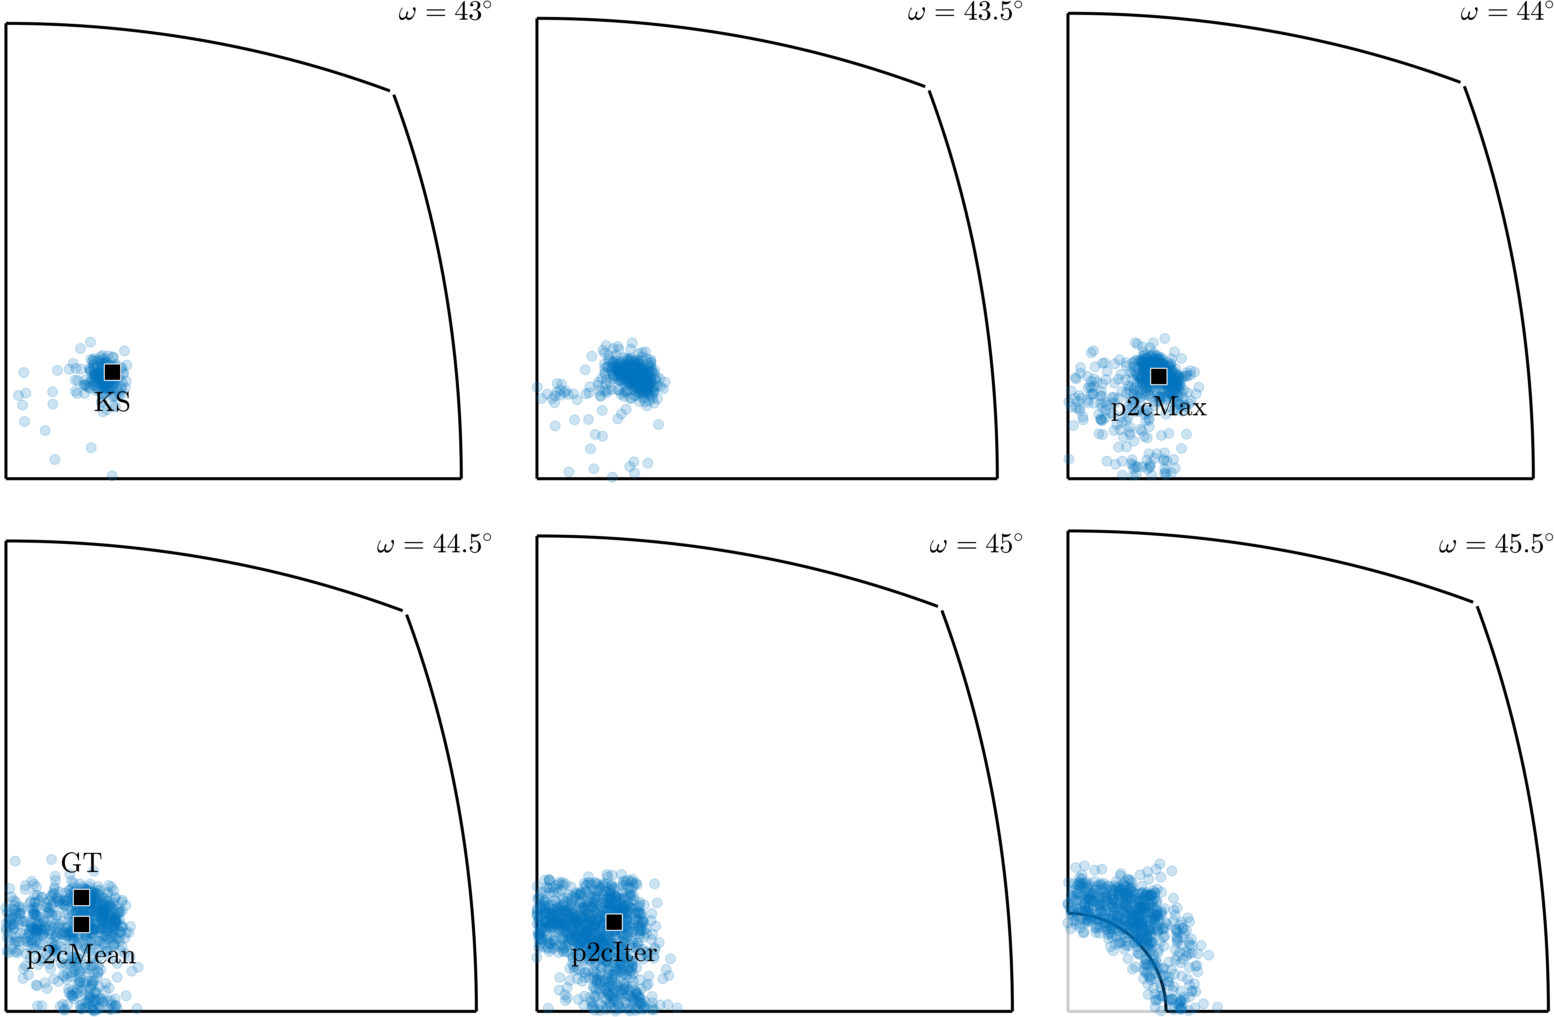
\includegraphics[width=0.825\textwidth]{pic/moriScatter.png}}
  \end{center}
  \begin{overlayarea}{\textwidth}{3cm}
    \begin{itemize}
    \item<1-4> average parent to child misorientation%: \lstinline{p2cMean = mean( inv(oriChild) * oriP )}
      \uncover<2-4>{\paritem maximum of misorientation distribution function}        
    \item<3-4> maximize fit to all child to child misorientations
      \uncover<4>{\paritem iterative method of T. Nyyssönen}
    \end{itemize}
        \begin{onlyenv}<1>
\begin{lstlisting}[style=input]
mori = grains.boundary('gamma','alpha').misorientation
p2c  = mean(mori)
\end{lstlisting}
        \end{onlyenv}
        \begin{onlyenv}<2>
\begin{lstlisting}[style=input]
mdf = calcDensity(mori)
[~,p2c] = max(mdf)
\end{lstlisting}
        \end{onlyenv}
        \begin{onlyenv}<3-4>
\begin{lstlisting}[style=input]
mori = grains.boundary('alpha','alpha').misorientation
p2c  = calcParent2Child(mori)
\end{lstlisting}
        \end{onlyenv}
      \end{overlayarea}


\end{frame}


\begin{frame}[fragile]
  \frametitle{Parent and Child Variants}

  \begin{overlayarea}{\textwidth}{0.85\textheight}
    \begin{columns}[T,onlytextwidth]
      \begin{column}{0.58\textwidth}
        \begin{block}{}
          \begin{itemize}
          \item $\mathtt{ori_{P}}$ - parent orientation
            \paritem $\mathtt{ori_{C}}$ - child orientation
          \item $\mathtt{sym_{P}}$ - parent symmetry \hspace{1pt}
            \paritem $\mathtt{sym_{C}}$ - child symmetry
          \item $\mathtt{p2c}$ - parent to child misorientation
          \end{itemize}
        \end{block}

        % \vspace{-0.5cm}


        \structure{child variants:}
        $\mathtt{ori_{P}} = \mathtt{ori_{C}} \cdot \mathtt{sym_{C}} \cdot
        \mathtt{p2c}$

        \medskip
        
        \structure{parent variants:}
        $\mathtt{ori_{C}} = \mathtt{ori_{P}} \cdot \mathtt{sym_{P}} \cdot
        \mathtt{inv}(\mathtt{p2c})$

       
        \begin{onlyenv}<2->
\begin{lstlisting}[style=input]
cv = variants(p2c,ori_p)
pv = variants(p2c,ori_c)
\end{lstlisting}
        \end{onlyenv}
        \begin{onlyenv}<2>
          \vspace{-0.3cm}
\begin{lstlisting}[style=output]
cv = misorientation (Austenite -> Ferrite, bcc)
  size: 1 x 24

pv = misorientation (Ferrite, bcc -> Austenite)
  size: 1 x 24
 \end{lstlisting}
      \end{onlyenv}
      

      \bigskip

      \begin{onlyenv}<3->
        \structure{Child to Child Misorientation:}
        \vspace{-0.2cm}
\begin{lstlisting}[style=input]
c2c = p2c * sym_P * inv(p2c)
c2c = variants(p2c,'child') * inv(p2c)
\end{lstlisting}
      \end{onlyenv}
        \begin{onlyenv}<3>
          \vspace{-0.3cm}
\begin{lstlisting}[style=output]
c2c = misorientation (Ferrite, bcc -> Ferrite, bcc)
  size: 1 x 24
 \end{lstlisting}
        \end{onlyenv}
        
      \bigskip

      \begin{onlyenv}<4->
        \structure{Detect Child to Child Grain Boundaries:}
        \vspace{-0.2cm}
\begin{lstlisting}[style=input]
omega = angle_outer(gB.misorientation,c2c)
pg = merge(grains, gB(omega < 5*degree) )
\end{lstlisting}
      \end{onlyenv}
    \end{column}
    \begin{column}{0.4\textwidth}
      \only<1>{
        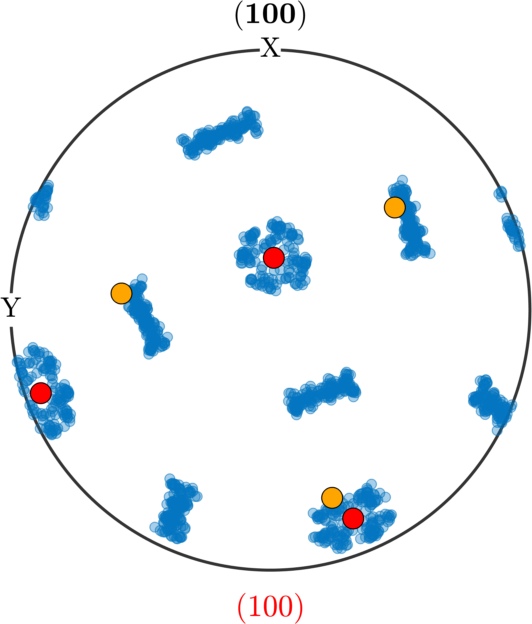
\includegraphics[width=\textwidth]{pic/pfSingleVariant1}}%
      \only<2>{%
        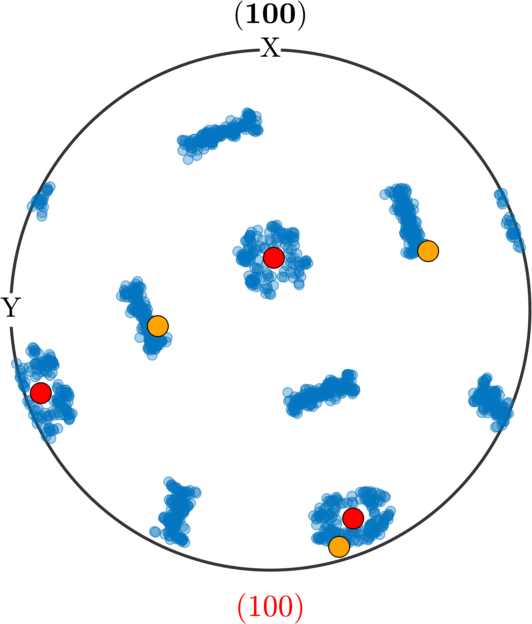
\includegraphics[width=\textwidth]{pic/pfSingleVariant2}}%
      \only<3>{%
        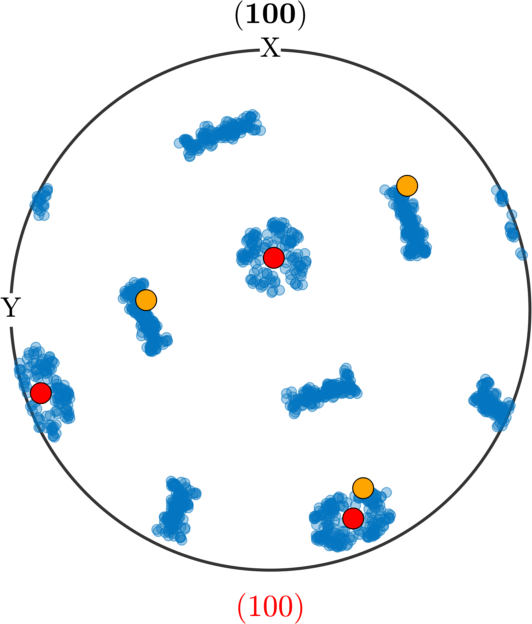
\includegraphics[width=\textwidth]{pic/pfSingleVariant3}}
      \only<4>{%
        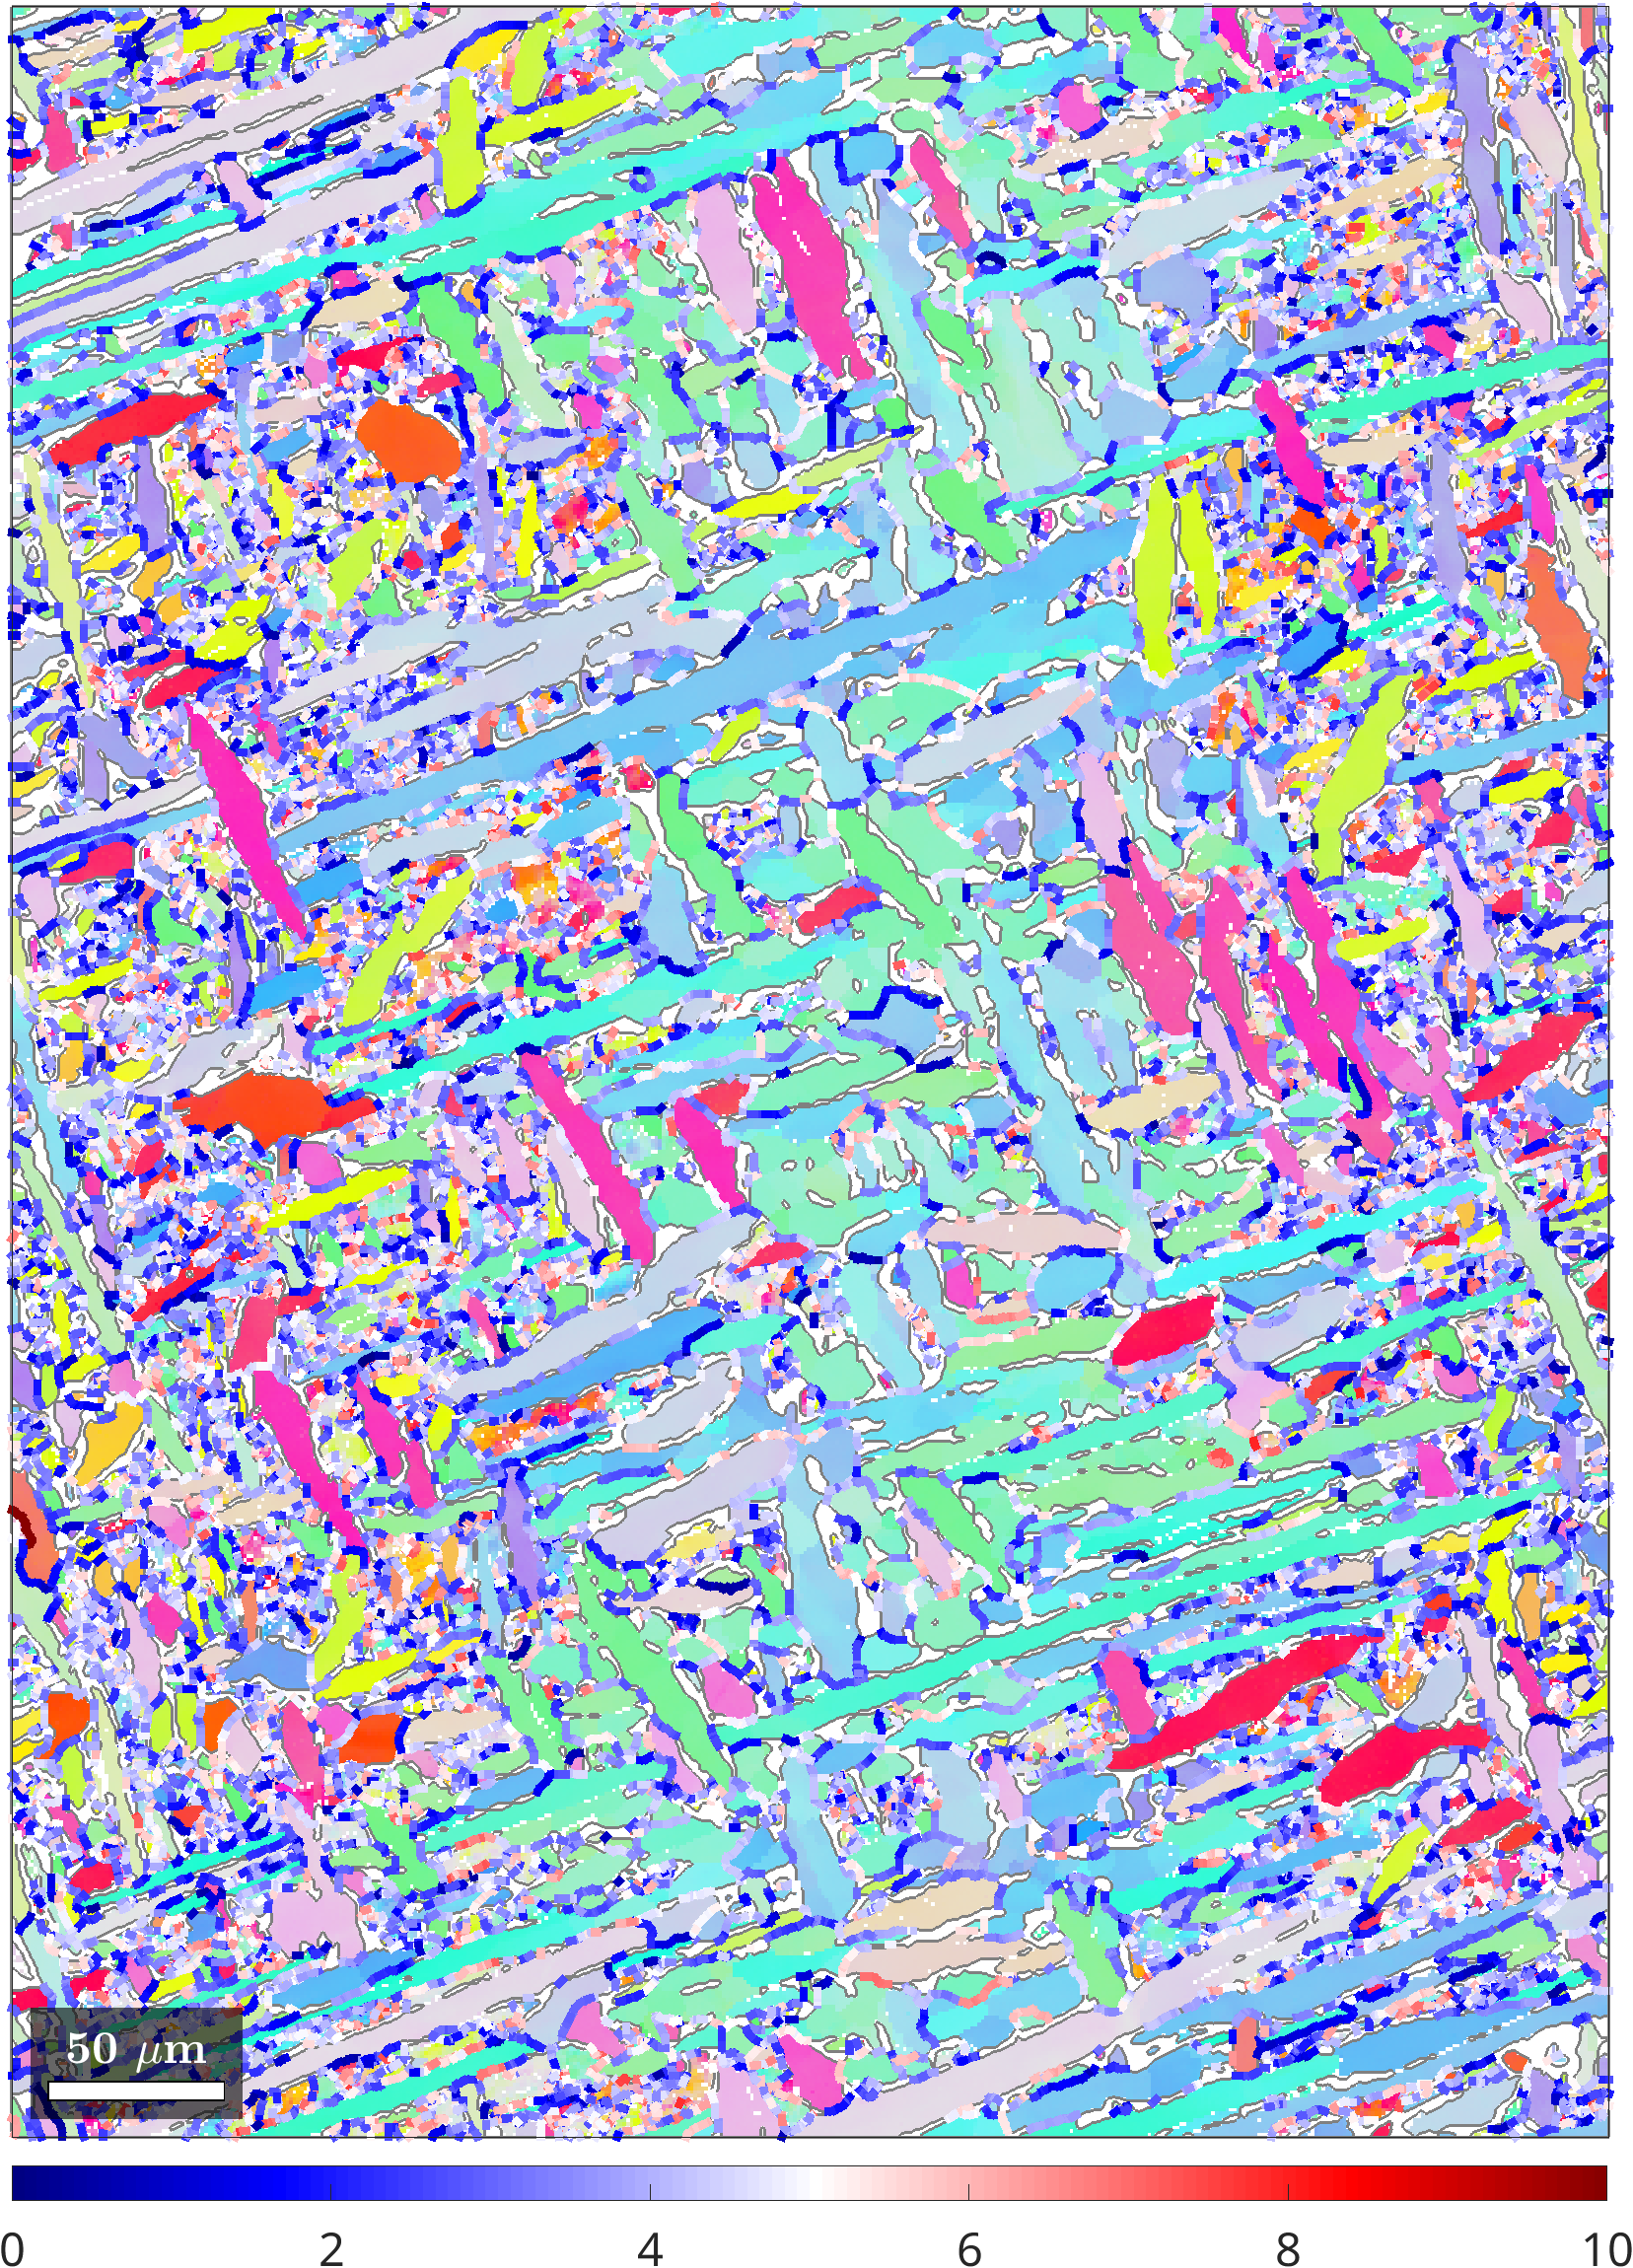
\includegraphics[width=\textwidth]{pic/mapFerriteBoundaries}}%
    \end{column}
  \end{columns}
\end{overlayarea}
\end{frame}


\begin{frame}

  \frametitle{A two-stage transformation microstructure}

    \begin{overlayarea}{\textwidth}{0.85\textheight}

  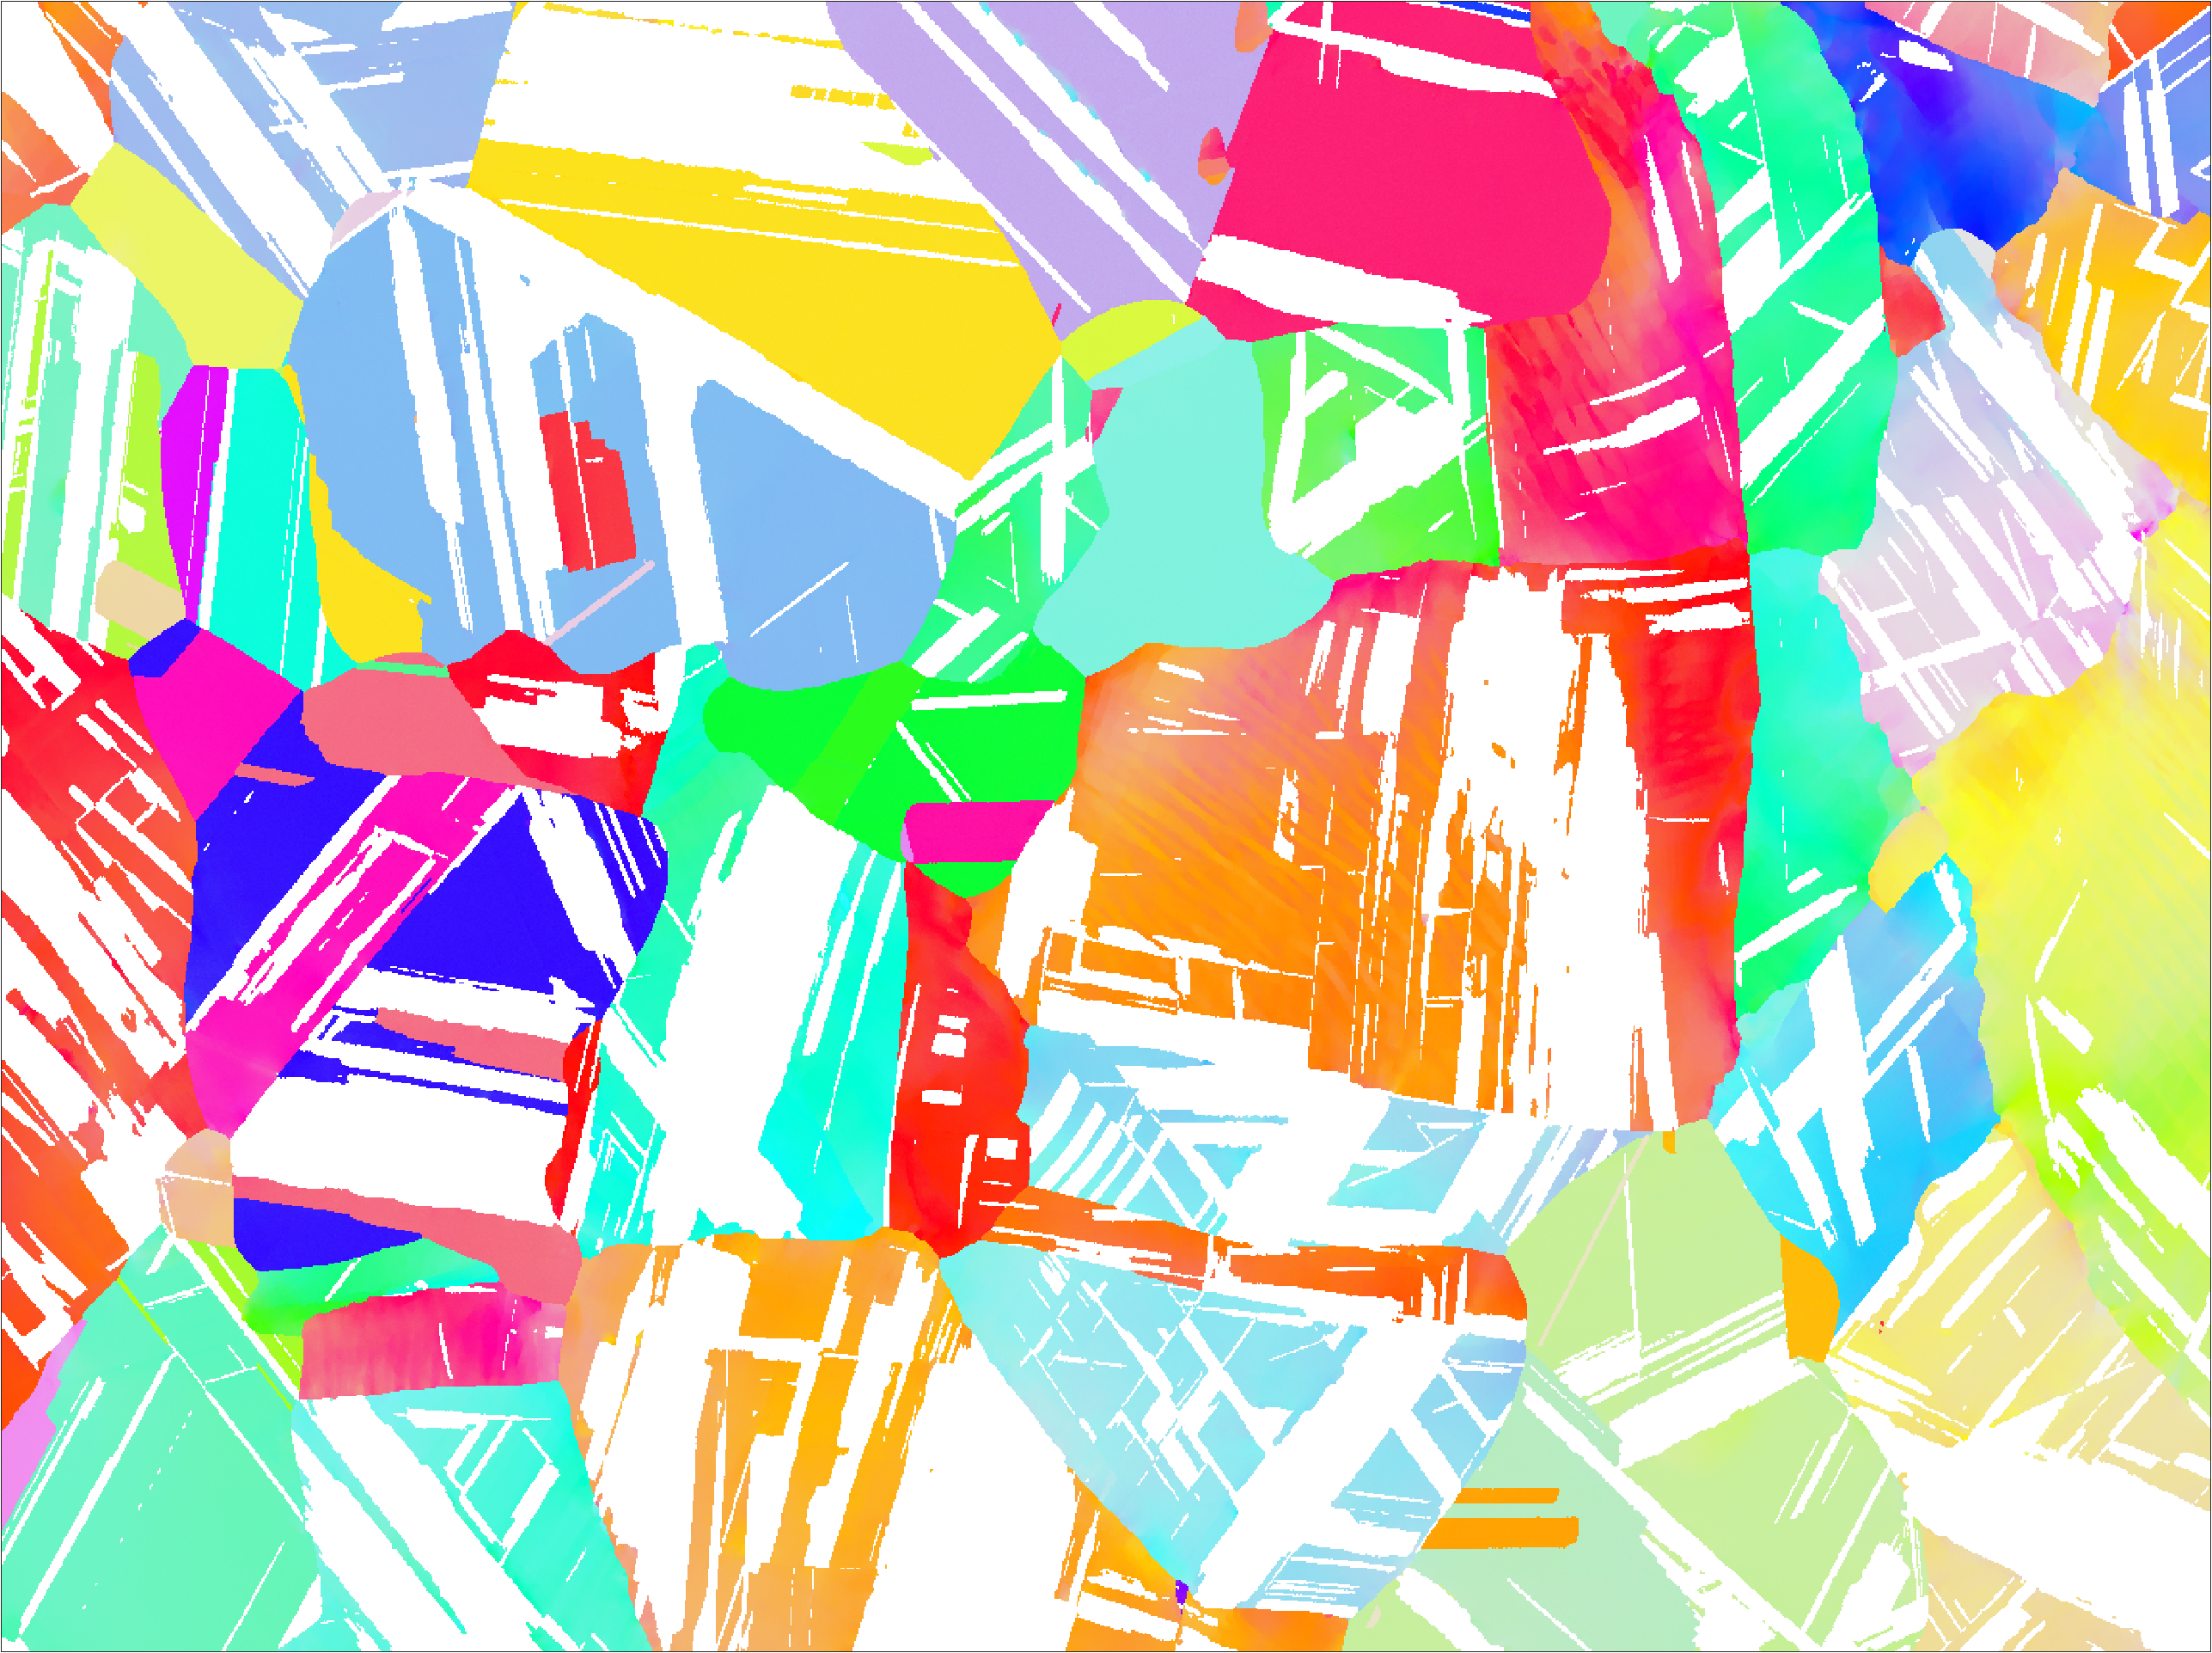
\includegraphics[width=0.3\textwidth]{pic/gammaRaw}
  \quad
  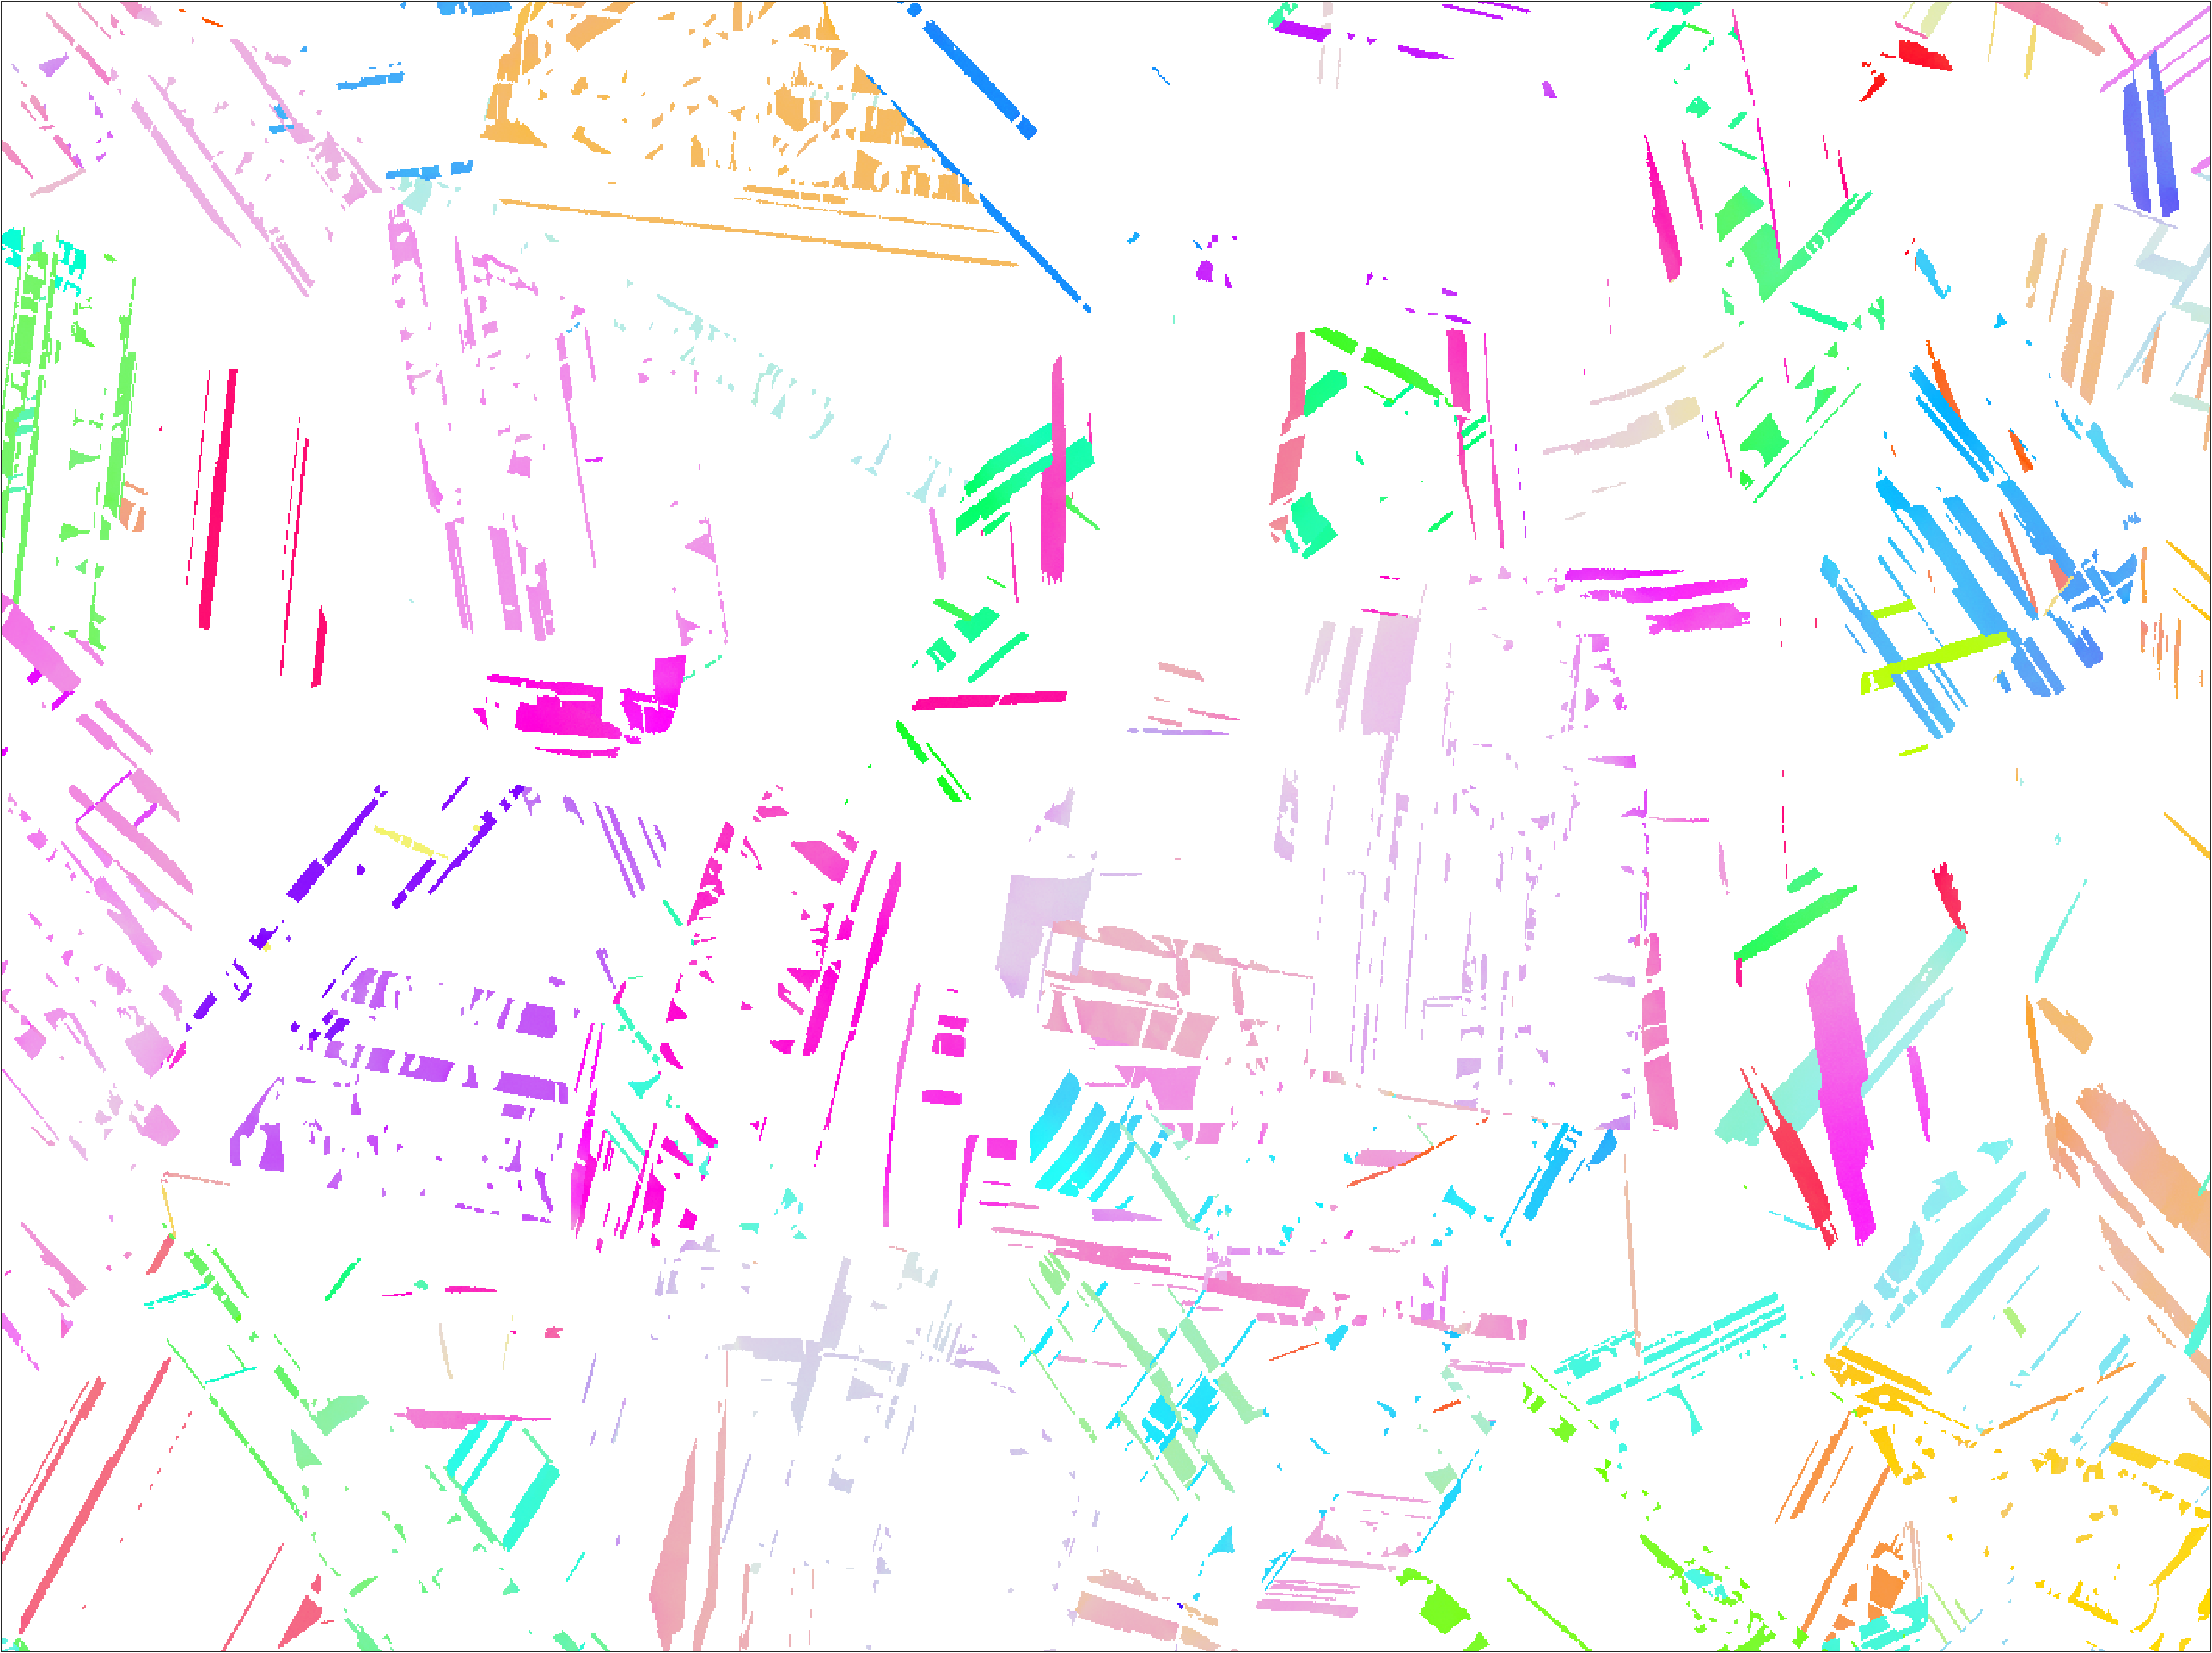
\includegraphics[width=0.3\textwidth]{pic/EpsRaw}
  \quad
  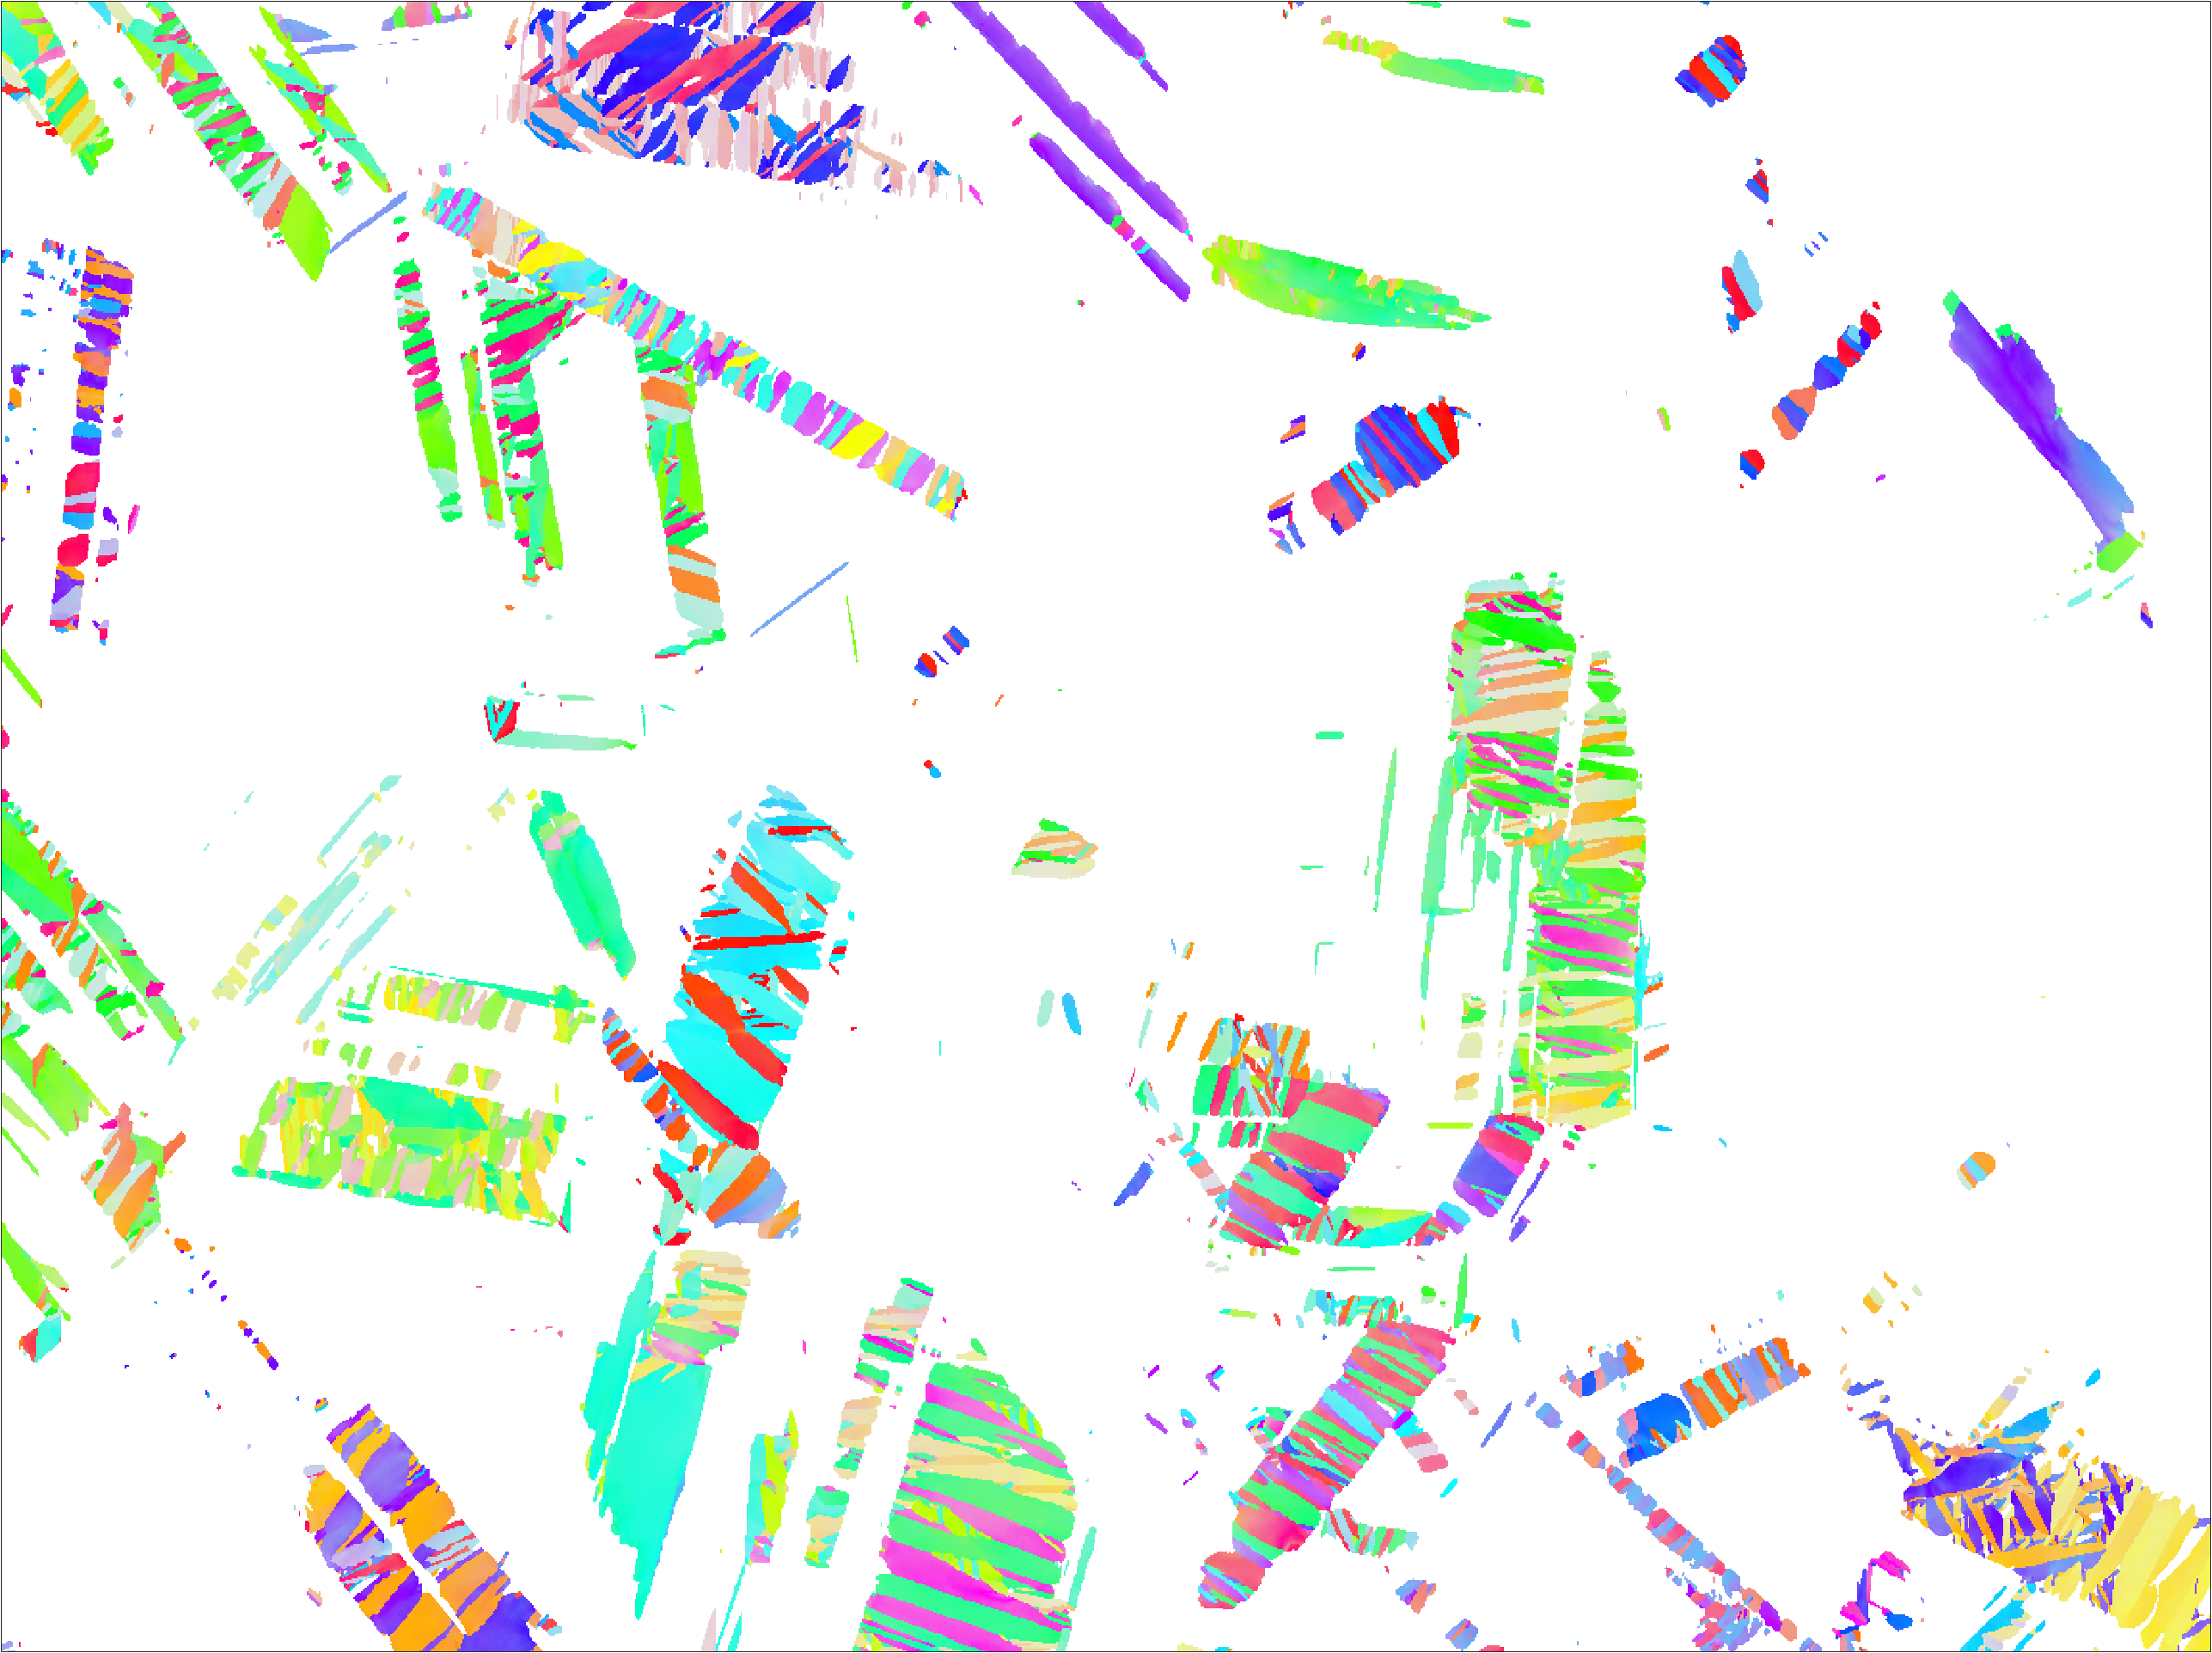
\includegraphics[width=0.3\textwidth]{pic/alphaRaw}

  \hspace{2.04cm} $\gamma$ \hspace{2.04cm} $\to$
  \hspace{2.04cm} $\varepsilon$ \hspace{2.04cm} $\to$
  \hspace{2.04cm} $\alpha'$

  \bigskip

  \begin{itemize}
  \item cold-rolled high-Mn steel, EBSD map courtesy: Pramanik et al.
  \item face-centered cubic parent $\gamma$ austenite
  \item partially transformed to hexagonally close-packed $\varepsilon$
    martensite
  \item partially transformed to body-centered tetragonal $\alpha'$ martensite
  \end{itemize}

\end{overlayarea}
\end{frame}

\begin{frame}[fragile]

  \frametitle{Step 1: Grain Reconstruction}

  \begin{overlayarea}{\textwidth}{0.85\textheight}

    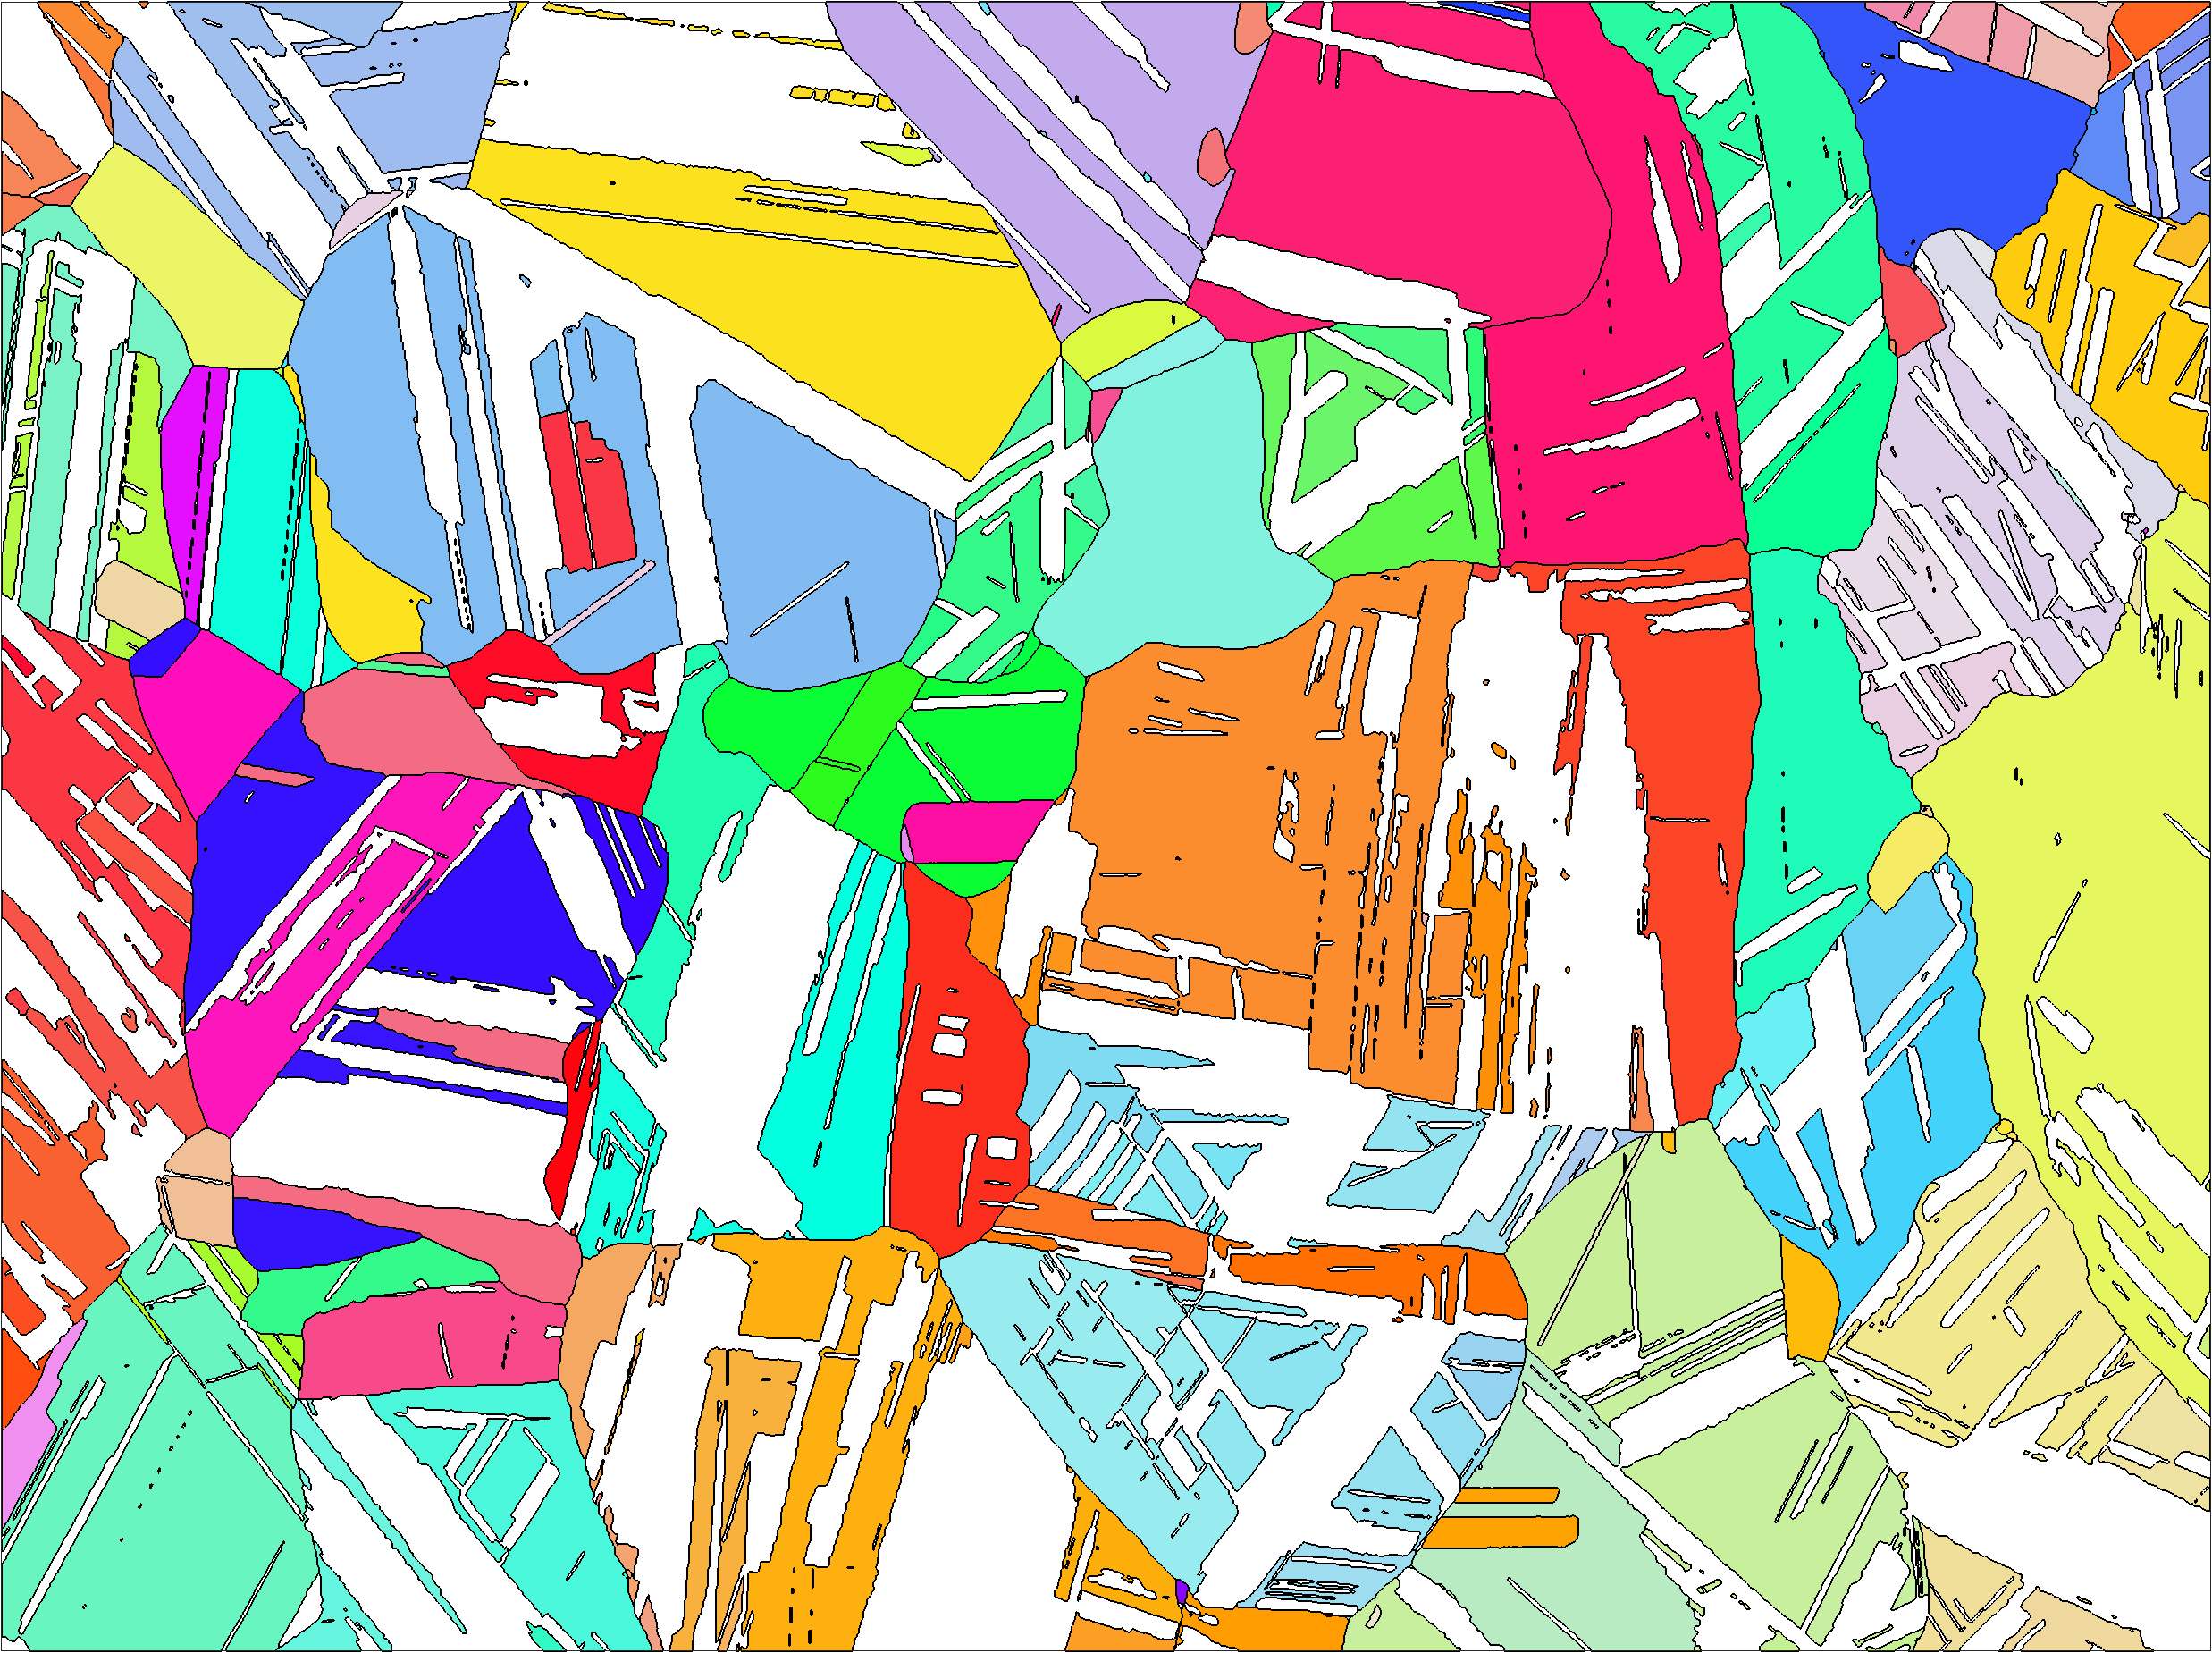
\includegraphics[width=0.3\textwidth]{pic/gammaGrains}
    \quad
    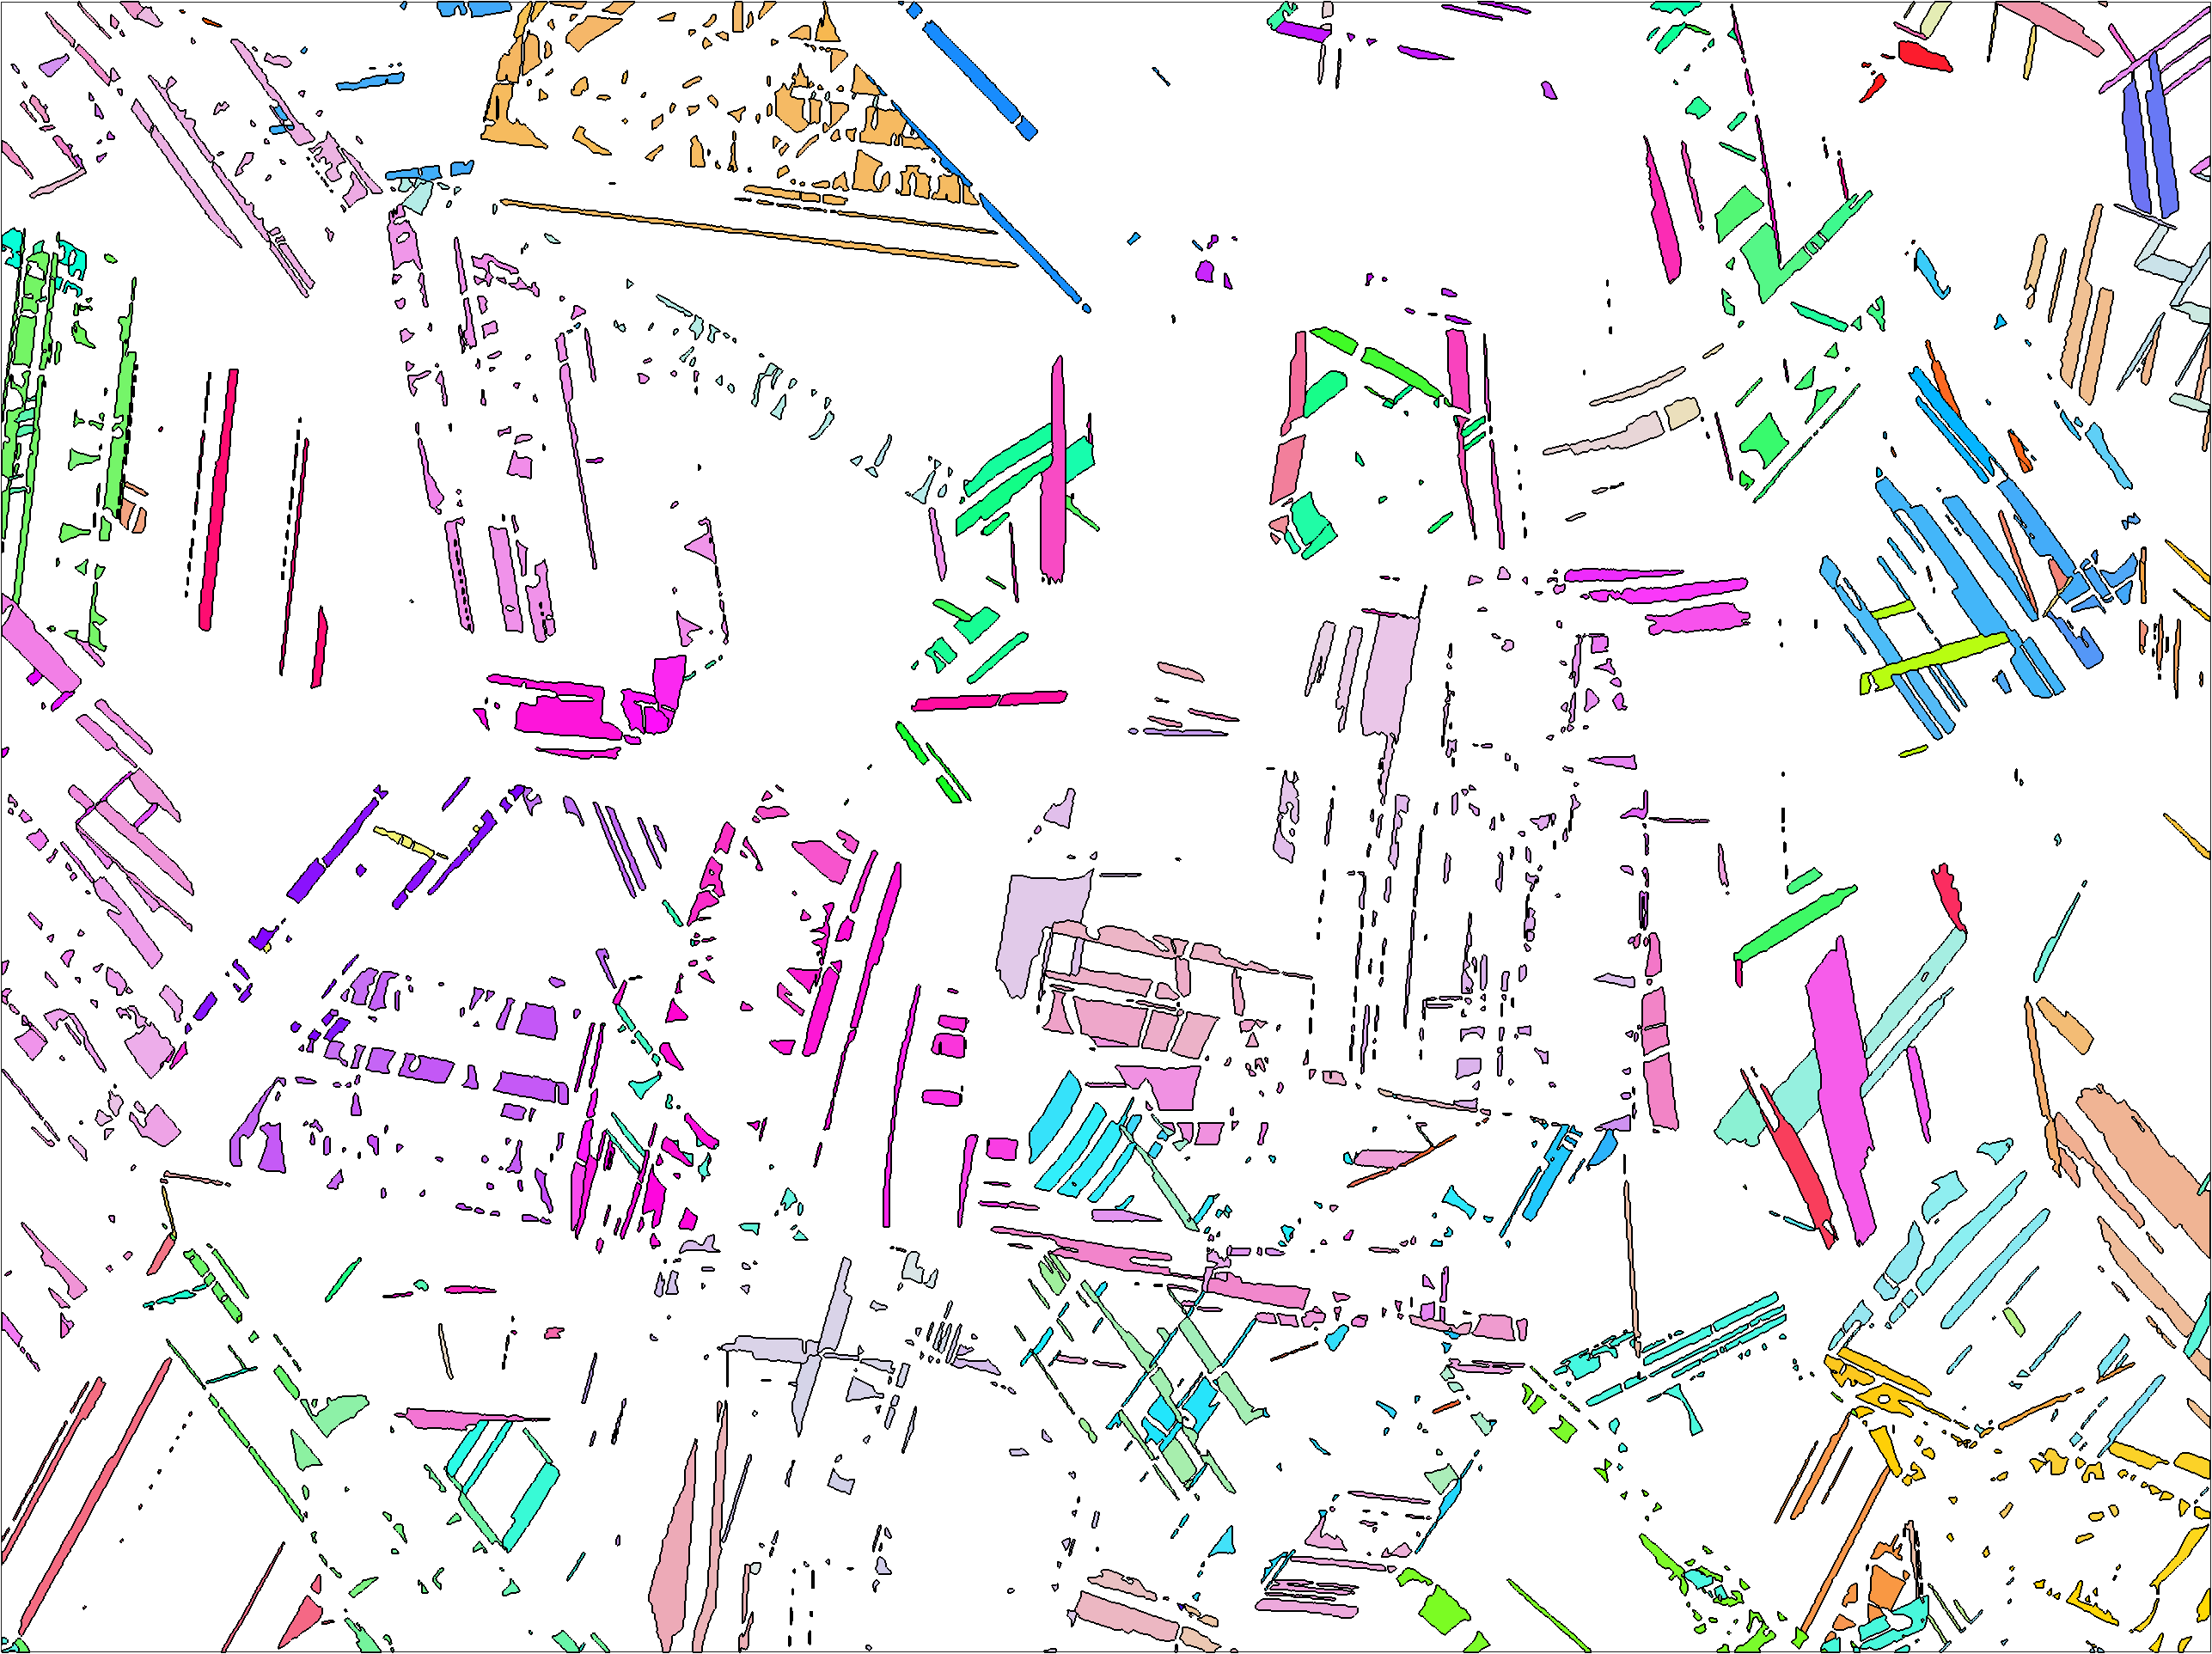
\includegraphics[width=0.3\textwidth]{pic/EpsGrains}
    \quad
    \includegraphics[width=0.3\textwidth]{pic/alphaGrains}

    \hspace{2.04cm} $\gamma$ \hspace{2.04cm} $\to$
    \hspace{2.04cm} $\varepsilon$ \hspace{2.04cm} $\to$
    \hspace{2.04cm} $\alpha'$

    \bigskip

\begin{lstlisting}[style=input]
[grains,ebsd.grainId] = calcGrains(ebsd)
\end{lstlisting}
    \vspace{-0.2cm}
\begin{lstlisting}[style=output]
grains = grain2d

 Phase  Grains   Pixels  Mineral  Symmetry  Crystal reference frame
     1     494  1023948    gamma      m-3m
     2    3333   298246   alphaP      m-3m
     3    1981   181392  epsilon     6/mmm       X||a*, Y||b, Z||c*

 boundary segments: 204064
 inner boundary segments: 7542
 triple points: 9493

 Properties: GOS, meanRotation
\end{lstlisting}

  \end{overlayarea}
\end{frame}


\begin{frame}[fragile]
  \frametitle{The \texttt{parentGrainReconstructor}}

  \begin{overlayarea}{\textwidth}{0.85\textheight}

  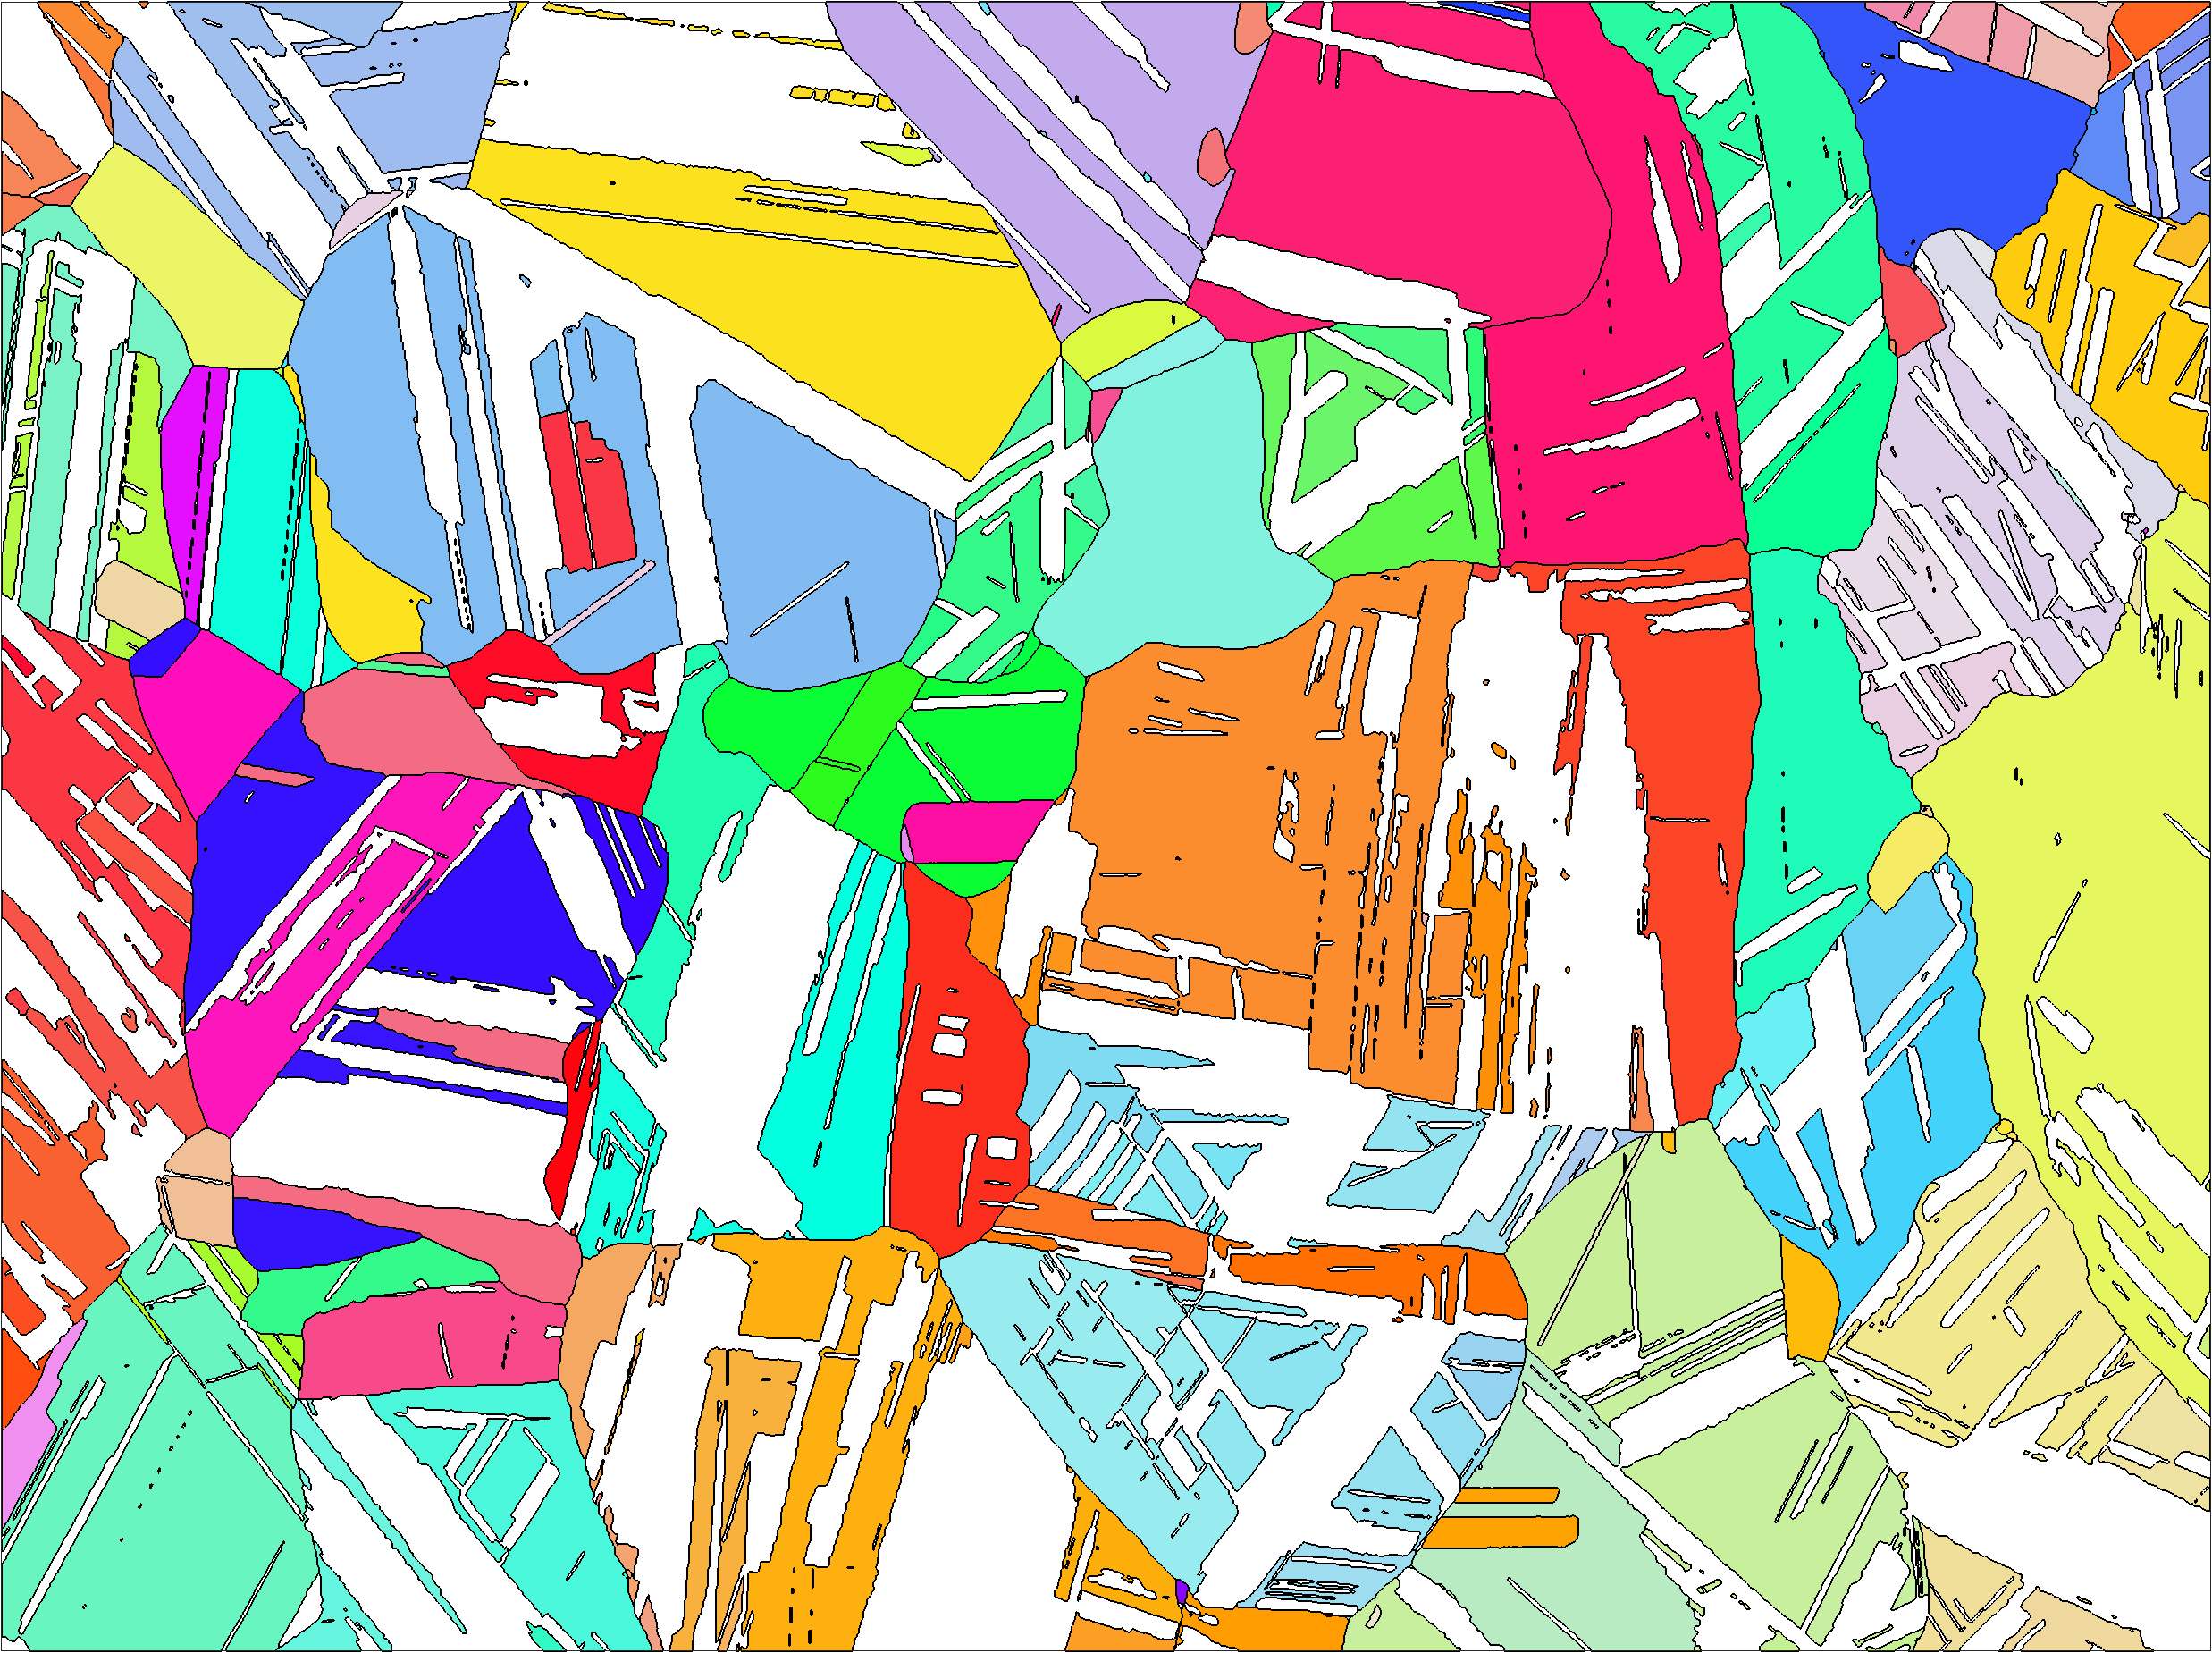
\includegraphics[width=0.3\textwidth]{pic/gammaGrains}
  \quad
  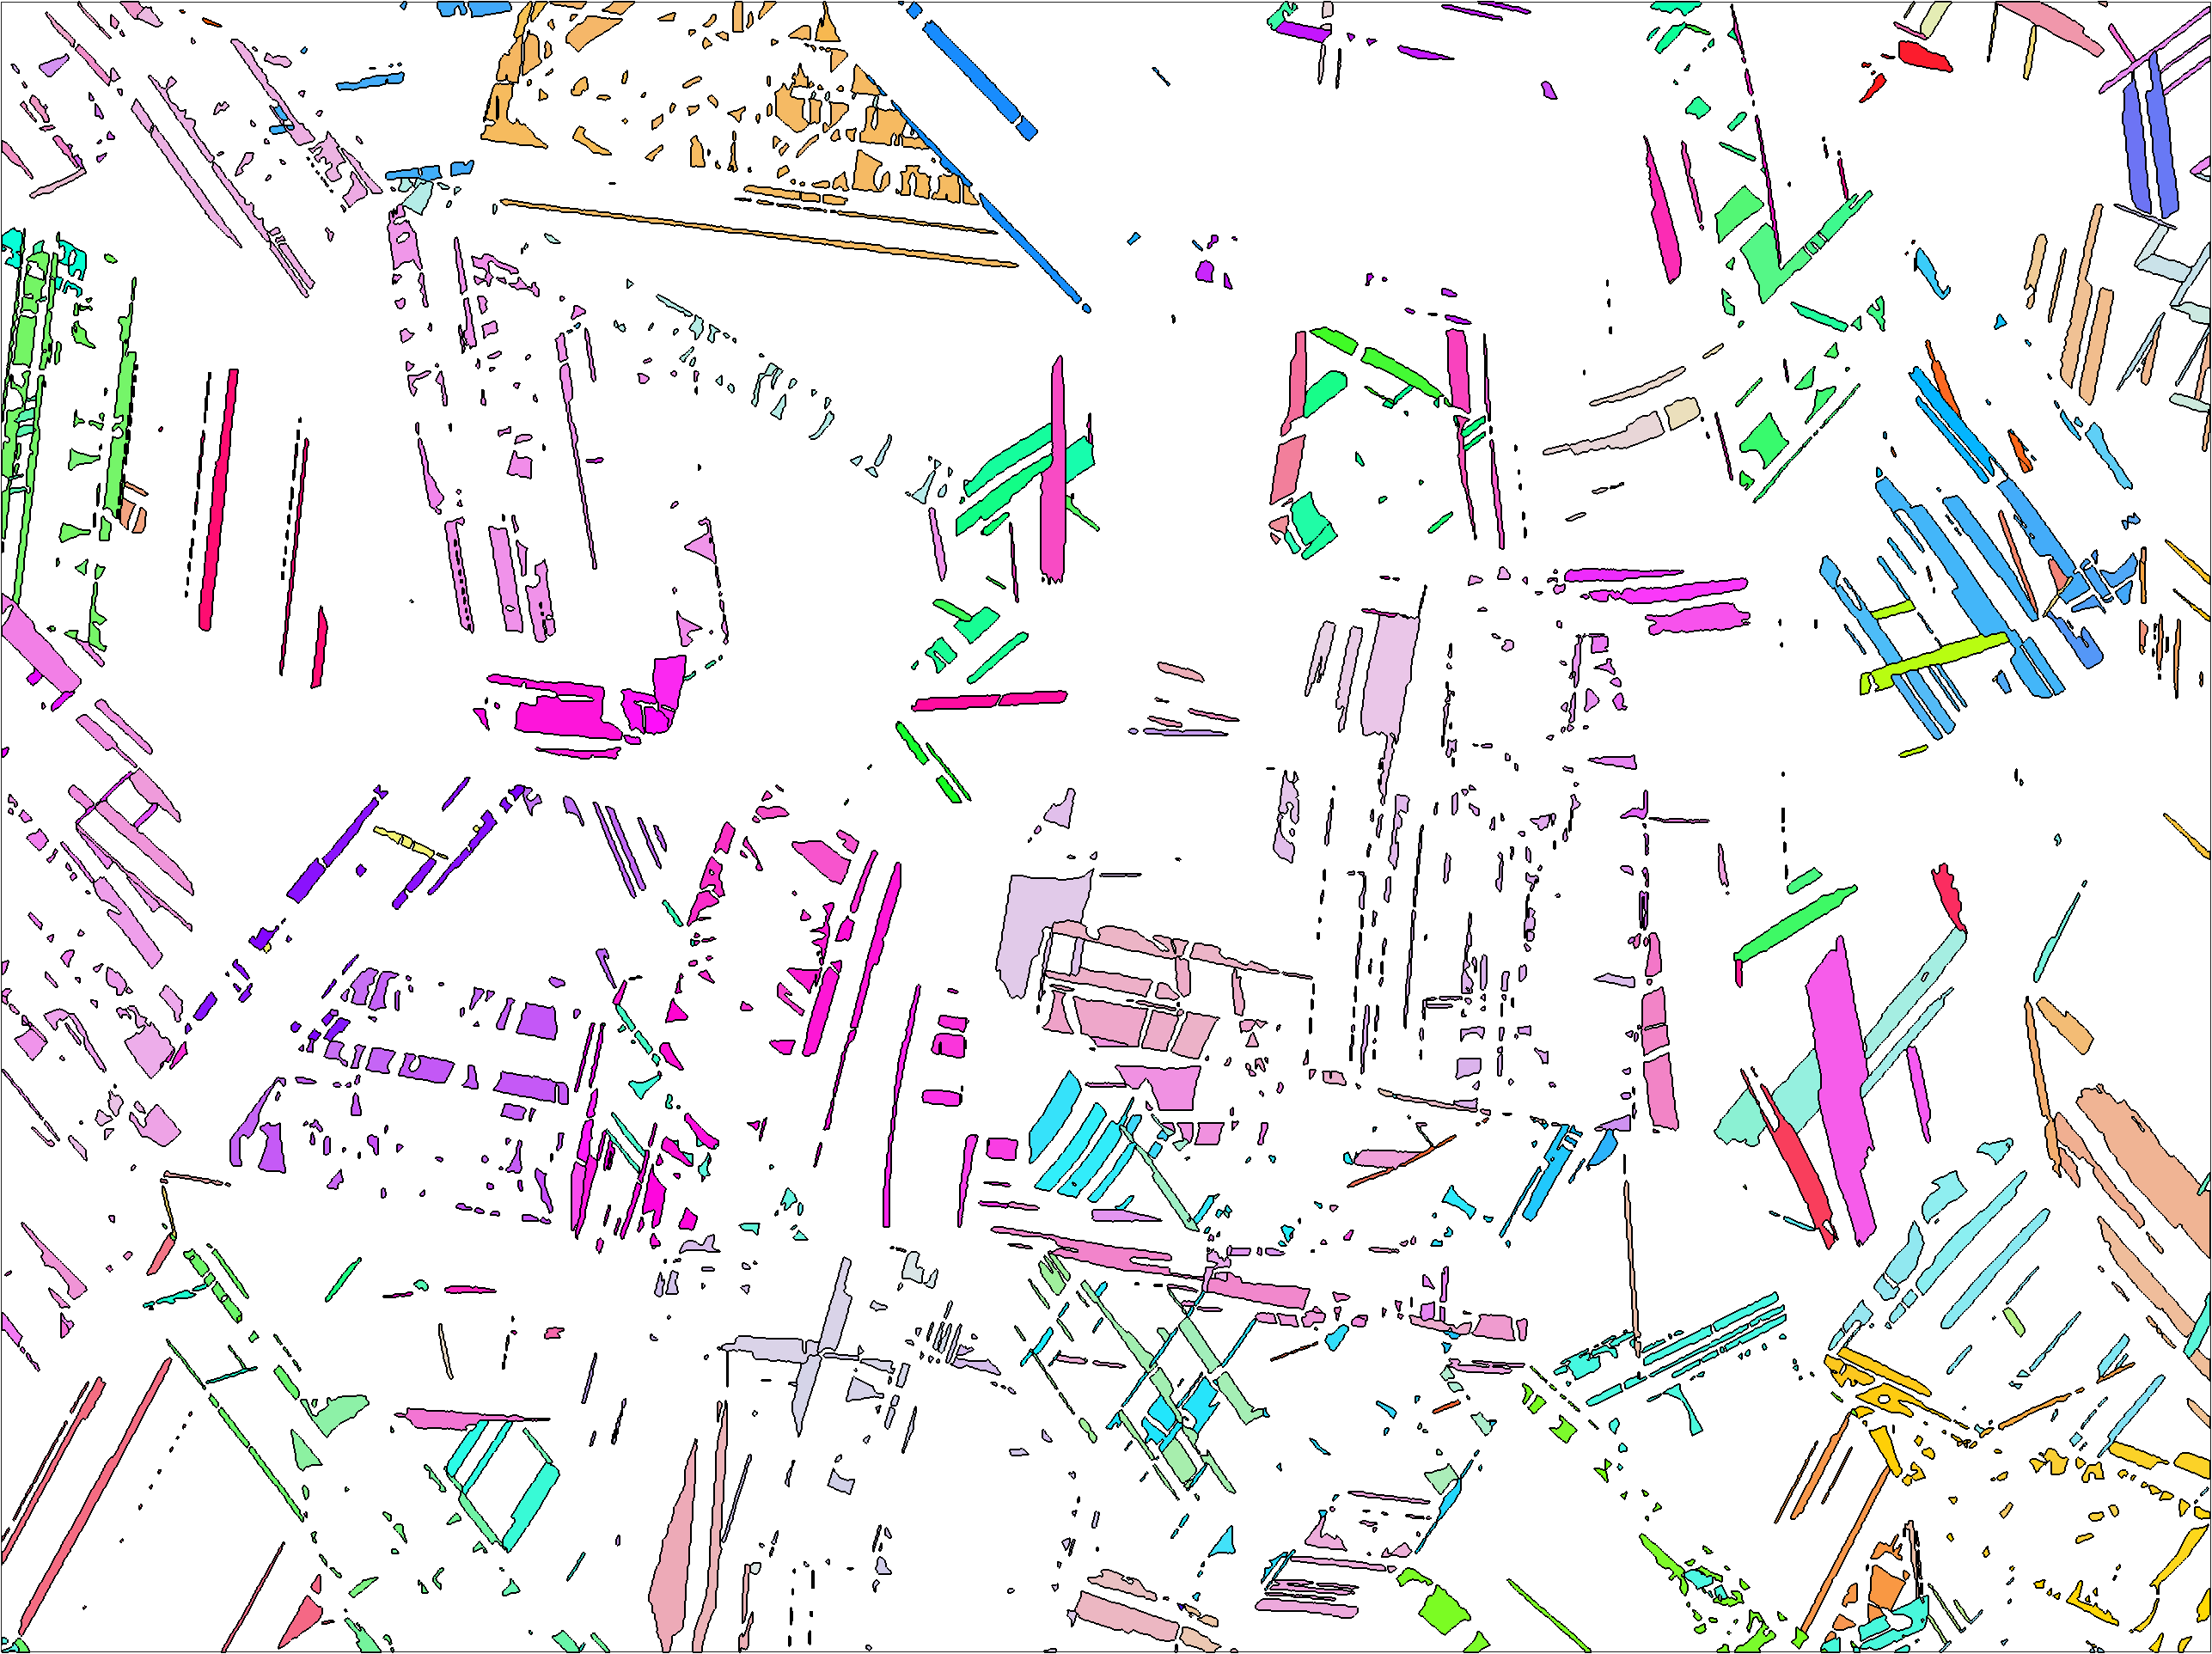
\includegraphics[width=0.3\textwidth]{pic/EpsGrains}
  \quad
  \includegraphics[width=0.3\textwidth]{pic/alphaGrains}

  \hspace{2.04cm} $\gamma$ \hspace{2.04cm} $\to$
  \hspace{2.04cm} $\varepsilon$ \hspace{2.04cm} $\to$
  \hspace{2.04cm} $\alpha'$

\bigskip

    \begin{onlyenv}<2>
\begin{lstlisting}[style=input]
job = parentGrainReconstructor(ebsd,grains)
job.p2c = orientation.Burgers(csEps,csAlpha)
\end{lstlisting}
\begin{lstlisting}[style=output]
job = parentGrainReconstructor

 phase   mineral  symmetry  grains  area  reconstructed
 parent  epsilon  6/mmm     1981    12%   0%
 child   alphaP   m-3m      3333    20%

 OR: (0001) || (110) [-12-10] || [-111]
   c2c fit: 0.6°, 0.9°, 1.3°, 2.2° (quintiles)
   p2c fit: 0.8°, 1.2°, 1.6°, 2.4° (quintiles)
\end{lstlisting}
    \end{onlyenv}
    \begin{onlyenv}<1>
\begin{lstlisting}[style=input]
job = parentGrainReconstructor(ebsd,grains)
job.p2c = orientation.ShojiNishiyama(csGamma, csEps)
\end{lstlisting}
\begin{lstlisting}[style=output]
job = parentGrainReconstructor

 phase   mineral  symmetry  grains  area  reconstructed
 parent  gamma    m-3m      494     68%   0%
 child   epsilon  6/mmm     1981    12%

 OR: (111) || (0001)   [10-1] || [2-1-10]
   c2c fit: 0.4°, 0.9°, 1.7°, 4.2° (quintiles)
   p2c fit: 0.5°, 0.9°, 1.3°, 2.8° (quintiles)
\end{lstlisting}
    \end{onlyenv}

    \begin{onlyenv}<3>
\begin{lstlisting}[style=input]
job = parentGrainReconstructor(ebsd,grains)
job.p2c = orientation.KurdjumovSachs(csGamma, csAlpha)
\end{lstlisting}
\begin{lstlisting}[style=output]
job = parentGrainReconstructor

 phase   mineral  symmetry  grains  area  reconstructed
 parent  gamma    m-3m      494     68%   0%
 child   alphaP   m-3m      3333    20%

 OR: (111) || (110)   [-101] || [1-11]
   c2c fit: 0.8°, 1.3°, 1.9°, 3.2° (quintiles)
   p2c fit: 0.8°, 1.1°, 1.6°, 2.3° (quintiles)
\end{lstlisting}
    \end{onlyenv}

  \end{overlayarea}

\end{frame}
\begin{frame}[fragile]
  \frametitle{Step 2: $\varepsilon \to \alpha'$ Reconstruction}

  \begin{overlayarea}{\textwidth}{0.85\textheight}

    \begin{onlyenv}<1>
      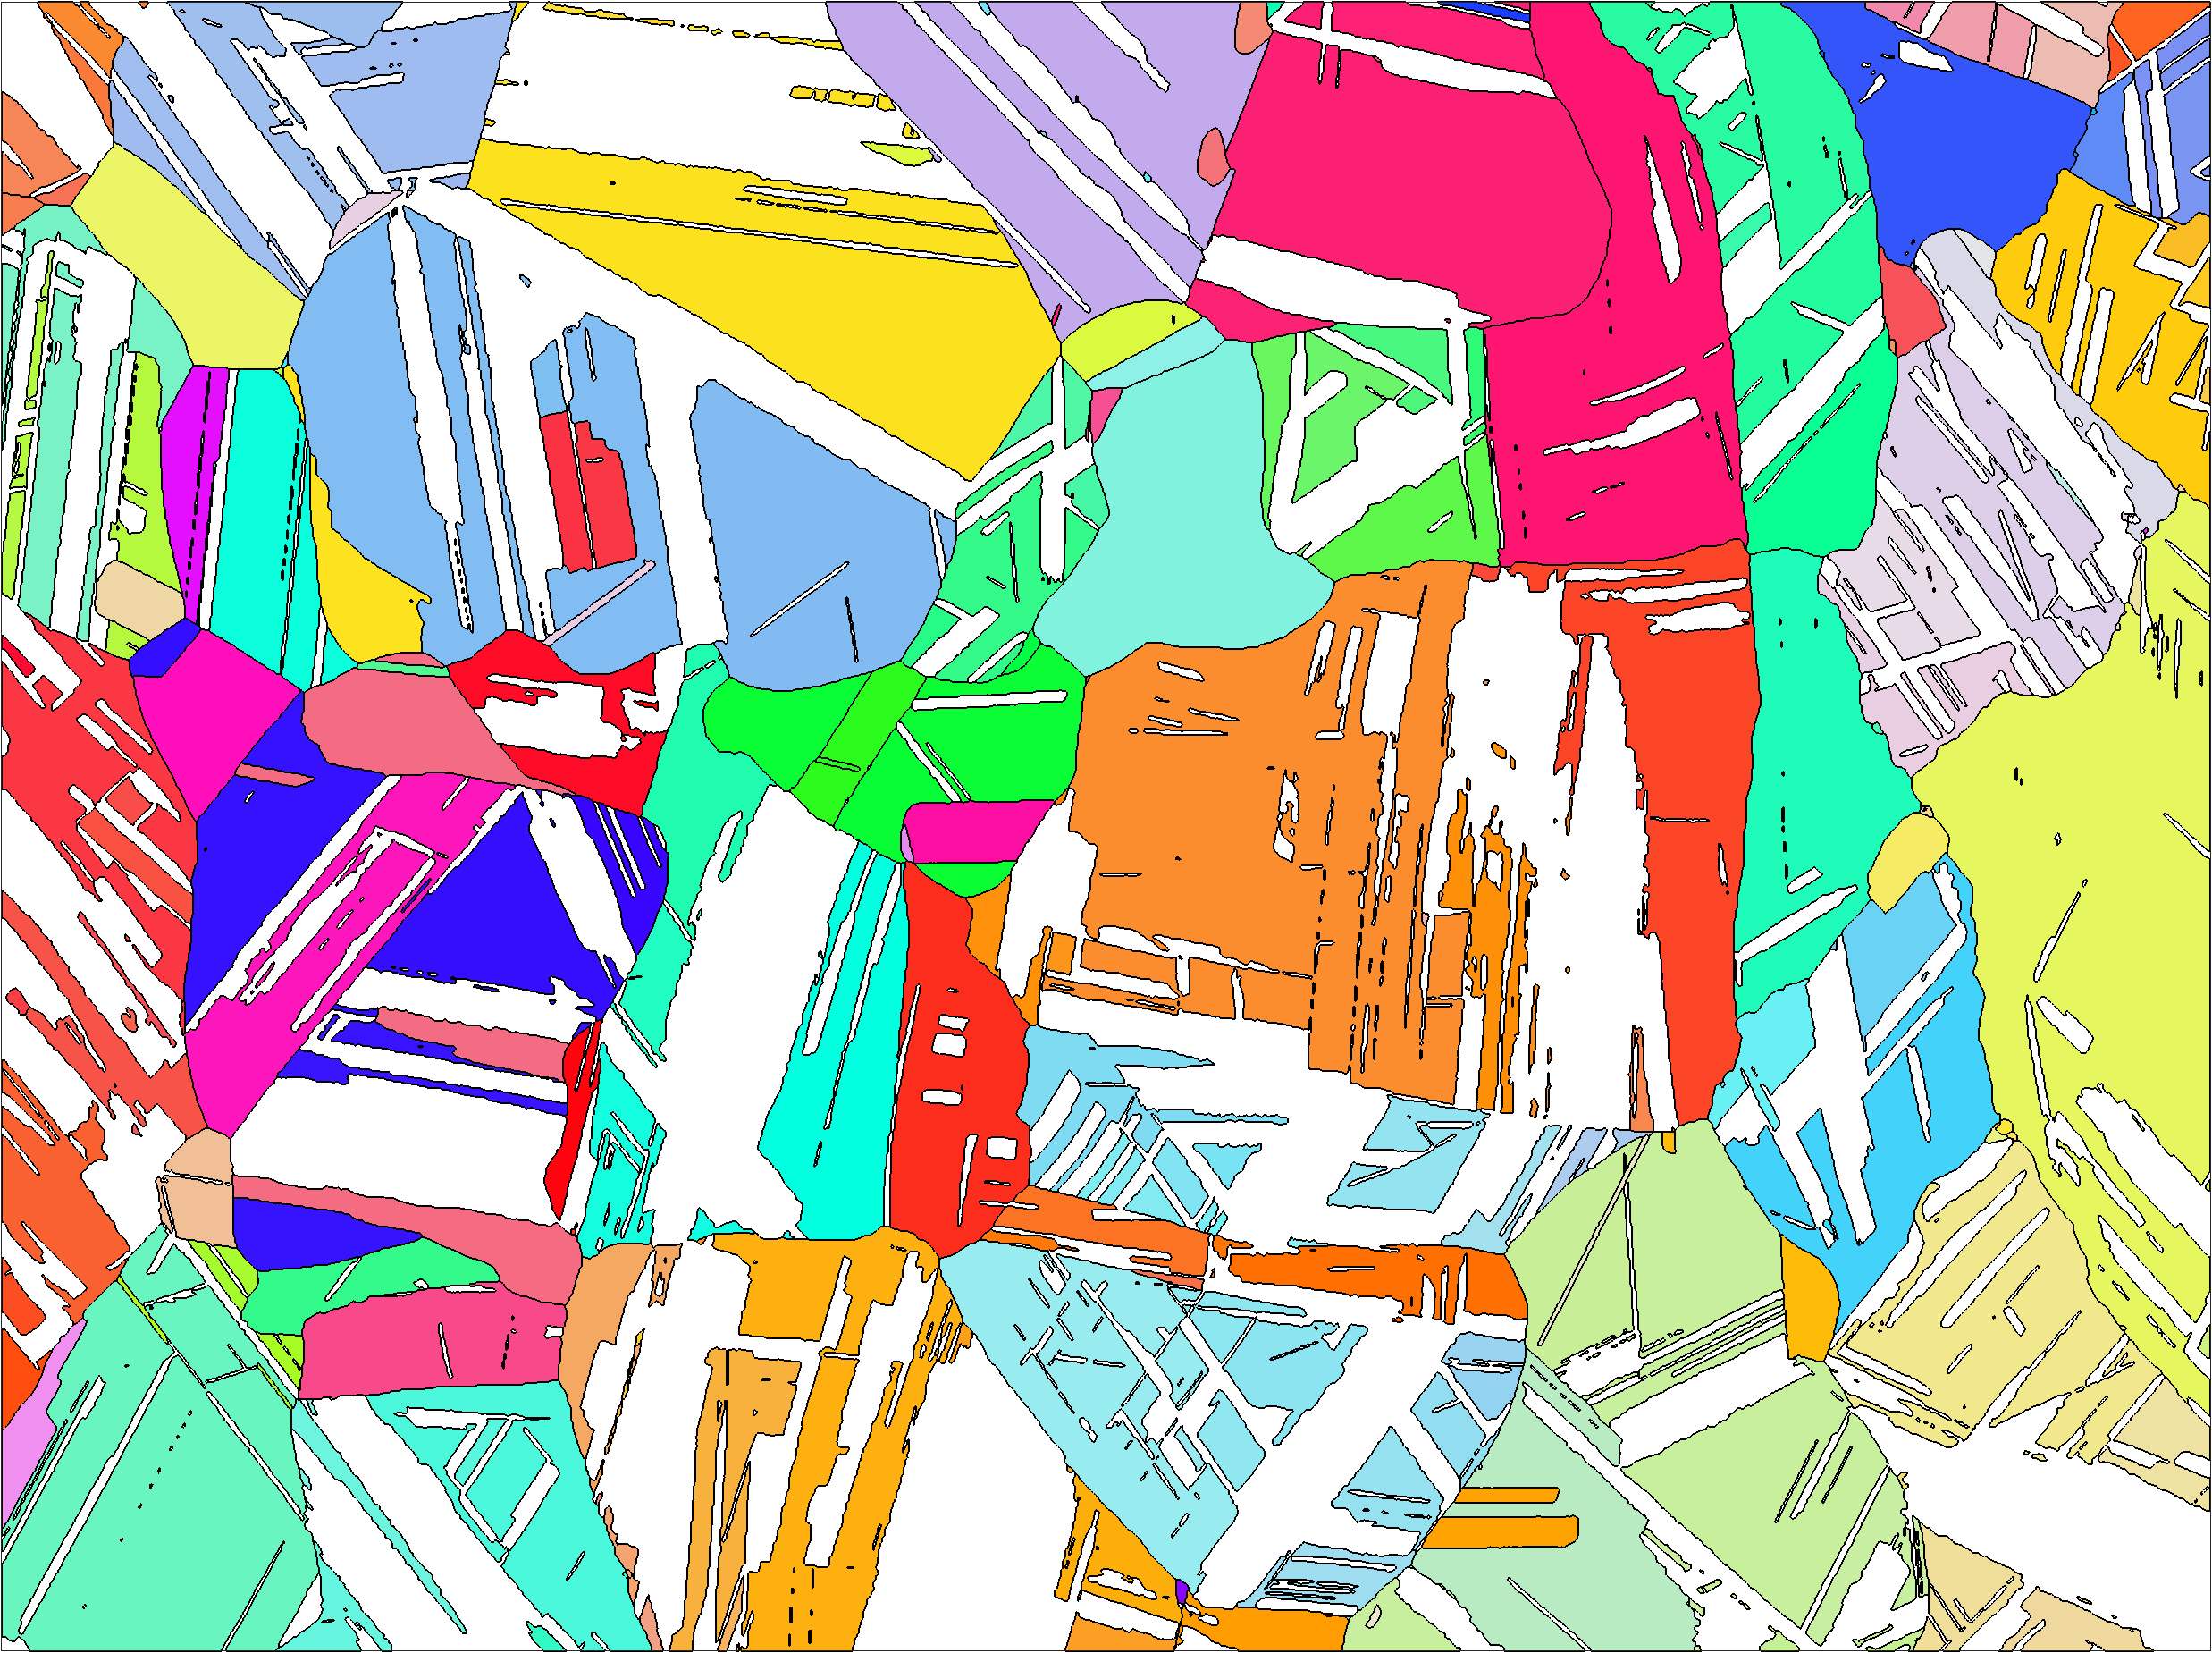
\includegraphics[width=0.3\textwidth]{pic/gammaGrains} \quad
      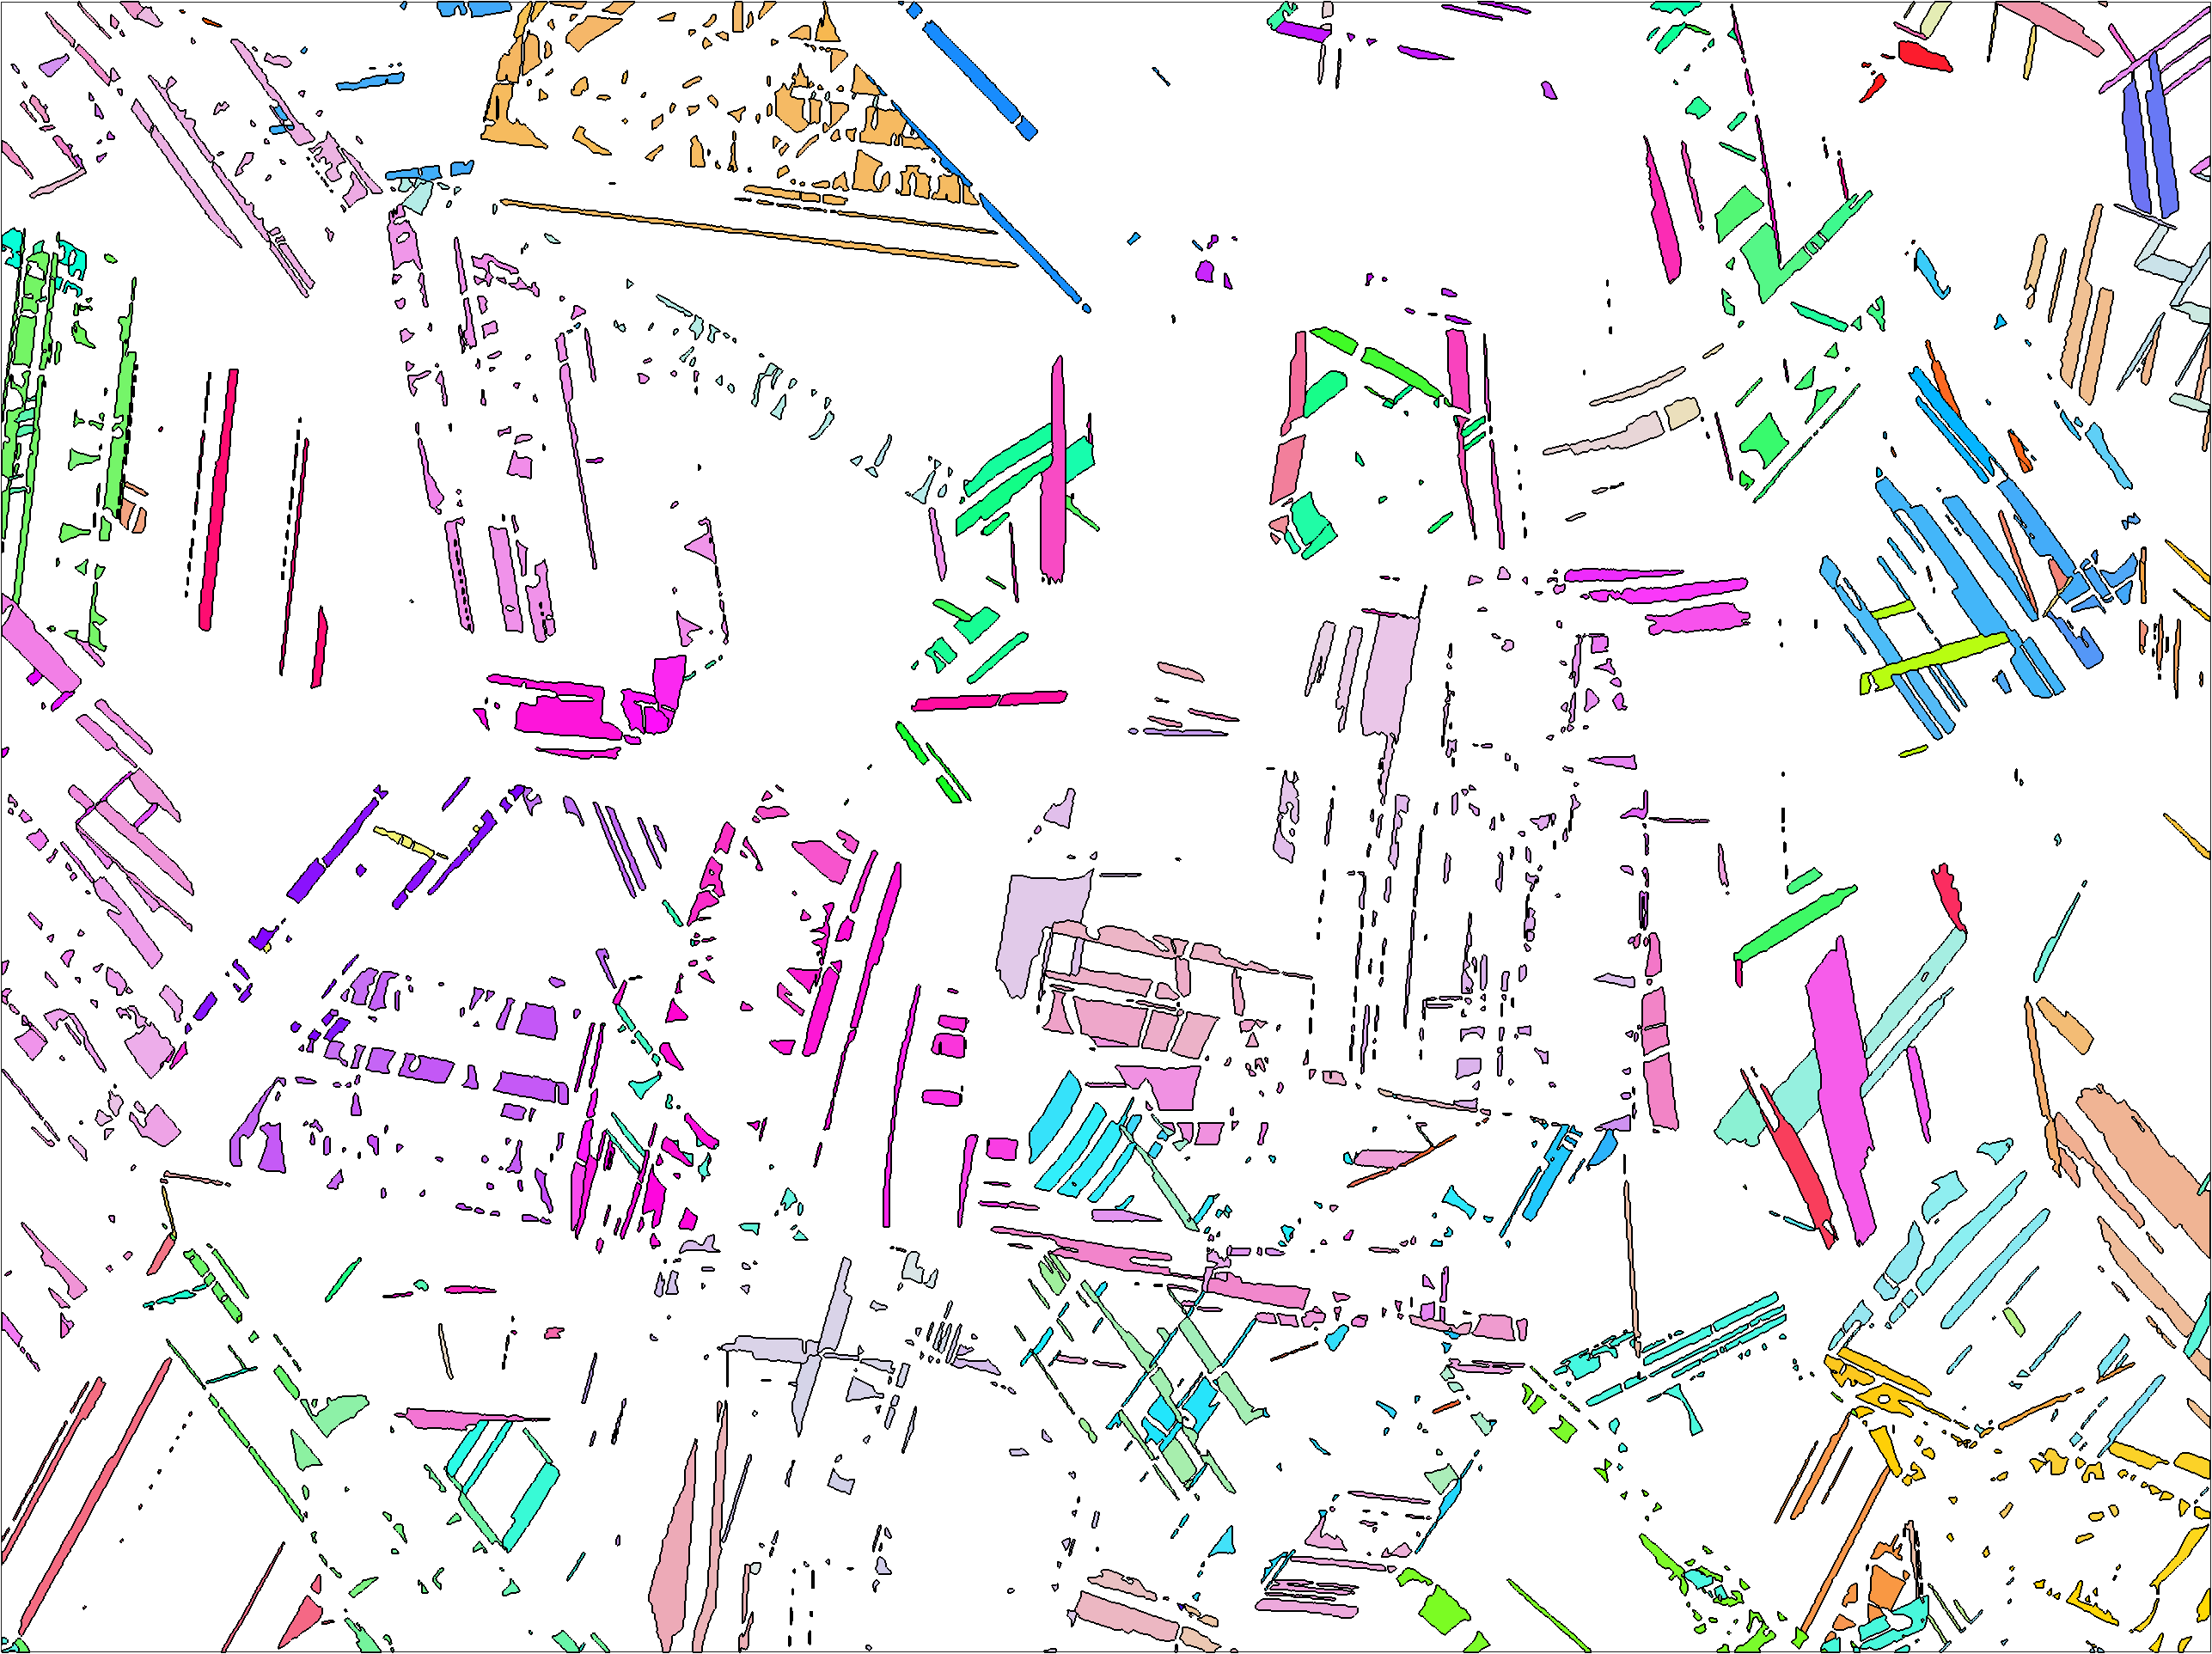
\includegraphics[width=0.3\textwidth]{pic/EpsGrains} \quad
      \includegraphics[width=0.3\textwidth]{pic/alphaGrains}
    \end{onlyenv}
    \begin{onlyenv}<2>
      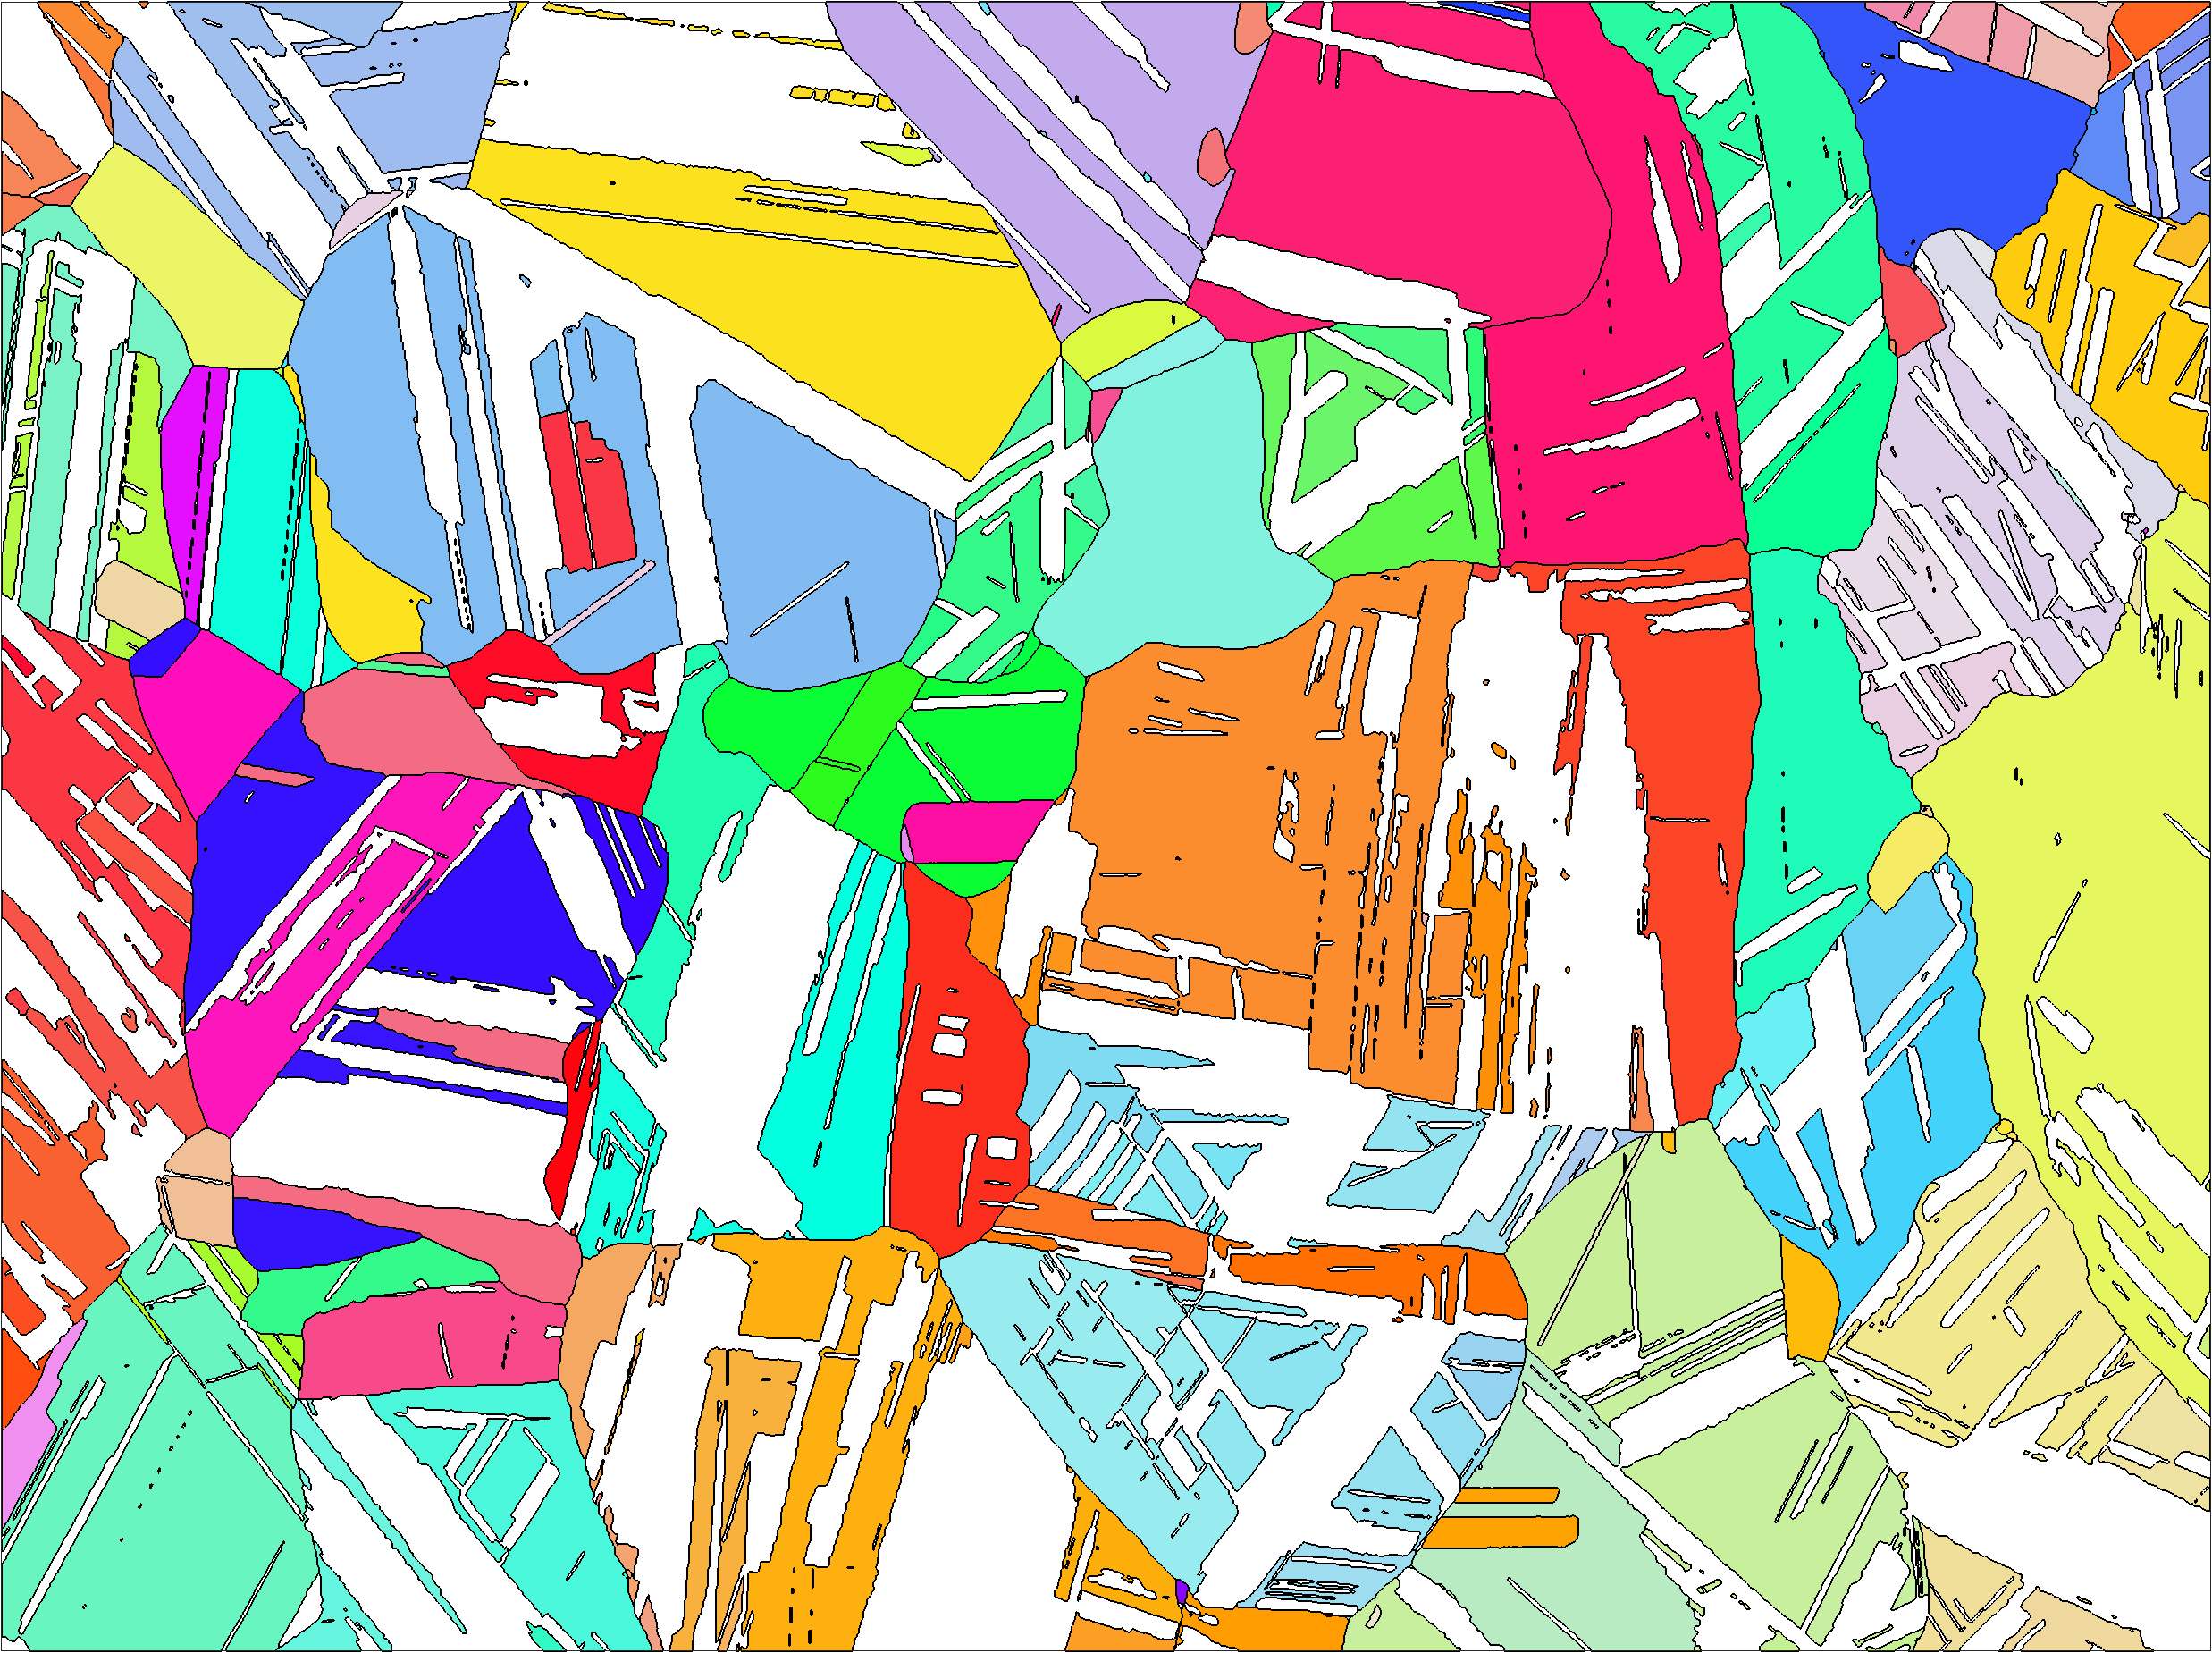
\includegraphics[width=0.3\textwidth]{pic/gammaGrains} \quad
      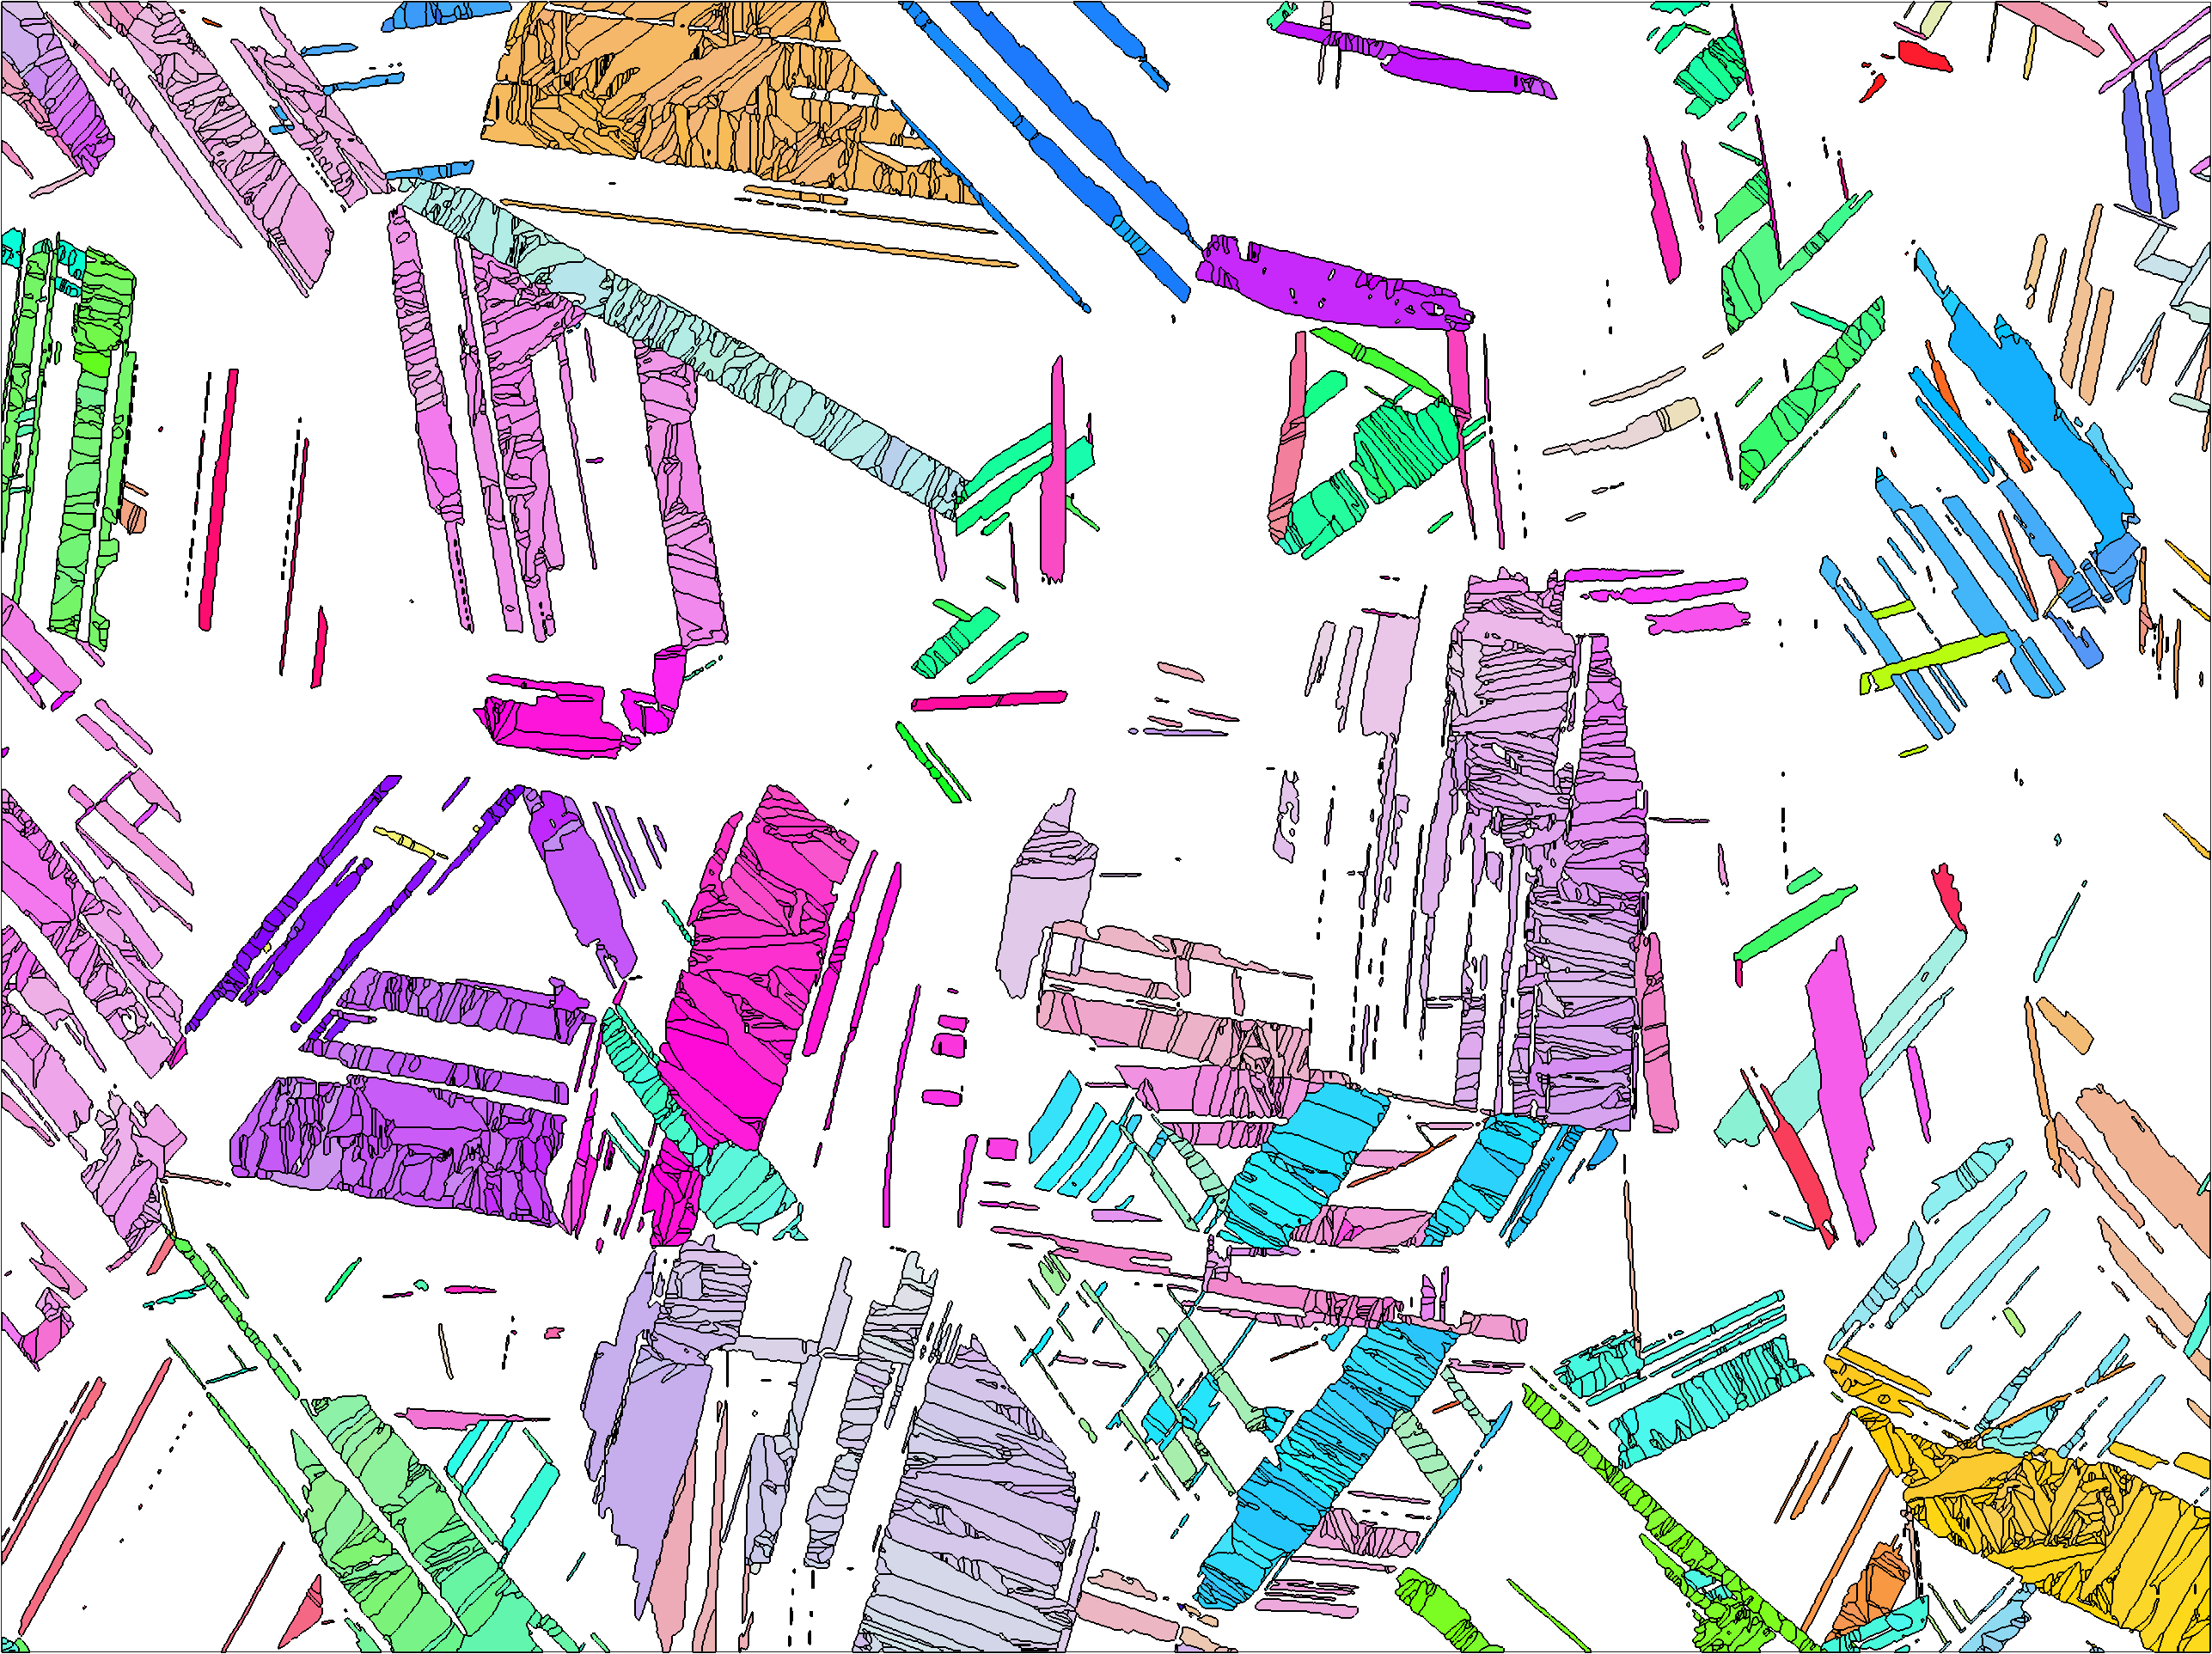
\includegraphics[width=0.3\textwidth]{pic/EpsRec_4} \quad
      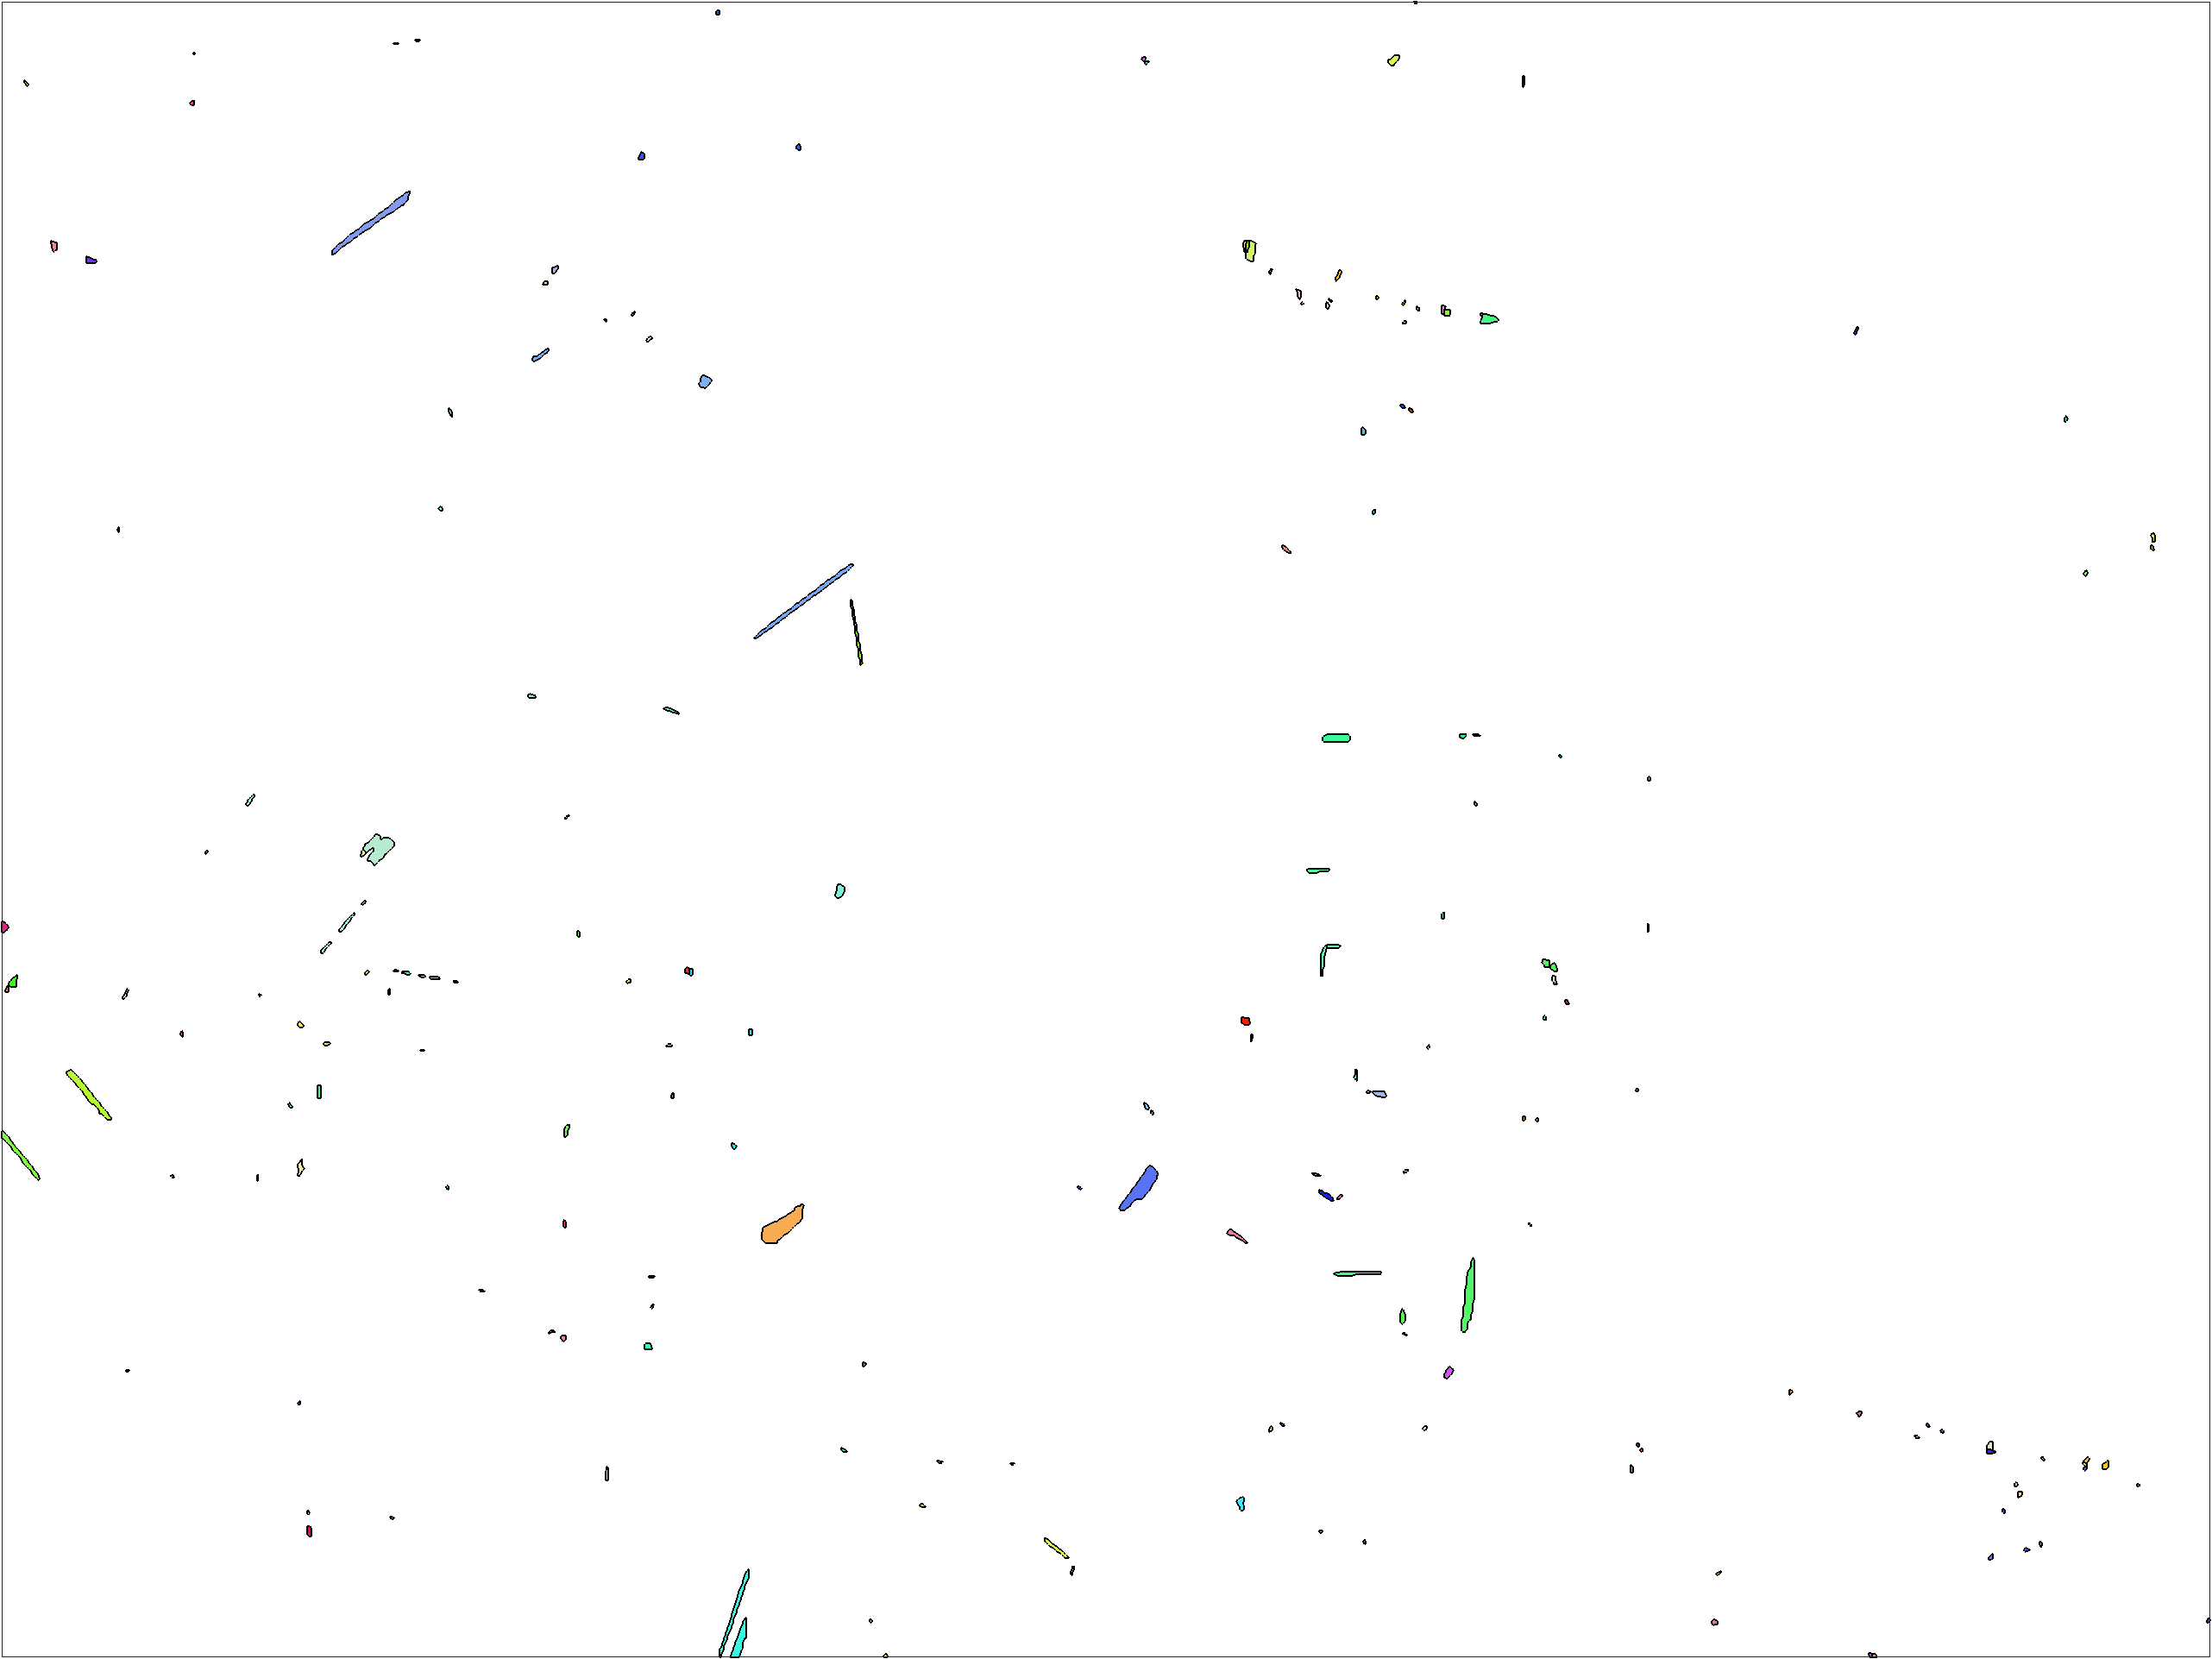
\includegraphics[width=0.3\textwidth]{pic/AlphaRec_4}
    \end{onlyenv}

    \hspace{2.04cm} $\gamma$ \hspace{2.04cm} $\to$ \hspace{2.04cm}
    $\varepsilon$ \hspace{2.04cm} $\to$ \hspace{2.04cm} $\alpha'$

    \begin{onlyenv}<1>
\begin{lstlisting}[style=input]
job.p2c = orientation.Burgers(csEps,csAlpha)
job.calcVariantGraph
job.clusterVariantGraph
\end{lstlisting}
    \end{onlyenv}
        \begin{onlyenv}<2>
\begin{lstlisting}[style=input]
job.p2c = orientation.Burgers(csEps,csAlpha)
job.calcVariantGraph
job.clusterVariantGraph
job.calcParentFromVote
\end{lstlisting}
    \end{onlyenv}
    \begin{onlyenv}<1>
      \vspace{-0.3cm}
\begin{lstlisting}[style=output]
job = parentGrainReconstructor

 phase   mineral  symmetry  grains  area  reconstructed
 parent  epsilon  6/mmm     1981    12%   0%
 child   alphaP   m-3m      3333    20%

 OR: (0001)||(110)  [-2110]||[1-11]
   c2c fit: 0.6°, 0.9°, 1.3°, 2.2° (quintiles)
   p2c fit: 0.8°, 1.2°, 1.6°, 2.4° (quintiles)

 votes: 3333 x 1
\end{lstlisting}
    \end{onlyenv}
    \begin{onlyenv}<2>
      \vspace{-0.3cm}
\begin{lstlisting}[style=output]
job = parentGrainReconstructor

 phase   mineral  symmetry  grains  area  reconstructed
 parent  epsilon  6/mmm     5117    32%   94%
 child   alphaP   m-3m      197     0.2%

 OR: (0001)||(110)  [-2110]||[1-11]
   p2c fit: 3.6°, 4.4°, 5.4°, 8.9° (quintiles)
   c2c fit: 3.3°, 3.4°, 3.8°, 8° (quintiles)
\end{lstlisting}
    \end{onlyenv}
  \end{overlayarea}

\end{frame}

\begin{frame}[fragile]
  \frametitle{Step 3: $\gamma \to \varepsilon$ Reconstruction}

  \begin{overlayarea}{\textwidth}{0.85\textheight}

    \begin{onlyenv}<1>
      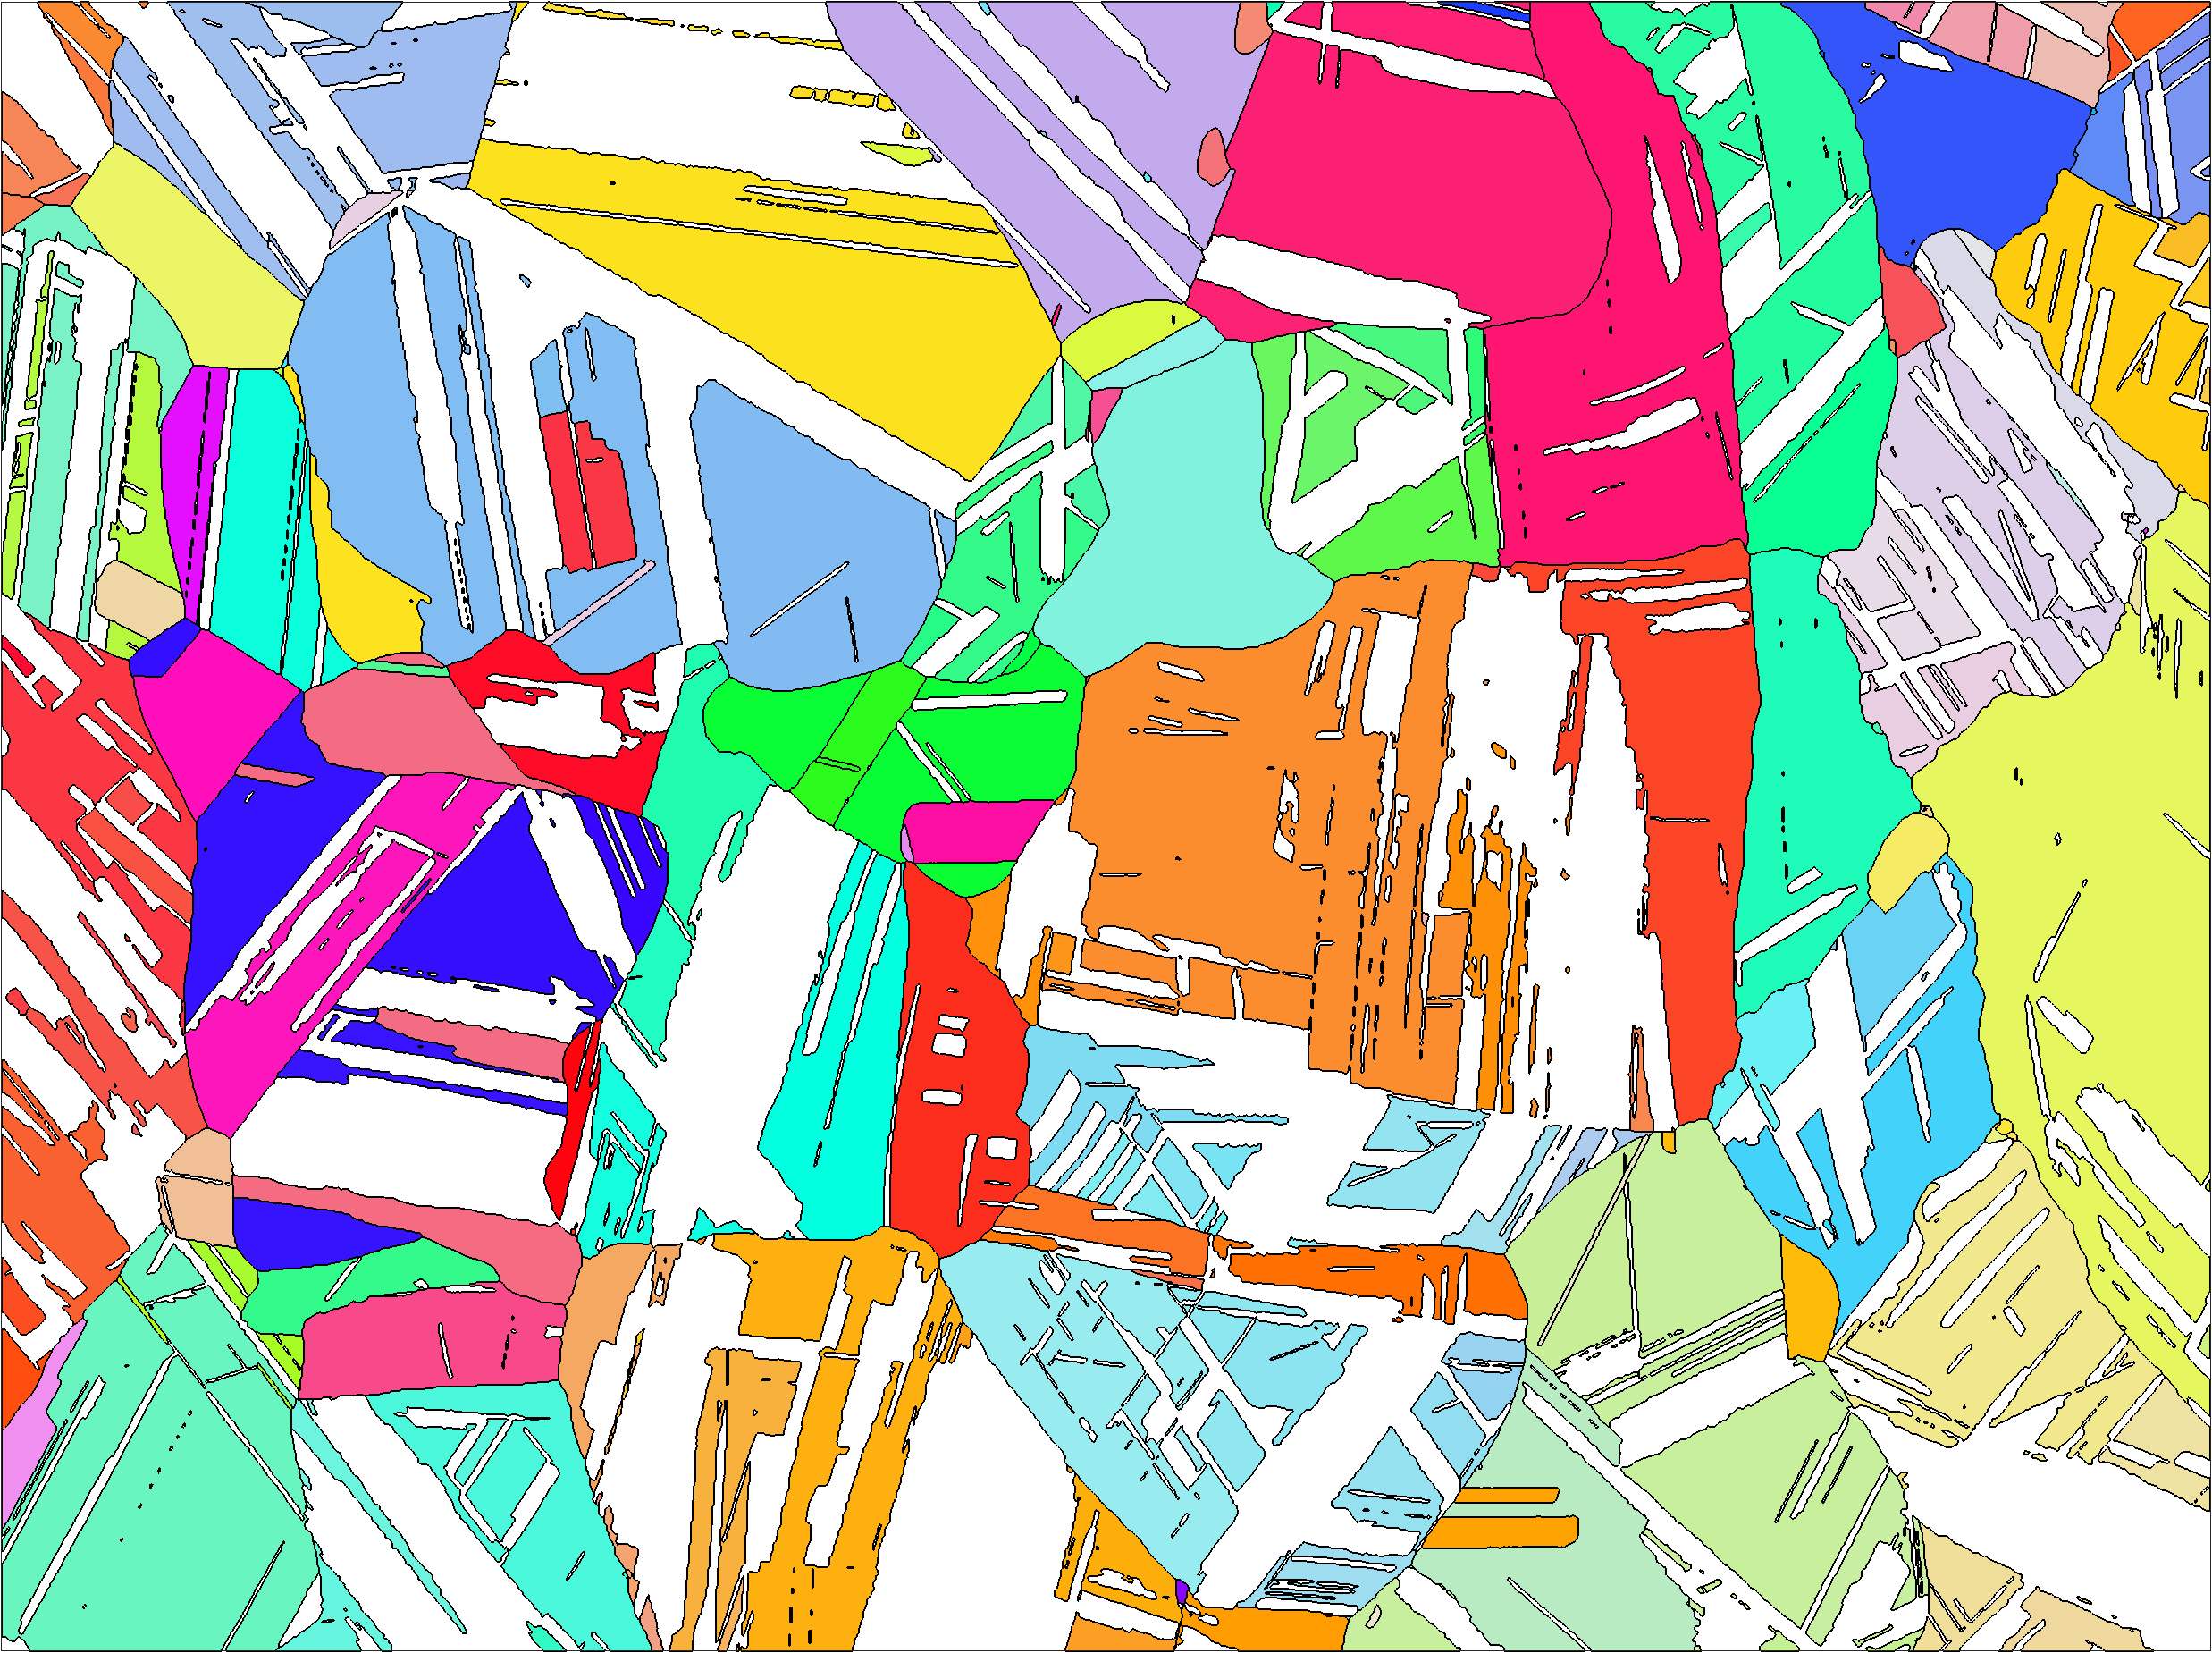
\includegraphics[width=0.3\textwidth]{pic/gammaGrains} \quad
      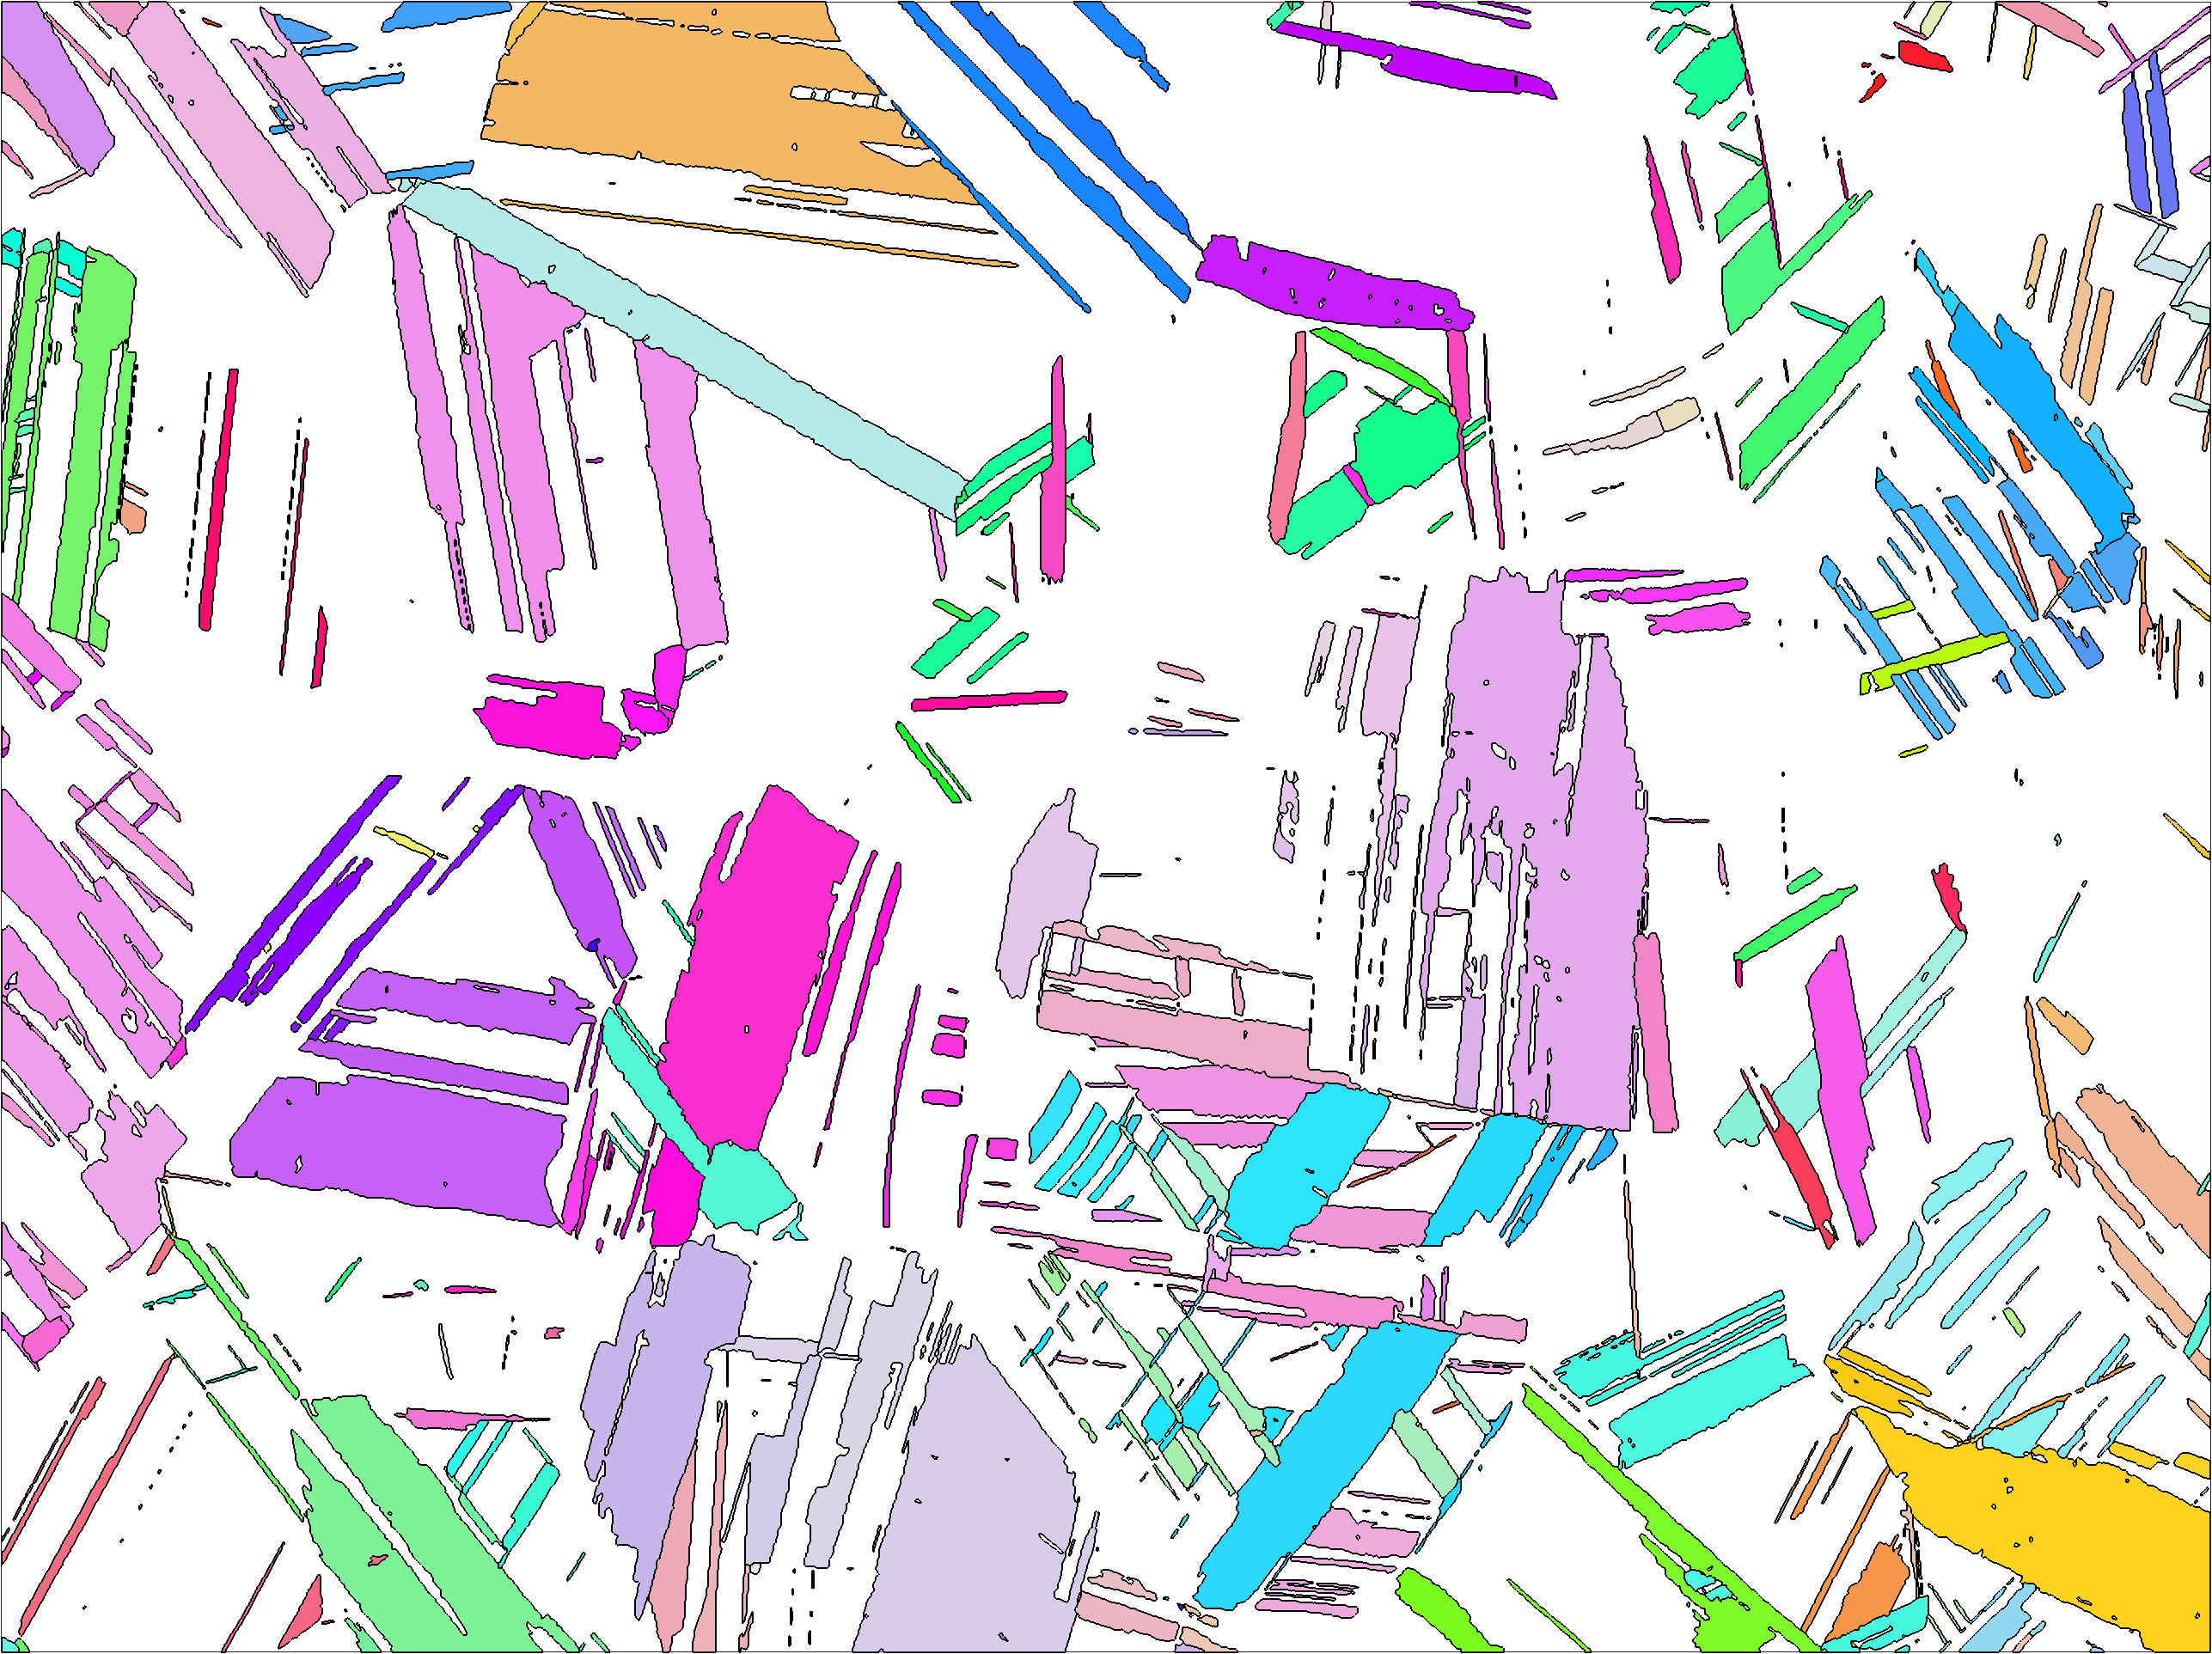
\includegraphics[width=0.3\textwidth]{pic/EpsRec_5} \quad
      \includegraphics[width=0.3\textwidth]{pic/alphaRec_4}
    \end{onlyenv}
    \begin{onlyenv}<2>
      \includegraphics[width=0.3\textwidth]{pic/gammaRec_9} \quad
      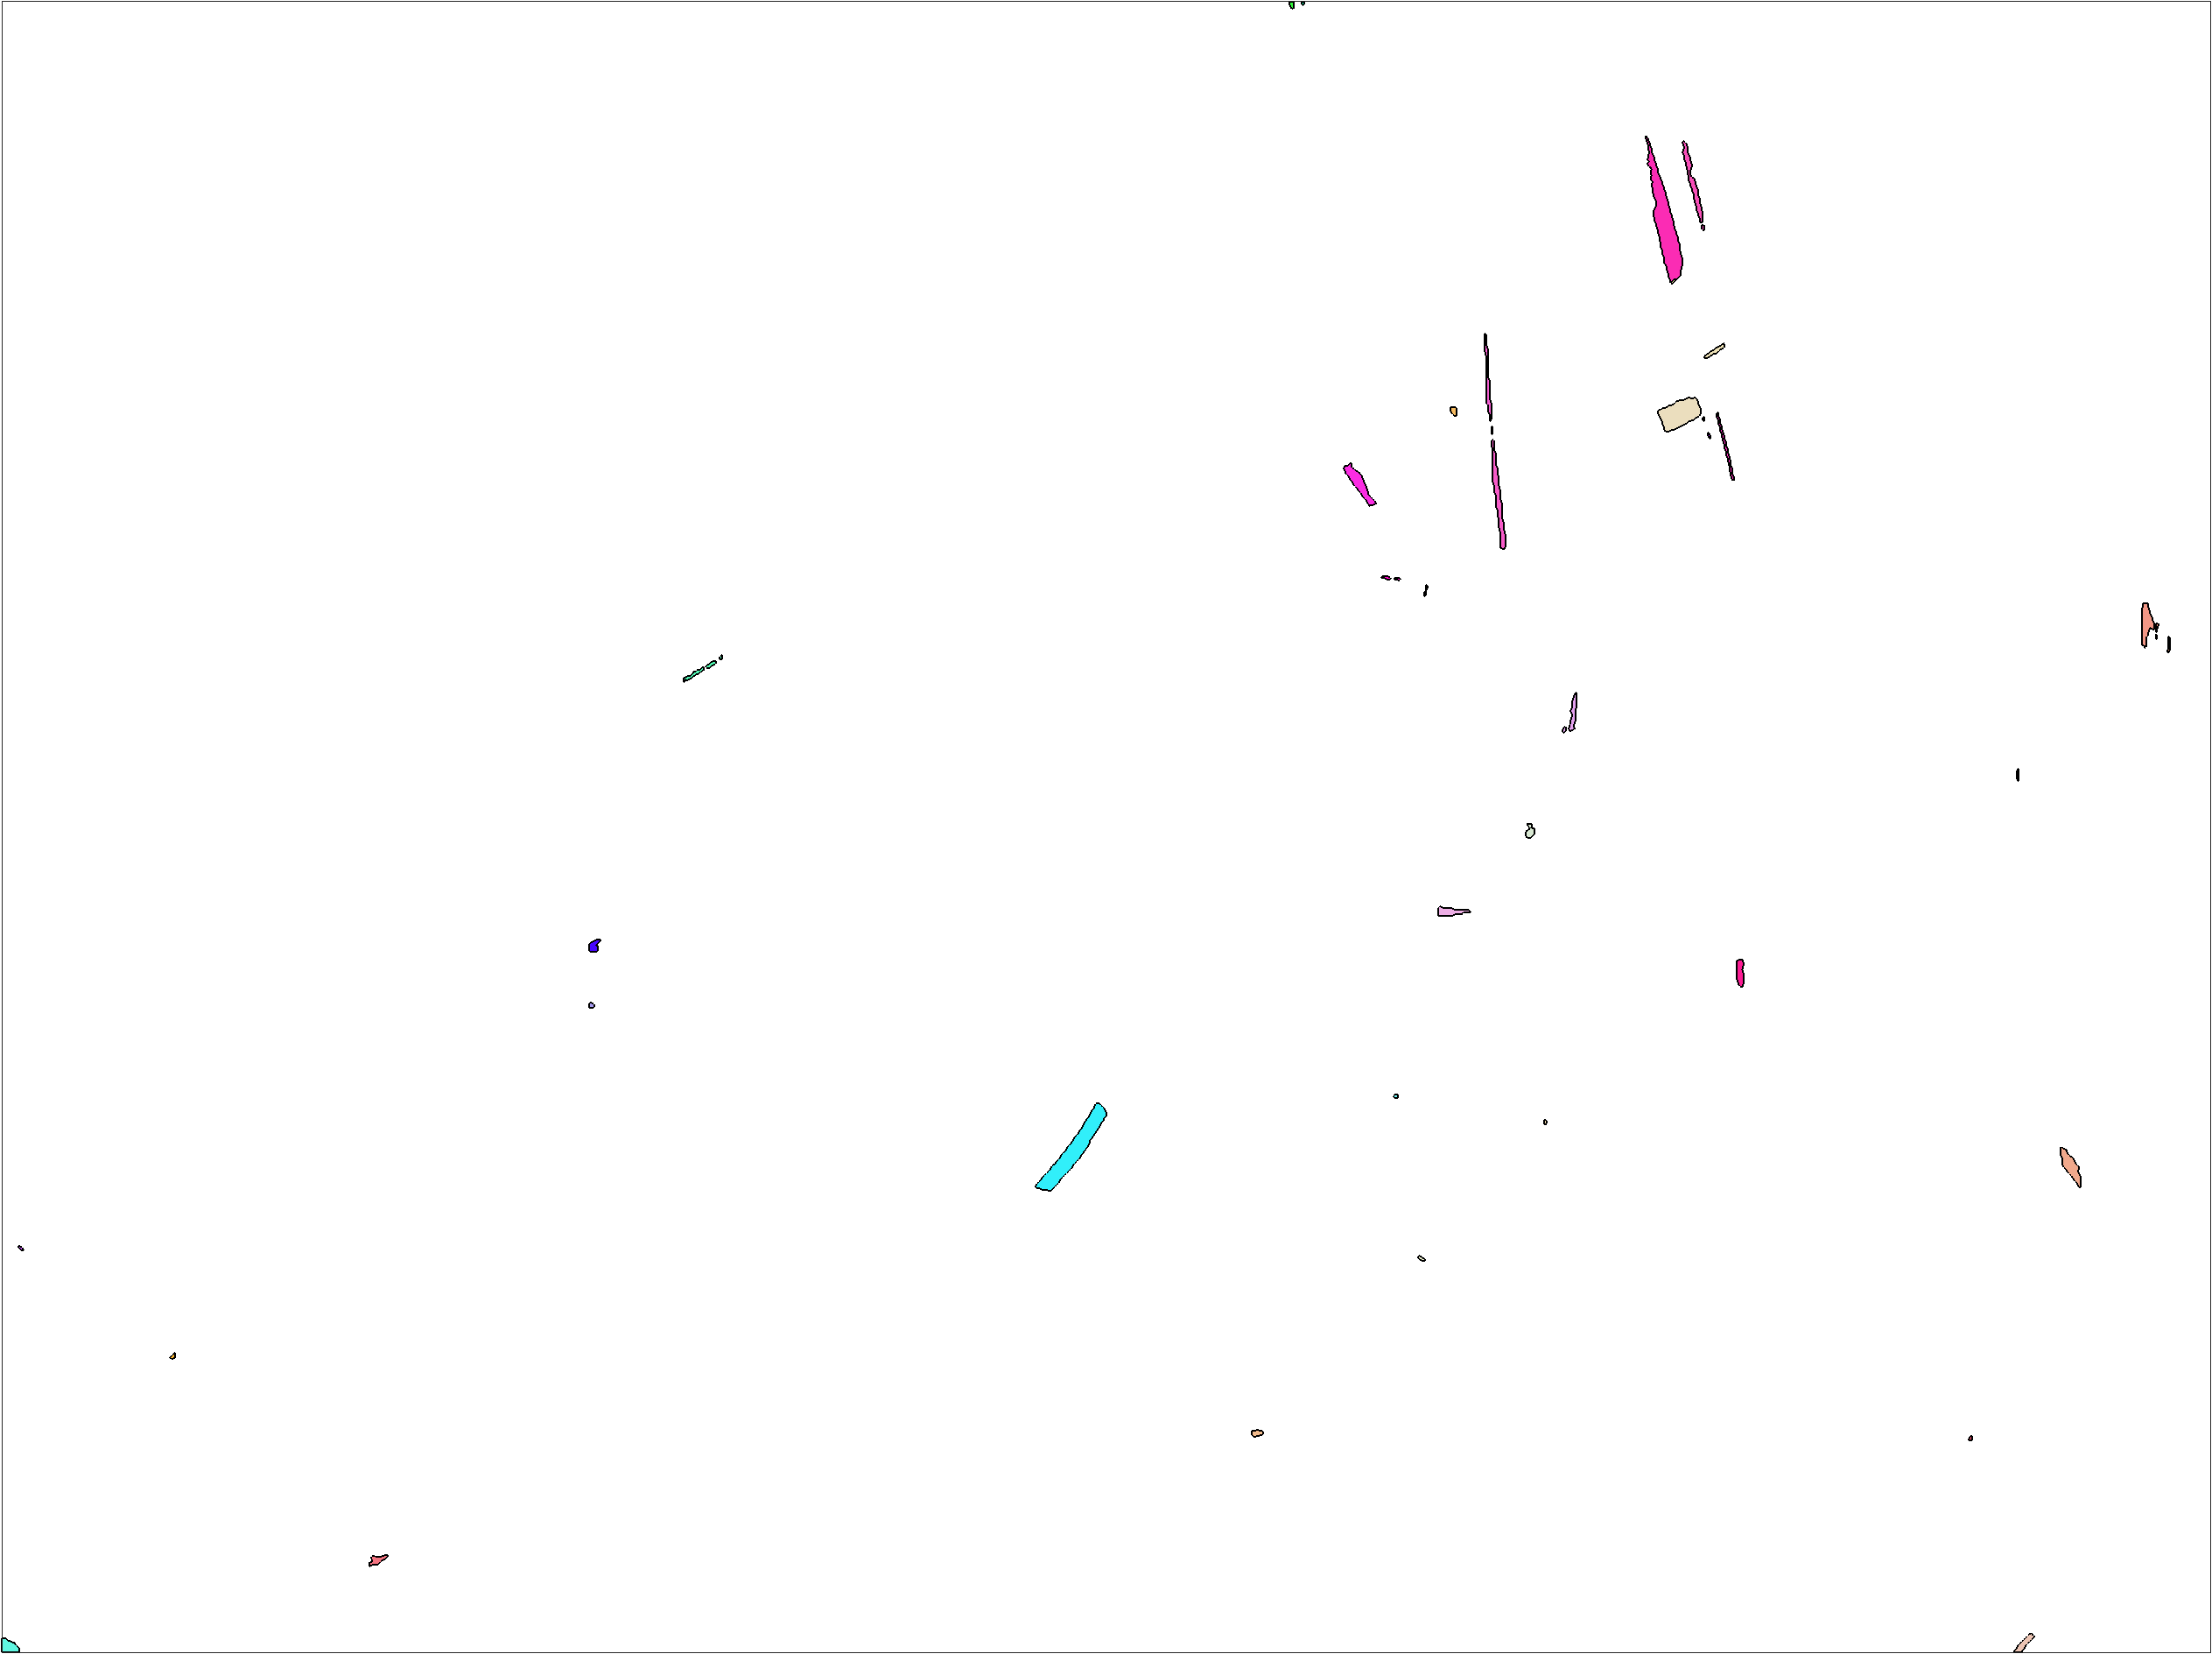
\includegraphics[width=0.3\textwidth]{pic/EpsRec_9} \quad
      \includegraphics[width=0.3\textwidth]{pic/alphaRec_4}
    \end{onlyenv}
    \begin{onlyenv}<3>
      \includegraphics[width=0.3\textwidth]{pic/gammaRec_10} \quad
      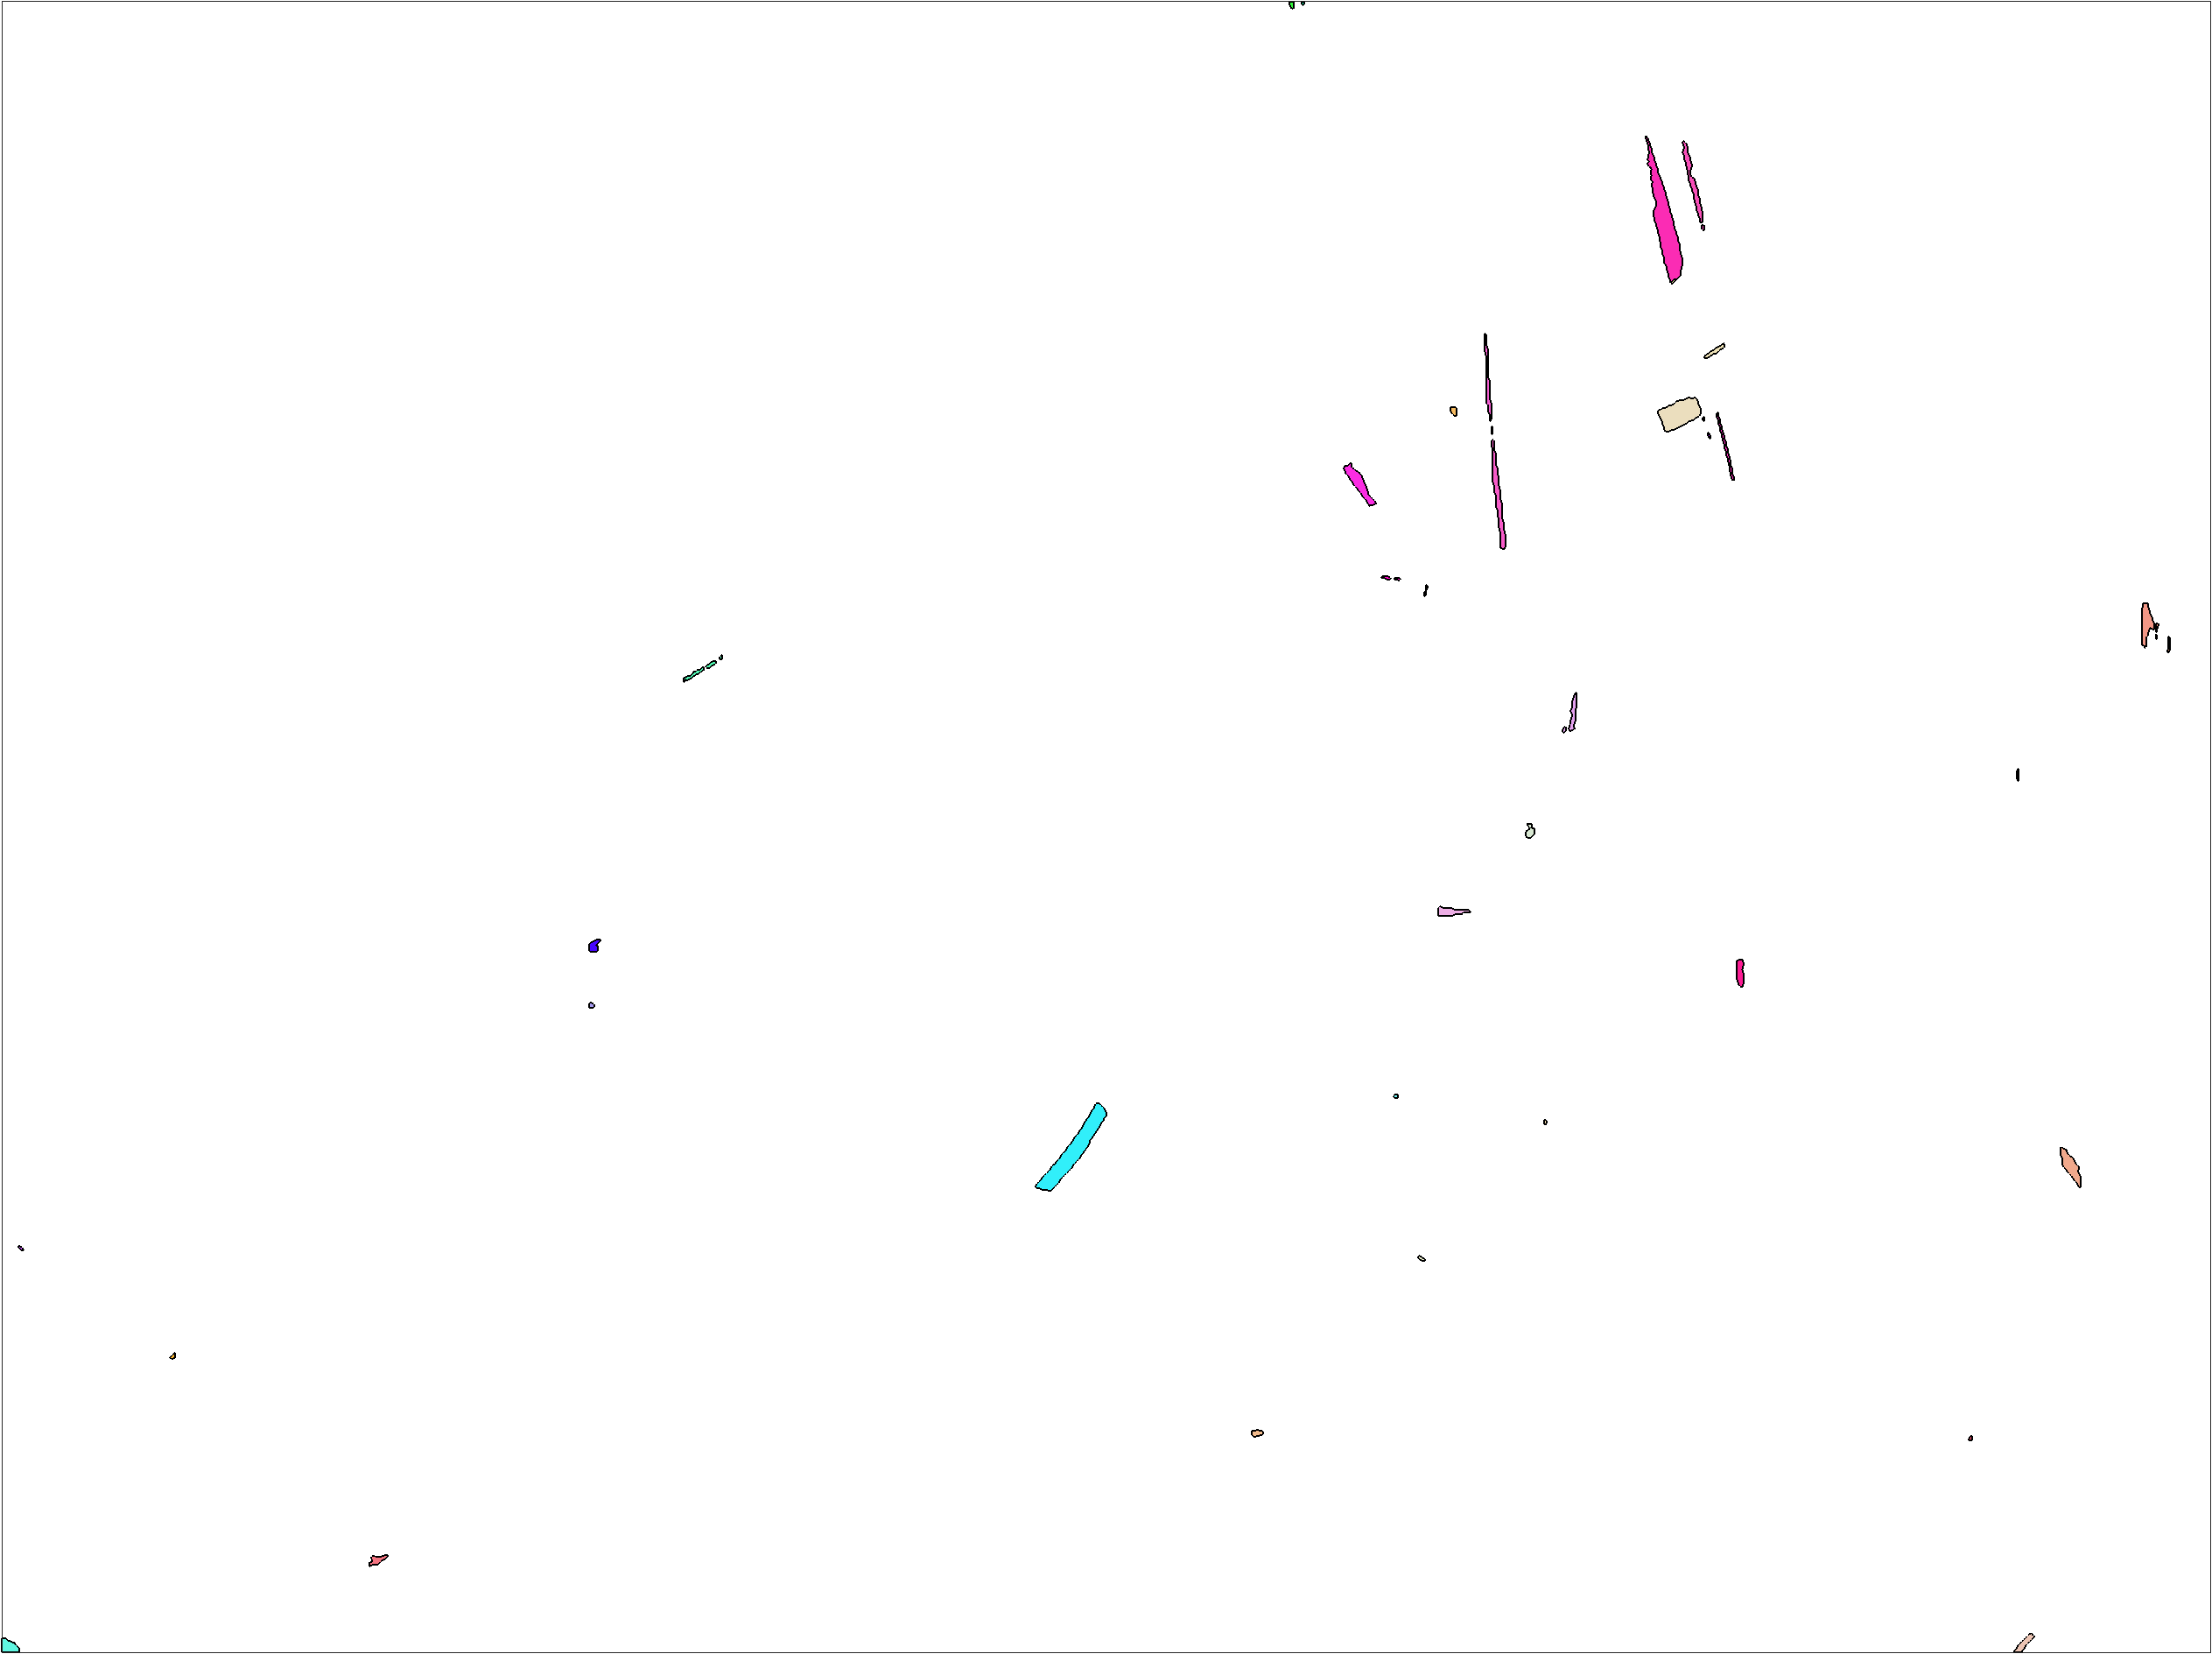
\includegraphics[width=0.3\textwidth]{pic/EpsRec_9} \quad
      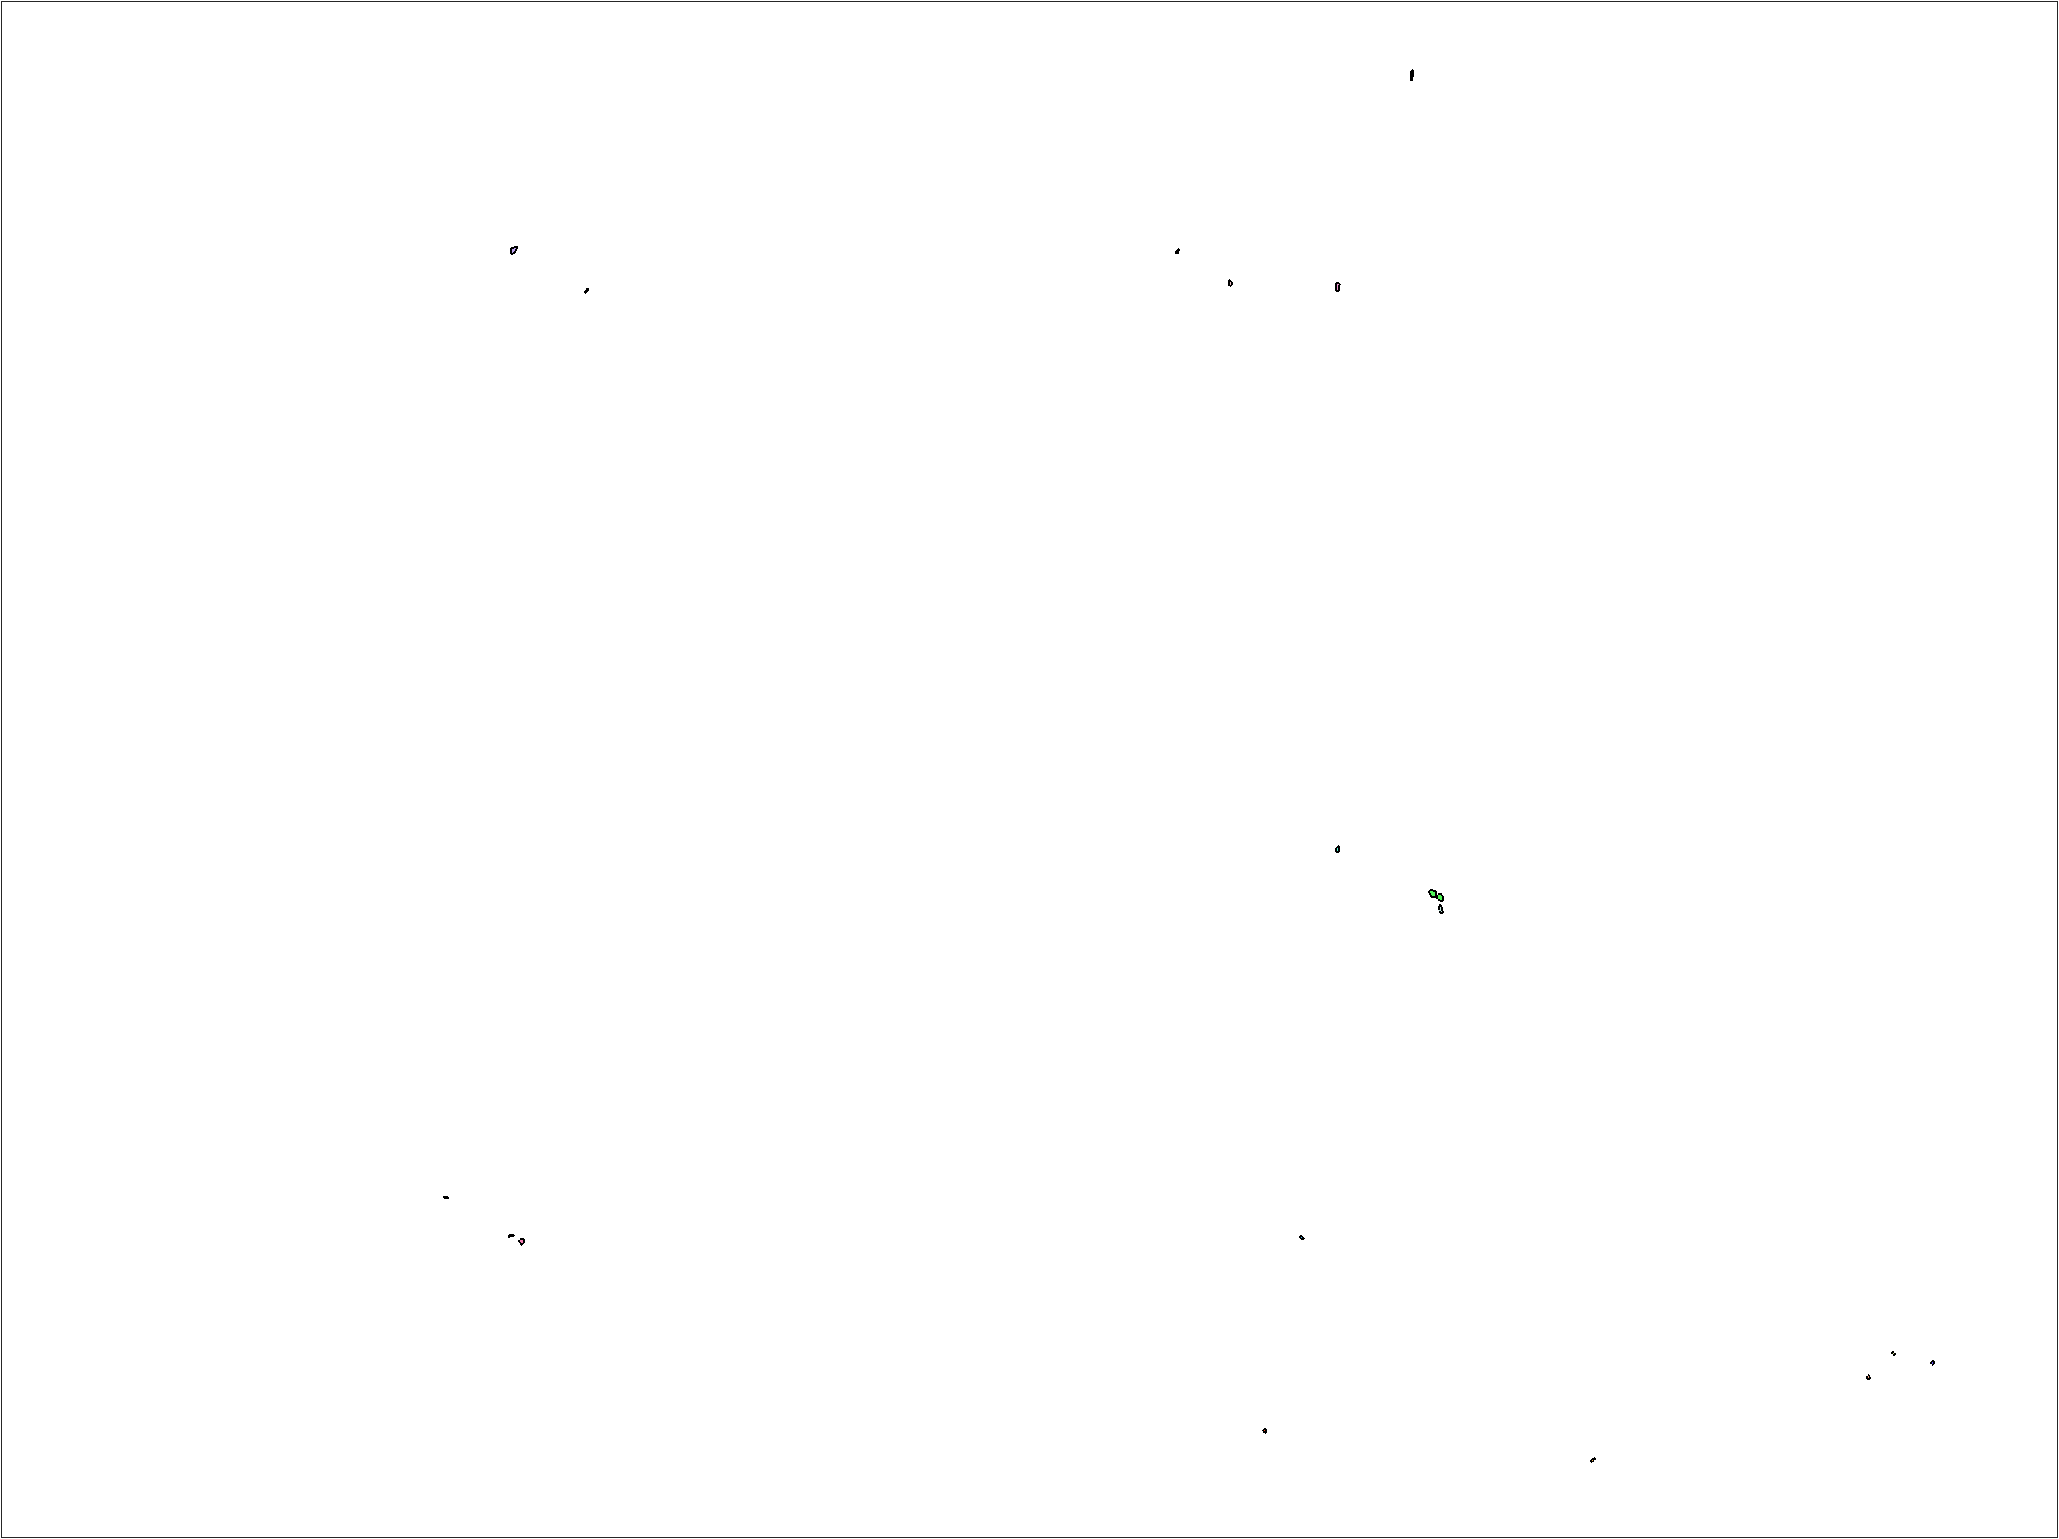
\includegraphics[width=0.3\textwidth]{pic/alphaRec_10}
    \end{onlyenv}

    \hspace{2.04cm} $\gamma$ \hspace{2.04cm} $\to$ \hspace{2.04cm}
    $\varepsilon$ \hspace{2.04cm} $\to$ \hspace{2.04cm} $\alpha'$

    \begin{onlyenv}<1>
\begin{lstlisting}[style=input]
job.mergeSimilar
\end{lstlisting}
      \vspace{-0.4cm}
    \end{onlyenv}
    \begin{onlyenv}<1>
\begin{lstlisting}[style=input]
job2 = parentGrainReconstructor(job.ebsd, job.grains)
job2.p2c = orientation.ShojiNishiyama(csGamma, csEps)
\end{lstlisting}
    \end{onlyenv}
    \begin{onlyenv}<2>
\begin{lstlisting}[style=input]
job2 = parentGrainReconstructor(job.ebsd, job.grains)
job2.p2c = orientation.ShojiNishiyama(csGamma, csEps)
job2.calcVariantGraph
job2.clusterVariantGraph
job2.calcParentFromVote
\end{lstlisting}
    \end{onlyenv}
    \begin{onlyenv}<3>
\begin{lstlisting}[style=input]
job3 = parentGrainReconstructor(job2.ebsd, job2.grains)
job3.p2c = job.p2c * job2.p2c
\end{lstlisting}
\vspace{-0.4cm}
\begin{lstlisting}[style=input]
job3.calcVariantGraph
job3.clusterVariantGraph
job3.calcParentFromVote
\end{lstlisting}
    \end{onlyenv}
    \begin{onlyenv}<1>
      \vspace{-0.4cm}
\begin{lstlisting}[style=output]
job2 = parentGrainReconstructor (show methods, plot)

 phase   mineral  symmetry  grains  area  reconstructed
 parent  gamma    m-3m      469     68%   0%
 child   epsilon  6/mmm     1010    32%

 OR: (111)||(0001)  [10-1]||[2-1-10]
   p2c fit: 0.45°, 1.1°, 2.1°, 5.9° (quintiles)
   c2c fit: 0.67°, 1.2°, 2°, 6.4° (quintiles)
\end{lstlisting}
        \end{onlyenv}
              \vspace{-0.4cm}
%         \begin{onlyenv}<2>
% \begin{lstlisting}[style=output]
% job2 = parentGrainReconstructor

%  phase   mineral  symmetry  grains  area  reconstructed
%  parent  gamma    m-3m      1250    97%   77%
%  child   epsilon  6/mmm     229     2.5%

%  OR: (111)||(0001)  [10-1]||[2-1-10]
%    p2c fit: 3°, 4°, 5.7°, 10° (quintiles)
%    c2c fit: 0.87°, 1.6°, 2.2°, 5.6° (quintiles)
% \end{lstlisting}
%         \end{onlyenv}

        \begin{onlyenv}<2>
\begin{lstlisting}[style=output]
job2 = parentGrainReconstructor

 phase   mineral  symmetry  grains  area   reconstructed
 parent  gamma    m-3m      1432    100%   95%
 child   epsilon  6/mmm     47      0.23%

 OR: (111)||(0001)  [10-1]||[2-1-10]
   p2c fit: 7.6°, 9.6°, 11°, 33° (quintiles)
   c2c fit: 1.1°, 1.1°, 1.1°, 1.1° (quintiles)
\end{lstlisting}
        \end{onlyenv}

                \begin{onlyenv}<3>
\begin{lstlisting}[style=output]
job3 = parentGrainReconstructor

 phase   mineral  symmetry  grains  area   reconstructed
 parent  gamma    m-3m      1432    100%   0%
 child   alphaP   m-3m      197     0.27%

 OR: (111)||(110)  [-101]||[1-11]
   p2c fit: 2.2°, 3.4°, 4.3°, 5.2° (quintiles)
   c2c fit: 3.3°, 3.4°, 3.6°, 4.3° (quintiles)
\end{lstlisting}
        \end{onlyenv}

  \end{overlayarea}

\end{frame}

\begin{frame}[fragile]
  \frametitle{Parent Grain Reconstruction}

  \begin{columns}
    \begin{column}{0.5 \textwidth}
      \begin{overlayarea}{\textwidth}{0.8\textheight}

        a child orientation $\mathtt{ori}_{\mathtt{C}}$ may originate from
        different parent orientations
        \begin{equation*}
          \mathtt{ori}_{\mathtt{P}} =
          \mathtt{sym}_{\mathtt{P}} * \mathtt{p2c}^{-1} * \mathtt{sym}_{\mathtt{C}} * \mathtt{ori}_{\mathtt{C}} 
        \end{equation*}

        \structure{Challenges:}
        \begin{itemize}
        \item pairs of very closely oriented variants
        \item austenite twins share many variants
        \end{itemize}

        \bigskip
        
        \begin{onlyenv}<2> \structure{General Approach:} For each child grain
          select one of the parent variants such that

          \medskip
      
          \begin{itemize}
          \item the parent orientations form clusters of similar orientations.
          \item the clusters have a reasonable morphology
            % \item The morphology of a high-temperature parent phase
            %   microstructure, typically comprising equiaxed grains.
            % \item An annealing twin structure exhibiting a boundary
            %   morphology typical of coherent $\Sigma 3$ related twin
            %   boundaries \cite{Mahajan1996}.
          \end{itemize}
        \end{onlyenv}

      \end{overlayarea}
    \end{column}
    \begin{column}{0.45 \textwidth}
      \begin{overlayarea}{\textwidth}{0.8\textheight}
        \vspace{-1.5cm}
        \begin{onlyenv}<1->
          \includegraphics[width=\textwidth]{pic/childgrains.png}
        \end{onlyenv}
        
        \begin{onlyenv}<2>
          \includegraphics[width=\textwidth]{pic/parentgrains.png}
        \end{onlyenv}
        
        
      \end{overlayarea}
     
    \end{column}
  \end{columns}
  
\end{frame}






\begin{frame}
  \frametitle{Comparison of the Graph and the Voting Based Approach}

  \begin{columns}[T,onlytextwidth]
    \begin{column}{0.48\textwidth}
      \vspace{-0.3cm}
      \structure{voting based approach}
      \begin{itemize}
        \setlength\itemsep{0.7em}
      \item considers all matching pairs of potential parent orientations        
      \item directly yields the parent orientation
      \item different potential solutions
      \item each child grain decides for itself      
      \end{itemize}

      \bigskip
      
      \structure{graph based approach}
      \begin{itemize}
        \setlength\itemsep{0.7em}
      \item considers higher order neighbors
      \item only best match counts
      \item no direct parent orientation
      \item may form inconsistent clusters
      \end{itemize}
    \end{column}
    \begin{column}{0.48\textwidth}
            \vspace{-0.4cm}
      \begin{overlayarea}{\textwidth}{0.8\textheight}
        \only<1>{%
          


\tikzset{every picture/.style={line width=0.75pt}} %set default line width to 0.75pt        

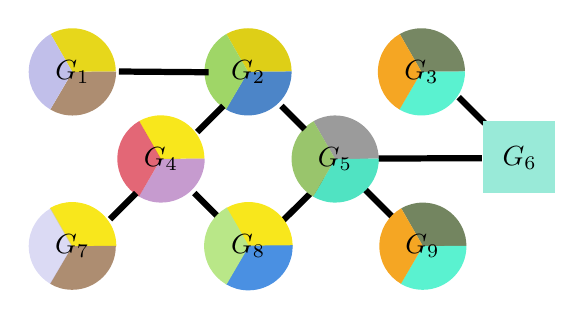
\begin{tikzpicture}[x=0.75pt,y=0.75pt,yscale=-0.7,xscale=0.7]
%uncomment if require: \path (0,1438); %set diagram left start at 0, and has height of 1438

%Straight Lines [id:da4750966694185179] 
\draw [color={rgb, 255:red, 0; green, 0; blue, 0 }  ,draw opacity=1 ][line width=2.25]    (252,1020) -- (272,1040) ;
%Straight Lines [id:da5150276886008835] 
\draw [color={rgb, 255:red, 0; green, 0; blue, 0 }  ,draw opacity=1 ][line width=2.25]    (312,1040) -- (342,1010.31) ;
%Straight Lines [id:da4895817670375473] 
\draw [color={rgb, 255:red, 0; green, 0; blue, 0 }  ,draw opacity=1 ][line width=2.25]    (362,1010) -- (392,1040) ;
%Straight Lines [id:da8896491664010189] 
\draw [color={rgb, 255:red, 0; green, 0; blue, 0 }  ,draw opacity=1 ][line width=2.25]    (378.8,996.26) -- (450,996) ;
%Shape: Pie [id:dp15959605123169607] 
\draw  [draw opacity=0][fill={rgb, 255:red, 248; green, 231; blue, 28 }  ,fill opacity=1 ] (214.1,970.48) .. controls (218.49,967.96) and (223.58,966.52) .. (229,966.52) .. controls (245.48,966.52) and (258.86,979.81) .. (259,996.26) -- (229,996.52) -- cycle ;
%Shape: Pie [id:dp7541674422286544] 
\draw  [draw opacity=0][fill={rgb, 255:red, 170; green, 106; blue, 183 }  ,fill opacity=0.67 ] (259.19,996.28) .. controls (259.19,996.37) and (259.19,996.47) .. (259.19,996.57) .. controls (259.19,1013.14) and (245.76,1026.57) .. (229.19,1026.57) .. controls (223.62,1026.57) and (218.39,1025.05) .. (213.92,1022.4) -- (229.19,996.57) -- cycle ;
%Shape: Pie [id:dp5711882691598997] 
\draw  [draw opacity=0][fill={rgb, 255:red, 208; green, 2; blue, 27 }  ,fill opacity=0.6 ] (213.92,1022.4) .. controls (205.03,1017.19) and (199.06,1007.54) .. (199.06,996.49) .. controls (199.06,985.37) and (205.11,975.66) .. (214.1,970.48) -- (229.06,996.49) -- cycle ;
%Shape: Pie [id:dp06487384610910718] 
\draw  [draw opacity=0][fill={rgb, 255:red, 155; green, 155; blue, 155 }  ,fill opacity=1 ] (334.04,970.56) .. controls (338.43,968.04) and (343.52,966.6) .. (348.94,966.6) .. controls (365.42,966.6) and (378.8,979.89) .. (378.94,996.34) -- (348.94,996.6) -- cycle ;
%Shape: Pie [id:dp7524611065236799] 
\draw  [draw opacity=0][fill={rgb, 255:red, 80; green, 227; blue, 194 }  ,fill opacity=1 ] (379,996.28) .. controls (379,996.37) and (379,996.47) .. (379,996.57) .. controls (379,1013.14) and (365.57,1026.57) .. (349,1026.57) .. controls (343.42,1026.57) and (338.2,1025.05) .. (333.73,1022.4) -- (349,996.57) -- cycle ;
%Shape: Pie [id:dp59207049369319] 
\draw  [draw opacity=0][fill={rgb, 255:red, 153; green, 197; blue, 108 }  ,fill opacity=1 ] (333.86,1022.48) .. controls (324.97,1017.27) and (319,1007.62) .. (319,996.57) .. controls (319,985.45) and (325.05,975.74) .. (334.04,970.56) -- (349,996.57) -- cycle ;
%Shape: Pie [id:dp22947674130855522] 
\draw  [draw opacity=0][fill={rgb, 255:red, 34; green, 61; blue, 3 }  ,fill opacity=0.63 ] (394.43,1030.54) .. controls (398.82,1028.02) and (403.91,1026.58) .. (409.33,1026.58) .. controls (425.81,1026.58) and (439.18,1039.87) .. (439.33,1056.31) -- (409.33,1056.58) -- cycle ;
%Shape: Pie [id:dp2835887548099052] 
\draw  [draw opacity=0][fill={rgb, 255:red, 90; green, 242; blue, 208 }  ,fill opacity=1 ] (439.33,1056.31) .. controls (439.33,1056.41) and (439.33,1056.51) .. (439.33,1056.6) .. controls (439.33,1073.17) and (425.9,1086.6) .. (409.33,1086.6) .. controls (403.75,1086.6) and (398.53,1085.08) .. (394.06,1082.43) -- (409.33,1056.6) -- cycle ;
%Shape: Pie [id:dp13060561720498276] 
\draw  [draw opacity=0][fill={rgb, 255:red, 245; green, 166; blue, 35 }  ,fill opacity=1 ] (394.25,1082.45) .. controls (385.36,1077.24) and (379.39,1067.59) .. (379.39,1056.54) .. controls (379.39,1045.42) and (385.44,1035.72) .. (394.43,1030.54) -- (409.39,1056.54) -- cycle ;
%Shape: Pie [id:dp25936104896268675] 
\draw  [color={rgb, 255:red, 248; green, 231; blue, 28 }  ,draw opacity=1 ][fill={rgb, 255:red, 248; green, 231; blue, 28 }  ,fill opacity=1 ] (274.43,1030.54) .. controls (278.82,1028.02) and (283.91,1026.58) .. (289.33,1026.58) .. controls (305.81,1026.58) and (319.18,1039.87) .. (319.33,1056.31) -- (289.33,1056.58) -- cycle ;
%Shape: Pie [id:dp18697217704809055] 
\draw  [color={rgb, 255:red, 74; green, 144; blue, 226 }  ,draw opacity=1 ][fill={rgb, 255:red, 74; green, 144; blue, 226 }  ,fill opacity=1 ] (319.33,1056.31) .. controls (319.33,1056.41) and (319.33,1056.51) .. (319.33,1056.6) .. controls (319.33,1073.17) and (305.9,1086.6) .. (289.33,1086.6) .. controls (283.75,1086.6) and (278.53,1085.08) .. (274.06,1082.43) -- (289.33,1056.6) -- cycle ;
%Shape: Pie [id:dp8724690316630832] 
\draw  [color={rgb, 255:red, 185; green, 231; blue, 136 }  ,draw opacity=1 ][fill={rgb, 255:red, 185; green, 231; blue, 136 }  ,fill opacity=1 ] (274.06,1082.43) .. controls (265.17,1077.22) and (259.19,1067.57) .. (259.19,1056.52) .. controls (259.19,1045.4) and (265.24,1035.7) .. (274.23,1030.52) -- (289.19,1056.52) -- cycle ;
%Shape: Pie [id:dp4015988811299751] 
\draw  [draw opacity=0][fill={rgb, 255:red, 34; green, 61; blue, 3 }  ,fill opacity=0.62 ] (393.43,910.56) .. controls (397.82,908.04) and (402.91,906.6) .. (408.33,906.6) .. controls (424.81,906.6) and (438.19,919.89) .. (438.33,936.34) -- (408.33,936.6) -- cycle ;
%Shape: Pie [id:dp6392181041712679] 
\draw  [draw opacity=0][fill={rgb, 255:red, 90; green, 242; blue, 208 }  ,fill opacity=1 ] (438.33,936.31) .. controls (438.33,936.41) and (438.33,936.51) .. (438.33,936.6) .. controls (438.33,953.17) and (424.9,966.6) .. (408.33,966.6) .. controls (402.75,966.6) and (397.53,965.08) .. (393.06,962.43) -- (408.33,936.6) -- cycle ;
%Shape: Pie [id:dp04268417484462428] 
\draw  [draw opacity=0][fill={rgb, 255:red, 245; green, 166; blue, 35 }  ,fill opacity=1 ] (393.25,962.48) .. controls (384.36,957.27) and (378.39,947.62) .. (378.39,936.57) .. controls (378.39,925.45) and (384.44,915.74) .. (393.43,910.56) -- (408.39,936.57) -- cycle ;
%Shape: Pie [id:dp2303075286248355] 
\draw  [draw opacity=0][fill={rgb, 255:red, 222; green, 207; blue, 23 }  ,fill opacity=1 ] (274.1,910.54) .. controls (278.49,908.02) and (283.58,906.58) .. (289,906.58) .. controls (305.48,906.58) and (318.86,919.87) .. (319,936.31) -- (289,936.58) -- cycle ;
%Shape: Pie [id:dp8616807370257602] 
\draw  [draw opacity=0][fill={rgb, 255:red, 76; green, 133; blue, 200 }  ,fill opacity=1 ] (319,936.31) .. controls (319,936.41) and (319,936.51) .. (319,936.6) .. controls (319,953.17) and (305.57,966.6) .. (289,966.6) .. controls (283.42,966.6) and (278.2,965.08) .. (273.73,962.43) -- (289,936.6) -- cycle ;
%Shape: Pie [id:dp043769946944892446] 
\draw  [draw opacity=0][fill={rgb, 255:red, 159; green, 214; blue, 103 }  ,fill opacity=1 ] (273.92,962.45) .. controls (265.03,957.24) and (259.06,947.59) .. (259.06,936.54) .. controls (259.06,925.42) and (265.11,915.72) .. (274.1,910.54) -- (289.06,936.54) -- cycle ;
%Shape: Pie [id:dp5705398645606532] 
\draw  [draw opacity=0][fill={rgb, 255:red, 231; green, 215; blue, 27 }  ,fill opacity=1 ] (153.1,910.56) .. controls (157.49,908.04) and (162.58,906.6) .. (168,906.6) .. controls (184.48,906.6) and (197.86,919.89) .. (198,936.34) -- (168,936.6) -- cycle ;
%Shape: Pie [id:dp7072389331728437] 
\draw  [draw opacity=0][fill={rgb, 255:red, 173; green, 141; blue, 113 }  ,fill opacity=1 ] (198.19,936.36) .. controls (198.19,936.45) and (198.19,936.55) .. (198.19,936.65) .. controls (198.19,953.22) and (184.76,966.65) .. (168.19,966.65) .. controls (162.62,966.65) and (157.39,965.13) .. (152.92,962.48) -- (168.19,936.65) -- cycle ;
%Shape: Pie [id:dp8158973417554063] 
\draw  [draw opacity=0][fill={rgb, 255:red, 193; green, 191; blue, 234 }  ,fill opacity=1 ][line width=0.75]  (152.92,962.48) .. controls (144.03,957.27) and (138.06,947.62) .. (138.06,936.57) .. controls (138.06,925.45) and (144.11,915.74) .. (153.1,910.56) -- (168.06,936.57) -- cycle ;
%Shape: Pie [id:dp3241766948162095] 
\draw  [color={rgb, 255:red, 248; green, 231; blue, 28 }  ,draw opacity=1 ][fill={rgb, 255:red, 248; green, 231; blue, 28 }  ,fill opacity=1 ] (153.1,1030.56) .. controls (157.49,1028.04) and (162.58,1026.6) .. (168,1026.6) .. controls (184.48,1026.6) and (197.86,1039.89) .. (198,1056.34) -- (168,1056.6) -- cycle ;
%Shape: Pie [id:dp47660672298161044] 
\draw  [draw opacity=0][fill={rgb, 255:red, 173; green, 141; blue, 113 }  ,fill opacity=1 ] (198,1056.31) .. controls (198,1056.41) and (198,1056.51) .. (198,1056.6) .. controls (198,1073.17) and (184.57,1086.6) .. (168,1086.6) .. controls (162.42,1086.6) and (157.2,1085.08) .. (152.73,1082.43) -- (168,1056.6) -- cycle ;
%Shape: Pie [id:dp37127154690899333] 
\draw  [draw opacity=0][fill={rgb, 255:red, 195; green, 193; blue, 236 }  ,fill opacity=0.6 ] (152.92,1082.48) .. controls (144.03,1077.27) and (138.06,1067.62) .. (138.06,1056.57) .. controls (138.06,1045.45) and (144.11,1035.74) .. (153.1,1030.56) -- (168.06,1056.57) -- cycle ;
%Straight Lines [id:da15510273107339523] 
\draw [color={rgb, 255:red, 0; green, 0; blue, 0 }  ,draw opacity=1 ][line width=2.25]    (194,1038) -- (212,1020) ;
%Straight Lines [id:da942983095461597] 
\draw [color={rgb, 255:red, 0; green, 0; blue, 0 }  ,draw opacity=1 ][line width=2.25]    (254,978) -- (272,960) ;
%Straight Lines [id:da9752661210821294] 
\draw [color={rgb, 255:red, 0; green, 0; blue, 0 }  ,draw opacity=1 ][line width=2.25]    (312,960) -- (328,976) ;
%Straight Lines [id:da36779824965264907] 
\draw [color={rgb, 255:red, 0; green, 0; blue, 0 }  ,draw opacity=1 ][line width=2.25]    (434,954) -- (452,972) ;
%Straight Lines [id:da18311590393557386] 
\draw [color={rgb, 255:red, 0; green, 0; blue, 0 }  ,draw opacity=1 ][line width=2.25]    (200.19,936.36) -- (261.89,936.87) ;
%Shape: Square [id:dp6948642438111272] 
\draw  [draw opacity=0][fill={rgb, 255:red, 153; green, 234; blue, 216 }  ,fill opacity=1 ] (450.5,970.5) -- (500,970.5) -- (500,1020) -- (450.5,1020) -- cycle ;

% Text Node
\draw (408.39,936.57) node   [align=left] {$\displaystyle G_{3}$};
% Text Node
\draw (168,1056.6) node   [align=left] {$\displaystyle G_{7}$};
% Text Node
\draw (348.81,996.52) node   [align=left] {$\displaystyle G_{5}$};
% Text Node
\draw (289.19,1056.52) node   [align=left] {$\displaystyle G_{8}$};
% Text Node
\draw (476,996) node   [align=left] {$\displaystyle G_{6}$};
% Text Node
\draw (229,996.52) node   [align=left] {$\displaystyle G_{4}$};
% Text Node
\draw (289.06,936.54) node   [align=left] {$\displaystyle G_{2}$};
% Text Node
\draw (168.19,936.65) node  [font=\normalsize] [align=left] {$\displaystyle G_{1}$};
% Text Node
\draw (409,1056.48) node   [align=left] {$\displaystyle G_{9}$};


\end{tikzpicture}

        \bigskip
        \bigskip
        
        \input{tikz/voting1.tex}
        }%
      \only<2>{%
        \input{tikz/gg1.tex}
        
        


\tikzset{every picture/.style={line width=0.75pt}} %set default line width to 0.75pt        

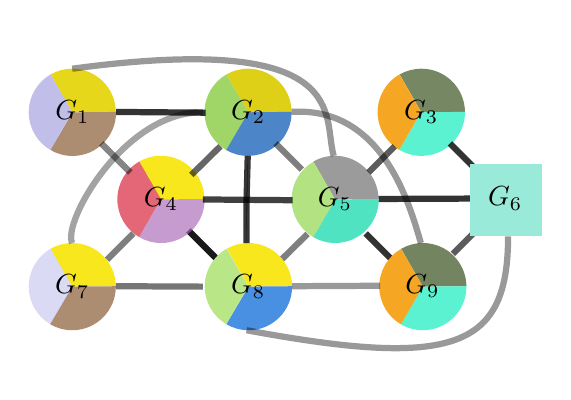
\begin{tikzpicture}[x=0.75pt,y=0.75pt,yscale=-0.7,xscale=0.7]
%uncomment if require: \path (0,1438); %set diagram left start at 0, and has height of 1438

%Straight Lines [id:da4186367162458817] 
\draw [color={rgb, 255:red, 0; green, 0; blue, 0 }  ,draw opacity=0.9 ][line width=2.25]    (248,1248) -- (270,1270) ;
%Straight Lines [id:da08988239364957362] 
\draw [color={rgb, 255:red, 0; green, 0; blue, 0 }  ,draw opacity=0.5 ][line width=2.25]    (310,1270) -- (330,1250.31) ;
%Straight Lines [id:da562224740054299] 
\draw [color={rgb, 255:red, 0; green, 0; blue, 0 }  ,draw opacity=0.8 ][line width=2.25]    (370,1250) -- (400,1280) ;
%Straight Lines [id:da5154222376250446] 
\draw [color={rgb, 255:red, 0; green, 0; blue, 0 }  ,draw opacity=0.8 ][line width=2.25]    (378.8,1226.26) -- (442,1226) ;
%Shape: Pie [id:dp22862520376005735] 
\draw  [draw opacity=0][fill={rgb, 255:red, 248; green, 231; blue, 28 }  ,fill opacity=1 ] (214.1,1200.48) .. controls (218.49,1197.96) and (223.58,1196.52) .. (229,1196.52) .. controls (245.48,1196.52) and (258.86,1209.81) .. (259,1226.26) -- (229,1226.52) -- cycle ;
%Shape: Pie [id:dp8772577465973821] 
\draw  [draw opacity=0][fill={rgb, 255:red, 170; green, 106; blue, 183 }  ,fill opacity=0.67 ] (259.19,1226.28) .. controls (259.19,1226.37) and (259.19,1226.47) .. (259.19,1226.57) .. controls (259.19,1243.14) and (245.76,1256.57) .. (229.19,1256.57) .. controls (223.62,1256.57) and (218.39,1255.05) .. (213.92,1252.4) -- (229.19,1226.57) -- cycle ;
%Shape: Pie [id:dp1897340912962322] 
\draw  [draw opacity=0][fill={rgb, 255:red, 208; green, 2; blue, 27 }  ,fill opacity=0.6 ] (213.92,1252.4) .. controls (205.03,1247.19) and (199.06,1237.54) .. (199.06,1226.49) .. controls (199.06,1215.37) and (205.11,1205.66) .. (214.1,1200.48) -- (229.06,1226.49) -- cycle ;
%Shape: Pie [id:dp5352410492568669] 
\draw  [draw opacity=0][fill={rgb, 255:red, 155; green, 155; blue, 155 }  ,fill opacity=1 ] (333.9,1200.48) .. controls (338.29,1197.96) and (343.38,1196.52) .. (348.81,1196.52) .. controls (365.29,1196.52) and (378.66,1209.81) .. (378.8,1226.26) -- (348.81,1226.52) -- cycle ;
%Shape: Pie [id:dp711098439811789] 
\draw  [draw opacity=0][fill={rgb, 255:red, 80; green, 227; blue, 194 }  ,fill opacity=1 ] (379,1226.28) .. controls (379,1226.37) and (379,1226.47) .. (379,1226.57) .. controls (379,1243.14) and (365.57,1256.57) .. (349,1256.57) .. controls (343.42,1256.57) and (338.2,1255.05) .. (333.73,1252.4) -- (349,1226.57) -- cycle ;
%Shape: Pie [id:dp7438737756485665] 
\draw  [draw opacity=0][fill={rgb, 255:red, 178; green, 226; blue, 130 }  ,fill opacity=1 ] (333.86,1252.48) .. controls (324.97,1247.27) and (319,1237.62) .. (319,1226.57) .. controls (319,1215.45) and (325.05,1205.74) .. (334.04,1200.56) -- (349,1226.57) -- cycle ;
%Shape: Pie [id:dp4950401144432839] 
\draw  [draw opacity=0][fill={rgb, 255:red, 34; green, 61; blue, 3 }  ,fill opacity=0.63 ] (394.43,1260.54) .. controls (398.82,1258.02) and (403.91,1256.58) .. (409.33,1256.58) .. controls (425.81,1256.58) and (439.18,1269.87) .. (439.33,1286.31) -- (409.33,1286.58) -- cycle ;
%Shape: Pie [id:dp32846163458006306] 
\draw  [draw opacity=0][fill={rgb, 255:red, 90; green, 242; blue, 208 }  ,fill opacity=1 ] (439.33,1286.31) .. controls (439.33,1286.41) and (439.33,1286.51) .. (439.33,1286.6) .. controls (439.33,1303.17) and (425.9,1316.6) .. (409.33,1316.6) .. controls (403.75,1316.6) and (398.53,1315.08) .. (394.06,1312.43) -- (409.33,1286.6) -- cycle ;
%Shape: Pie [id:dp6513356609327752] 
\draw  [draw opacity=0][fill={rgb, 255:red, 245; green, 166; blue, 35 }  ,fill opacity=1 ] (394.19,1312.51) .. controls (385.3,1307.3) and (379.33,1297.65) .. (379.33,1286.6) .. controls (379.33,1275.48) and (385.38,1265.78) .. (394.37,1260.6) -- (409.33,1286.6) -- cycle ;
%Shape: Pie [id:dp7206062426889672] 
\draw  [draw opacity=0][fill={rgb, 255:red, 248; green, 231; blue, 28 }  ,fill opacity=1 ] (274.43,1260.54) .. controls (278.82,1258.02) and (283.91,1256.58) .. (289.33,1256.58) .. controls (305.81,1256.58) and (319.18,1269.87) .. (319.33,1286.31) -- (289.33,1286.58) -- cycle ;
%Shape: Pie [id:dp8650493341112429] 
\draw  [draw opacity=0][fill={rgb, 255:red, 74; green, 144; blue, 226 }  ,fill opacity=1 ] (319.33,1286.31) .. controls (319.33,1286.41) and (319.33,1286.51) .. (319.33,1286.6) .. controls (319.33,1303.17) and (305.9,1316.6) .. (289.33,1316.6) .. controls (283.75,1316.6) and (278.53,1315.08) .. (274.06,1312.43) -- (289.33,1286.6) -- cycle ;
%Shape: Pie [id:dp3972433808884661] 
\draw  [draw opacity=0][fill={rgb, 255:red, 185; green, 231; blue, 136 }  ,fill opacity=1 ] (274.06,1312.43) .. controls (265.17,1307.22) and (259.19,1297.57) .. (259.19,1286.52) .. controls (259.19,1275.4) and (265.24,1265.7) .. (274.23,1260.52) -- (289.19,1286.52) -- cycle ;
%Shape: Pie [id:dp14987497027583996] 
\draw  [draw opacity=0][fill={rgb, 255:red, 34; green, 61; blue, 3 }  ,fill opacity=0.62 ] (393.43,1140.56) .. controls (397.82,1138.04) and (402.91,1136.6) .. (408.33,1136.6) .. controls (424.81,1136.6) and (438.19,1149.89) .. (438.33,1166.34) -- (408.33,1166.6) -- cycle ;
%Shape: Pie [id:dp6281781916199654] 
\draw  [draw opacity=0][fill={rgb, 255:red, 90; green, 242; blue, 208 }  ,fill opacity=1 ] (438.33,1166.31) .. controls (438.33,1166.41) and (438.33,1166.51) .. (438.33,1166.6) .. controls (438.33,1183.17) and (424.9,1196.6) .. (408.33,1196.6) .. controls (402.75,1196.6) and (397.53,1195.08) .. (393.06,1192.43) -- (408.33,1166.6) -- cycle ;
%Shape: Pie [id:dp7368216785514972] 
\draw  [draw opacity=0][fill={rgb, 255:red, 245; green, 166; blue, 35 }  ,fill opacity=1 ] (393.06,1192.43) .. controls (384.17,1187.22) and (378.19,1177.57) .. (378.19,1166.52) .. controls (378.19,1155.4) and (384.24,1145.7) .. (393.23,1140.52) -- (408.19,1166.52) -- cycle ;
%Shape: Pie [id:dp27649490289378686] 
\draw  [draw opacity=0][fill={rgb, 255:red, 222; green, 207; blue, 23 }  ,fill opacity=1 ] (274.1,1140.56) .. controls (278.49,1138.04) and (283.58,1136.6) .. (289,1136.6) .. controls (305.48,1136.6) and (318.86,1149.89) .. (319,1166.34) -- (289,1166.6) -- cycle ;
%Shape: Pie [id:dp8058575634583287] 
\draw  [draw opacity=0][fill={rgb, 255:red, 76; green, 133; blue, 200 }  ,fill opacity=1 ] (319,1166.31) .. controls (319,1166.41) and (319,1166.51) .. (319,1166.6) .. controls (319,1183.17) and (305.57,1196.6) .. (289,1196.6) .. controls (283.42,1196.6) and (278.2,1195.08) .. (273.73,1192.43) -- (289,1166.6) -- cycle ;
%Shape: Pie [id:dp5685252067895206] 
\draw  [draw opacity=0][fill={rgb, 255:red, 159; green, 214; blue, 103 }  ,fill opacity=1 ] (273.92,1192.48) .. controls (265.03,1187.27) and (259.06,1177.62) .. (259.06,1166.57) .. controls (259.06,1155.45) and (265.11,1145.74) .. (274.1,1140.56) -- (289.06,1166.57) -- cycle ;
%Shape: Pie [id:dp34533858656916694] 
\draw  [draw opacity=0][fill={rgb, 255:red, 231; green, 215; blue, 27 }  ,fill opacity=1 ] (153.1,1140.56) .. controls (157.49,1138.04) and (162.58,1136.6) .. (168,1136.6) .. controls (184.48,1136.6) and (197.86,1149.89) .. (198,1166.34) -- (168,1166.6) -- cycle ;
%Shape: Pie [id:dp6381985445084128] 
\draw  [draw opacity=0][fill={rgb, 255:red, 173; green, 141; blue, 113 }  ,fill opacity=1 ] (198.19,1166.36) .. controls (198.19,1166.45) and (198.19,1166.55) .. (198.19,1166.65) .. controls (198.19,1183.22) and (184.76,1196.65) .. (168.19,1196.65) .. controls (162.62,1196.65) and (157.39,1195.13) .. (152.92,1192.48) -- (168.19,1166.65) -- cycle ;
%Shape: Pie [id:dp9772609477611058] 
\draw  [draw opacity=0][fill={rgb, 255:red, 193; green, 191; blue, 234 }  ,fill opacity=1 ][line width=0.75]  (152.92,1192.48) .. controls (144.03,1187.27) and (138.06,1177.62) .. (138.06,1166.57) .. controls (138.06,1155.45) and (144.11,1145.74) .. (153.1,1140.56) -- (168.06,1166.57) -- cycle ;
%Shape: Pie [id:dp29151881669152435] 
\draw  [draw opacity=0][fill={rgb, 255:red, 248; green, 231; blue, 28 }  ,fill opacity=1 ] (153.1,1260.56) .. controls (157.49,1258.04) and (162.58,1256.6) .. (168,1256.6) .. controls (184.48,1256.6) and (197.86,1269.89) .. (198,1286.34) -- (168,1286.6) -- cycle ;
%Shape: Pie [id:dp5832605538270472] 
\draw  [draw opacity=0][fill={rgb, 255:red, 173; green, 141; blue, 113 }  ,fill opacity=1 ] (198,1286.31) .. controls (198,1286.41) and (198,1286.51) .. (198,1286.6) .. controls (198,1303.17) and (184.57,1316.6) .. (168,1316.6) .. controls (162.42,1316.6) and (157.2,1315.08) .. (152.73,1312.43) -- (168,1286.6) -- cycle ;
%Shape: Pie [id:dp04827723823086716] 
\draw  [draw opacity=0][fill={rgb, 255:red, 195; green, 193; blue, 236 }  ,fill opacity=0.6 ] (152.92,1312.48) .. controls (144.03,1307.27) and (138.06,1297.62) .. (138.06,1286.57) .. controls (138.06,1275.45) and (144.11,1265.74) .. (153.1,1260.56) -- (168.06,1286.57) -- cycle ;
%Straight Lines [id:da1744544159777348] 
\draw [color={rgb, 255:red, 0; green, 0; blue, 0 }  ,draw opacity=0.5 ][line width=2.25]    (192,1268) -- (210,1250) ;
%Straight Lines [id:da03935827821553706] 
\draw [color={rgb, 255:red, 0; green, 0; blue, 0 }  ,draw opacity=0.6 ][line width=2.25]    (250,1209.69) -- (270,1190) ;
%Straight Lines [id:da3827572200791203] 
\draw [color={rgb, 255:red, 0; green, 0; blue, 0 }  ,draw opacity=0.5 ][line width=2.25]    (308,1188) -- (326,1206) ;
%Straight Lines [id:da43054867062761004] 
\draw [color={rgb, 255:red, 0; green, 0; blue, 0 }  ,draw opacity=0.8 ][line width=2.25]    (428,1188) -- (450,1210) ;
%Straight Lines [id:da8030640791722374] 
\draw [color={rgb, 255:red, 0; green, 0; blue, 0 }  ,draw opacity=0.8 ][line width=2.25]    (198.19,1166.36) -- (259.89,1166.87) ;
%Straight Lines [id:da6075034403054509] 
\draw [color={rgb, 255:red, 0; green, 0; blue, 0 }  ,draw opacity=0.54 ][line width=2.25]    (198,1286.31) -- (258,1286.6) ;
%Straight Lines [id:da5065133384090603] 
\draw [color={rgb, 255:red, 0; green, 0; blue, 0 }  ,draw opacity=0.4 ][line width=2.25]    (319.33,1286.31) -- (380,1286) ;
%Straight Lines [id:da44694893447138084] 
\draw [color={rgb, 255:red, 0; green, 0; blue, 0 }  ,draw opacity=0.75 ][line width=2.25]    (258,1226.6) -- (319.7,1227.12) ;
%Straight Lines [id:da5494018194222325] 
\draw [color={rgb, 255:red, 0; green, 0; blue, 0 }  ,draw opacity=0.64 ][line width=2.25]    (372,1208) -- (390,1190) ;
%Straight Lines [id:da648544591287403] 
\draw [color={rgb, 255:red, 0; green, 0; blue, 0 }  ,draw opacity=0.64 ][line width=2.25]    (430,1264) -- (444,1250) ;
%Straight Lines [id:da8547781633391538] 
\draw [color={rgb, 255:red, 0; green, 0; blue, 0 }  ,draw opacity=0.79 ][fill={rgb, 255:red, 0; green, 0; blue, 0 }  ,fill opacity=1 ][line width=2.25]    (288,1256.6) -- (288,1226.6) -- (288.81,1196.57) ;
%Straight Lines [id:da010535895082270041] 
\draw [color={rgb, 255:red, 0; green, 0; blue, 0 }  ,draw opacity=0.48 ][line width=2.25]    (188,1188) -- (208,1208) ;
%Curve Lines [id:da9074501023534174] 
\draw [color={rgb, 255:red, 0; green, 0; blue, 0 }  ,draw opacity=0.4 ][line width=2.25]    (288,1316.6) .. controls (431.2,1343.2) and (467.95,1329.1) .. (468,1252) ;
%Curve Lines [id:da14318058563334723] 
\draw [color={rgb, 255:red, 0; green, 0; blue, 0 }  ,draw opacity=0.36 ][line width=2.25]    (168,1256.6) .. controls (160.84,1242.52) and (204.04,1165.72) .. (258,1166.6) ;
%Curve Lines [id:da07101319672858764] 
\draw [color={rgb, 255:red, 0; green, 0; blue, 0 }  ,draw opacity=0.4 ][line width=2.25]    (168,1136.6) .. controls (362.44,1110.52) and (340.04,1169.72) .. (348,1196.6) ;
%Curve Lines [id:da12269856496214393] 
\draw [color={rgb, 255:red, 0; green, 0; blue, 0 }  ,draw opacity=0.4 ][line width=2.25]    (319,1166.31) .. controls (381.64,1162.52) and (400.04,1229.72) .. (408,1256.6) ;
%Shape: Square [id:dp45069993806920583] 
\draw  [draw opacity=0][fill={rgb, 255:red, 153; green, 234; blue, 216 }  ,fill opacity=1 ] (442,1202) -- (491.5,1202) -- (491.5,1251.5) -- (442,1251.5) -- cycle ;

% Text Node
\draw (408.19,1166.52) node   [align=left] {$\displaystyle G_{3}$};
% Text Node
\draw (168,1286.6) node   [align=left] {$\displaystyle G_{7}$};
% Text Node
\draw (348.81,1226.52) node   [align=left] {$\displaystyle G_{5}$};
% Text Node
\draw (289.19,1286.52) node   [align=left] {$\displaystyle G_{8}$};
% Text Node
\draw (466,1226) node   [align=left] {$\displaystyle G_{6}$};
% Text Node
\draw (229,1226.52) node   [align=left] {$\displaystyle G_{4}$};
% Text Node
\draw (289.06,1166.54) node   [align=left] {$\displaystyle G_{2}$};
% Text Node
\draw (168.19,1166.65) node  [font=\normalsize] [align=left] {$\displaystyle G_{1}$};
% Text Node
\draw (409,1286.48) node   [align=left] {$\displaystyle G_{9}$};


\end{tikzpicture}

      }  
      \end{overlayarea}
    \end{column}
  \end{columns}
  
  
\end{frame}


\begin{frame}
  \frametitle{The Variant Graph}

  \vspace{-0.3cm}
  \begin{columns}[T,onlytextwidth]
    \begin{column}{0.6\textwidth}
  
      
      \begin{overlayarea}{\textwidth}{\textheight}
        \begin{itemize}
        \item is a generalization of the grain graph
        \item nodes are the parent variants $\vec g_{n}^{i}$
        \item edges connect parent variants if
          \begin{itemize}
          \item they belong to neighboring grains
          \item have a small misorientation angle
          \end{itemize}
        \item contains many more nodes
        \item but not so many more edges
        \item contains second and third best fits
        \end{itemize}

      \begin{center}
        \only<1>{\input{tikz/voting1.tex}}%
        \only<2>{\input{tikz/gg1.tex}}
      \end{center}
        
      \end{overlayarea}
      
    \end{column}
    \begin{column}{0.38\textwidth}

      \vspace{-0.8cm}
      \tikzset{every picture/.style={line width=0.75pt}} %set default line width to 0.75pt

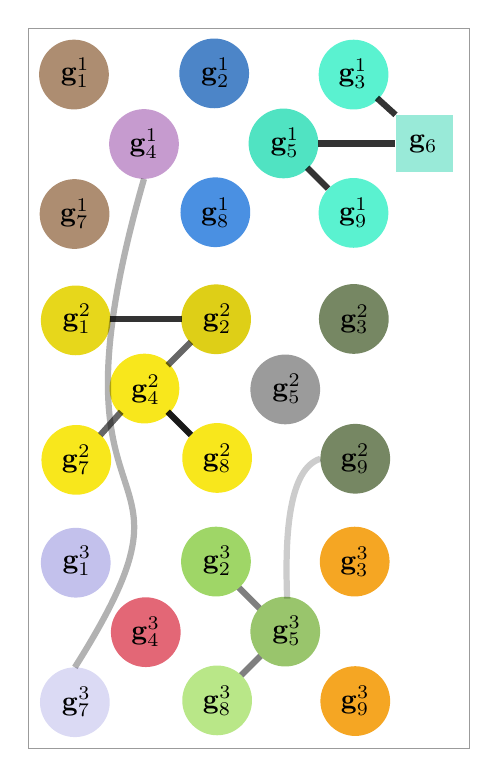
\begin{tikzpicture}[x=0.75pt,y=0.75pt,yscale=-0.56,xscale=0.56]
%uncomment if require: \path (0,1438); %set diagram left start at 0, and has height of 1438

%Shape: Rectangle [id:dp5381136388503212]
\draw  [color={rgb, 255:red, 155; green, 155; blue, 155 }  ,draw opacity=1 ] (20,700) -- (20,80) -- (400,80) -- (400,700) -- cycle ;

%Shape: Rectangle [id:dp39137146349868646]
%\draw  [color={rgb, 255:red, 155; green, 155; blue, 155 }  ,draw opacity=1 ] (21.53,491.52) -- (20.73,291.53) -- (400.72,290) -- (401.53,490) -- cycle ;

%Shape: Rectangle [id:dp3461506815581068]
%\draw  [color={rgb, 255:red, 155; green, 155; blue, 155 }  ,draw opacity=1 ] (21.53,700) -- (20.73,500) -- (400.72,498.48) -- (401.53,698.47) -- cycle ;


%Shape: Circle [id:dp12286992130015428]
\draw  [draw opacity=0][fill={rgb, 255:red, 173; green, 141; blue, 113 }  ,fill opacity=1 ] (29.84,239.84) .. controls (29.84,223.27) and (43.27,209.84) .. (59.84,209.84) .. controls (76.41,209.84) and (89.84,223.27) .. (89.84,239.84) .. controls (89.84,256.41) and (76.41,269.84) .. (59.84,269.84) .. controls (43.27,269.84) and (29.84,256.41) .. (29.84,239.84) -- cycle ;
%Shape: Circle [id:dp7931751449222735]
\draw  [draw opacity=0][fill={rgb, 255:red, 173; green, 141; blue, 113 }  ,fill opacity=1 ] (29.36,119.84) .. controls (29.36,103.27) and (42.79,89.84) .. (59.36,89.84) .. controls (75.93,89.84) and (89.36,103.27) .. (89.36,119.84) .. controls (89.36,136.41) and (75.93,149.84) .. (59.36,149.84) .. controls (42.79,149.84) and (29.36,136.41) .. (29.36,119.84) -- cycle ;
%Shape: Circle [id:dp16673433726568354]
\draw  [draw opacity=0][fill={rgb, 255:red, 170; green, 106; blue, 183 }  ,fill opacity=0.67 ] (89.6,179.6) .. controls (89.6,163.03) and (103.03,149.6) .. (119.6,149.6) .. controls (136.17,149.6) and (149.6,163.03) .. (149.6,179.6) .. controls (149.6,196.17) and (136.17,209.6) .. (119.6,209.6) .. controls (103.03,209.6) and (89.6,196.17) .. (89.6,179.6) -- cycle ;
%Shape: Circle [id:dp15511724636448365]
\draw  [draw opacity=0][fill={rgb, 255:red, 74; green, 144; blue, 226 }  ,fill opacity=1 ] (151,238.31) .. controls (151,221.74) and (164.43,208.31) .. (181,208.31) .. controls (197.57,208.31) and (211,221.74) .. (211,238.31) .. controls (211,254.88) and (197.57,268.31) .. (181,268.31) .. controls (164.43,268.31) and (151,254.88) .. (151,238.31) -- cycle ;
%Shape: Circle [id:dp8495812213022542]
\draw  [draw opacity=0][fill={rgb, 255:red, 76; green, 133; blue, 200 }  ,fill opacity=1 ] (150,118.85) .. controls (150,102.28) and (163.44,88.85) .. (180,88.85) .. controls (196.57,88.85) and (210,102.28) .. (210,118.85) .. controls (210,135.42) and (196.57,148.85) .. (180,148.85) .. controls (163.44,148.85) and (150,135.42) .. (150,118.85) -- cycle ;
%Shape: Circle [id:dp46577960716750777]
\draw  [draw opacity=0][fill={rgb, 255:red, 80; green, 227; blue, 194 }  ,fill opacity=1 ] (209.6,179.12) .. controls (209.6,162.55) and (223.03,149.12) .. (239.6,149.12) .. controls (256.17,149.12) and (269.6,162.55) .. (269.6,179.12) .. controls (269.6,195.69) and (256.17,209.12) .. (239.6,209.12) .. controls (223.03,209.12) and (209.6,195.69) .. (209.6,179.12) -- cycle ;
%Shape: Circle [id:dp30991147509029027]
\draw  [draw opacity=0][fill={rgb, 255:red, 90; green, 242; blue, 208 }  ,fill opacity=1 ] (269.84,238.88) .. controls (269.84,222.31) and (283.27,208.88) .. (299.84,208.88) .. controls (316.41,208.88) and (329.84,222.31) .. (329.84,238.88) .. controls (329.84,255.44) and (316.41,268.88) .. (299.84,268.88) .. controls (283.27,268.88) and (269.84,255.44) .. (269.84,238.88) -- cycle ;
%Shape: Circle [id:dp10962416440320566]
\draw  [draw opacity=0][fill={rgb, 255:red, 90; green, 242; blue, 208 }  ,fill opacity=1 ] (269.88,119.88) .. controls (269.88,103.31) and (283.31,89.88) .. (299.88,89.88) .. controls (316.45,89.88) and (329.88,103.31) .. (329.88,119.88) .. controls (329.88,136.45) and (316.45,149.88) .. (299.88,149.88) .. controls (283.31,149.88) and (269.88,136.45) .. (269.88,119.88) -- cycle ;

%Shape: Circle [id:dp13607314793635106]
\draw  [draw opacity=0][fill={rgb, 255:red, 248; green, 231; blue, 28 }  ,fill opacity=1 ] (31.37,451.36) .. controls (31.37,434.8) and (44.8,421.36) .. (61.37,421.36) .. controls (77.94,421.36) and (91.37,434.8) .. (91.37,451.36) .. controls (91.37,467.93) and (77.94,481.36) .. (61.37,481.36) .. controls (44.8,481.36) and (31.37,467.93) .. (31.37,451.36) -- cycle ;
%Shape: Circle [id:dp22834187586321186]
\draw  [draw opacity=0][fill={rgb, 255:red, 231; green, 215; blue, 27 }  ,fill opacity=1 ] (30.89,331.36) .. controls (30.89,314.8) and (44.32,301.36) .. (60.89,301.36) .. controls (77.46,301.36) and (90.89,314.8) .. (90.89,331.36) .. controls (90.89,347.93) and (77.46,361.36) .. (60.89,361.36) .. controls (44.32,361.36) and (30.89,347.93) .. (30.89,331.36) -- cycle ;
%Shape: Circle [id:dp9030431506925378]
\draw  [draw opacity=0][fill={rgb, 255:red, 248; green, 231; blue, 28 }  ,fill opacity=1 ] (90,390) .. controls (90,373.43) and (103.43,360) .. (120,360) .. controls (136.57,360) and (150,373.43) .. (150,390) .. controls (150,406.57) and (136.57,420) .. (120,420) .. controls (103.43,420) and (90,406.57) .. (90,390) -- cycle ;
%Shape: Circle [id:dp5036111314358263]
\draw  [draw opacity=0][fill={rgb, 255:red, 248; green, 231; blue, 28 }  ,fill opacity=1 ] (152.52,449.71) .. controls (152.52,433.15) and (165.96,419.71) .. (182.52,419.71) .. controls (199.09,419.71) and (212.52,433.15) .. (212.52,449.71) .. controls (212.52,466.28) and (199.09,479.71) .. (182.52,479.71) .. controls (165.96,479.71) and (152.52,466.28) .. (152.52,449.71) -- cycle ;
%Shape: Circle [id:dp28094865389913615]
\draw  [draw opacity=0][fill={rgb, 255:red, 222; green, 207; blue, 23 }  ,fill opacity=1 ] (151.65,330.38) .. controls (151.65,313.81) and (165.08,300.38) .. (181.65,300.38) .. controls (198.22,300.38) and (211.65,313.81) .. (211.65,330.38) .. controls (211.65,346.94) and (198.22,360.38) .. (181.65,360.38) .. controls (165.08,360.38) and (151.65,346.94) .. (151.65,330.38) -- cycle ;
%Shape: Circle [id:dp8199553596351965]
\draw  [draw opacity=0][fill={rgb, 255:red, 155; green, 155; blue, 155 }  ,fill opacity=1 ] (211.13,390.76) .. controls (211.13,374.19) and (224.56,360.76) .. (241.13,360.76) .. controls (257.7,360.76) and (271.13,374.19) .. (271.13,390.76) .. controls (271.13,407.33) and (257.7,420.76) .. (241.13,420.76) .. controls (224.56,420.76) and (211.13,407.33) .. (211.13,390.76) -- cycle ;
%Shape: Circle [id:dp061627101972308695]
\draw  [draw opacity=0][fill={rgb, 255:red, 34; green, 61; blue, 3 }  ,fill opacity=0.62 ] (271.37,450.4) .. controls (271.37,433.83) and (284.8,420.4) .. (301.37,420.4) .. controls (317.94,420.4) and (331.37,433.83) .. (331.37,450.4) .. controls (331.37,466.97) and (317.94,480.4) .. (301.37,480.4) .. controls (284.8,480.4) and (271.37,466.97) .. (271.37,450.4) -- cycle ;
%Shape: Circle [id:dp6586711959399798]
\draw  [draw opacity=0][fill={rgb, 255:red, 34; green, 61; blue, 3 }  ,fill opacity=0.62 ] (270.12,330.12) .. controls (270.12,313.55) and (283.55,300.12) .. (300.12,300.12) .. controls (316.69,300.12) and (330.12,313.55) .. (330.12,330.12) .. controls (330.12,346.69) and (316.69,360.12) .. (300.12,360.12) .. controls (283.55,360.12) and (270.12,346.69) .. (270.12,330.12) -- cycle ;
%Straight Lines [id:da09795376579003179]
\draw [color={rgb, 255:red, 0; green, 0; blue, 0 }  ,draw opacity=0.5 ][line width=2.25]    (200,640) -- (220,620) ;
%Straight Lines [id:da13253659772522353]
\draw [color={rgb, 255:red, 0; green, 0; blue, 0 }  ,draw opacity=0.5 ][line width=2.25]    (200,560) -- (220,580) ;

%Shape: Circle [id:dp07594340015479584]
\draw  [draw opacity=0][fill={rgb, 255:red, 195; green, 193; blue, 236 }  ,fill opacity=0.6 ] (30.12,659.88) .. controls (30.12,643.31) and (43.55,629.88) .. (60.12,629.88) .. controls (76.69,629.88) and (90.12,643.31) .. (90.12,659.88) .. controls (90.12,676.45) and (76.69,689.88) .. (60.12,689.88) .. controls (43.55,689.88) and (30.12,676.45) .. (30.12,659.88) -- cycle ;
%Shape: Circle [id:dp6610712869287463]
\draw  [draw opacity=0][fill={rgb, 255:red, 195; green, 193; blue, 236 }  ,fill opacity=1 ] (30.89,539.84) .. controls (30.89,523.27) and (44.32,509.84) .. (60.89,509.84) .. controls (77.46,509.84) and (90.89,523.27) .. (90.89,539.84) .. controls (90.89,556.41) and (77.46,569.84) .. (60.89,569.84) .. controls (44.32,569.84) and (30.89,556.41) .. (30.89,539.84) -- cycle ;
%Shape: Circle [id:dp7622423737356947]
\draw  [draw opacity=0][fill={rgb, 255:red, 208; green, 2; blue, 27 }  ,fill opacity=0.6 ] (121.25,629.6) .. controls (104.68,629.67) and (91.19,616.29) .. (91.13,599.72) .. controls (91.06,583.15) and (104.44,569.67) .. (121.01,569.6) .. controls (137.58,569.53) and (151.06,582.91) .. (151.13,599.48) .. controls (151.19,616.05) and (137.82,629.53) .. (121.25,629.6) -- cycle ;
%Shape: Circle [id:dp4084876787586895]
\draw  [draw opacity=0][fill={rgb, 255:red, 185; green, 231; blue, 136 }  ,fill opacity=1 ] (152.52,658.31) .. controls (152.52,641.74) and (165.96,628.31) .. (182.52,628.31) .. controls (199.09,628.31) and (212.52,641.74) .. (212.52,658.31) .. controls (212.52,674.88) and (199.09,688.31) .. (182.52,688.31) .. controls (165.96,688.31) and (152.52,674.88) .. (152.52,658.31) -- cycle ;
%Shape: Circle [id:dp5875693847671164]
\draw  [draw opacity=0][fill={rgb, 255:red, 159; green, 214; blue, 103 }  ,fill opacity=1 ] (151.53,538.85) .. controls (151.53,522.28) and (164.96,508.85) .. (181.53,508.85) .. controls (198.1,508.85) and (211.53,522.28) .. (211.53,538.85) .. controls (211.53,555.42) and (198.1,568.85) .. (181.53,568.85) .. controls (164.96,568.85) and (151.53,555.42) .. (151.53,538.85) -- cycle ;
%Shape: Circle [id:dp06003724860547344]
\draw  [draw opacity=0][fill={rgb, 255:red, 153; green, 197; blue, 108 }  ,fill opacity=1 ] (211.13,599.12) .. controls (211.13,582.55) and (224.56,569.12) .. (241.13,569.12) .. controls (257.7,569.12) and (271.13,582.55) .. (271.13,599.12) .. controls (271.13,615.69) and (257.7,629.12) .. (241.13,629.12) .. controls (224.56,629.12) and (211.13,615.69) .. (211.13,599.12) -- cycle ;
%Shape: Circle [id:dp3947958928282629]
\draw  [draw opacity=0][fill={rgb, 255:red, 245; green, 166; blue, 35 }  ,fill opacity=1 ] (271.37,658.88) .. controls (271.37,642.31) and (284.8,628.88) .. (301.37,628.88) .. controls (317.94,628.88) and (331.37,642.31) .. (331.37,658.88) .. controls (331.37,675.44) and (317.94,688.88) .. (301.37,688.88) .. controls (284.8,688.88) and (271.37,675.44) .. (271.37,658.88) -- cycle ;
%Shape: Circle [id:dp18102804016986096]
\draw  [draw opacity=0][fill={rgb, 255:red, 245; green, 166; blue, 35 }  ,fill
opacity=1 ] (270.89,538.88) .. controls (270.89,522.31) and (284.32,508.88)
.. (300.89,508.88) .. controls (317.45,508.88) and (330.89,522.31)
.. (330.89,538.88) .. controls (330.89,555.45) and (317.45,568.88)
.. (300.89,568.88) .. controls (284.32,568.88) and (270.89,555.45)
.. (270.89,538.88) -- cycle ;
%Curve Lines [id:da3377087525660538] 
\draw [color={rgb, 255:red, 0; green, 0; blue, 0 }  ,draw opacity=0.3 ][line width=2.25]    (119.6,209.6) .. controls (25.8,536) and (186.8,429) .. (60.12,629.88) ;
%Straight Lines [id:da43642919945499603]
\draw [color={rgb, 255:red, 0; green, 0; blue, 0 }  ,draw opacity=0.8 ][line width=2.25]    (90,330) -- (152,330) ; %remember!
%Straight Lines [id:da8359064659577915]
\draw [color={rgb, 255:red, 0; green, 0; blue, 0 }  ,draw opacity=0.6 ][line width=2.25]    (140,370) -- (160,350) ;
%Straight Lines [id:da367274331259694]
\draw [color={rgb, 255:red, 0; green, 0; blue, 0 }  ,draw opacity=0.6 ][line width=2.25]    (82,430) -- (100,410) ;
%Straight Lines [id:da7756630094250268]
\draw [color={rgb, 255:red, 0; green, 0; blue, 0 }  ,draw opacity=0.9 ][line width=2.25]    (140,410) -- (160,430) ;
%Straight Lines [id:da31290273671454116]
\draw [color={rgb, 255:red, 0; green, 0; blue, 0 }  ,draw opacity=0.8 ][line width=2.25]    (260,200) -- (278,218) ;
%Straight Lines [id:da8522668149365773]
\draw [color={rgb, 255:red, 0; green, 0; blue, 0 }  ,draw opacity=0.8 ][line width=2.25]    (336,154.5) -- (320,140) ;
%Straight Lines [id:da771798416536507]
\draw [color={rgb, 255:red, 0; green, 0; blue, 0 }  ,draw opacity=0.8 ][line width=2.25]    (269.6,179.12) -- (335.6,179.12) ;
%Curve Lines [id:da8781500202610568]
\draw [color={rgb, 255:red, 0; green, 0; blue, 0 }  ,draw opacity=0.2 ][line width=2.25]    (242.77,570.74) .. controls (240.51,513.97) and (244.58,458.67) .. (271.37,450.4) ;
%Shape: Square [id:dp2620517183205848]
\draw  [draw opacity=0][fill={rgb, 255:red, 153; green, 234; blue, 216 }  ,fill opacity=1 ] (336,154.5) -- (385.5,154.5) -- (385.5,204) -- (336,204) -- cycle ;

% Text Node
\draw (299.36,118.88) node   [align=left] {$\vec g_{3}^1$};
% Text Node
\draw (59.84,239.84) node   [align=left] {$\vec g_{7}^1$};
% Text Node
\draw (240.89,178.54) node   [align=left] {$\vec g_{5}^1$};
% Text Node
\draw (181.19,238.46) node   [align=left] {$\vec g_{8}^1$};
% Text Node
\draw (119.6,179.6) node   [align=left] {$\vec g_{4}^1$};
% Text Node
\draw (181.17,118.51) node   [align=left] {$\vec g_{2}^1$};
% Text Node
\draw (60.36,118.42) node   [align=left] {$\vec g_{1}^1$};
% Text Node
\draw (299.84,238.88) node   [align=left] {$\vec g_{9}^1$};

% Text Node
\draw (300.89,330.4) node   [align=left] {$\vec g_{3}^2$};
% Text Node
\draw (61.37,451.36) node   [align=left] {$\vec g_{7}^2$};
% Text Node
\draw (242.41,390.07) node   [align=left] {$\vec g_{5}^2$};
% Text Node
\draw (182.72,449.98) node   [align=left] {$\vec g_{8}^2$};
% Text Node
\draw (121.13,391.12) node   [align=left] {$\vec g_{4}^2$};
% Text Node
\draw (182.69,330.04) node   [align=left] {$\vec g_{2}^2$};
% Text Node
\draw (61.89,329.94) node  [align=left] {$\vec g_{1}^2$};
% Text Node
\draw (301.37,450.4) node   [align=left] {$\vec g_{9}^2$};

% Text Node
\draw (300.89,538.88) node   [align=left] {$\vec g_{3}^3$};
% Text Node
\draw (61.37,659.84) node   [align=left] {$\vec g_{7}^3$};
% Text Node
\draw (242.41,598.54) node   [align=left] {$\vec g_{5}^3$};
% Text Node
\draw (182.72,658.46) node   [align=left] {$\vec g_{8}^3$};
% Text Node
\draw (121.13,599.6) node   [align=left] {$\vec g_{4}^3$};
% Text Node
\draw (182.69,538.51) node   [align=left] {$\vec g_{2}^3$};
% Text Node
\draw (61.89,538.42) node [align=left] {$\vec g_{1}^3$};
% Text Node
\draw (301.37,658.88) node   [align=left] {$\vec g_{9}^3$};

% Text Node
\draw (360,180) node   [align=left] {$\vec g_{6}$};


\end{tikzpicture}

    \end{column}
  \end{columns}
  
\end{frame}



% \begin{frame}
%   \frametitle{Clustering of the Variant Graph}


%   \vspace{-0.5cm}
%   \begin{columns}[T,onlytextwidth]
%     \begin{column}{0.6\textwidth}
  
%       \begin{itemize}
%       \item requires an adapted Marcovian clustering
%       \item considers higher order neighbors
%       \item yields consistent clusters
%       \item directly yields the parent orientation              
%       \item is as fast as the graph based approach
%       \item provides probabilities for all parent variants
%       \item allows to include morphological features
%       \end{itemize}
           
%     \end{column}
%     \begin{column}{0.38\textwidth}

%       \vspace{-1cm}
%       \begin{overlayarea}{\textwidth}{\textheight}
%         \begin{onlyenv}<1>
%           \tikzset{every picture/.style={line width=0.75pt}} %set default line width to 0.75pt

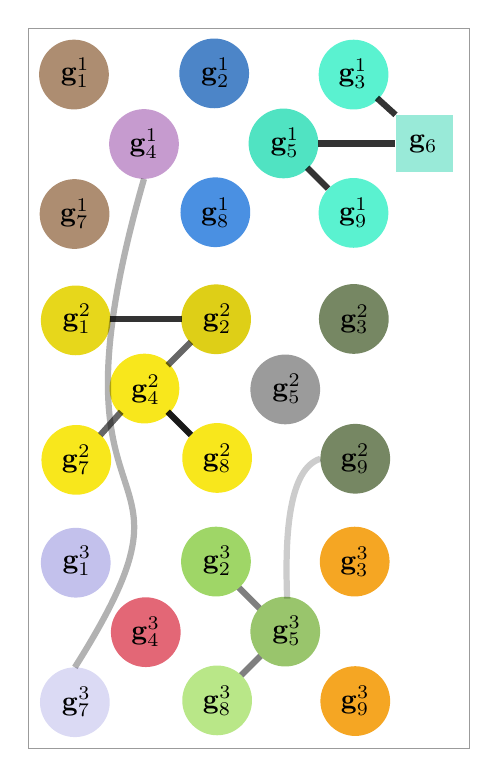
\begin{tikzpicture}[x=0.75pt,y=0.75pt,yscale=-0.56,xscale=0.56]
%uncomment if require: \path (0,1438); %set diagram left start at 0, and has height of 1438

%Shape: Rectangle [id:dp5381136388503212]
\draw  [color={rgb, 255:red, 155; green, 155; blue, 155 }  ,draw opacity=1 ] (20,700) -- (20,80) -- (400,80) -- (400,700) -- cycle ;

%Shape: Rectangle [id:dp39137146349868646]
%\draw  [color={rgb, 255:red, 155; green, 155; blue, 155 }  ,draw opacity=1 ] (21.53,491.52) -- (20.73,291.53) -- (400.72,290) -- (401.53,490) -- cycle ;

%Shape: Rectangle [id:dp3461506815581068]
%\draw  [color={rgb, 255:red, 155; green, 155; blue, 155 }  ,draw opacity=1 ] (21.53,700) -- (20.73,500) -- (400.72,498.48) -- (401.53,698.47) -- cycle ;


%Shape: Circle [id:dp12286992130015428]
\draw  [draw opacity=0][fill={rgb, 255:red, 173; green, 141; blue, 113 }  ,fill opacity=1 ] (29.84,239.84) .. controls (29.84,223.27) and (43.27,209.84) .. (59.84,209.84) .. controls (76.41,209.84) and (89.84,223.27) .. (89.84,239.84) .. controls (89.84,256.41) and (76.41,269.84) .. (59.84,269.84) .. controls (43.27,269.84) and (29.84,256.41) .. (29.84,239.84) -- cycle ;
%Shape: Circle [id:dp7931751449222735]
\draw  [draw opacity=0][fill={rgb, 255:red, 173; green, 141; blue, 113 }  ,fill opacity=1 ] (29.36,119.84) .. controls (29.36,103.27) and (42.79,89.84) .. (59.36,89.84) .. controls (75.93,89.84) and (89.36,103.27) .. (89.36,119.84) .. controls (89.36,136.41) and (75.93,149.84) .. (59.36,149.84) .. controls (42.79,149.84) and (29.36,136.41) .. (29.36,119.84) -- cycle ;
%Shape: Circle [id:dp16673433726568354]
\draw  [draw opacity=0][fill={rgb, 255:red, 170; green, 106; blue, 183 }  ,fill opacity=0.67 ] (89.6,179.6) .. controls (89.6,163.03) and (103.03,149.6) .. (119.6,149.6) .. controls (136.17,149.6) and (149.6,163.03) .. (149.6,179.6) .. controls (149.6,196.17) and (136.17,209.6) .. (119.6,209.6) .. controls (103.03,209.6) and (89.6,196.17) .. (89.6,179.6) -- cycle ;
%Shape: Circle [id:dp15511724636448365]
\draw  [draw opacity=0][fill={rgb, 255:red, 74; green, 144; blue, 226 }  ,fill opacity=1 ] (151,238.31) .. controls (151,221.74) and (164.43,208.31) .. (181,208.31) .. controls (197.57,208.31) and (211,221.74) .. (211,238.31) .. controls (211,254.88) and (197.57,268.31) .. (181,268.31) .. controls (164.43,268.31) and (151,254.88) .. (151,238.31) -- cycle ;
%Shape: Circle [id:dp8495812213022542]
\draw  [draw opacity=0][fill={rgb, 255:red, 76; green, 133; blue, 200 }  ,fill opacity=1 ] (150,118.85) .. controls (150,102.28) and (163.44,88.85) .. (180,88.85) .. controls (196.57,88.85) and (210,102.28) .. (210,118.85) .. controls (210,135.42) and (196.57,148.85) .. (180,148.85) .. controls (163.44,148.85) and (150,135.42) .. (150,118.85) -- cycle ;
%Shape: Circle [id:dp46577960716750777]
\draw  [draw opacity=0][fill={rgb, 255:red, 80; green, 227; blue, 194 }  ,fill opacity=1 ] (209.6,179.12) .. controls (209.6,162.55) and (223.03,149.12) .. (239.6,149.12) .. controls (256.17,149.12) and (269.6,162.55) .. (269.6,179.12) .. controls (269.6,195.69) and (256.17,209.12) .. (239.6,209.12) .. controls (223.03,209.12) and (209.6,195.69) .. (209.6,179.12) -- cycle ;
%Shape: Circle [id:dp30991147509029027]
\draw  [draw opacity=0][fill={rgb, 255:red, 90; green, 242; blue, 208 }  ,fill opacity=1 ] (269.84,238.88) .. controls (269.84,222.31) and (283.27,208.88) .. (299.84,208.88) .. controls (316.41,208.88) and (329.84,222.31) .. (329.84,238.88) .. controls (329.84,255.44) and (316.41,268.88) .. (299.84,268.88) .. controls (283.27,268.88) and (269.84,255.44) .. (269.84,238.88) -- cycle ;
%Shape: Circle [id:dp10962416440320566]
\draw  [draw opacity=0][fill={rgb, 255:red, 90; green, 242; blue, 208 }  ,fill opacity=1 ] (269.88,119.88) .. controls (269.88,103.31) and (283.31,89.88) .. (299.88,89.88) .. controls (316.45,89.88) and (329.88,103.31) .. (329.88,119.88) .. controls (329.88,136.45) and (316.45,149.88) .. (299.88,149.88) .. controls (283.31,149.88) and (269.88,136.45) .. (269.88,119.88) -- cycle ;

%Shape: Circle [id:dp13607314793635106]
\draw  [draw opacity=0][fill={rgb, 255:red, 248; green, 231; blue, 28 }  ,fill opacity=1 ] (31.37,451.36) .. controls (31.37,434.8) and (44.8,421.36) .. (61.37,421.36) .. controls (77.94,421.36) and (91.37,434.8) .. (91.37,451.36) .. controls (91.37,467.93) and (77.94,481.36) .. (61.37,481.36) .. controls (44.8,481.36) and (31.37,467.93) .. (31.37,451.36) -- cycle ;
%Shape: Circle [id:dp22834187586321186]
\draw  [draw opacity=0][fill={rgb, 255:red, 231; green, 215; blue, 27 }  ,fill opacity=1 ] (30.89,331.36) .. controls (30.89,314.8) and (44.32,301.36) .. (60.89,301.36) .. controls (77.46,301.36) and (90.89,314.8) .. (90.89,331.36) .. controls (90.89,347.93) and (77.46,361.36) .. (60.89,361.36) .. controls (44.32,361.36) and (30.89,347.93) .. (30.89,331.36) -- cycle ;
%Shape: Circle [id:dp9030431506925378]
\draw  [draw opacity=0][fill={rgb, 255:red, 248; green, 231; blue, 28 }  ,fill opacity=1 ] (90,390) .. controls (90,373.43) and (103.43,360) .. (120,360) .. controls (136.57,360) and (150,373.43) .. (150,390) .. controls (150,406.57) and (136.57,420) .. (120,420) .. controls (103.43,420) and (90,406.57) .. (90,390) -- cycle ;
%Shape: Circle [id:dp5036111314358263]
\draw  [draw opacity=0][fill={rgb, 255:red, 248; green, 231; blue, 28 }  ,fill opacity=1 ] (152.52,449.71) .. controls (152.52,433.15) and (165.96,419.71) .. (182.52,419.71) .. controls (199.09,419.71) and (212.52,433.15) .. (212.52,449.71) .. controls (212.52,466.28) and (199.09,479.71) .. (182.52,479.71) .. controls (165.96,479.71) and (152.52,466.28) .. (152.52,449.71) -- cycle ;
%Shape: Circle [id:dp28094865389913615]
\draw  [draw opacity=0][fill={rgb, 255:red, 222; green, 207; blue, 23 }  ,fill opacity=1 ] (151.65,330.38) .. controls (151.65,313.81) and (165.08,300.38) .. (181.65,300.38) .. controls (198.22,300.38) and (211.65,313.81) .. (211.65,330.38) .. controls (211.65,346.94) and (198.22,360.38) .. (181.65,360.38) .. controls (165.08,360.38) and (151.65,346.94) .. (151.65,330.38) -- cycle ;
%Shape: Circle [id:dp8199553596351965]
\draw  [draw opacity=0][fill={rgb, 255:red, 155; green, 155; blue, 155 }  ,fill opacity=1 ] (211.13,390.76) .. controls (211.13,374.19) and (224.56,360.76) .. (241.13,360.76) .. controls (257.7,360.76) and (271.13,374.19) .. (271.13,390.76) .. controls (271.13,407.33) and (257.7,420.76) .. (241.13,420.76) .. controls (224.56,420.76) and (211.13,407.33) .. (211.13,390.76) -- cycle ;
%Shape: Circle [id:dp061627101972308695]
\draw  [draw opacity=0][fill={rgb, 255:red, 34; green, 61; blue, 3 }  ,fill opacity=0.62 ] (271.37,450.4) .. controls (271.37,433.83) and (284.8,420.4) .. (301.37,420.4) .. controls (317.94,420.4) and (331.37,433.83) .. (331.37,450.4) .. controls (331.37,466.97) and (317.94,480.4) .. (301.37,480.4) .. controls (284.8,480.4) and (271.37,466.97) .. (271.37,450.4) -- cycle ;
%Shape: Circle [id:dp6586711959399798]
\draw  [draw opacity=0][fill={rgb, 255:red, 34; green, 61; blue, 3 }  ,fill opacity=0.62 ] (270.12,330.12) .. controls (270.12,313.55) and (283.55,300.12) .. (300.12,300.12) .. controls (316.69,300.12) and (330.12,313.55) .. (330.12,330.12) .. controls (330.12,346.69) and (316.69,360.12) .. (300.12,360.12) .. controls (283.55,360.12) and (270.12,346.69) .. (270.12,330.12) -- cycle ;
%Straight Lines [id:da09795376579003179]
\draw [color={rgb, 255:red, 0; green, 0; blue, 0 }  ,draw opacity=0.5 ][line width=2.25]    (200,640) -- (220,620) ;
%Straight Lines [id:da13253659772522353]
\draw [color={rgb, 255:red, 0; green, 0; blue, 0 }  ,draw opacity=0.5 ][line width=2.25]    (200,560) -- (220,580) ;

%Shape: Circle [id:dp07594340015479584]
\draw  [draw opacity=0][fill={rgb, 255:red, 195; green, 193; blue, 236 }  ,fill opacity=0.6 ] (30.12,659.88) .. controls (30.12,643.31) and (43.55,629.88) .. (60.12,629.88) .. controls (76.69,629.88) and (90.12,643.31) .. (90.12,659.88) .. controls (90.12,676.45) and (76.69,689.88) .. (60.12,689.88) .. controls (43.55,689.88) and (30.12,676.45) .. (30.12,659.88) -- cycle ;
%Shape: Circle [id:dp6610712869287463]
\draw  [draw opacity=0][fill={rgb, 255:red, 195; green, 193; blue, 236 }  ,fill opacity=1 ] (30.89,539.84) .. controls (30.89,523.27) and (44.32,509.84) .. (60.89,509.84) .. controls (77.46,509.84) and (90.89,523.27) .. (90.89,539.84) .. controls (90.89,556.41) and (77.46,569.84) .. (60.89,569.84) .. controls (44.32,569.84) and (30.89,556.41) .. (30.89,539.84) -- cycle ;
%Shape: Circle [id:dp7622423737356947]
\draw  [draw opacity=0][fill={rgb, 255:red, 208; green, 2; blue, 27 }  ,fill opacity=0.6 ] (121.25,629.6) .. controls (104.68,629.67) and (91.19,616.29) .. (91.13,599.72) .. controls (91.06,583.15) and (104.44,569.67) .. (121.01,569.6) .. controls (137.58,569.53) and (151.06,582.91) .. (151.13,599.48) .. controls (151.19,616.05) and (137.82,629.53) .. (121.25,629.6) -- cycle ;
%Shape: Circle [id:dp4084876787586895]
\draw  [draw opacity=0][fill={rgb, 255:red, 185; green, 231; blue, 136 }  ,fill opacity=1 ] (152.52,658.31) .. controls (152.52,641.74) and (165.96,628.31) .. (182.52,628.31) .. controls (199.09,628.31) and (212.52,641.74) .. (212.52,658.31) .. controls (212.52,674.88) and (199.09,688.31) .. (182.52,688.31) .. controls (165.96,688.31) and (152.52,674.88) .. (152.52,658.31) -- cycle ;
%Shape: Circle [id:dp5875693847671164]
\draw  [draw opacity=0][fill={rgb, 255:red, 159; green, 214; blue, 103 }  ,fill opacity=1 ] (151.53,538.85) .. controls (151.53,522.28) and (164.96,508.85) .. (181.53,508.85) .. controls (198.1,508.85) and (211.53,522.28) .. (211.53,538.85) .. controls (211.53,555.42) and (198.1,568.85) .. (181.53,568.85) .. controls (164.96,568.85) and (151.53,555.42) .. (151.53,538.85) -- cycle ;
%Shape: Circle [id:dp06003724860547344]
\draw  [draw opacity=0][fill={rgb, 255:red, 153; green, 197; blue, 108 }  ,fill opacity=1 ] (211.13,599.12) .. controls (211.13,582.55) and (224.56,569.12) .. (241.13,569.12) .. controls (257.7,569.12) and (271.13,582.55) .. (271.13,599.12) .. controls (271.13,615.69) and (257.7,629.12) .. (241.13,629.12) .. controls (224.56,629.12) and (211.13,615.69) .. (211.13,599.12) -- cycle ;
%Shape: Circle [id:dp3947958928282629]
\draw  [draw opacity=0][fill={rgb, 255:red, 245; green, 166; blue, 35 }  ,fill opacity=1 ] (271.37,658.88) .. controls (271.37,642.31) and (284.8,628.88) .. (301.37,628.88) .. controls (317.94,628.88) and (331.37,642.31) .. (331.37,658.88) .. controls (331.37,675.44) and (317.94,688.88) .. (301.37,688.88) .. controls (284.8,688.88) and (271.37,675.44) .. (271.37,658.88) -- cycle ;
%Shape: Circle [id:dp18102804016986096]
\draw  [draw opacity=0][fill={rgb, 255:red, 245; green, 166; blue, 35 }  ,fill
opacity=1 ] (270.89,538.88) .. controls (270.89,522.31) and (284.32,508.88)
.. (300.89,508.88) .. controls (317.45,508.88) and (330.89,522.31)
.. (330.89,538.88) .. controls (330.89,555.45) and (317.45,568.88)
.. (300.89,568.88) .. controls (284.32,568.88) and (270.89,555.45)
.. (270.89,538.88) -- cycle ;
%Curve Lines [id:da3377087525660538] 
\draw [color={rgb, 255:red, 0; green, 0; blue, 0 }  ,draw opacity=0.3 ][line width=2.25]    (119.6,209.6) .. controls (25.8,536) and (186.8,429) .. (60.12,629.88) ;
%Straight Lines [id:da43642919945499603]
\draw [color={rgb, 255:red, 0; green, 0; blue, 0 }  ,draw opacity=0.8 ][line width=2.25]    (90,330) -- (152,330) ; %remember!
%Straight Lines [id:da8359064659577915]
\draw [color={rgb, 255:red, 0; green, 0; blue, 0 }  ,draw opacity=0.6 ][line width=2.25]    (140,370) -- (160,350) ;
%Straight Lines [id:da367274331259694]
\draw [color={rgb, 255:red, 0; green, 0; blue, 0 }  ,draw opacity=0.6 ][line width=2.25]    (82,430) -- (100,410) ;
%Straight Lines [id:da7756630094250268]
\draw [color={rgb, 255:red, 0; green, 0; blue, 0 }  ,draw opacity=0.9 ][line width=2.25]    (140,410) -- (160,430) ;
%Straight Lines [id:da31290273671454116]
\draw [color={rgb, 255:red, 0; green, 0; blue, 0 }  ,draw opacity=0.8 ][line width=2.25]    (260,200) -- (278,218) ;
%Straight Lines [id:da8522668149365773]
\draw [color={rgb, 255:red, 0; green, 0; blue, 0 }  ,draw opacity=0.8 ][line width=2.25]    (336,154.5) -- (320,140) ;
%Straight Lines [id:da771798416536507]
\draw [color={rgb, 255:red, 0; green, 0; blue, 0 }  ,draw opacity=0.8 ][line width=2.25]    (269.6,179.12) -- (335.6,179.12) ;
%Curve Lines [id:da8781500202610568]
\draw [color={rgb, 255:red, 0; green, 0; blue, 0 }  ,draw opacity=0.2 ][line width=2.25]    (242.77,570.74) .. controls (240.51,513.97) and (244.58,458.67) .. (271.37,450.4) ;
%Shape: Square [id:dp2620517183205848]
\draw  [draw opacity=0][fill={rgb, 255:red, 153; green, 234; blue, 216 }  ,fill opacity=1 ] (336,154.5) -- (385.5,154.5) -- (385.5,204) -- (336,204) -- cycle ;

% Text Node
\draw (299.36,118.88) node   [align=left] {$\vec g_{3}^1$};
% Text Node
\draw (59.84,239.84) node   [align=left] {$\vec g_{7}^1$};
% Text Node
\draw (240.89,178.54) node   [align=left] {$\vec g_{5}^1$};
% Text Node
\draw (181.19,238.46) node   [align=left] {$\vec g_{8}^1$};
% Text Node
\draw (119.6,179.6) node   [align=left] {$\vec g_{4}^1$};
% Text Node
\draw (181.17,118.51) node   [align=left] {$\vec g_{2}^1$};
% Text Node
\draw (60.36,118.42) node   [align=left] {$\vec g_{1}^1$};
% Text Node
\draw (299.84,238.88) node   [align=left] {$\vec g_{9}^1$};

% Text Node
\draw (300.89,330.4) node   [align=left] {$\vec g_{3}^2$};
% Text Node
\draw (61.37,451.36) node   [align=left] {$\vec g_{7}^2$};
% Text Node
\draw (242.41,390.07) node   [align=left] {$\vec g_{5}^2$};
% Text Node
\draw (182.72,449.98) node   [align=left] {$\vec g_{8}^2$};
% Text Node
\draw (121.13,391.12) node   [align=left] {$\vec g_{4}^2$};
% Text Node
\draw (182.69,330.04) node   [align=left] {$\vec g_{2}^2$};
% Text Node
\draw (61.89,329.94) node  [align=left] {$\vec g_{1}^2$};
% Text Node
\draw (301.37,450.4) node   [align=left] {$\vec g_{9}^2$};

% Text Node
\draw (300.89,538.88) node   [align=left] {$\vec g_{3}^3$};
% Text Node
\draw (61.37,659.84) node   [align=left] {$\vec g_{7}^3$};
% Text Node
\draw (242.41,598.54) node   [align=left] {$\vec g_{5}^3$};
% Text Node
\draw (182.72,658.46) node   [align=left] {$\vec g_{8}^3$};
% Text Node
\draw (121.13,599.6) node   [align=left] {$\vec g_{4}^3$};
% Text Node
\draw (182.69,538.51) node   [align=left] {$\vec g_{2}^3$};
% Text Node
\draw (61.89,538.42) node [align=left] {$\vec g_{1}^3$};
% Text Node
\draw (301.37,658.88) node   [align=left] {$\vec g_{9}^3$};

% Text Node
\draw (360,180) node   [align=left] {$\vec g_{6}$};


\end{tikzpicture}

%         \end{onlyenv}
%                 \begin{onlyenv}<2>
%           \tikzset{every picture/.style={line width=0.75pt}} %set default line width to 0.75pt

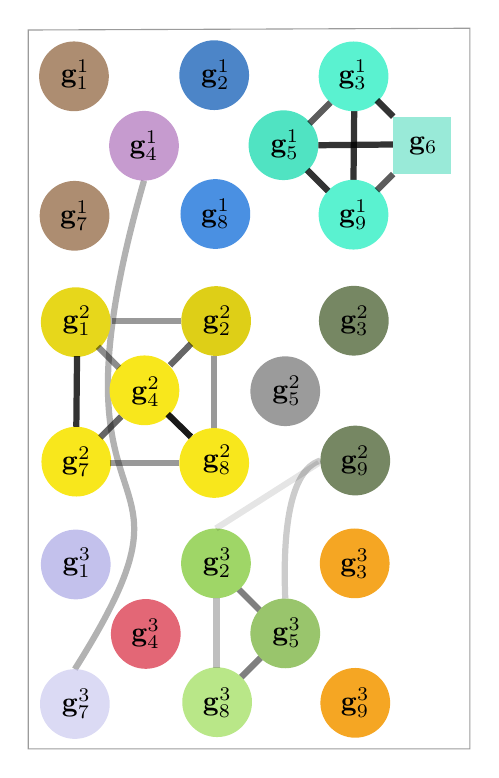
\begin{tikzpicture}[x=0.75pt,y=0.75pt,yscale=-0.56,xscale=0.56]
%uncomment if require: \path (0,1438); %set diagram left start at 0, and has height of 1438

%Shape: Rectangle [id:dp123913868933059]
\draw  [color={rgb, 255:red, 155; green, 155; blue, 155 }  ,draw opacity=1 ] (40,1426) -- (40,807.5) -- (420,805.98) -- (420,1426) -- cycle ;

%Shape: Rectangle [id:dp4611404146641136]
%\draw  [color={rgb, 255:red, 155; green, 155; blue, 155 }  ,draw opacity=1 ] (41.53,1219.02) -- (40.73,1019.03) -- (420.72,1017.5) -- (421.53,1217.5) -- cycle ;

%Shape: Rectangle [id:dp7067341610923232]
%\draw  [color={rgb, 255:red, 155; green, 155; blue, 155 }  ,draw opacity=1 ] (41.53,1427.5) -- (40.73,1227.5) -- (420.72,1225.98) -- (421.53,1425.97) -- cycle ;


%Curve Lines [id:da8765379547010526] 
\draw [color={rgb, 255:red, 0; green, 0; blue, 0 }  ,draw opacity=0.3 ][line
width=2.25]    (139.6,937.1) .. controls (45.8,1263.5) and (206.8,1156.5)
.. (80.12,1357.38) ;

%Straight Lines [id:da6136156323752866] 
\draw [color={rgb, 255:red, 0; green, 0; blue, 0 }  ,draw opacity=0.4 ][line width=2.25]    (111.65,1057.88) -- (171.65,1057.88) ;
%Straight Lines [id:da32087762157406585] 
\draw [color={rgb, 255:red, 0; green, 0; blue, 0 }  ,draw opacity=0.8 ][line width=2.25]    (319.84,936.38) -- (320.47,875.51) ;


%Shape: Circle [id:dp8315189874132158]
\draw  [draw opacity=0][fill={rgb, 255:red, 173; green, 141; blue, 113 }  ,fill opacity=1 ] (49.84,967.34) .. controls (49.84,950.77) and (63.27,937.34) .. (79.84,937.34) .. controls (96.41,937.34) and (109.84,950.77) .. (109.84,967.34) .. controls (109.84,983.91) and (96.41,997.34) .. (79.84,997.34) .. controls (63.27,997.34) and (49.84,983.91) .. (49.84,967.34) -- cycle ;
%Shape: Circle [id:dp09074519405437909]
\draw  [draw opacity=0][fill={rgb, 255:red, 173; green, 141; blue, 113 }  ,fill opacity=1 ] (49.36,847.34) .. controls (49.36,830.77) and (62.79,817.34) .. (79.36,817.34) .. controls (95.93,817.34) and (109.36,830.77) .. (109.36,847.34) .. controls (109.36,863.91) and (95.93,877.34) .. (79.36,877.34) .. controls (62.79,877.34) and (49.36,863.91) .. (49.36,847.34) -- cycle ;
%Shape: Circle [id:dp19314789147617262]
\draw  [draw opacity=0][fill={rgb, 255:red, 170; green, 106; blue, 183 }  ,fill opacity=0.67 ] (109.6,907.1) .. controls (109.6,890.53) and (123.03,877.1) .. (139.6,877.1) .. controls (156.17,877.1) and (169.6,890.53) .. (169.6,907.1) .. controls (169.6,923.67) and (156.17,937.1) .. (139.6,937.1) .. controls (123.03,937.1) and (109.6,923.67) .. (109.6,907.1) -- cycle ;
%Shape: Circle [id:dp11323621622465652]
\draw  [draw opacity=0][fill={rgb, 255:red, 74; green, 144; blue, 226 }  ,fill opacity=1 ] (171,965.81) .. controls (171,949.24) and (184.43,935.81) .. (201,935.81) .. controls (217.57,935.81) and (231,949.24) .. (231,965.81) .. controls (231,982.38) and (217.57,995.81) .. (201,995.81) .. controls (184.43,995.81) and (171,982.38) .. (171,965.81) -- cycle ;
%Shape: Circle [id:dp8714656767395375]
\draw  [draw opacity=0][fill={rgb, 255:red, 76; green, 133; blue, 200 }  ,fill opacity=1 ] (170,846.35) .. controls (170,829.78) and (183.44,816.35) .. (200,816.35) .. controls (216.57,816.35) and (230,829.78) .. (230,846.35) .. controls (230,862.92) and (216.57,876.35) .. (200,876.35) .. controls (183.44,876.35) and (170,862.92) .. (170,846.35) -- cycle ;
%Shape: Circle [id:dp43339761210898353]
\draw  [draw opacity=0][fill={rgb, 255:red, 80; green, 227; blue, 194 }  ,fill opacity=1 ] (229.6,906.62) .. controls (229.6,890.05) and (243.03,876.62) .. (259.6,876.62) .. controls (276.17,876.62) and (289.6,890.05) .. (289.6,906.62) .. controls (289.6,923.19) and (276.17,936.62) .. (259.6,936.62) .. controls (243.03,936.62) and (229.6,923.19) .. (229.6,906.62) -- cycle ;
%Shape: Circle [id:dp2041227247868942]
\draw  [draw opacity=0][fill={rgb, 255:red, 90; green, 242; blue, 208 }  ,fill opacity=1 ] (289.84,966.38) .. controls (289.84,949.81) and (303.27,936.38) .. (319.84,936.38) .. controls (336.41,936.38) and (349.84,949.81) .. (349.84,966.38) .. controls (349.84,982.94) and (336.41,996.38) .. (319.84,996.38) .. controls (303.27,996.38) and (289.84,982.94) .. (289.84,966.38) -- cycle ;
%Shape: Circle [id:dp4126024484034714]
\draw  [draw opacity=0][fill={rgb, 255:red, 90; green, 242; blue, 208 }  ,fill opacity=1 ] (289.88,847.38) .. controls (289.88,830.81) and (303.31,817.38) .. (319.88,817.38) .. controls (336.45,817.38) and (349.88,830.81) .. (349.88,847.38) .. controls (349.88,863.95) and (336.45,877.38) .. (319.88,877.38) .. controls (303.31,877.38) and (289.88,863.95) .. (289.88,847.38) -- cycle ;

%Shape: Circle [id:dp12889376251085238]
\draw  [draw opacity=0][fill={rgb, 255:red, 248; green, 231; blue, 28 }  ,fill opacity=1 ] (51.37,1178.86) .. controls (51.37,1162.3) and (64.8,1148.86) .. (81.37,1148.86) .. controls (97.94,1148.86) and (111.37,1162.3) .. (111.37,1178.86) .. controls (111.37,1195.43) and (97.94,1208.86) .. (81.37,1208.86) .. controls (64.8,1208.86) and (51.37,1195.43) .. (51.37,1178.86) -- cycle ;
%Shape: Circle [id:dp23367827251808748]
\draw  [draw opacity=0][fill={rgb, 255:red, 231; green, 215; blue, 27 }  ,fill opacity=1 ] (50.89,1058.86) .. controls (50.89,1042.3) and (64.32,1028.86) .. (80.89,1028.86) .. controls (97.46,1028.86) and (110.89,1042.3) .. (110.89,1058.86) .. controls (110.89,1075.43) and (97.46,1088.86) .. (80.89,1088.86) .. controls (64.32,1088.86) and (50.89,1075.43) .. (50.89,1058.86) -- cycle ;
%Shape: Circle [id:dp4948627229353515]
\draw  [draw opacity=0][fill={rgb, 255:red, 248; green, 231; blue, 28 }  ,fill opacity=1 ] (110,1117.5) .. controls (110,1100.93) and (123.43,1087.5) .. (140,1087.5) .. controls (156.57,1087.5) and (170,1100.93) .. (170,1117.5) .. controls (170,1134.07) and (156.57,1147.5) .. (140,1147.5) .. controls (123.43,1147.5) and (110,1134.07) .. (110,1117.5) -- cycle ;
%Shape: Circle [id:dp01819375242756527]
\draw  [draw opacity=0][fill={rgb, 255:red, 248; green, 231; blue, 28 }  ,fill opacity=1 ] (170,1180) .. controls (170,1163.43) and (183.43,1150) .. (200,1150) .. controls (216.57,1150) and (230,1163.43) .. (230,1180) .. controls (230,1196.57) and (216.57,1210) .. (200,1210) .. controls (183.43,1210) and (170,1196.57) .. (170,1180) -- cycle ;
%Shape: Circle [id:dp9645723760640998]
\draw  [draw opacity=0][fill={rgb, 255:red, 222; green, 207; blue, 23 }  ,fill opacity=1 ] (171.65,1057.88) .. controls (171.65,1041.31) and (185.08,1027.88) .. (201.65,1027.88) .. controls (218.22,1027.88) and (231.65,1041.31) .. (231.65,1057.88) .. controls (231.65,1074.44) and (218.22,1087.88) .. (201.65,1087.88) .. controls (185.08,1087.88) and (171.65,1074.44) .. (171.65,1057.88) -- cycle ;
%Shape: Circle [id:dp4090089327416542]
\draw  [draw opacity=0][fill={rgb, 255:red, 155; green, 155; blue, 155 }  ,fill opacity=1 ] (231.13,1118.26) .. controls (231.13,1101.69) and (244.56,1088.26) .. (261.13,1088.26) .. controls (277.7,1088.26) and (291.13,1101.69) .. (291.13,1118.26) .. controls (291.13,1134.83) and (277.7,1148.26) .. (261.13,1148.26) .. controls (244.56,1148.26) and (231.13,1134.83) .. (231.13,1118.26) -- cycle ;
%Shape: Circle [id:dp4764052516239219]
\draw  [draw opacity=0][fill={rgb, 255:red, 34; green, 61; blue, 3 }  ,fill opacity=0.62 ] (291.37,1177.9) .. controls (291.37,1161.33) and (304.8,1147.9) .. (321.37,1147.9) .. controls (337.94,1147.9) and (351.37,1161.33) .. (351.37,1177.9) .. controls (351.37,1194.47) and (337.94,1207.9) .. (321.37,1207.9) .. controls (304.8,1207.9) and (291.37,1194.47) .. (291.37,1177.9) -- cycle ;
%Shape: Circle [id:dp07295310679995914]
\draw  [draw opacity=0][fill={rgb, 255:red, 34; green, 61; blue, 3 }  ,fill opacity=0.62 ] (290.12,1057.62) .. controls (290.12,1041.05) and (303.55,1027.62) .. (320.12,1027.62) .. controls (336.69,1027.62) and (350.12,1041.05) .. (350.12,1057.62) .. controls (350.12,1074.19) and (336.69,1087.62) .. (320.12,1087.62) .. controls (303.55,1087.62) and (290.12,1074.19) .. (290.12,1057.62) -- cycle ;
%Straight Lines [id:da9916618571242515]
\draw [color={rgb, 255:red, 0; green, 0; blue, 0 }  ,draw opacity=0.5 ][line width=2.25]    (220,1367.5) -- (240,1347.5) ;
%Straight Lines [id:da34309491172807216]
\draw [color={rgb, 255:red, 0; green, 0; blue, 0 }  ,draw opacity=0.5 ][line width=2.25]    (220,1287.5) -- (240,1307.5) ;

%Shape: Circle [id:dp46847552470678067]
\draw  [draw opacity=0][fill={rgb, 255:red, 195; green, 193; blue, 236 }  ,fill opacity=0.6 ] (50.12,1387.38) .. controls (50.12,1370.81) and (63.55,1357.38) .. (80.12,1357.38) .. controls (96.69,1357.38) and (110.12,1370.81) .. (110.12,1387.38) .. controls (110.12,1403.95) and (96.69,1417.38) .. (80.12,1417.38) .. controls (63.55,1417.38) and (50.12,1403.95) .. (50.12,1387.38) -- cycle ;
%Shape: Circle [id:dp66573183677886]
\draw  [draw opacity=0][fill={rgb, 255:red, 195; green, 193; blue, 236 }  ,fill opacity=1 ] (50.89,1267.34) .. controls (50.89,1250.77) and (64.32,1237.34) .. (80.89,1237.34) .. controls (97.46,1237.34) and (110.89,1250.77) .. (110.89,1267.34) .. controls (110.89,1283.91) and (97.46,1297.34) .. (80.89,1297.34) .. controls (64.32,1297.34) and (50.89,1283.91) .. (50.89,1267.34) -- cycle ;
%Shape: Circle [id:dp535879532188897]
\draw  [draw opacity=0][fill={rgb, 255:red, 208; green, 2; blue, 27 }  ,fill opacity=0.6 ] (141.25,1357.1) .. controls (124.68,1357.17) and (111.19,1343.79) .. (111.13,1327.22) .. controls (111.06,1310.65) and (124.44,1297.17) .. (141.01,1297.1) .. controls (157.58,1297.03) and (171.06,1310.41) .. (171.13,1326.98) .. controls (171.19,1343.55) and (157.82,1357.03) .. (141.25,1357.1) -- cycle ;
%Shape: Circle [id:dp5786236186445177]
\draw  [draw opacity=0][fill={rgb, 255:red, 185; green, 231; blue, 136 }  ,fill opacity=1 ] (172.52,1385.81) .. controls (172.52,1369.24) and (185.96,1355.81) .. (202.52,1355.81) .. controls (219.09,1355.81) and (232.52,1369.24) .. (232.52,1385.81) .. controls (232.52,1402.38) and (219.09,1415.81) .. (202.52,1415.81) .. controls (185.96,1415.81) and (172.52,1402.38) .. (172.52,1385.81) -- cycle ;
%Shape: Circle [id:dp36024239715901185]
\draw  [draw opacity=0][fill={rgb, 255:red, 159; green, 214; blue, 103 }  ,fill opacity=1 ] (171.53,1266.35) .. controls (171.53,1249.78) and (184.96,1236.35) .. (201.53,1236.35) .. controls (218.1,1236.35) and (231.53,1249.78) .. (231.53,1266.35) .. controls (231.53,1282.92) and (218.1,1296.35) .. (201.53,1296.35) .. controls (184.96,1296.35) and (171.53,1282.92) .. (171.53,1266.35) -- cycle ;
%Shape: Circle [id:dp9641965920118845]
\draw  [draw opacity=0][fill={rgb, 255:red, 153; green, 197; blue, 108 }  ,fill opacity=1 ] (231.13,1326.62) .. controls (231.13,1310.05) and (244.56,1296.62) .. (261.13,1296.62) .. controls (277.7,1296.62) and (291.13,1310.05) .. (291.13,1326.62) .. controls (291.13,1343.19) and (277.7,1356.62) .. (261.13,1356.62) .. controls (244.56,1356.62) and (231.13,1343.19) .. (231.13,1326.62) -- cycle ;
%Shape: Circle [id:dp7205332604240025]
\draw  [draw opacity=0][fill={rgb, 255:red, 245; green, 166; blue, 35 }  ,fill opacity=1 ] (291.37,1386.38) .. controls (291.37,1369.81) and (304.8,1356.38) .. (321.37,1356.38) .. controls (337.94,1356.38) and (351.37,1369.81) .. (351.37,1386.38) .. controls (351.37,1402.94) and (337.94,1416.38) .. (321.37,1416.38) .. controls (304.8,1416.38) and (291.37,1402.94) .. (291.37,1386.38) -- cycle ;
%Shape: Circle [id:dp9465827629652519]
\draw  [draw opacity=0][fill={rgb, 255:red, 245; green, 166; blue, 35 }  ,fill opacity=1 ] (290.89,1266.38) .. controls (290.89,1249.81) and (304.32,1236.38) .. (320.89,1236.38) .. controls (337.45,1236.38) and (350.89,1249.81) .. (350.89,1266.38) .. controls (350.89,1282.95) and (337.45,1296.38) .. (320.89,1296.38) .. controls (304.32,1296.38) and (290.89,1282.95) .. (290.89,1266.38) -- cycle ;
%Straight Lines [id:da0912882524888714]
\draw [color={rgb, 255:red, 0; green, 0; blue, 0 }  ,draw opacity=0.8 ][line width=2.25]    (81.37,1148.86) -- (82,1088) ;
%Straight Lines [id:da6394021839991793]
\draw [color={rgb, 255:red, 0; green, 0; blue, 0 }  ,draw opacity=0.6 ][line width=2.25]    (162,1096) -- (180,1077.5) ;
%Straight Lines [id:da20604866757406182]
\draw [color={rgb, 255:red, 0; green, 0; blue, 0 }  ,draw opacity=0.6 ][line width=2.25]    (102,1158) -- (120,1140) ;
%Straight Lines [id:da40794289088624636]
\draw [color={rgb, 255:red, 0; green, 0; blue, 0 }  ,draw opacity=0.9 ][line width=2.25]    (160,1138) -- (180,1157.5) ;
%Straight Lines [id:da839148704899739]
\draw [color={rgb, 255:red, 0; green, 0; blue, 0 }  ,draw opacity=0.8 ][line width=2.25]    (280,928) -- (298,946) ;
%Straight Lines [id:da3602977853745717]
\draw [color={rgb, 255:red, 0; green, 0; blue, 0 }  ,draw opacity=0.8 ][line width=2.25]    (354,882) -- (340,868) ;
%Straight Lines [id:da022132821039467787]
\draw [color={rgb, 255:red, 0; green, 0; blue, 0 }  ,draw opacity=0.8 ][line width=2.25]    (289.6,906.62) -- (354,906) ;
%Shape: Square [id:dp920192086151697]
\draw  [draw opacity=0][fill={rgb, 255:red, 153; green, 234; blue, 216 }  ,fill opacity=1 ] (354,882) -- (403.5,882) -- (403.5,931.5) -- (354,931.5) -- cycle ;
%Curve Lines [id:da29774780665057743]
\draw [color={rgb, 255:red, 0; green, 0; blue, 0 }  ,draw opacity=0.2 ][line width=2.25]    (261.13,1296.62) .. controls (258.86,1239.84) and (264.58,1186.17) .. (291.37,1177.9) ;
%Straight Lines [id:da4440764661088632]
\draw [color={rgb, 255:red, 0; green, 0; blue, 0 }  ,draw opacity=0.4 ][line width=2.25]    (110,1180) -- (170,1180) ;
%Straight Lines [id:da2768115797049995]
\draw [color={rgb, 255:red, 0; green, 0; blue, 0 }  ,draw opacity=0.4 ][line width=2.25]    (200,1088) -- (200,1150) ;
%Straight Lines [id:da2988756792908771]
\draw [color={rgb, 255:red, 0; green, 0; blue, 0 }  ,draw opacity=0.45 ][line width=2.25]    (100,1080) -- (118,1098) ;
%Straight Lines [id:da09703227970184991]
\draw [color={rgb, 255:red, 0; green, 0; blue, 0 }  ,draw opacity=0.64 ][line width=2.25]    (354,931.5) -- (340,945.5) ;
%Straight Lines [id:da5973125276002105]
\draw [color={rgb, 255:red, 0; green, 0; blue, 0 }  ,draw opacity=0.64 ][line width=2.25]    (282,888) -- (300,870) ;
%Straight Lines [id:da7444694886079757]
\draw [color={rgb, 255:red, 0; green, 0; blue, 0 }  ,draw opacity=0.25 ][line width=2.25]    (202,1356) -- (202,1296) ;
%Straight Lines [id:da997689970501638]
\draw [color={rgb, 255:red, 0; green, 0; blue, 0 }  ,draw opacity=0.1 ][line width=2.25]    (201.53,1236.35) -- (290,1180) ;

% Text Node
\draw (319.36,846.38) node   [align=left] {$\vec g_{3}^1$};
% Text Node
\draw (79.84,967.34) node   [align=left] {$\vec g_{7}^1$};
% Text Node
\draw (260.89,906.04) node   [align=left] {$\vec g_{5}^1$};
% Text Node
\draw (201.19,965.96) node   [align=left] {$\vec g_{8}^1$};
% Text Node
\draw (139.6,907.1) node   [align=left] {$\vec g_{4}^1$};
% Text Node
\draw (201.17,846.01) node   [align=left] {$\vec g_{2}^1$};
% Text Node
\draw (80.36,845.92) node [align=left] {$\vec g_{1}^1$};
% Text Node
\draw (319.84,966.38) node   [align=left] {$\vec g_{9}^1$};
% Text Node
\draw (320.89,1057.9) node   [align=left] {$\vec g_{3}^2$};
% Text Node
\draw (81.37,1178.86) node   [align=left] {$\vec g_{7}^2$};
% Text Node
\draw (262.41,1117.57) node [align=left] {$\vec g_{5}^2$};
% Text Node
\draw (202.72,1177.48) node [align=left] {$\vec g_{8}^2$};
% Text Node
\draw (141.13,1118.62) node [align=left] {$\vec g_{4}^2$};
% Text Node
\draw (202.69,1057.54) node [align=left] {$\vec g_{2}^2$};
% Text Node
\draw (81.89,1057.44) node [align=left] {$\vec g_{1}^2$};
% Text Node
\draw (321.37,1177.9) node [align=left] {$\vec g_{9}^2$};
% Text Node
\draw (320.89,1266.38) node [align=left] {$\vec g_{3}^3$};
% Text Node
\draw (81.37,1387.34) node [align=left] {$\vec g_{7}^3$};
% Text Node
\draw (262.41,1326.04) node [align=left] {$\vec g_{5}^3$};
% Text Node
\draw (202.72,1385.96) node [align=left] {$\vec g_{8}^3$};
% Text Node
\draw (141.13,1327.1) node [align=left] {$\vec g_{4}^3$};
% Text Node
\draw (202.69,1266.01) node [align=left] {$\vec g_{2}^3$};
% Text Node
\draw (81.89,1265.92) node [align=left] {$\vec g_{1}^3$};
% Text Node
\draw (321.37,1386.38) node [align=left] {$\vec g_{9}^3$};
% Text Node
\draw (380,907.5) node [align=left] {$\vec g_{6}$};


\end{tikzpicture}

%         \end{onlyenv}
%       \end{overlayarea}
%           \end{column}
%   \end{columns}
          
% \end{frame}


\begin{frame}


  
  \begin{columns}[T,onlytextwidth]
    \begin{column}{0.3\textwidth}

      \bigskip
      
      \begin{itemize}        
      \item low-carbon lath martensite steel 
      \item 4 million pixel
      \item $0.5 \mu m$ spacing
      \item half a million child grains      
      \item runs on a laptop
      \end{itemize}
      
    \end{column}
    \begin{column}{0.65\textwidth}

      \only<1>{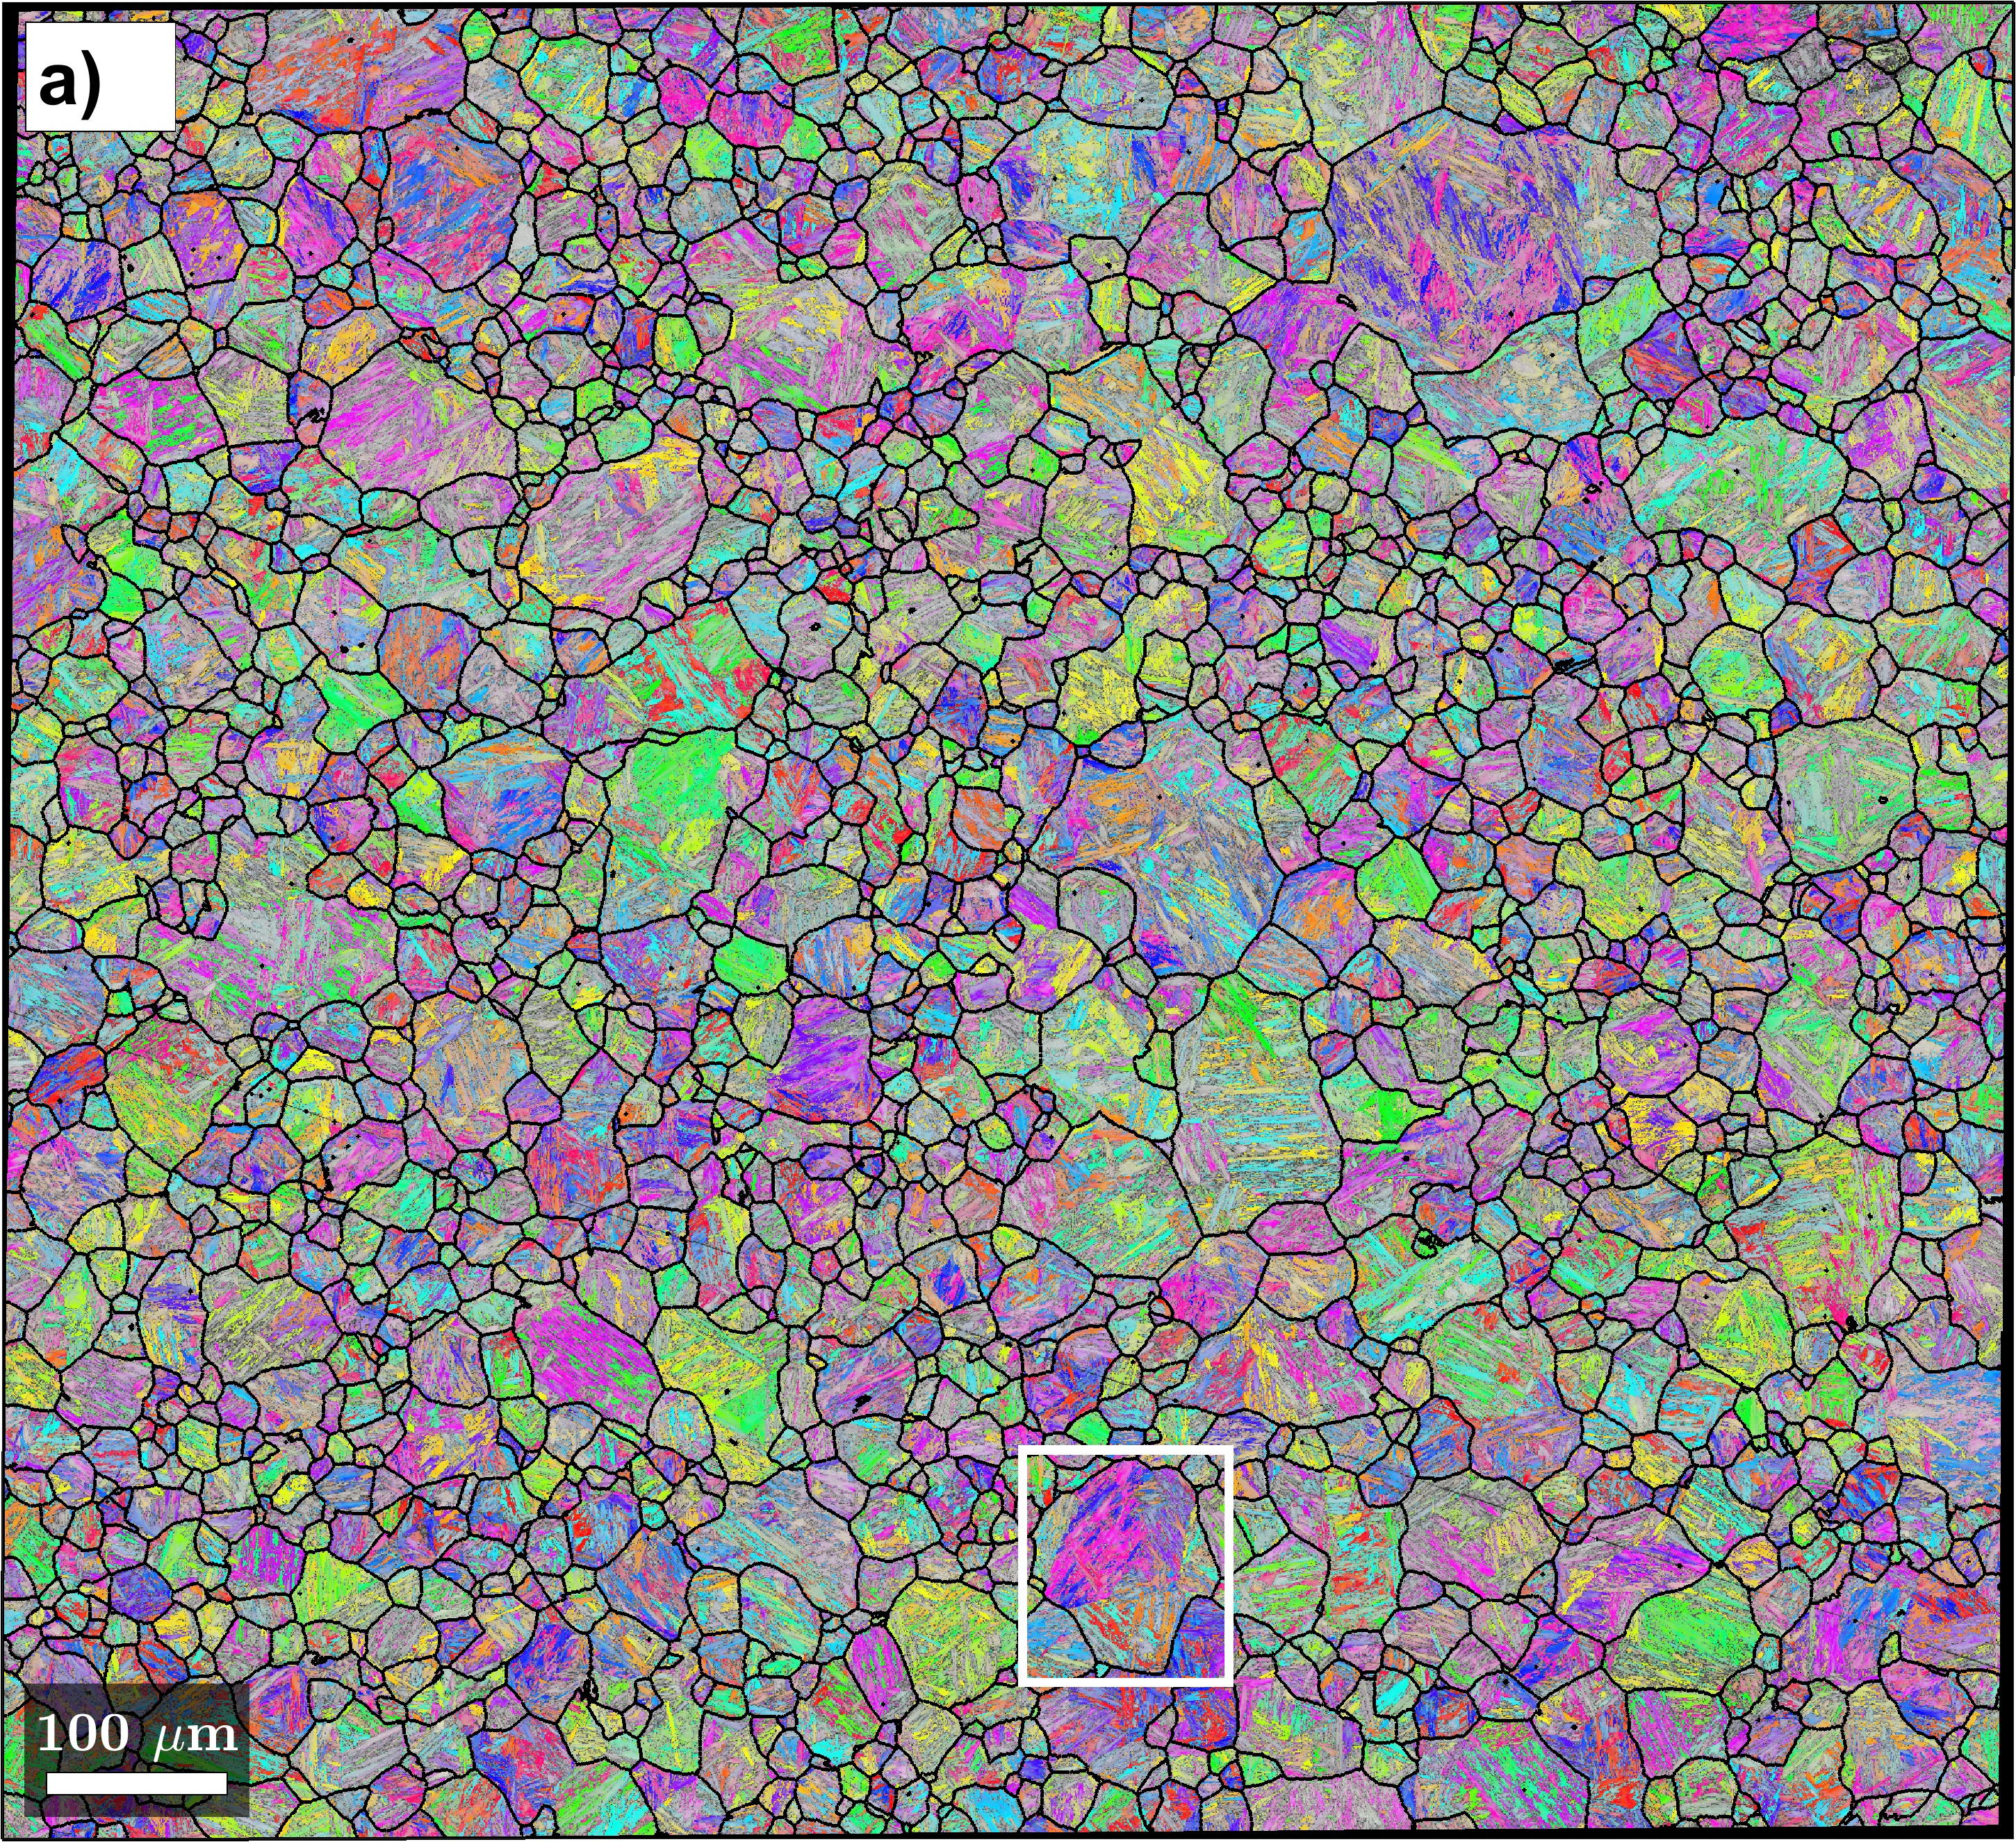
\includegraphics[width = \textwidth]{pic/grain_map_example_large.jpg}}
      \only<2>{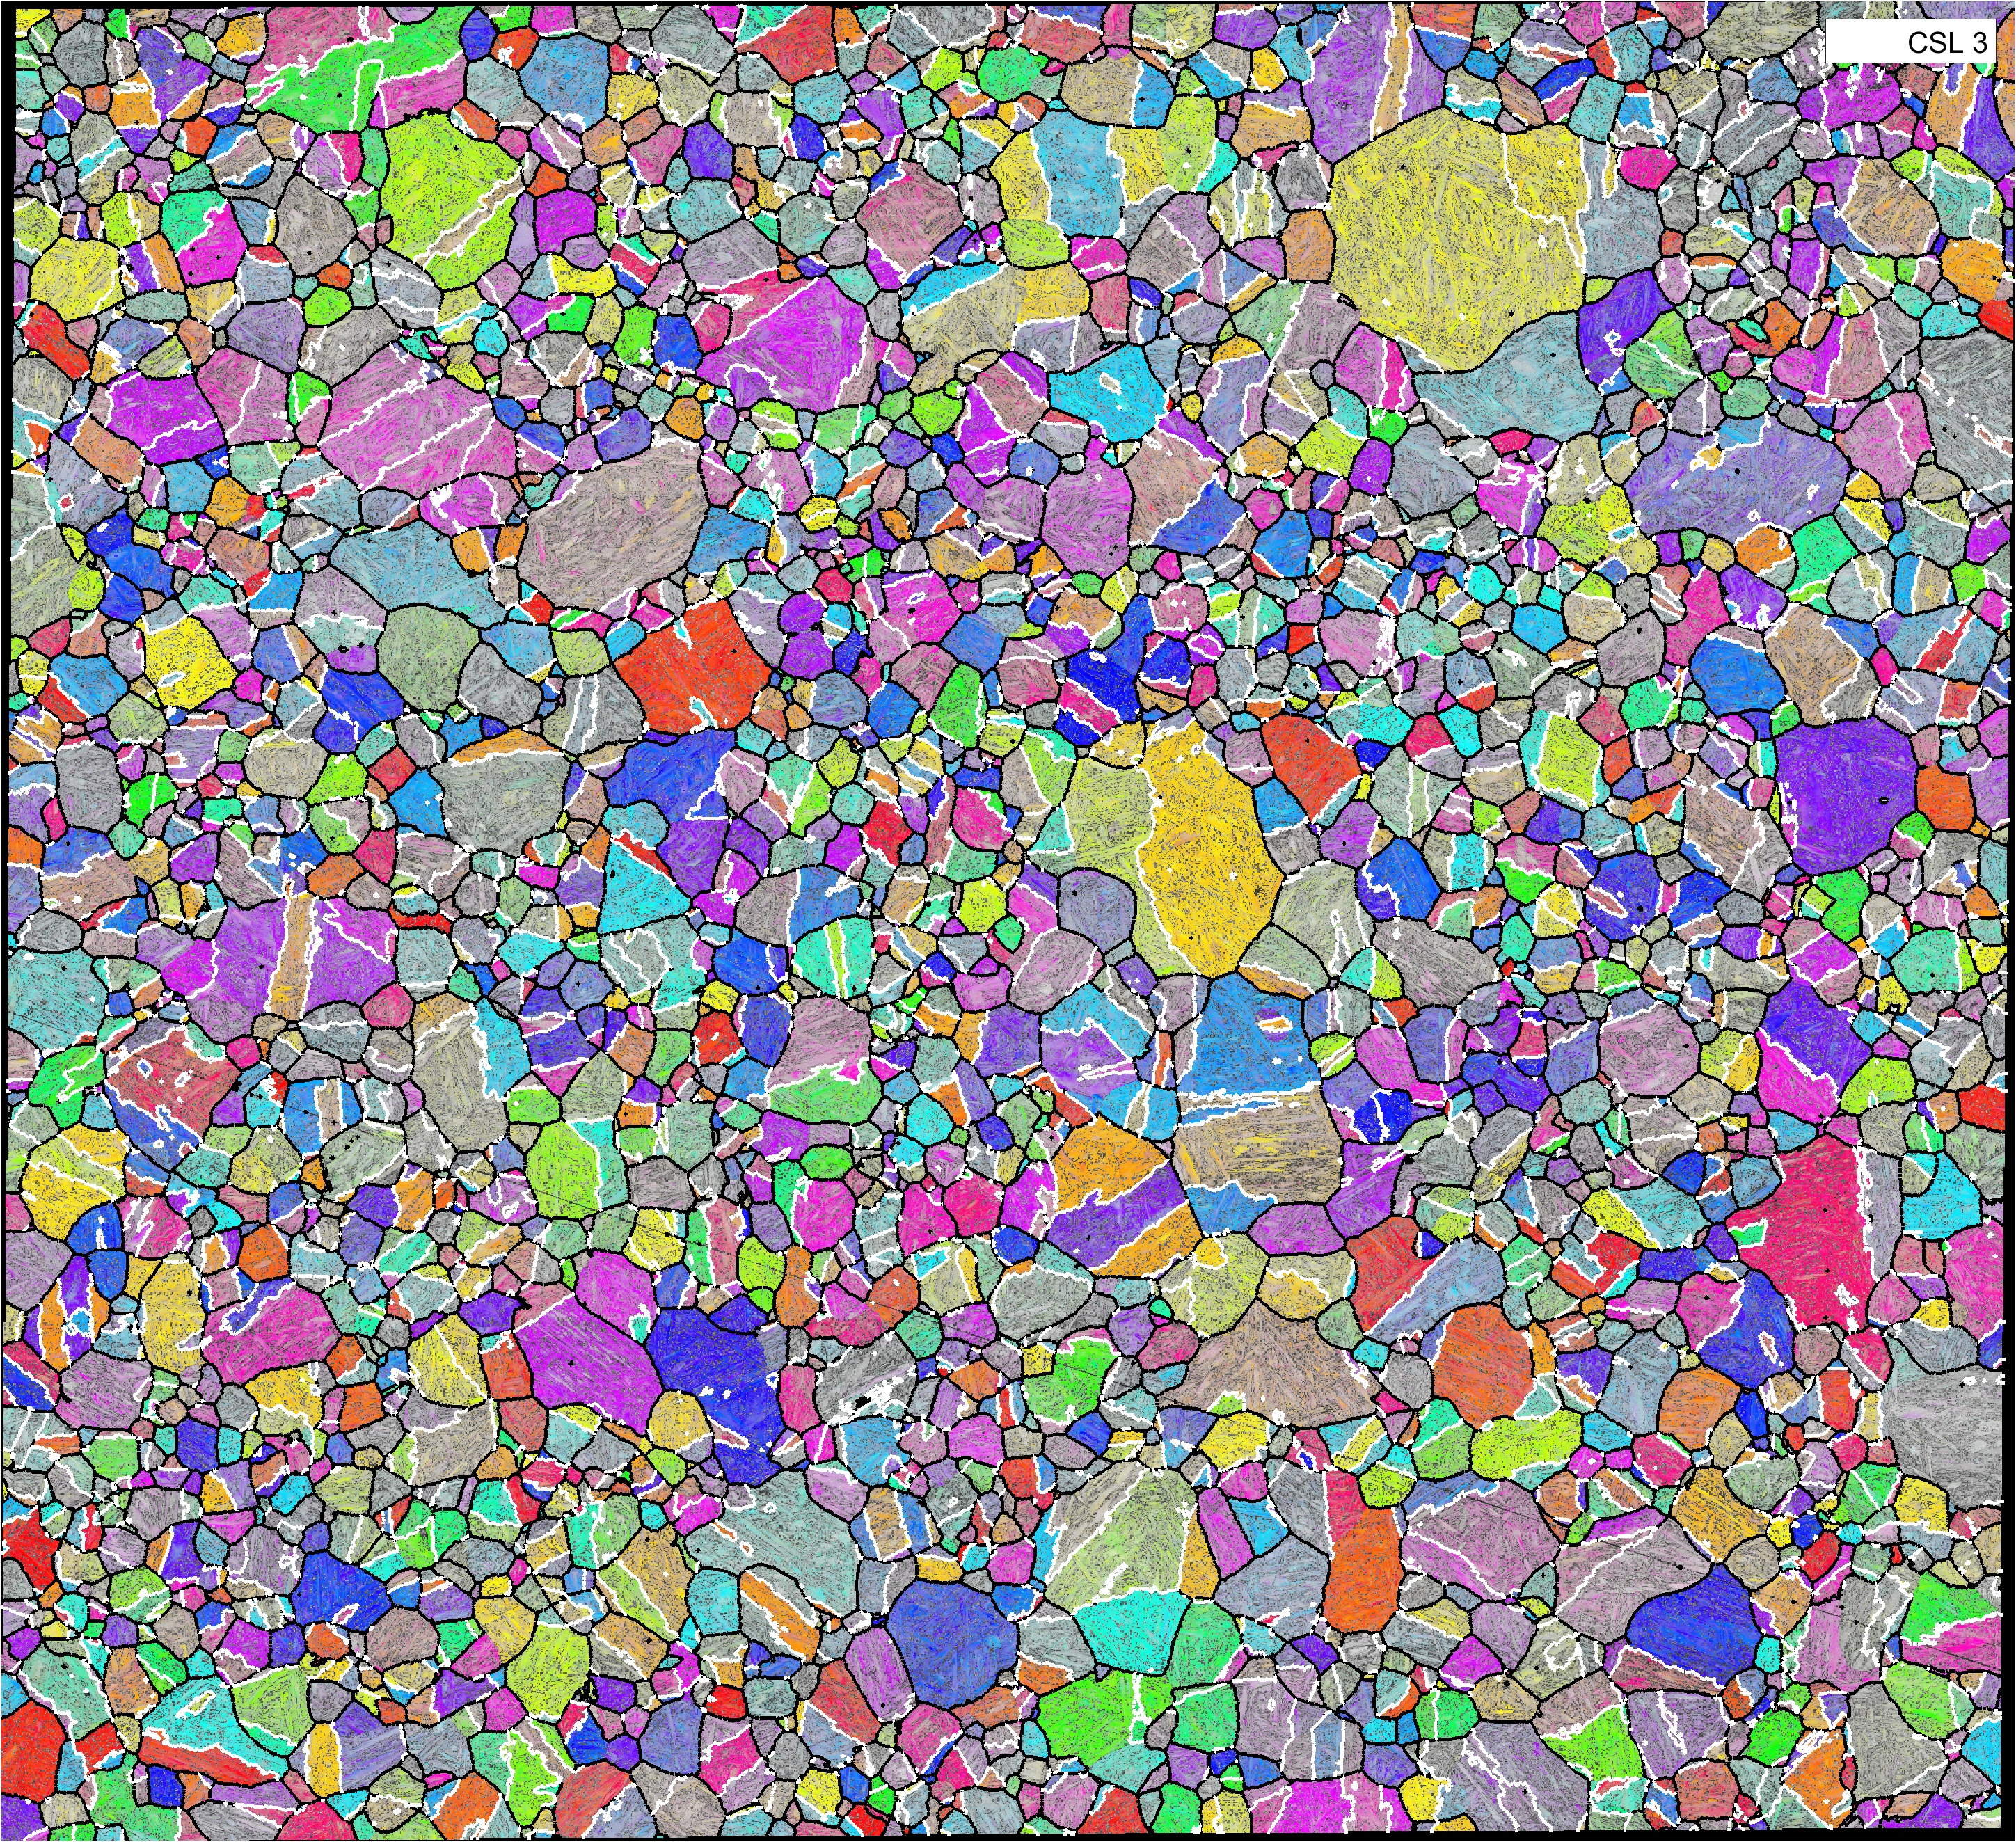
\includegraphics[width = \textwidth]{pic/large_austenite_map}}%
      
    \end{column}
    
  \end{columns}
  
  %\includegraphics{pic/large_ausenite_map}
\end{frame}


\begin{frame}

  \frametitle{Highlights of the MTEX Implementation}

  \begin{itemize}
  \item free and open-source
  \item fast
  \item works for all OR-based phase transformations
  \item works for multi-step phase transformations
  \item includes many different parent grain reconstruction methods
  \item modular design allows for the combination of different
    methods
  \item keeps track of the parent to child grain relationship trough the
    entire reconstruction process
  \item allows for the conditional reversion of reconstructed parent grains
  \item allows for of geometrical criteria
  \item its fun to play with
  \item addon OR Tools (https://github.com/frankNiessen/ORTools) provide extended functionality
  \end{itemize}

  \pause
  \bigskip

\begin{center}
  \Huge Thank you for your attention!
\end{center}


\end{frame}


\end{document}



\end{document}
\section{Three Data Sets}

\begin{frame}
  \frametitle{The Emsland Meteorite}

  \begin{columns}[T,onlytextwidth]
    \begin{column}{0.5\textwidth}
      \begin{overlayarea}{\textwidth}{0.9\textheight}
        \begin{itemize}
        \item<1-> found 1940 in a moor in Lower Saxony
        \item<1-> 19kg, 22 × 19 × 13cm
        \item<2-> 87\% Ferrit, 13\% Austenit
        \item<2-> data by Gert Nolze
        \item<3-> all Austenite from one prior grain
        \item<4-> Ferrite has very specific texture 
        \end{itemize}

        \bigskip

        \begin{center}
          \only<3>{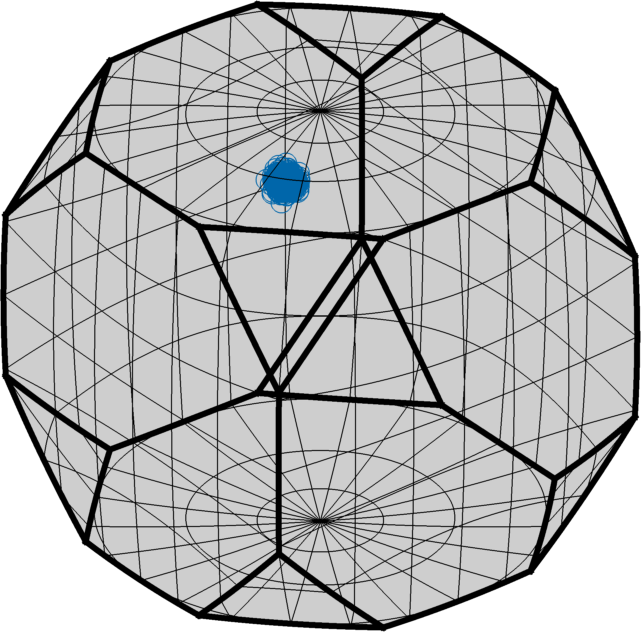
\includegraphics[width=4.5cm]{pic/oriParent}}
          \only<4>{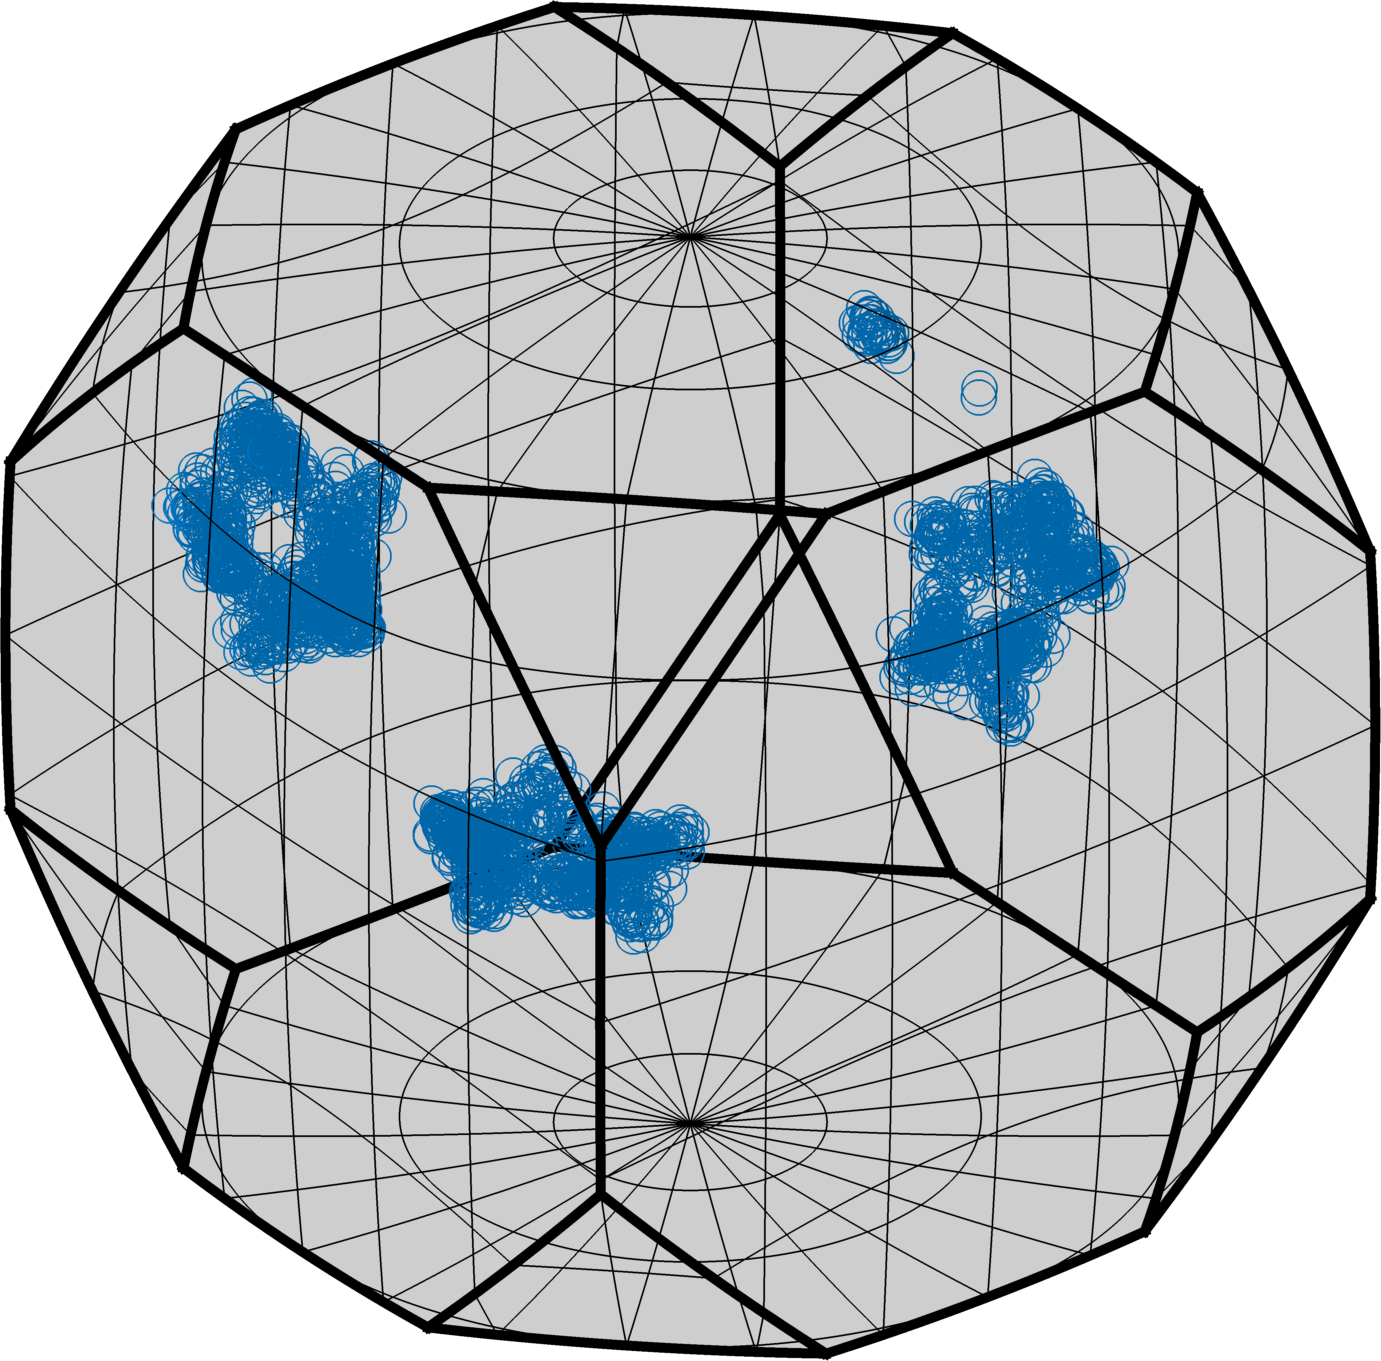
\includegraphics[width=4.5cm]{pic/oriChild}}
        \end{center}
      \end{overlayarea}
    \end{column}
    \begin{column}{0.45\textwidth}
      \begin{overlayarea}{\textwidth}{0.9\textheight}
        \begin{center}
          \only<1>{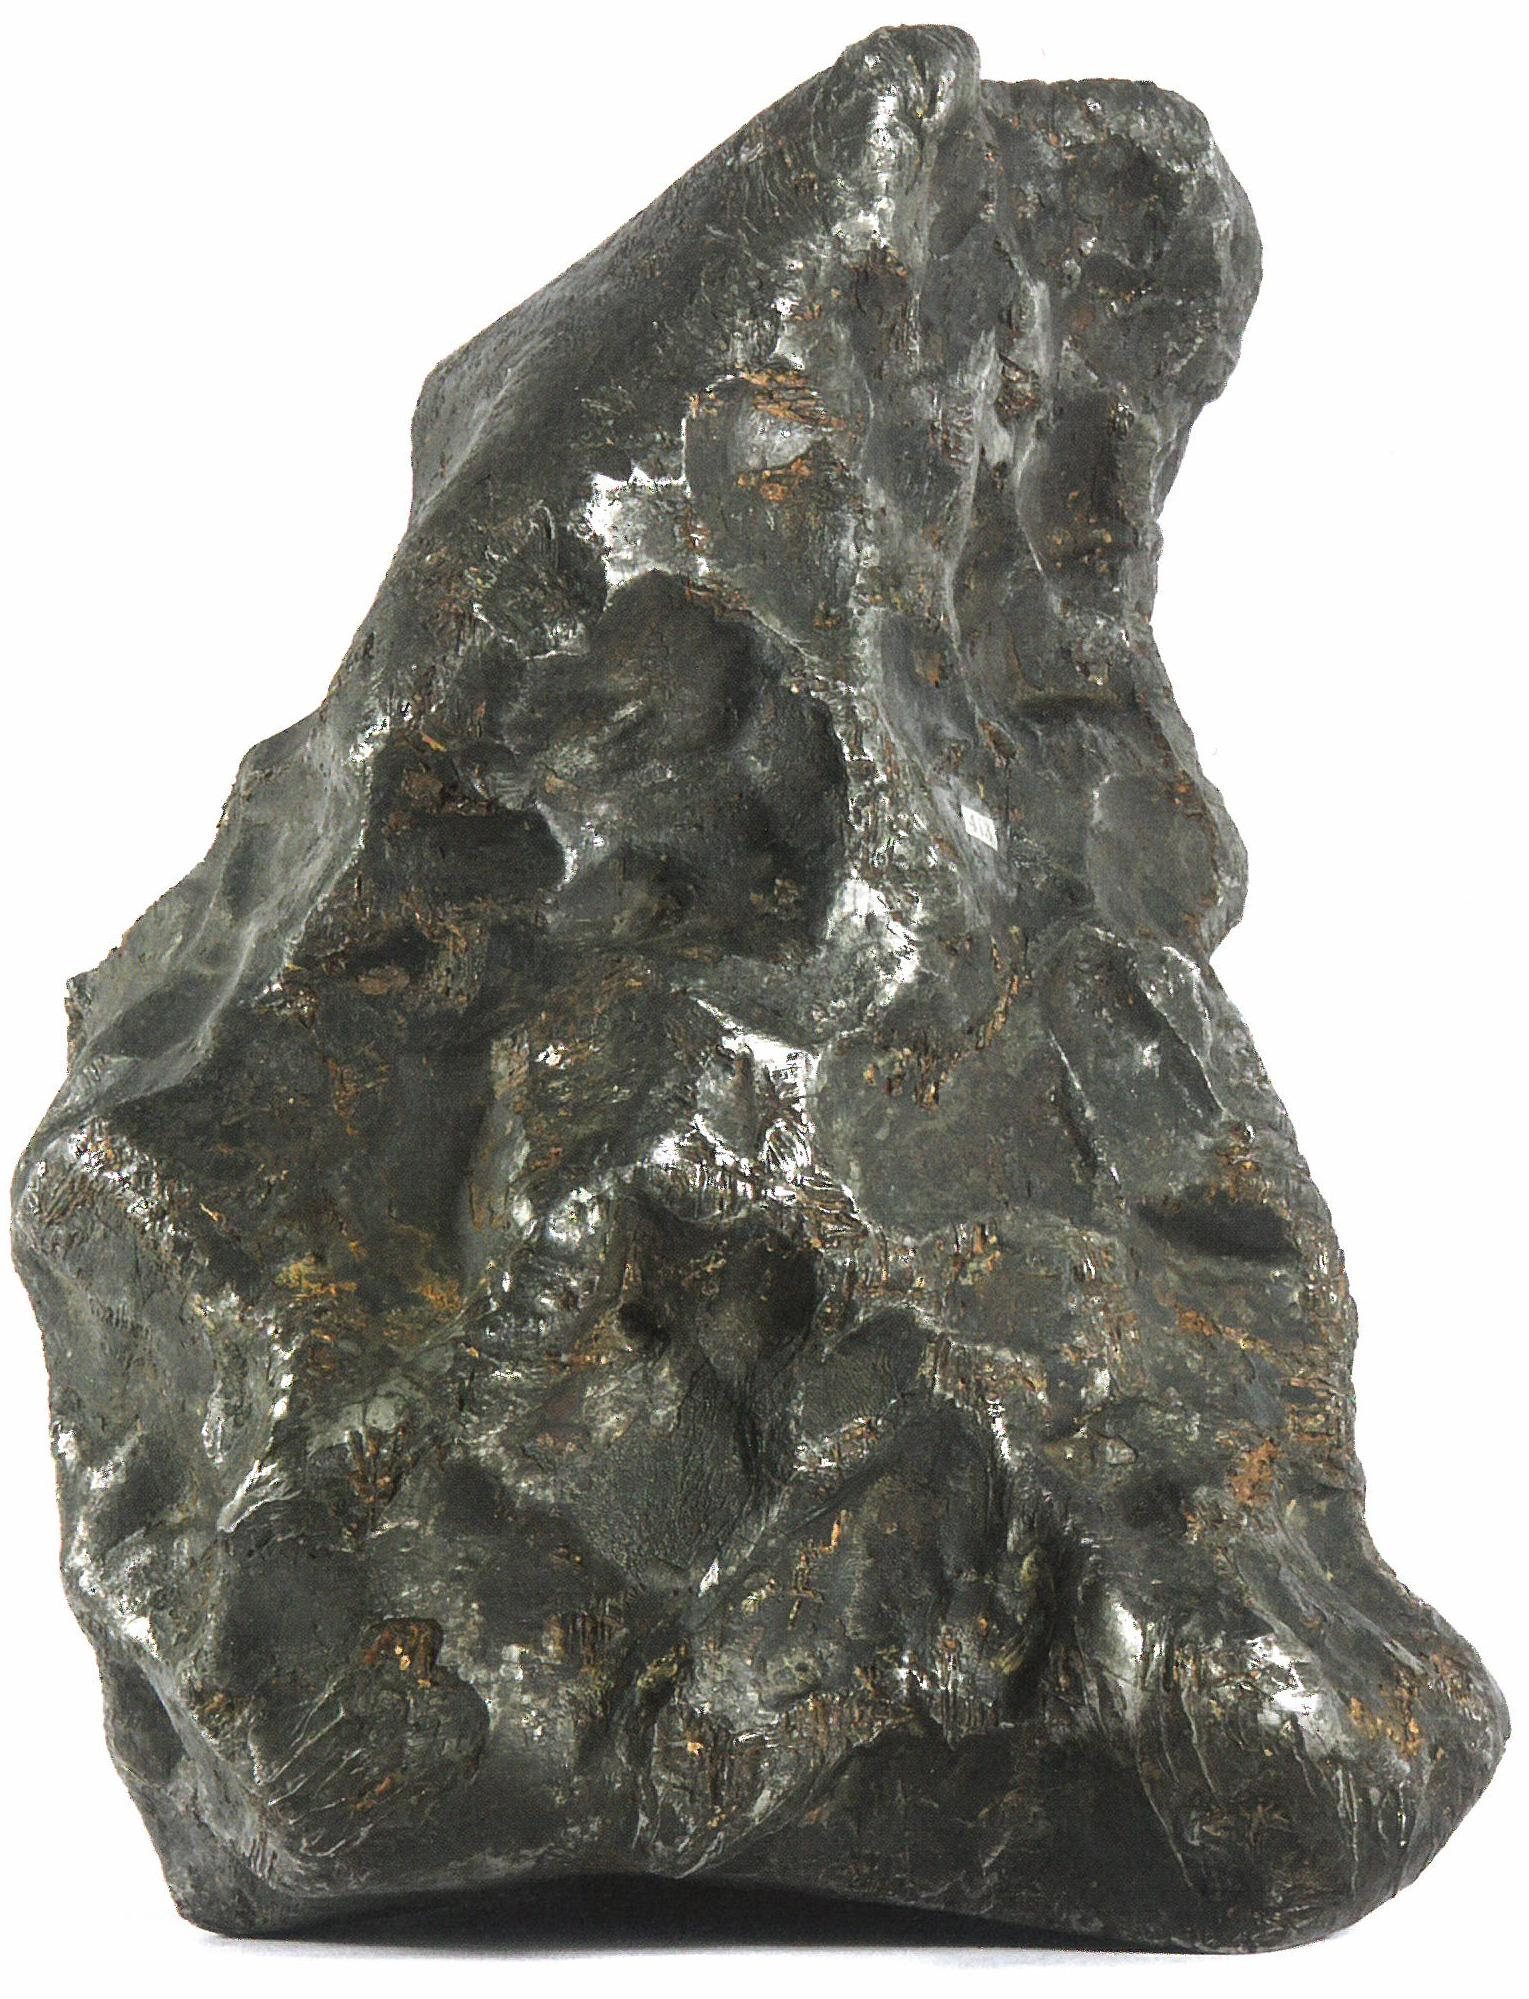
\includegraphics[width=0.8\textwidth]{pic/emslandMetereoit}\vspace{0.5cm}\
          }
          \only<2->{%
            \vspace{-1cm}%
            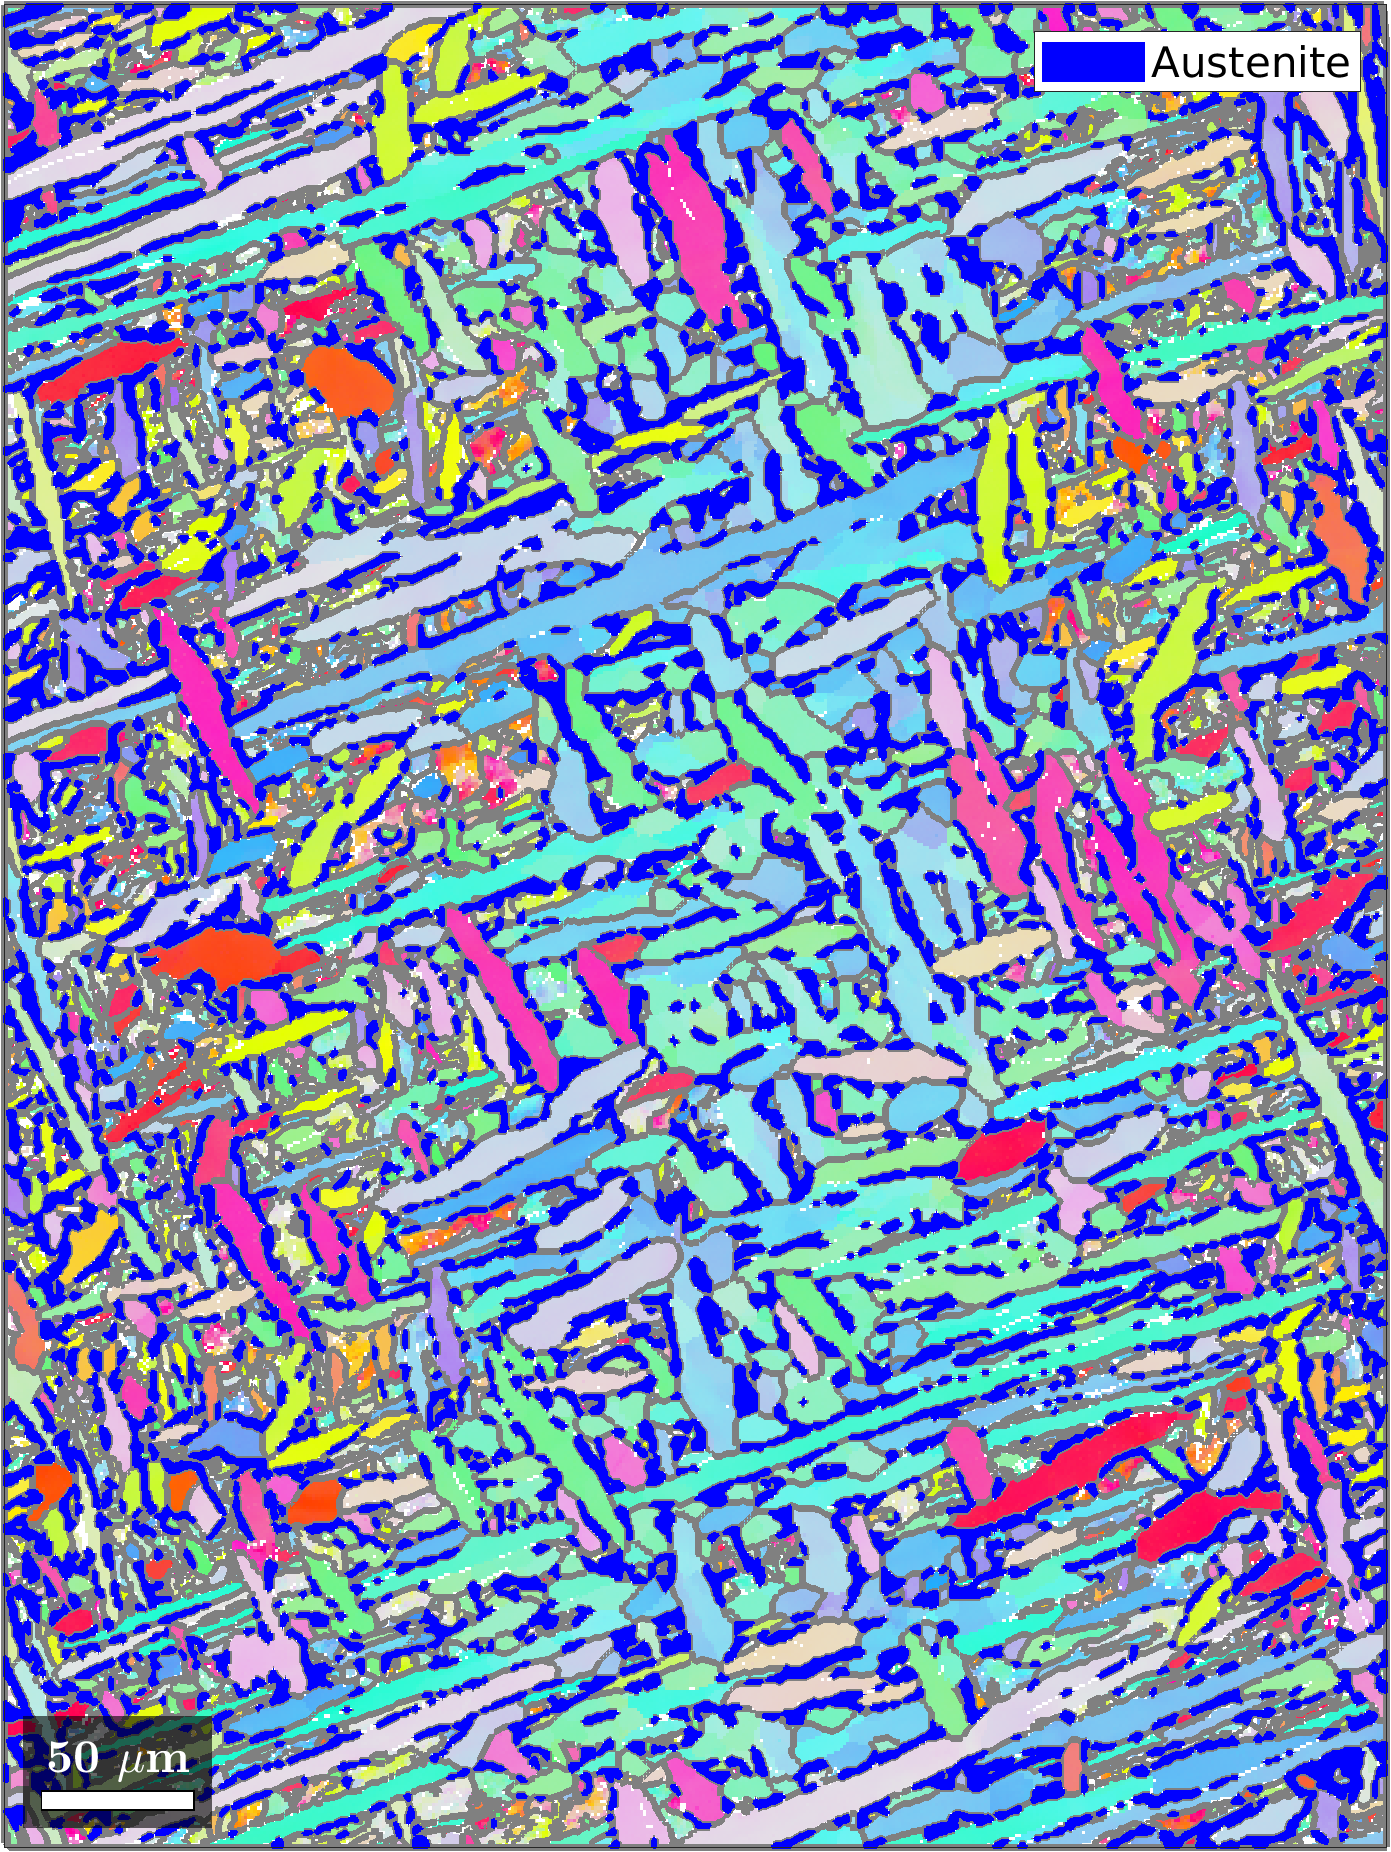
\includegraphics[height=0.95\textheight]{pic/mapFerrite}\vspace{0.5cm}\
          }
        \end{center}
      \end{overlayarea}
    \end{column}
  \end{columns}
\end{frame}

\begin{frame}
  \frametitle{A Titanium Alloy}

\begin{columns}
    \begin{column}{0.55\textwidth}
      \begin{overlayarea}{\textwidth}{0.9\textheight}
        \begin{itemize}
        \item data courtesy: Susanne Hemes, Aachen
        \item 94\% alpha titanium
        \item 0.22 \% beta titanium
        \item 5.3\% not indexed
        \end{itemize}

        \bigskip

        \begin{center}
          \only<1>{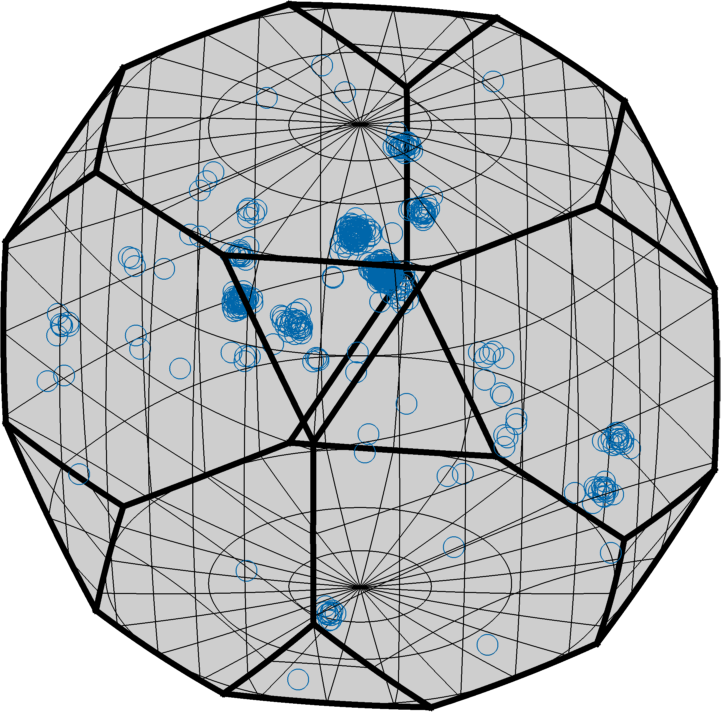
\includegraphics[width=4.5cm]{pic/TiOriBeta}}
        \end{center}
      \end{overlayarea}
    \end{column}
    \begin{column}{0.46\textwidth}
      \begin{overlayarea}{\textwidth}{0.9\textheight}
        \only<1>{\vspace{-0.9cm}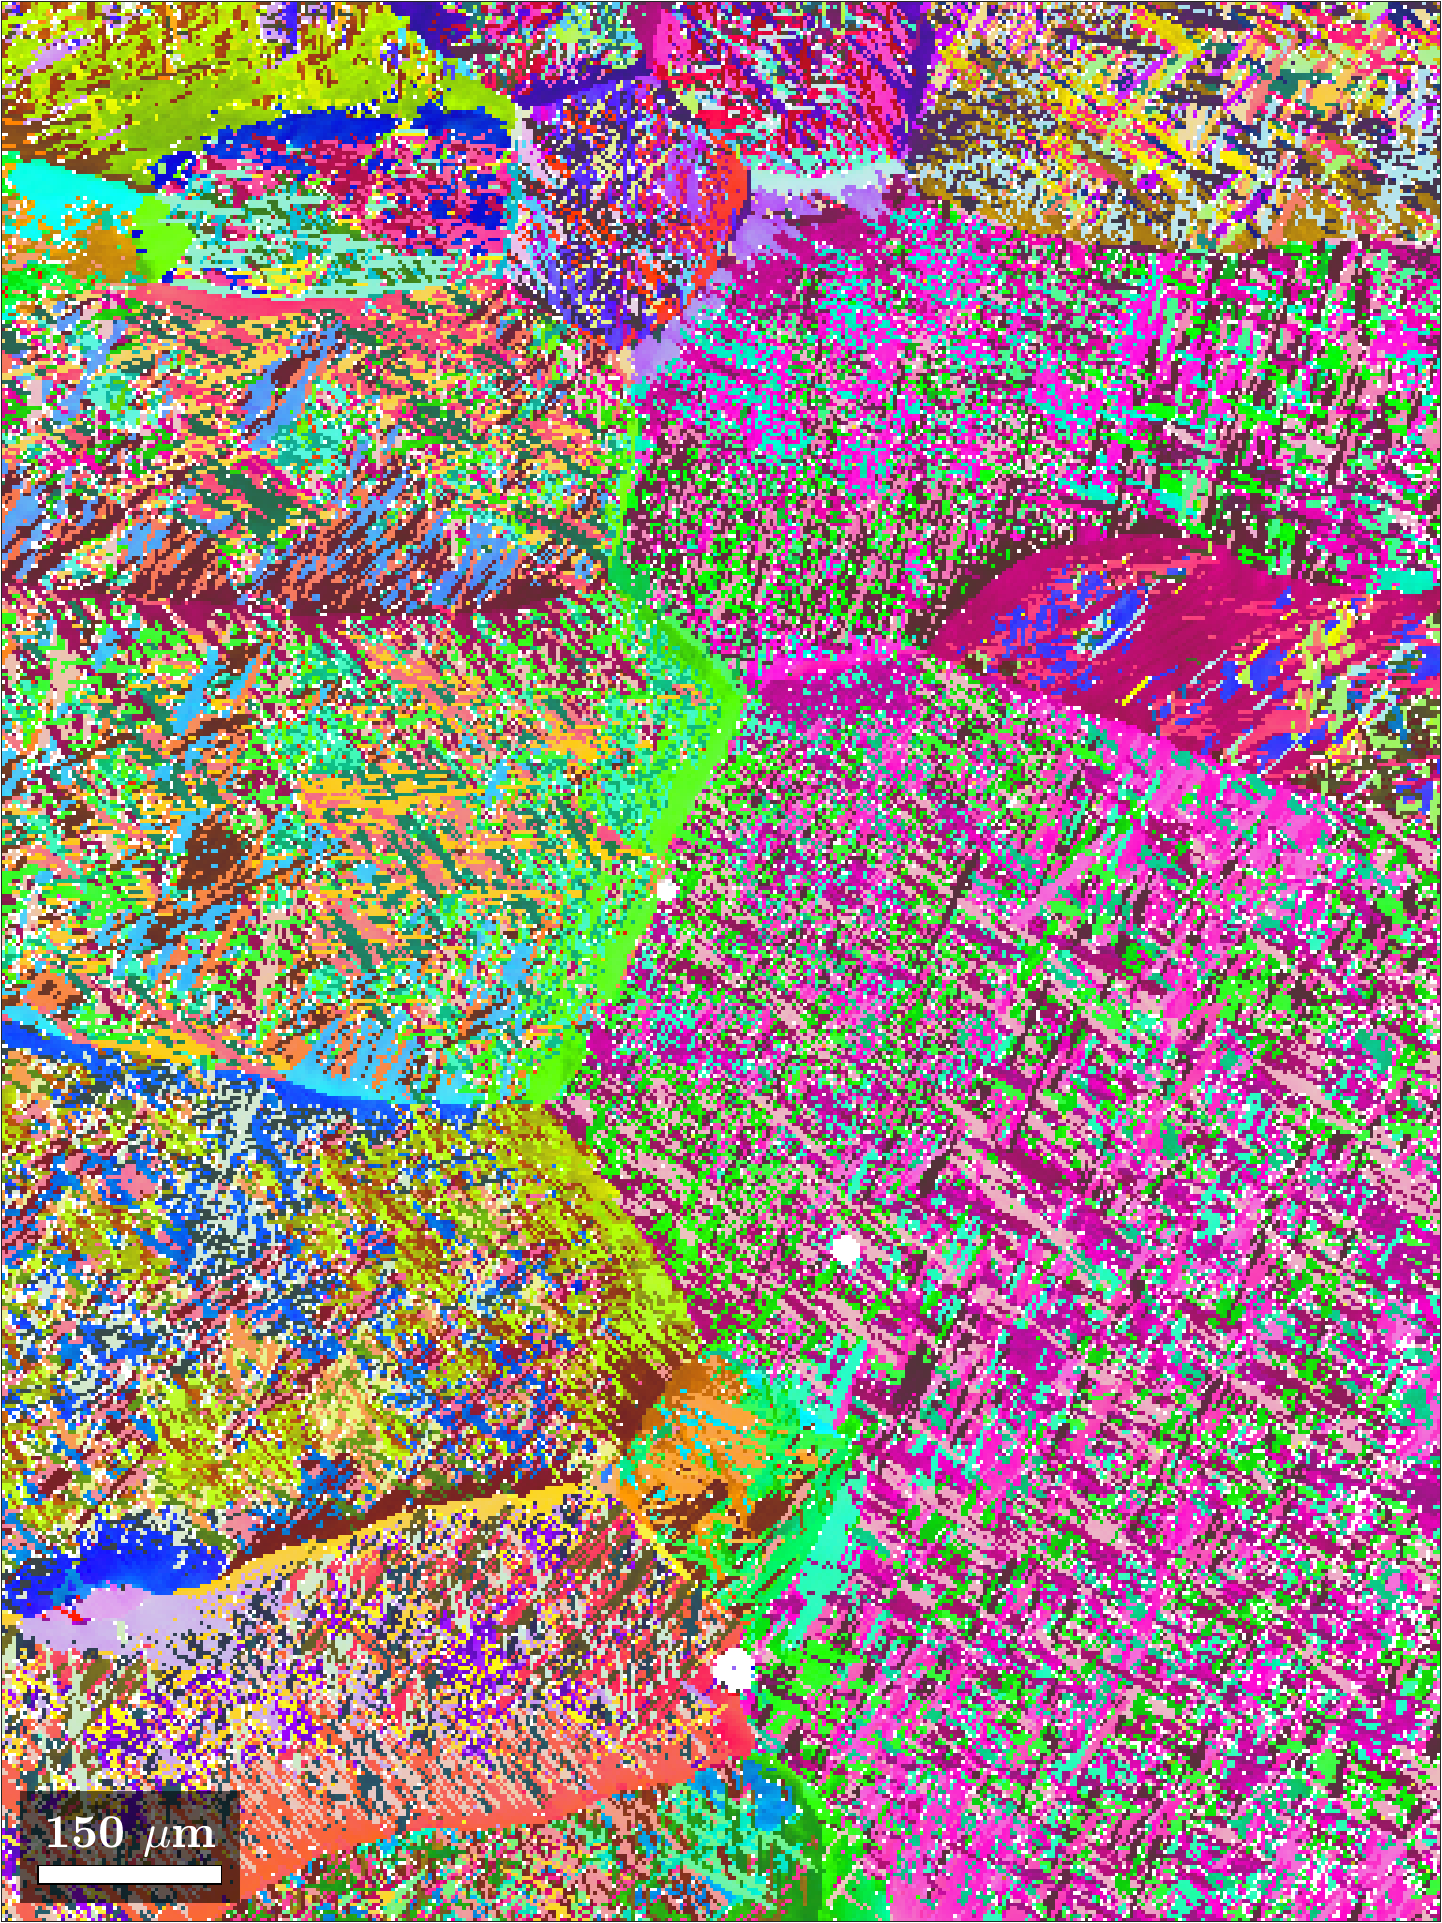
\includegraphics[width=\textwidth]{pic/TiMap}}
      \end{overlayarea}

    \end{column}
  \end{columns}

\end{frame}

\begin{frame}
  \frametitle{A Polycrystalline Austenite Alloy}

  \begin{columns}
    \begin{column}{0.55\textwidth}
      \begin{overlayarea}{\textwidth}{0.9\textheight}
        \begin{itemize}
        \item data courtesy: Tuomo Nyyssönen (Finnland)
        \item 71\% Austenite (bcc)
        \item 29\% not indexed
        \end{itemize}

        \bigskip

        \begin{center}
          \only<1>{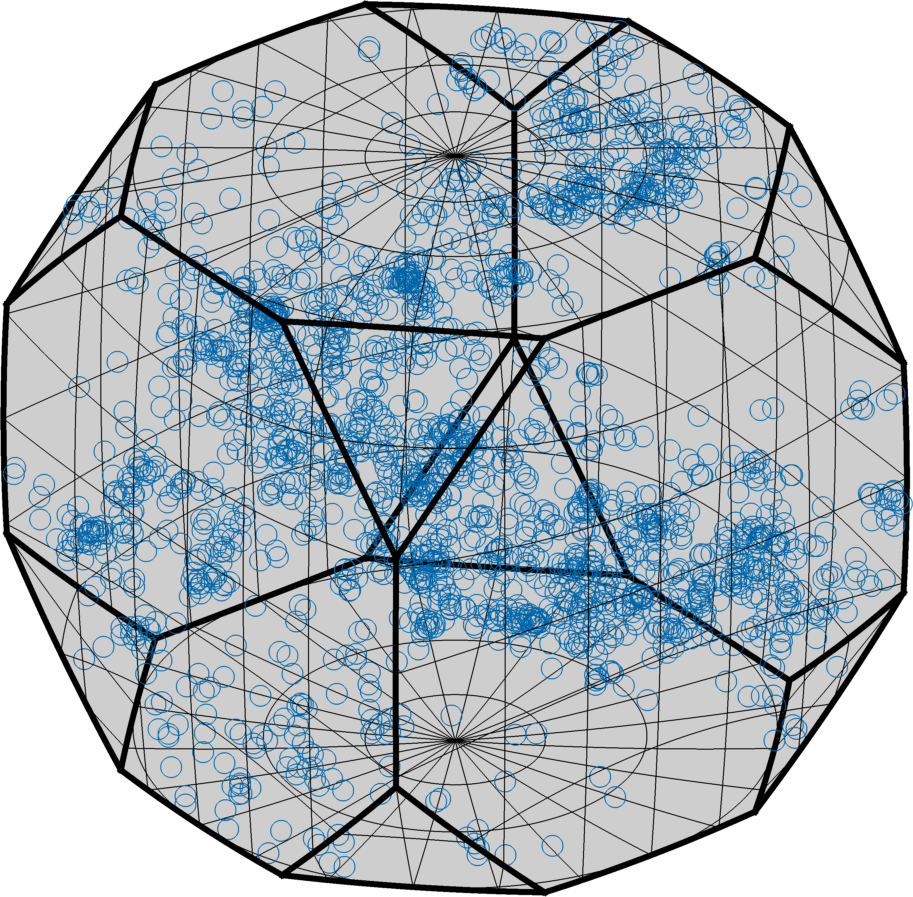
\includegraphics[width=4.5cm]{pic/MaOriBeta}}
        \end{center}
      \end{overlayarea}
    \end{column}
    \begin{column}{0.43\textwidth}
      \begin{overlayarea}{\textwidth}{1\textheight}
        \only<1>{\vspace{-0.9cm}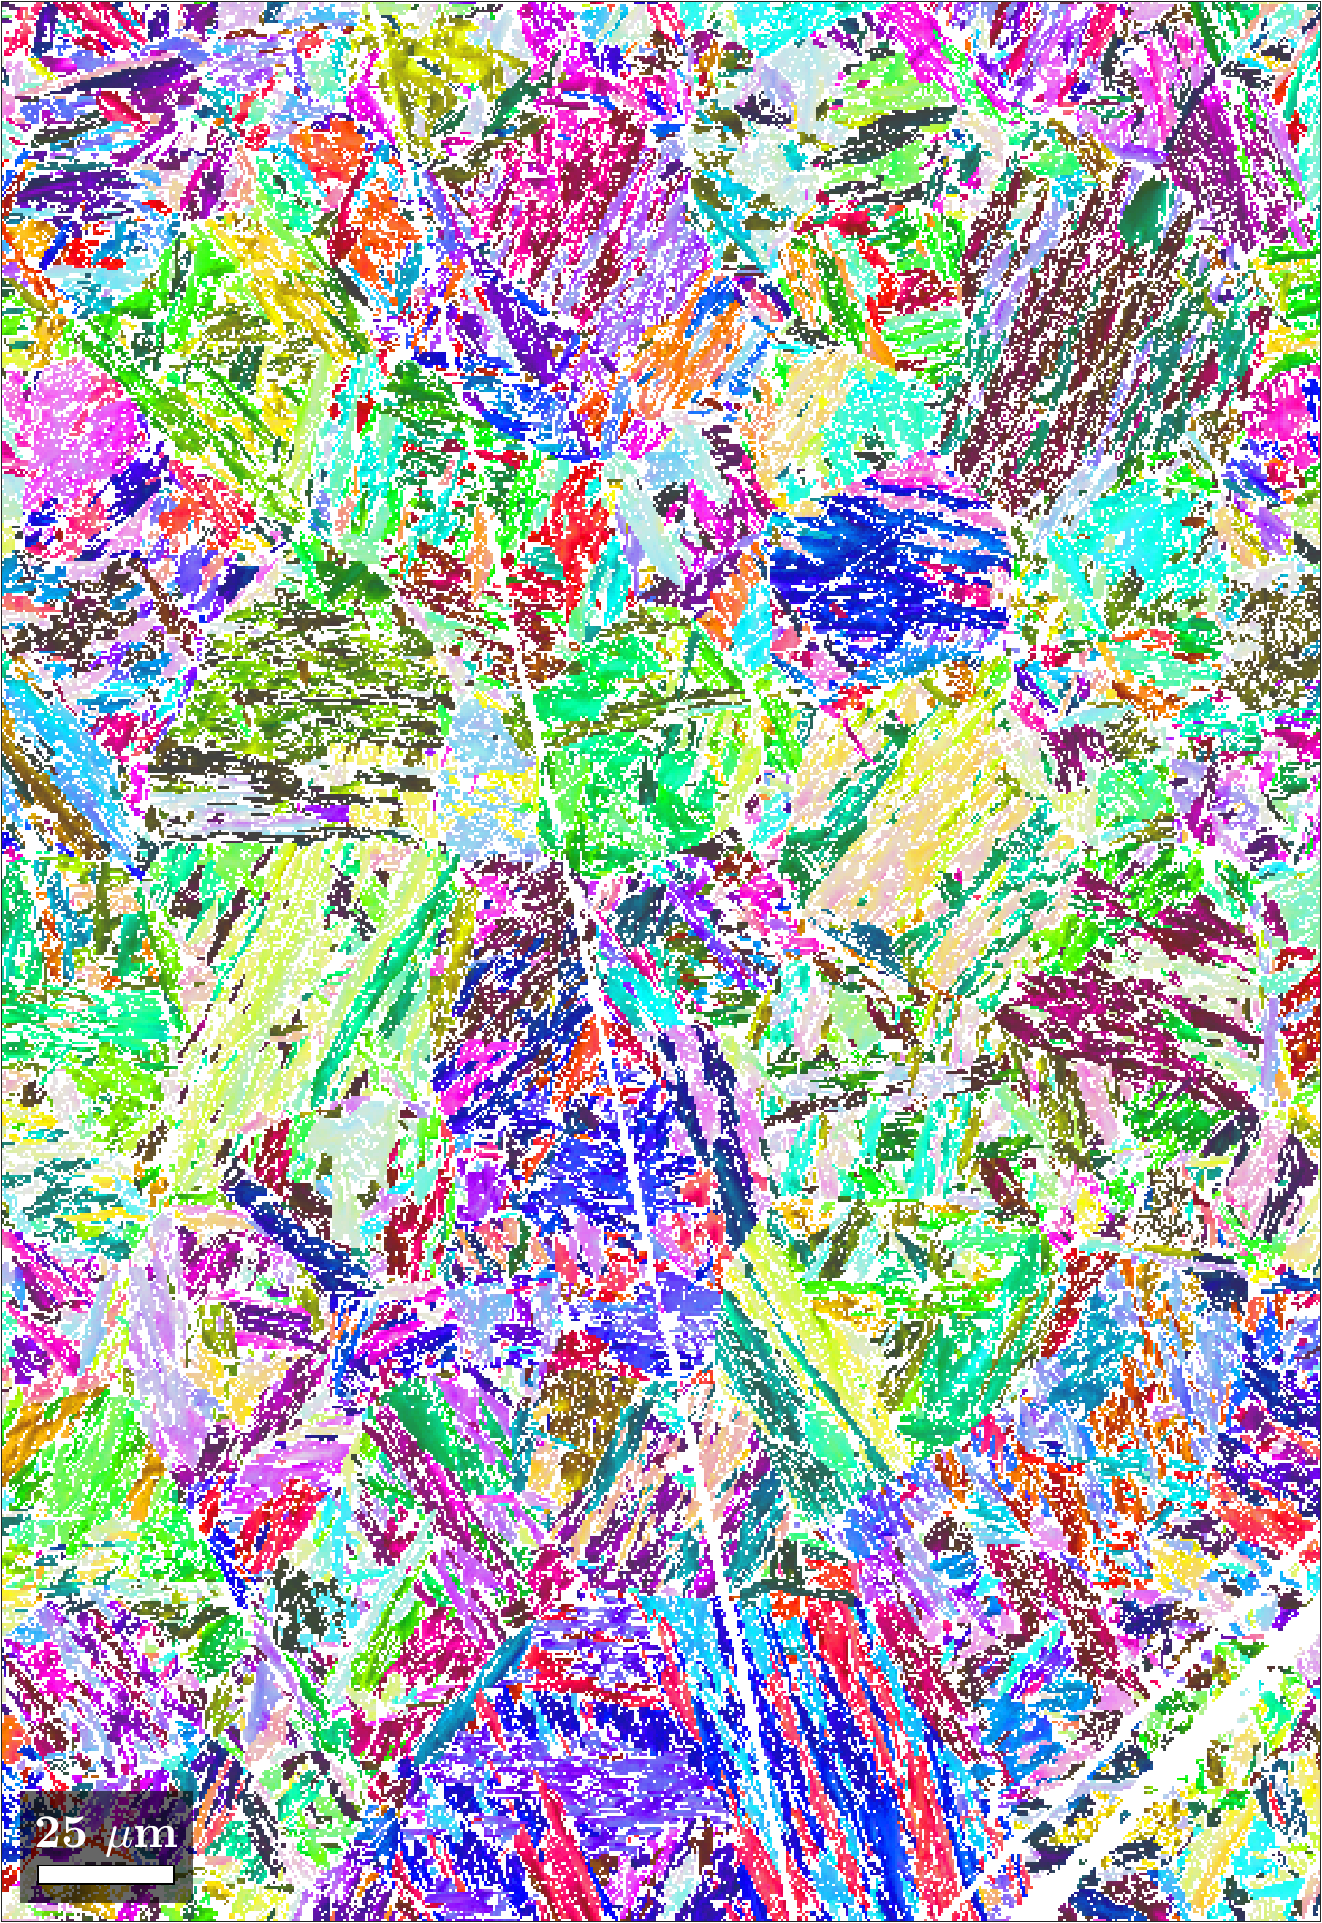
\includegraphics[width=\textwidth]{pic/MaData2}}
      \end{overlayarea}
    \end{column}
  \end{columns}

\end{frame}



\section{Determination of the Parent to Child Orientation Relationship}



\begin{frame}
\frametitle{Ferrite - Austenite Orientation Relationships}

\begin{center}
  \only<1>{\includegraphics[width=0.95\textwidth]{pic/pfSuperposed}}
  \only<2>{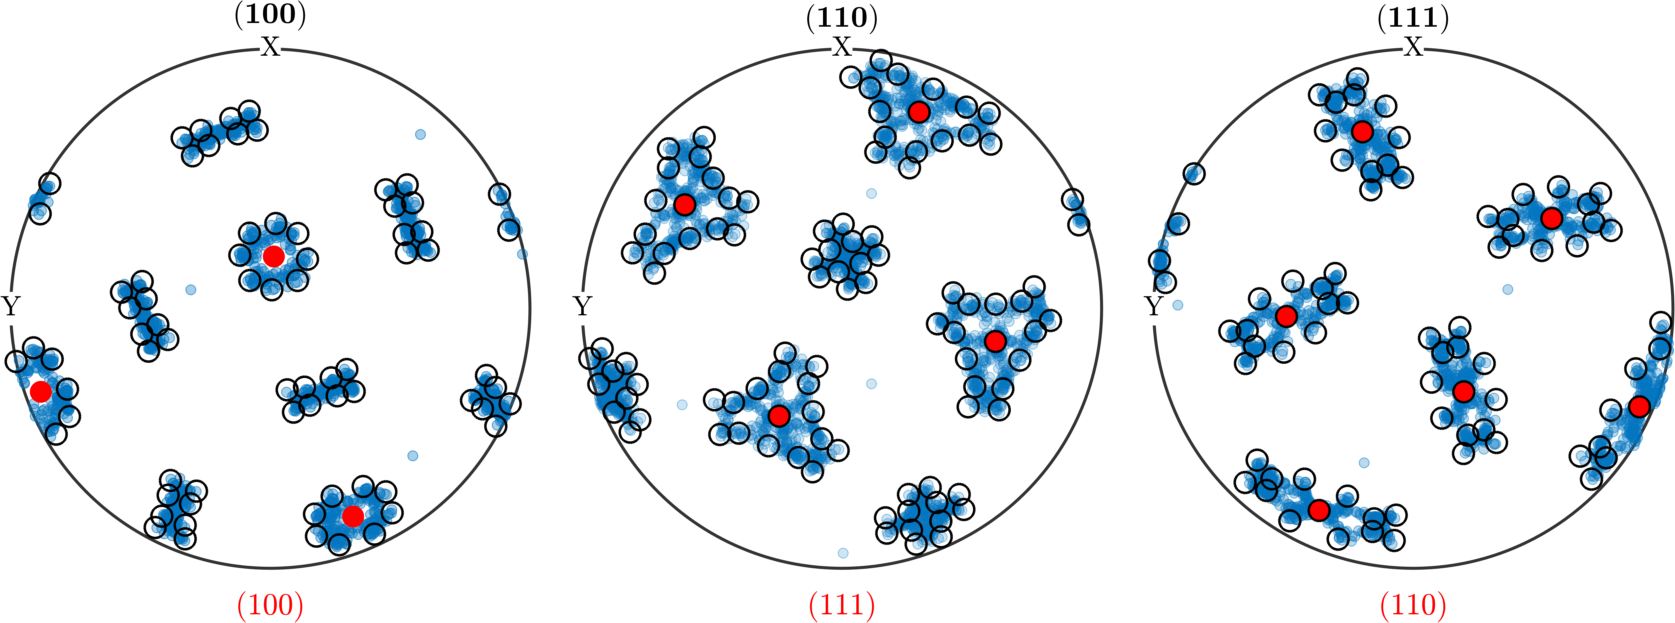
\includegraphics[width=0.95\textwidth]{pic/pfKS}}
  \only<3>{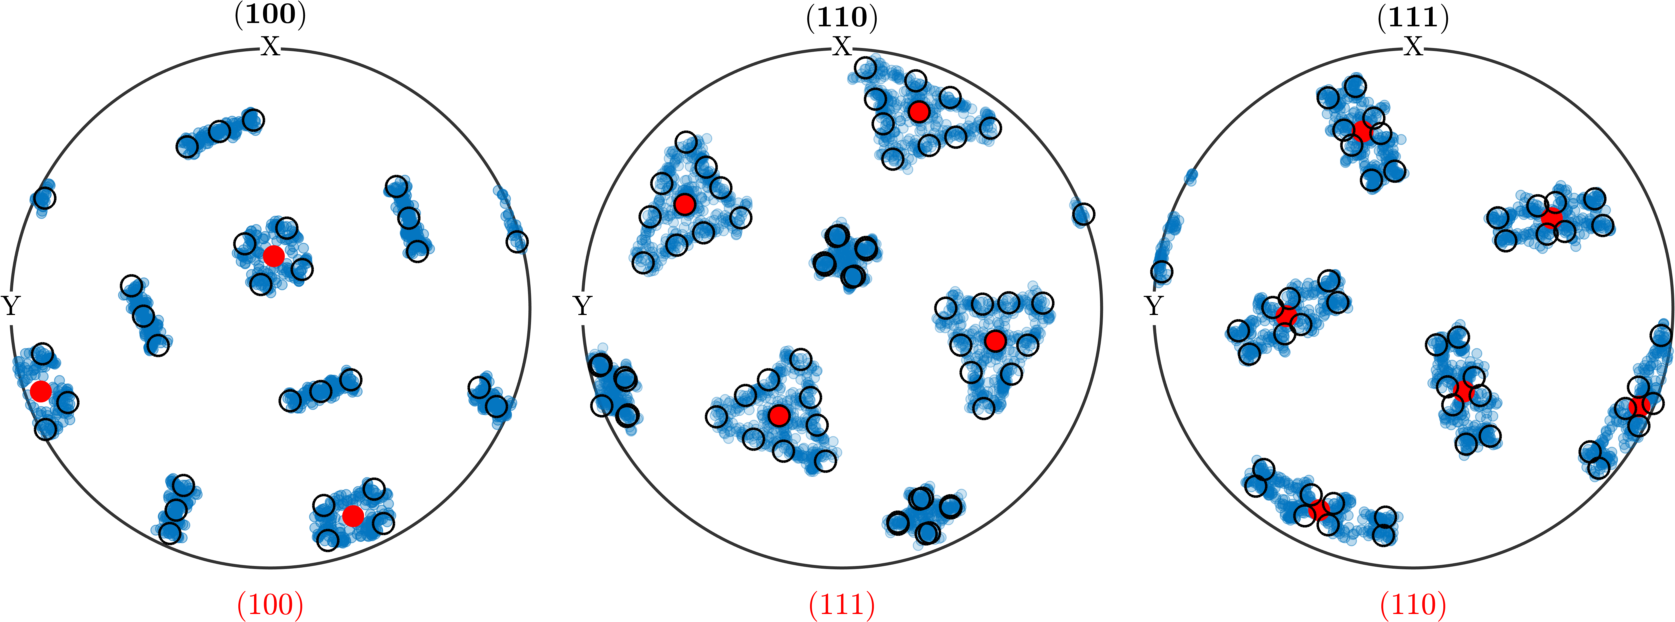
\includegraphics[width=0.95\textwidth]{pic/pfNW}}
  \only<4>{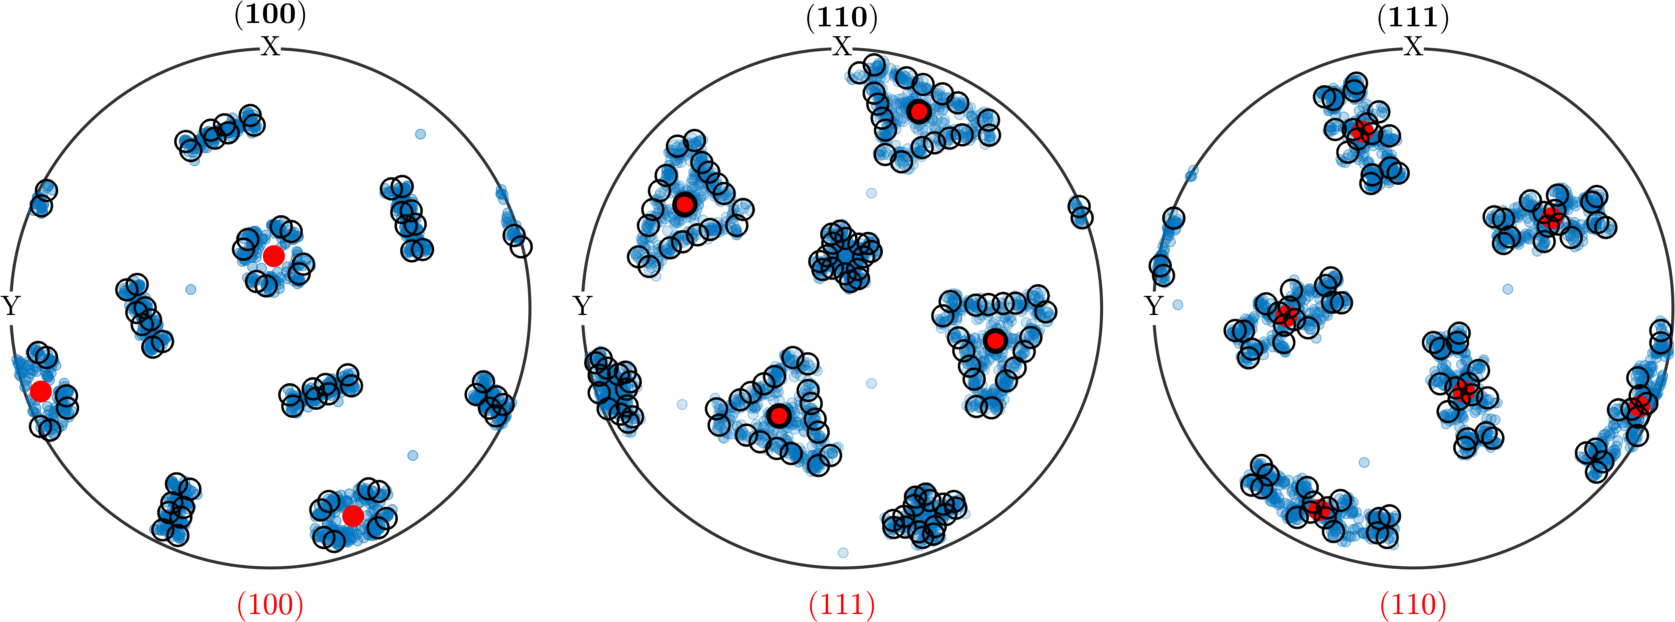
\includegraphics[width=0.95\textwidth]{pic/pfGT}}
  % \only<5>{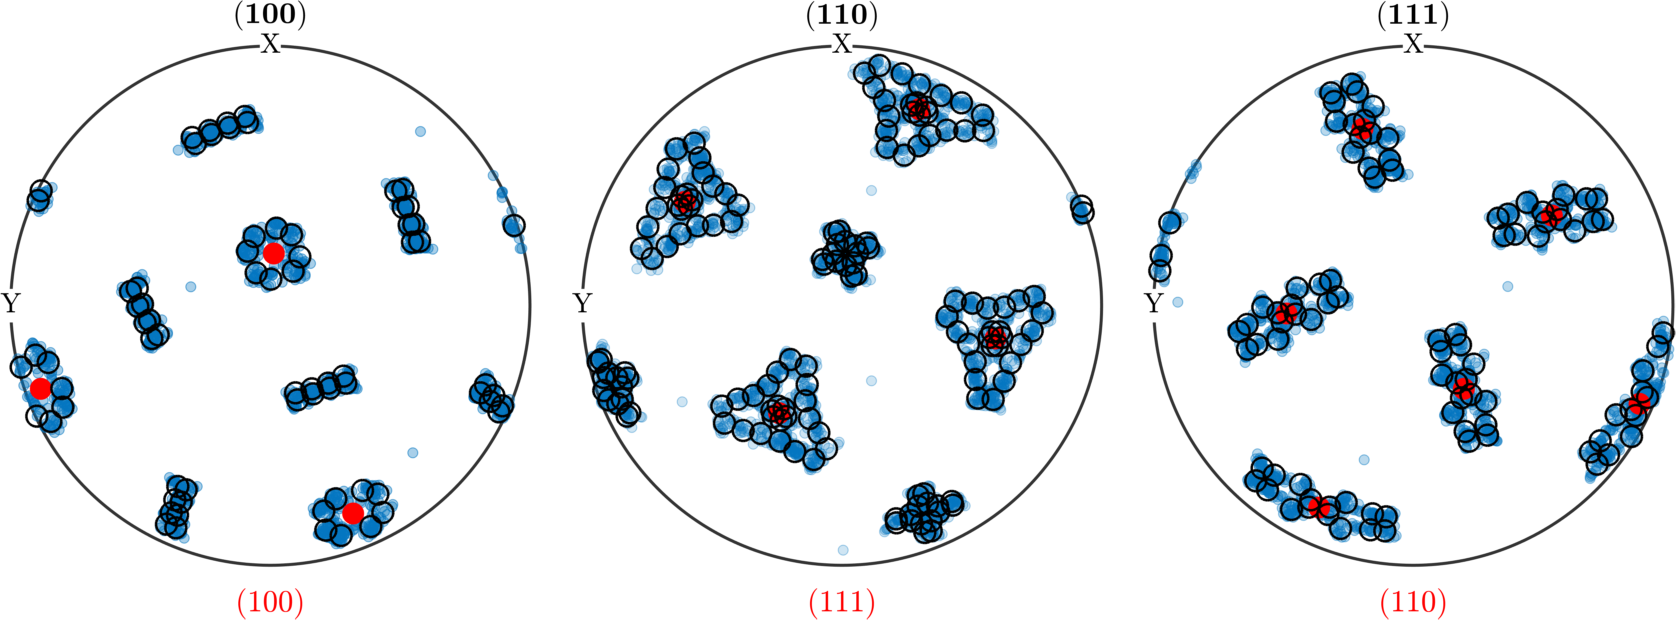
\includegraphics[width=\textwidth]{pic/pfMean}}
  % \only<6>{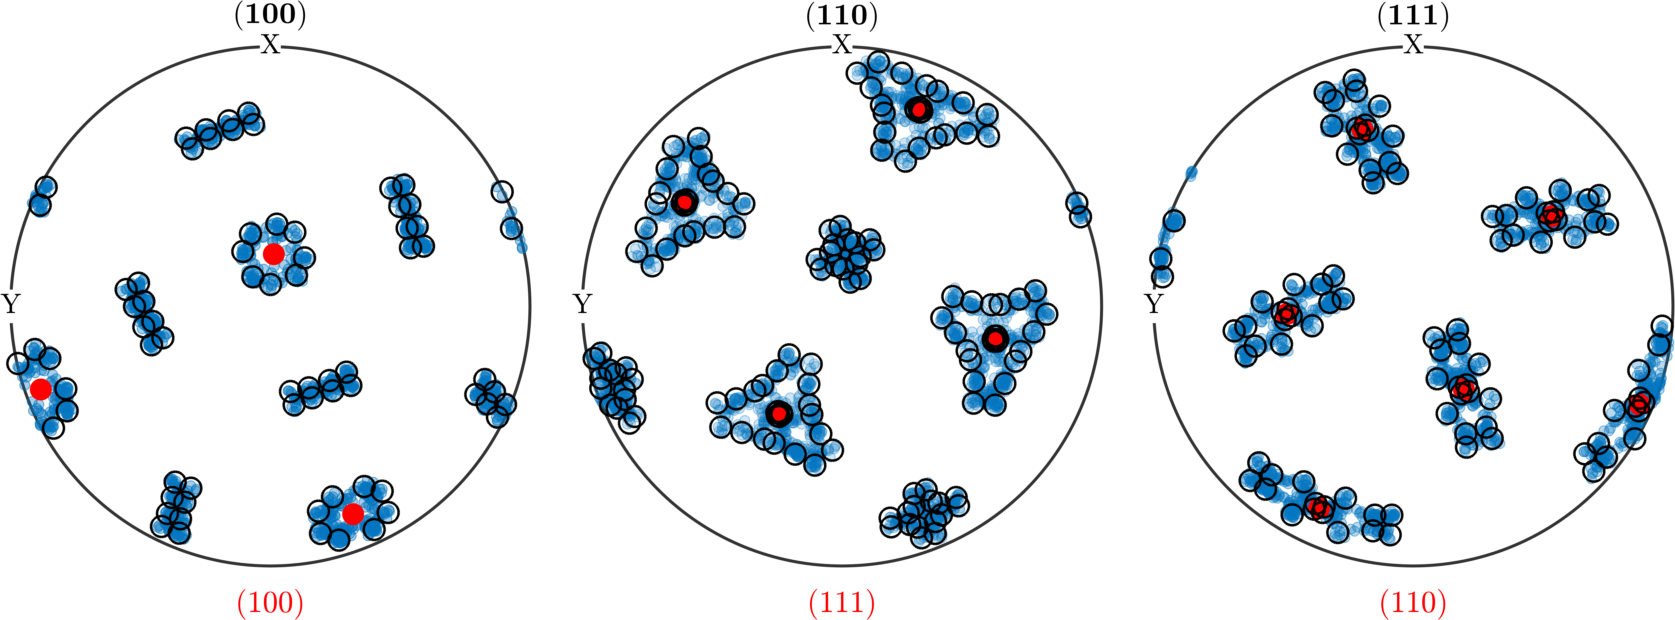
\includegraphics[width=\textwidth]{pic/pfMax}}
  % \only<7>{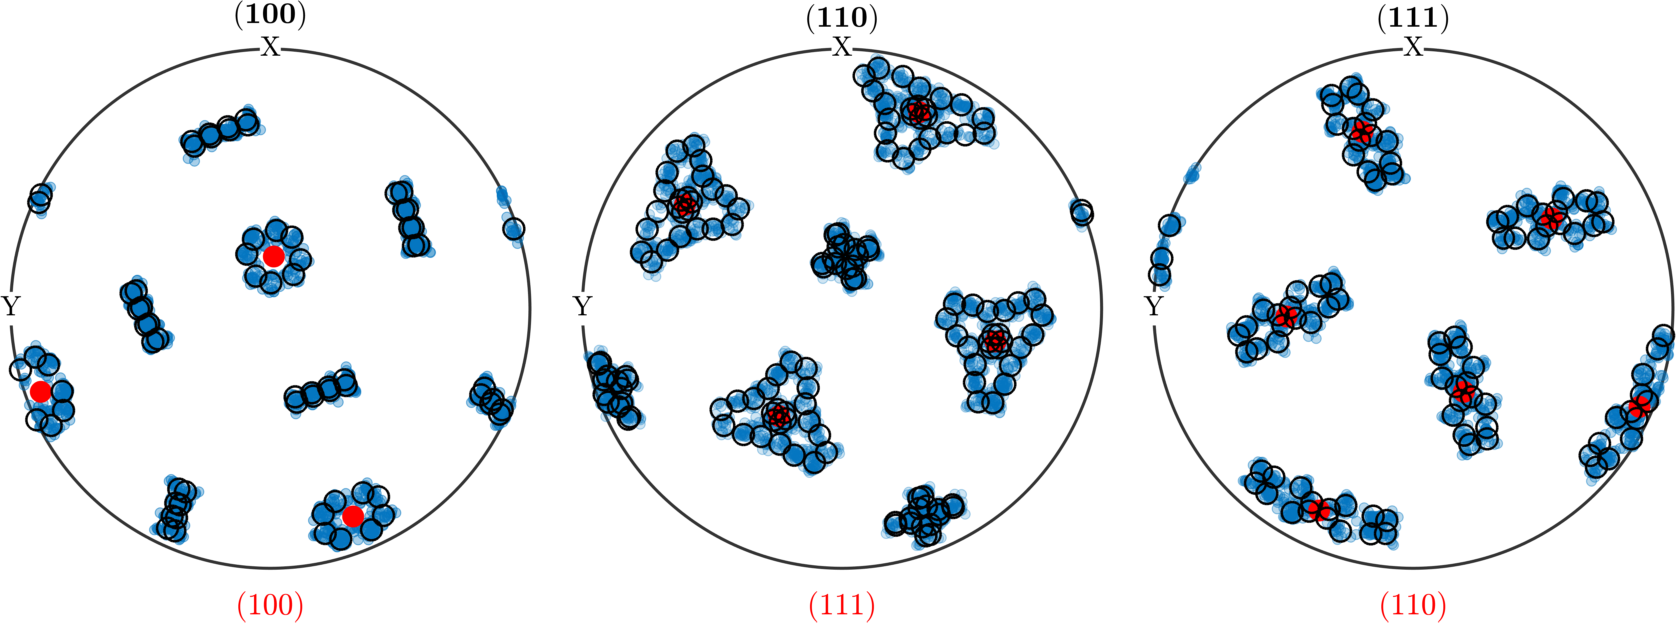
\includegraphics[width=\textwidth]{pic/pfIter}}
  % \only<8>{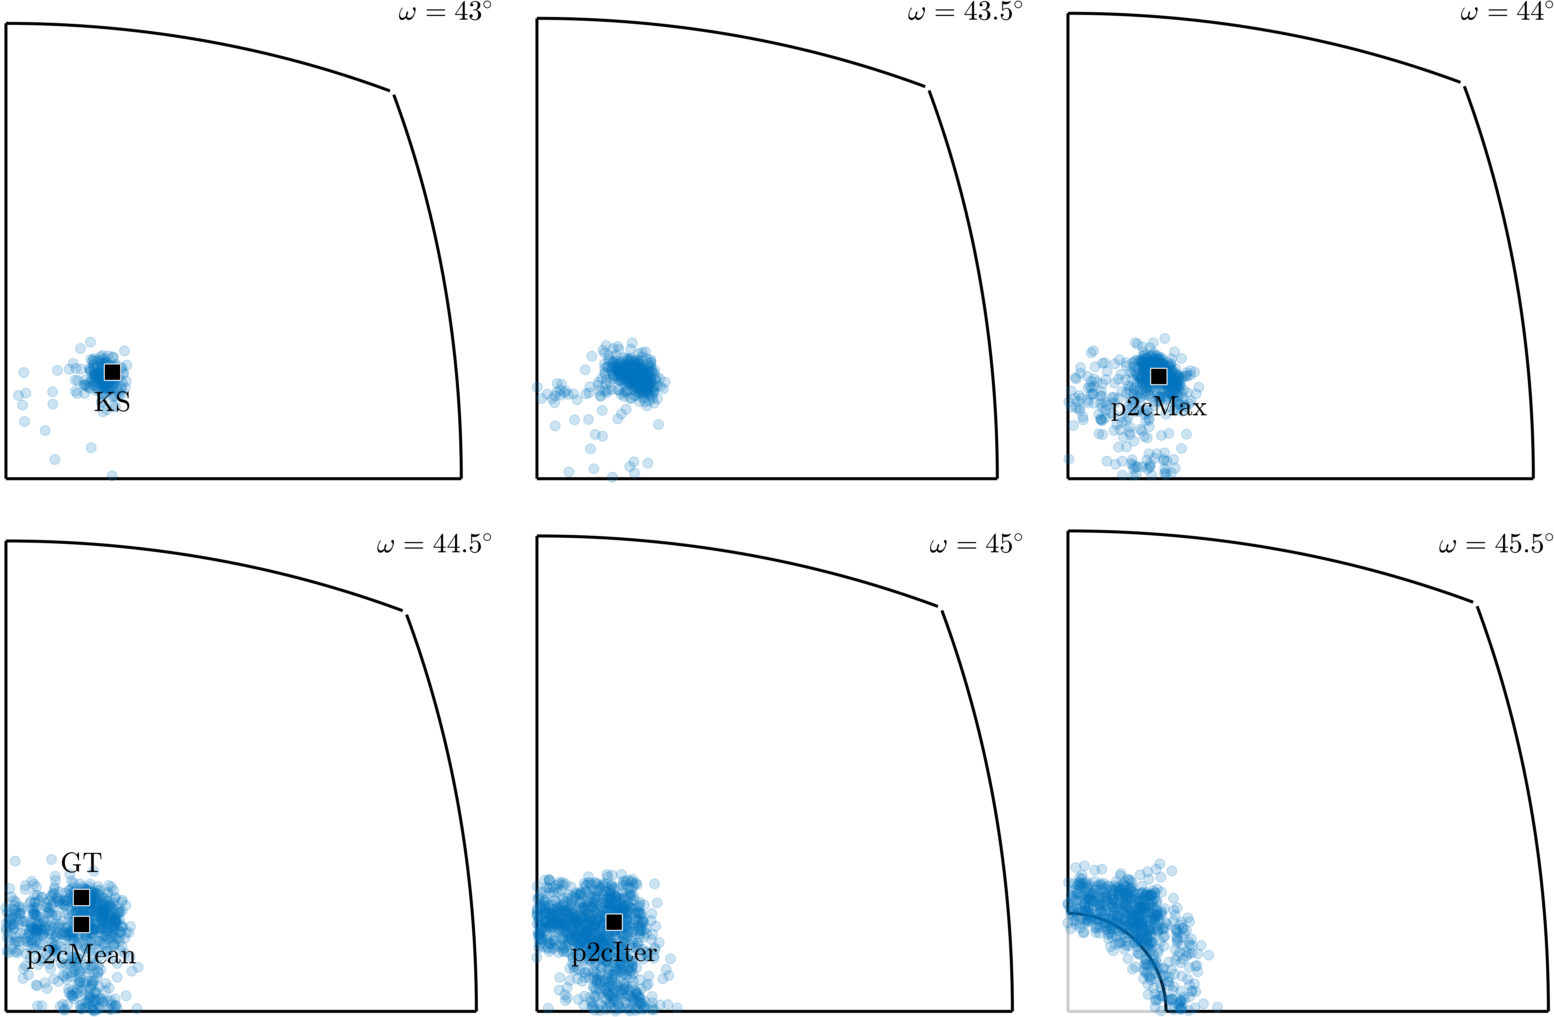
\includegraphics[width=0.8\textwidth]{pic/moriScatter}}
\end{center}


  \begin{overlayarea}{\textwidth}{3cm}
    \begin{itemize}
    \item<2-> Kurdjumov Sachs: $(111)_{\gamma} || (011)_{\alpha}$,
      $[\bar 101]_{\gamma}  || [\bar 1 \bar 1 1]_{\alpha}$
    \item<3-> NishiyamaWassermann: $(111)_{\gamma} || (011)_{\alpha}$,
      $[11\bar 2]_{\gamma}  || [0\bar 1 1]_{\alpha}$
    \item<4-> Greninger Trojano
    \end{itemize}

  \end{overlayarea}
\end{frame}


% \begin{frame}
%   \frametitle{The Parent to Child Orientation Relationship}

%   \begin{columns}
%     \begin{column}{0.55\textwidth}
%   \begin{block}{Notations}
%       \begin{itemize}
%       \item $\mathtt{ori_{P}}$ - parent orientation
%       \item $\mathtt{sym_{P}}$ - parent symmetry
%       \item $\mathtt{ori_{C}}$ - child orientation
%       \item $\mathtt{sym_{C}}$ - child symmetry
%     \item $\mathtt{p2c}$ - parent to child misorientation
%     \end{itemize}
%   \end{block}

%   \vspace{-0.5cm}

%       \begin{align*}
%         \mathtt{ori_{C}}
%         &= \mathtt{ori_{P}} \cdot \mathtt{sym_{P}} \cdot
%           \mathtt{inv}(\mathtt{p2c}) \cdot \mathtt{sym_{C}}\\
%         \mathtt{ori_{P}}
%         &= \mathtt{ori_{C}} \cdot \mathtt{sym_{C}} \cdot
%           \mathtt{p2c} \cdot \mathtt{sym_{P}}\\
%         \mathtt{p2c}
%         &= \mathtt{sym_{C}} \cdot \mathtt{inv}(\mathtt{ori_{C}}) \cdot
%           \mathtt{ori_{P}} \cdot \mathtt{sym_{P}}
%       \end{align*}

%       \begin{itemize}
%       \item $\mathtt{sym_{P}}$ describes the child variant
%       \item $\mathtt{sym_{C}}$ describes the parent variant
%       \end{itemize}
%     \end{column}
%     \begin{column}{0.4\textwidth}
%       \only<1>{
%         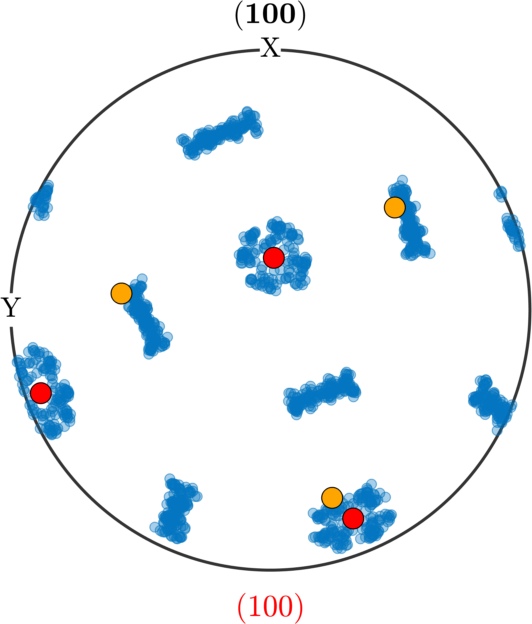
\includegraphics[width=\textwidth]{pic/pfSingleVariant1}}%
%       \only<2>{%
%         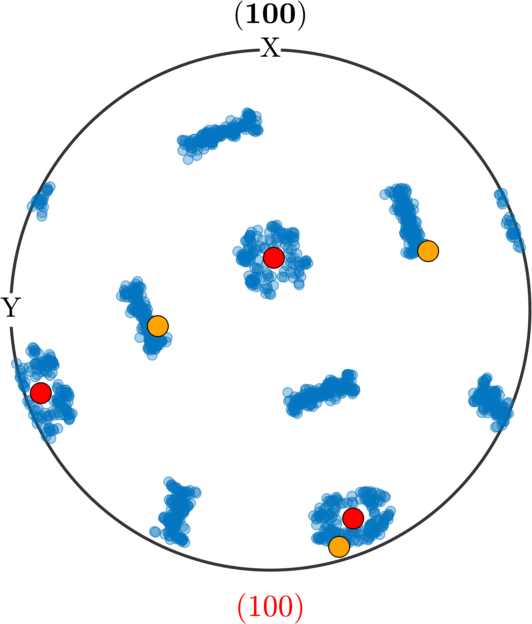
\includegraphics[width=\textwidth]{pic/pfSingleVariant2}}%
%       \only<3>{%
%         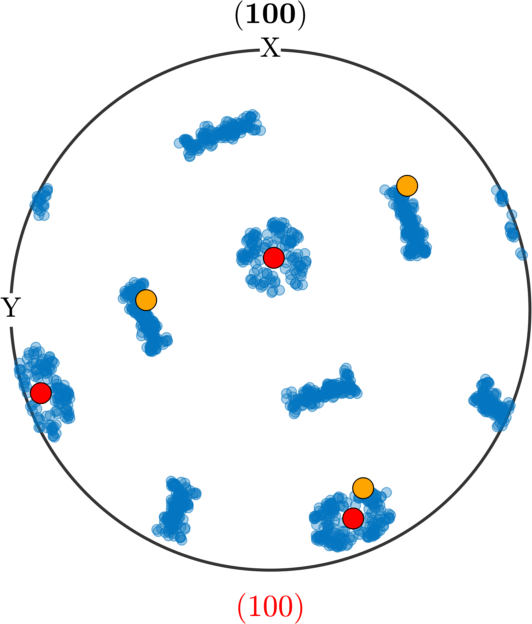
\includegraphics[width=\textwidth]{pic/pfSingleVariant3}}%
%       \only<4>{
%         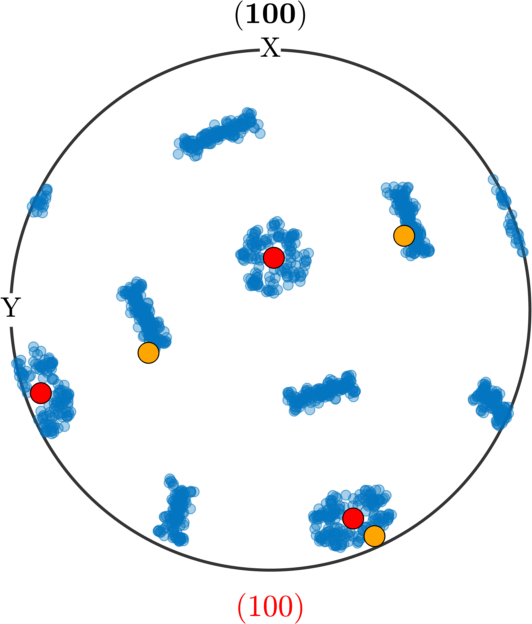
\includegraphics[width=\textwidth]{pic/pfSingleVariant4}}%
%       \only<5>{%
%         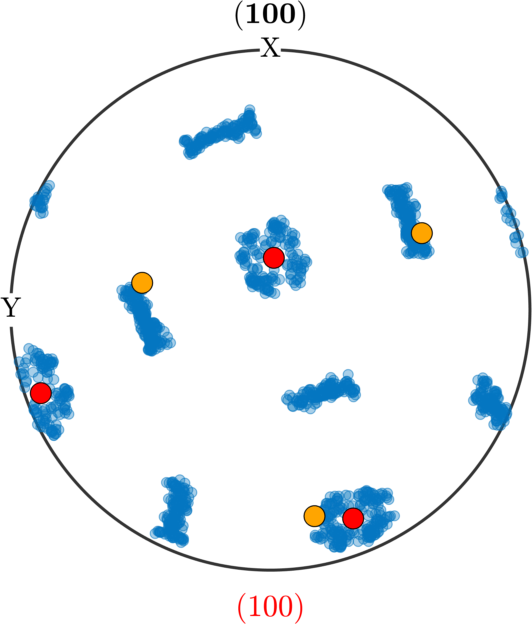
\includegraphics[width=\textwidth]{pic/pfSingleVariant5}}%
%       \only<6>{%
%         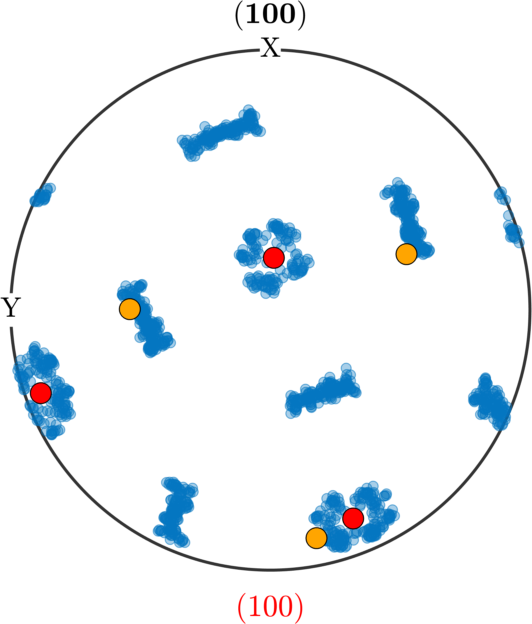
\includegraphics[width=\textwidth]{pic/pfSingleVariant6}}%
%       \only<7>{
%         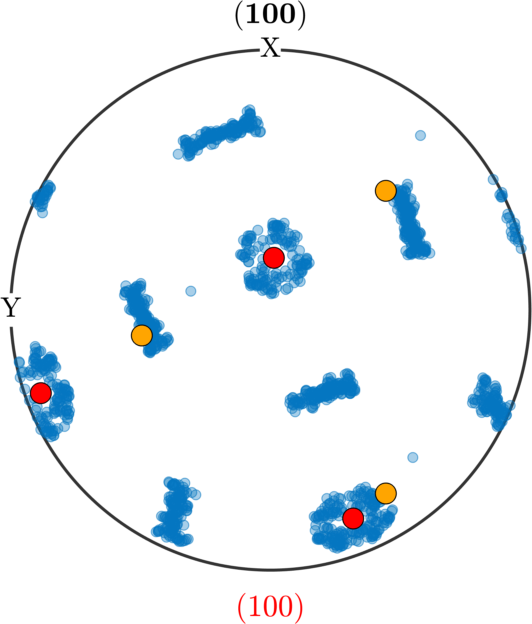
\includegraphics[width=\textwidth]{pic/pfSingleVariant7}}%
%       \only<8>{%
%         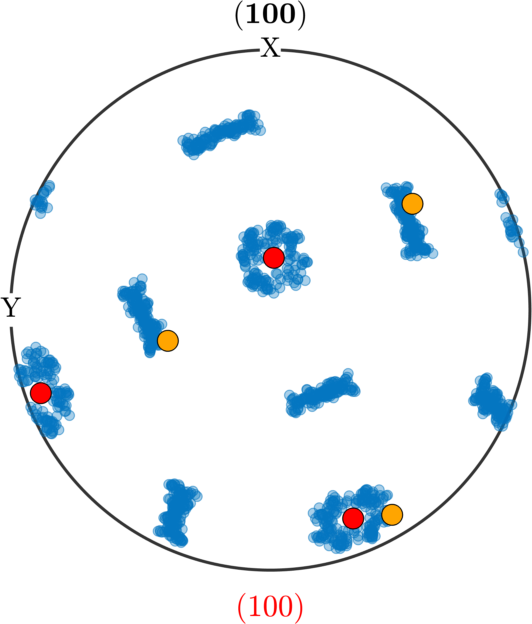
\includegraphics[width=\textwidth]{pic/pfSingleVariant8}}%
%       \only<9>{%
%         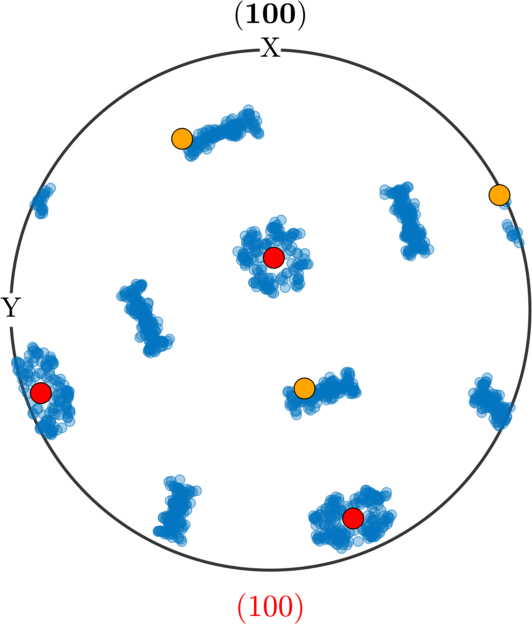
\includegraphics[width=\textwidth]{pic/pfSingleVariant9}}%
%       \only<10>{
%         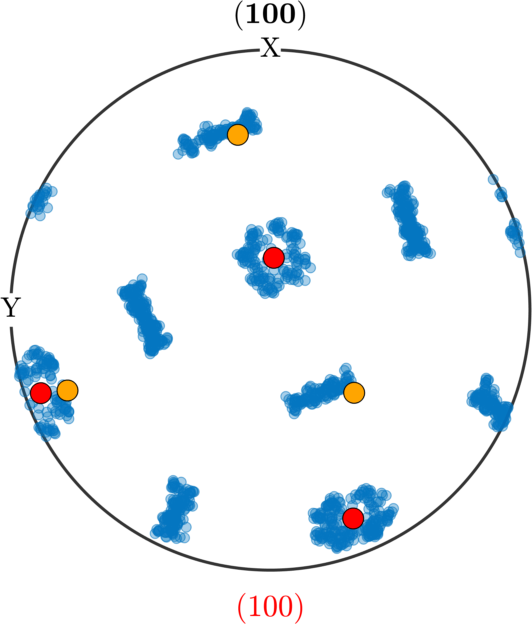
\includegraphics[width=\textwidth]{pic/pfSingleVariant10}}%
%       \only<11>{
%         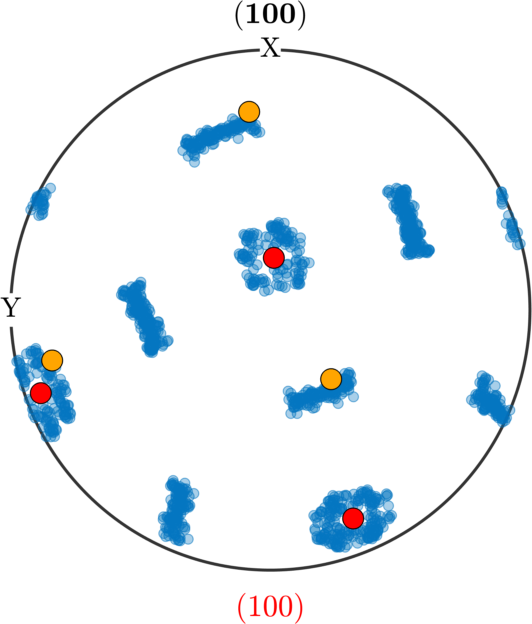
\includegraphics[width=\textwidth]{pic/pfSingleVariant11}}%
%       \only<12>{%
%         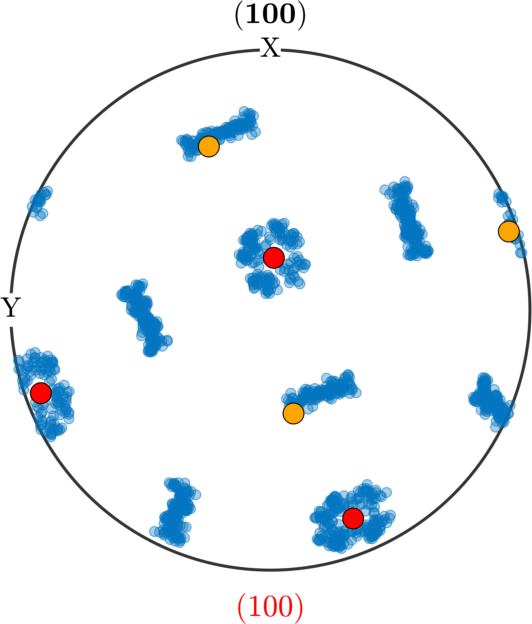
\includegraphics[width=\textwidth]{pic/pfSingleVariant12}}%
%       \only<13>{%
%         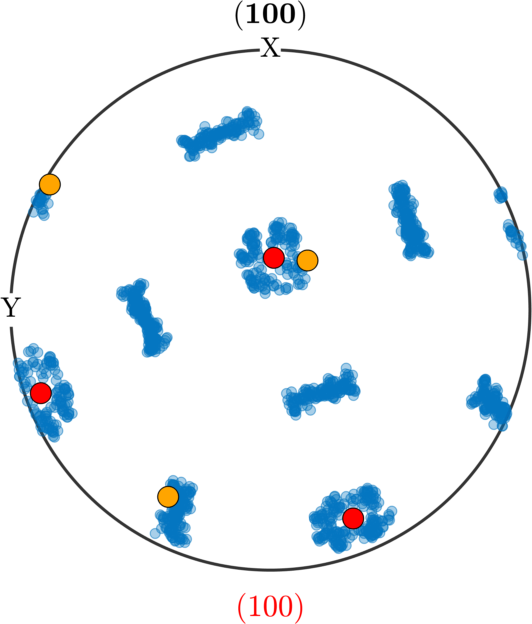
\includegraphics[width=\textwidth]{pic/pfSingleVariant13}}%
%       \only<14>{
%         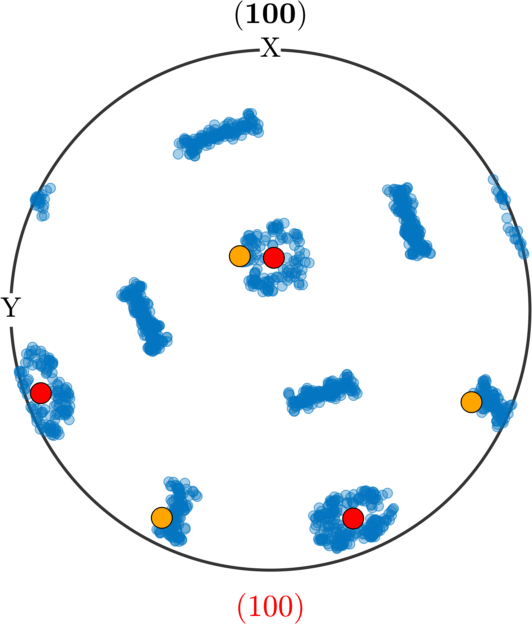
\includegraphics[width=\textwidth]{pic/pfSingleVariant14}}%
%       \only<15>{%
%         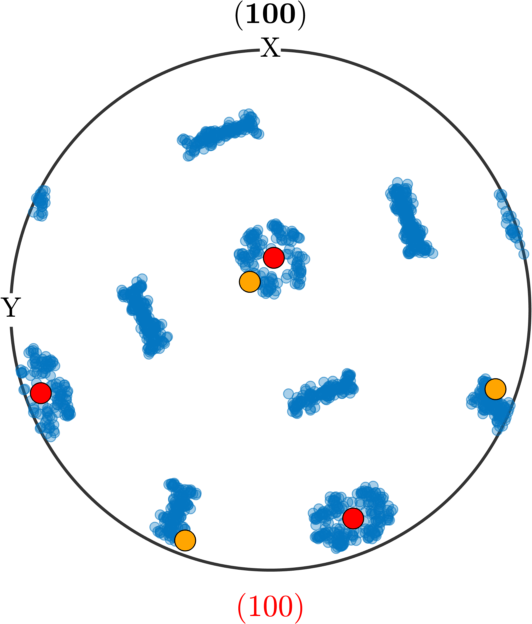
\includegraphics[width=\textwidth]{pic/pfSingleVariant15}}%
%       \only<16>{%
%         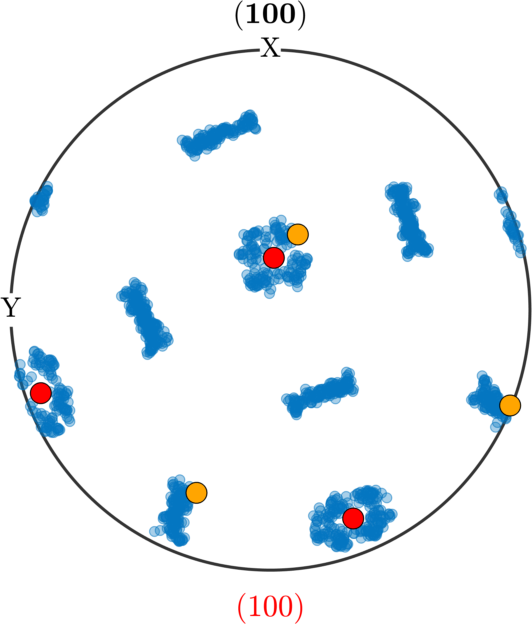
\includegraphics[width=\textwidth]{pic/pfSingleVariant16}}%
%       \only<17>{
%         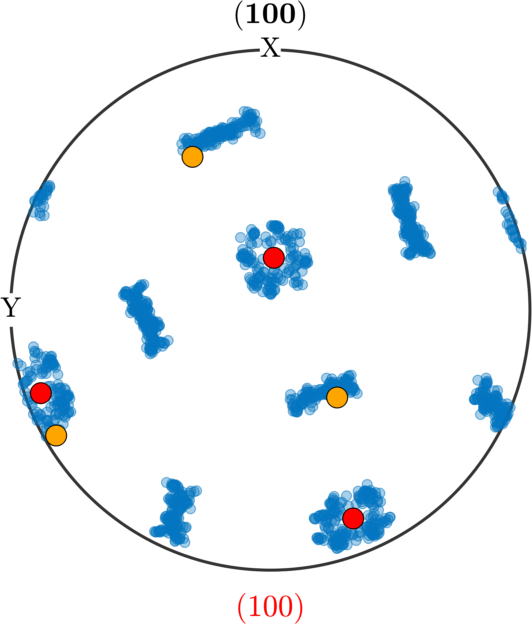
\includegraphics[width=\textwidth]{pic/pfSingleVariant17}}%
%       \only<18>{%
%         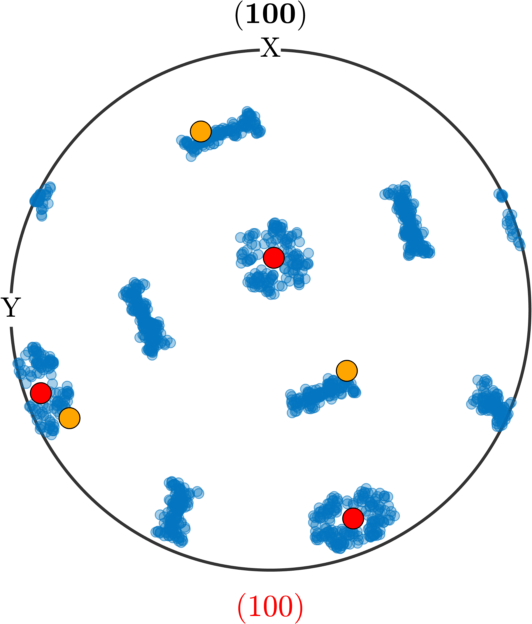
\includegraphics[width=\textwidth]{pic/pfSingleVariant18}}%
%       \only<19>{%
%         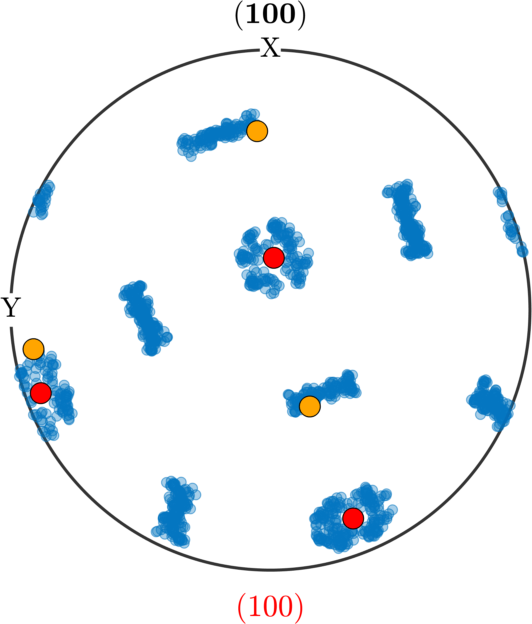
\includegraphics[width=\textwidth]{pic/pfSingleVariant19}}%

%     \end{column}
%   \end{columns}

% \end{frame}



\begin{frame}[fragile]
  \frametitle{Determining the ``True'' Orientation Relation Ship}

  \begin{center}
    \only<1>{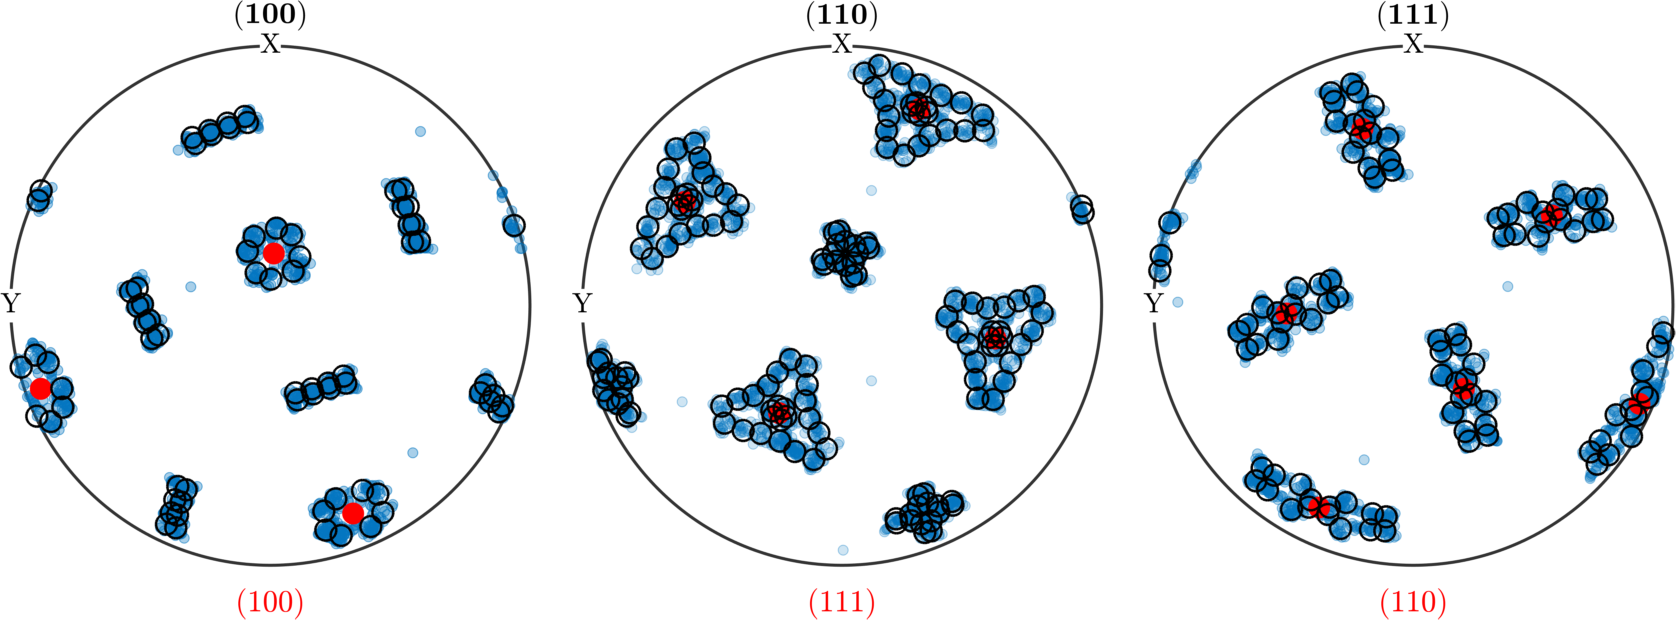
\includegraphics[width=0.95\textwidth]{pic/pfMean}}
    \only<2>{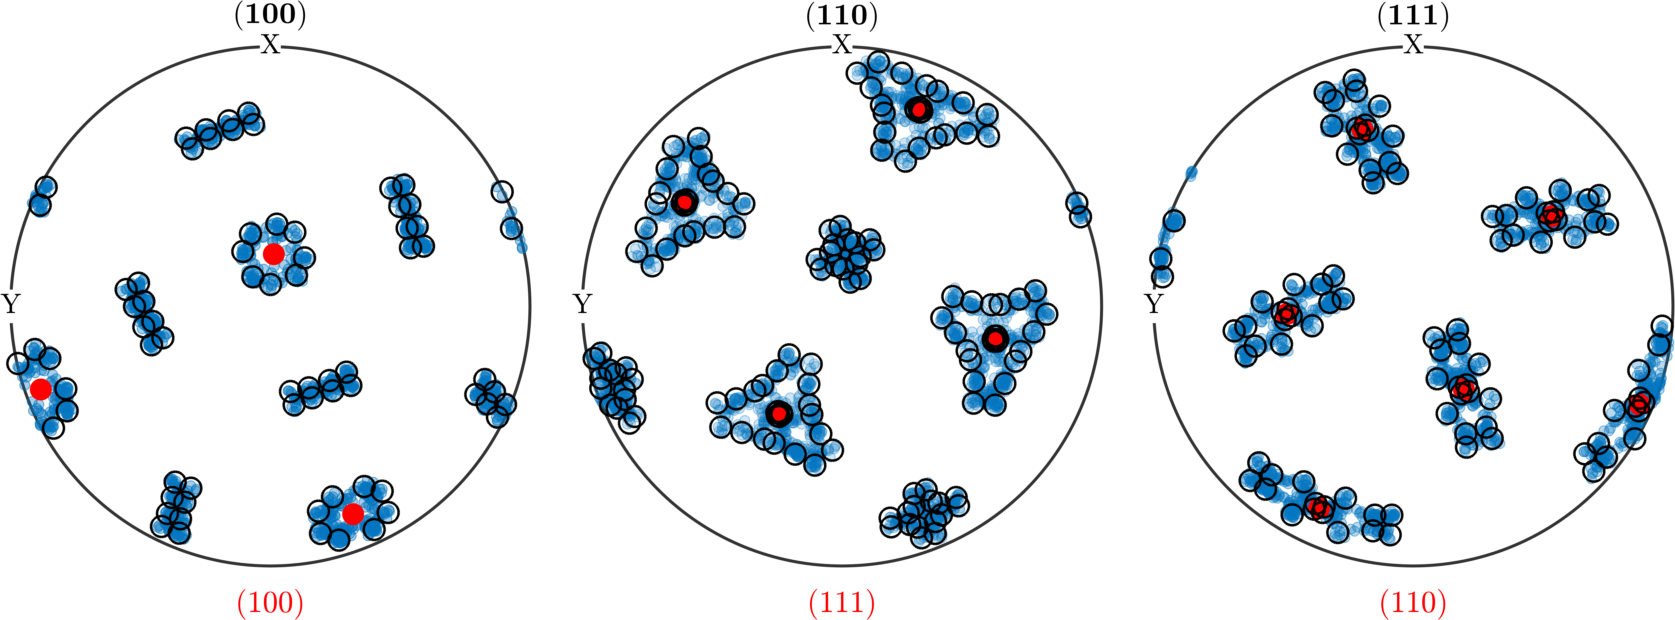
\includegraphics[width=0.95\textwidth]{pic/pfMax}}
    \only<3>{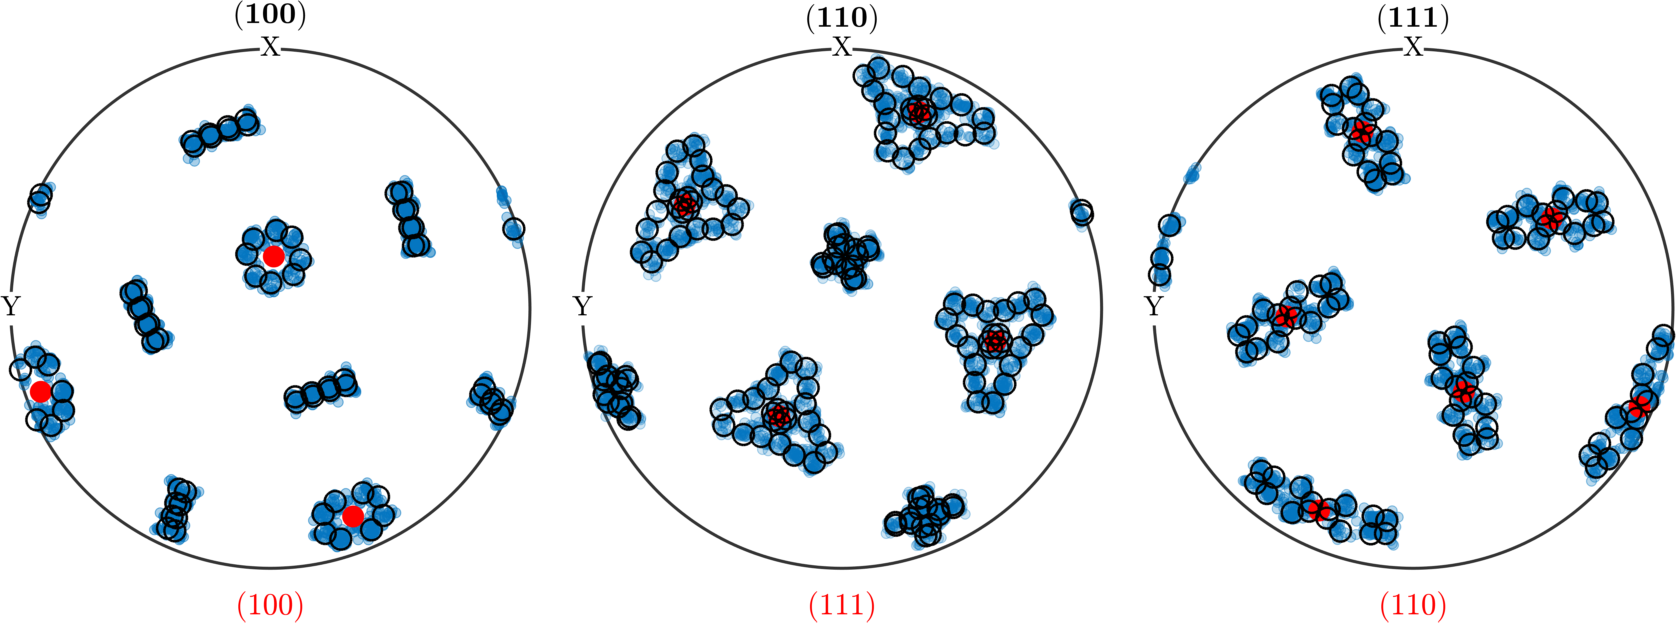
\includegraphics[width=0.95\textwidth]{pic/pfIter}}
    \only<4>{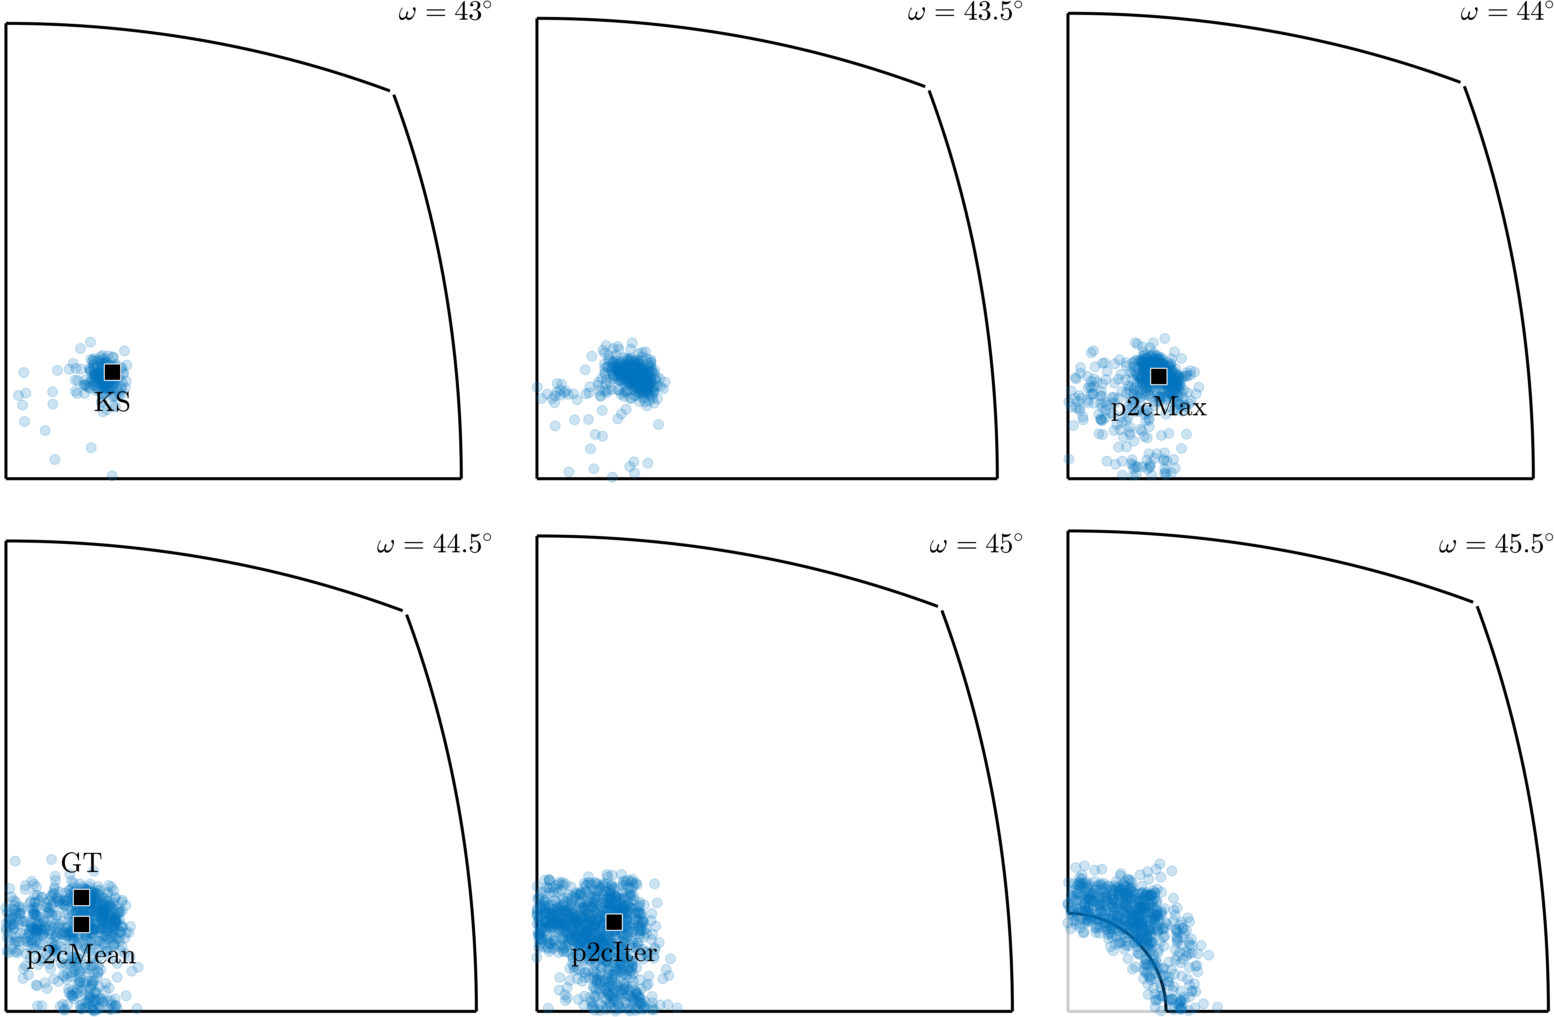
\includegraphics[width=0.85\textwidth]{pic/moriScatter.png}}
  \end{center}
  \begin{overlayarea}{\textwidth}{3cm}
    \begin{itemize}
    \item<1-3> average parent to child misorientation%: \lstinline{p2cMean = mean( inv(oriChild) * oriP )}
    \item<2-3> maximum of misorientation distribution function
      \uncover<4>{\paritem iterative method of T. Nyyssönen}
    \end{itemize}
  \end{overlayarea}

% % \begin{lstlisting}[style=input]
% % p2cMean = mean( inv(oriChild) * oriP)
% % \end{lstlisting}
%   \item take the maximum of the misorientation distribution function
%     \begin{lstlisting}[style=input]
% mdf = calcDensity( inv(oriChild) * oriP)
% [value,p2cMax] = max(mdf)
% \end{lstlisting}

\end{frame}


%\section{Variant Detection}

\section{Identifying Child to Child Neighborships}

\begin{frame}[fragile]
  \frametitle{Identifying Child to Child Neighborships}


  \begin{columns}
    \begin{column}{0.7\textwidth}
      \begin{overlayarea}{\textwidth}{0.8\textheight}
      \only<1>{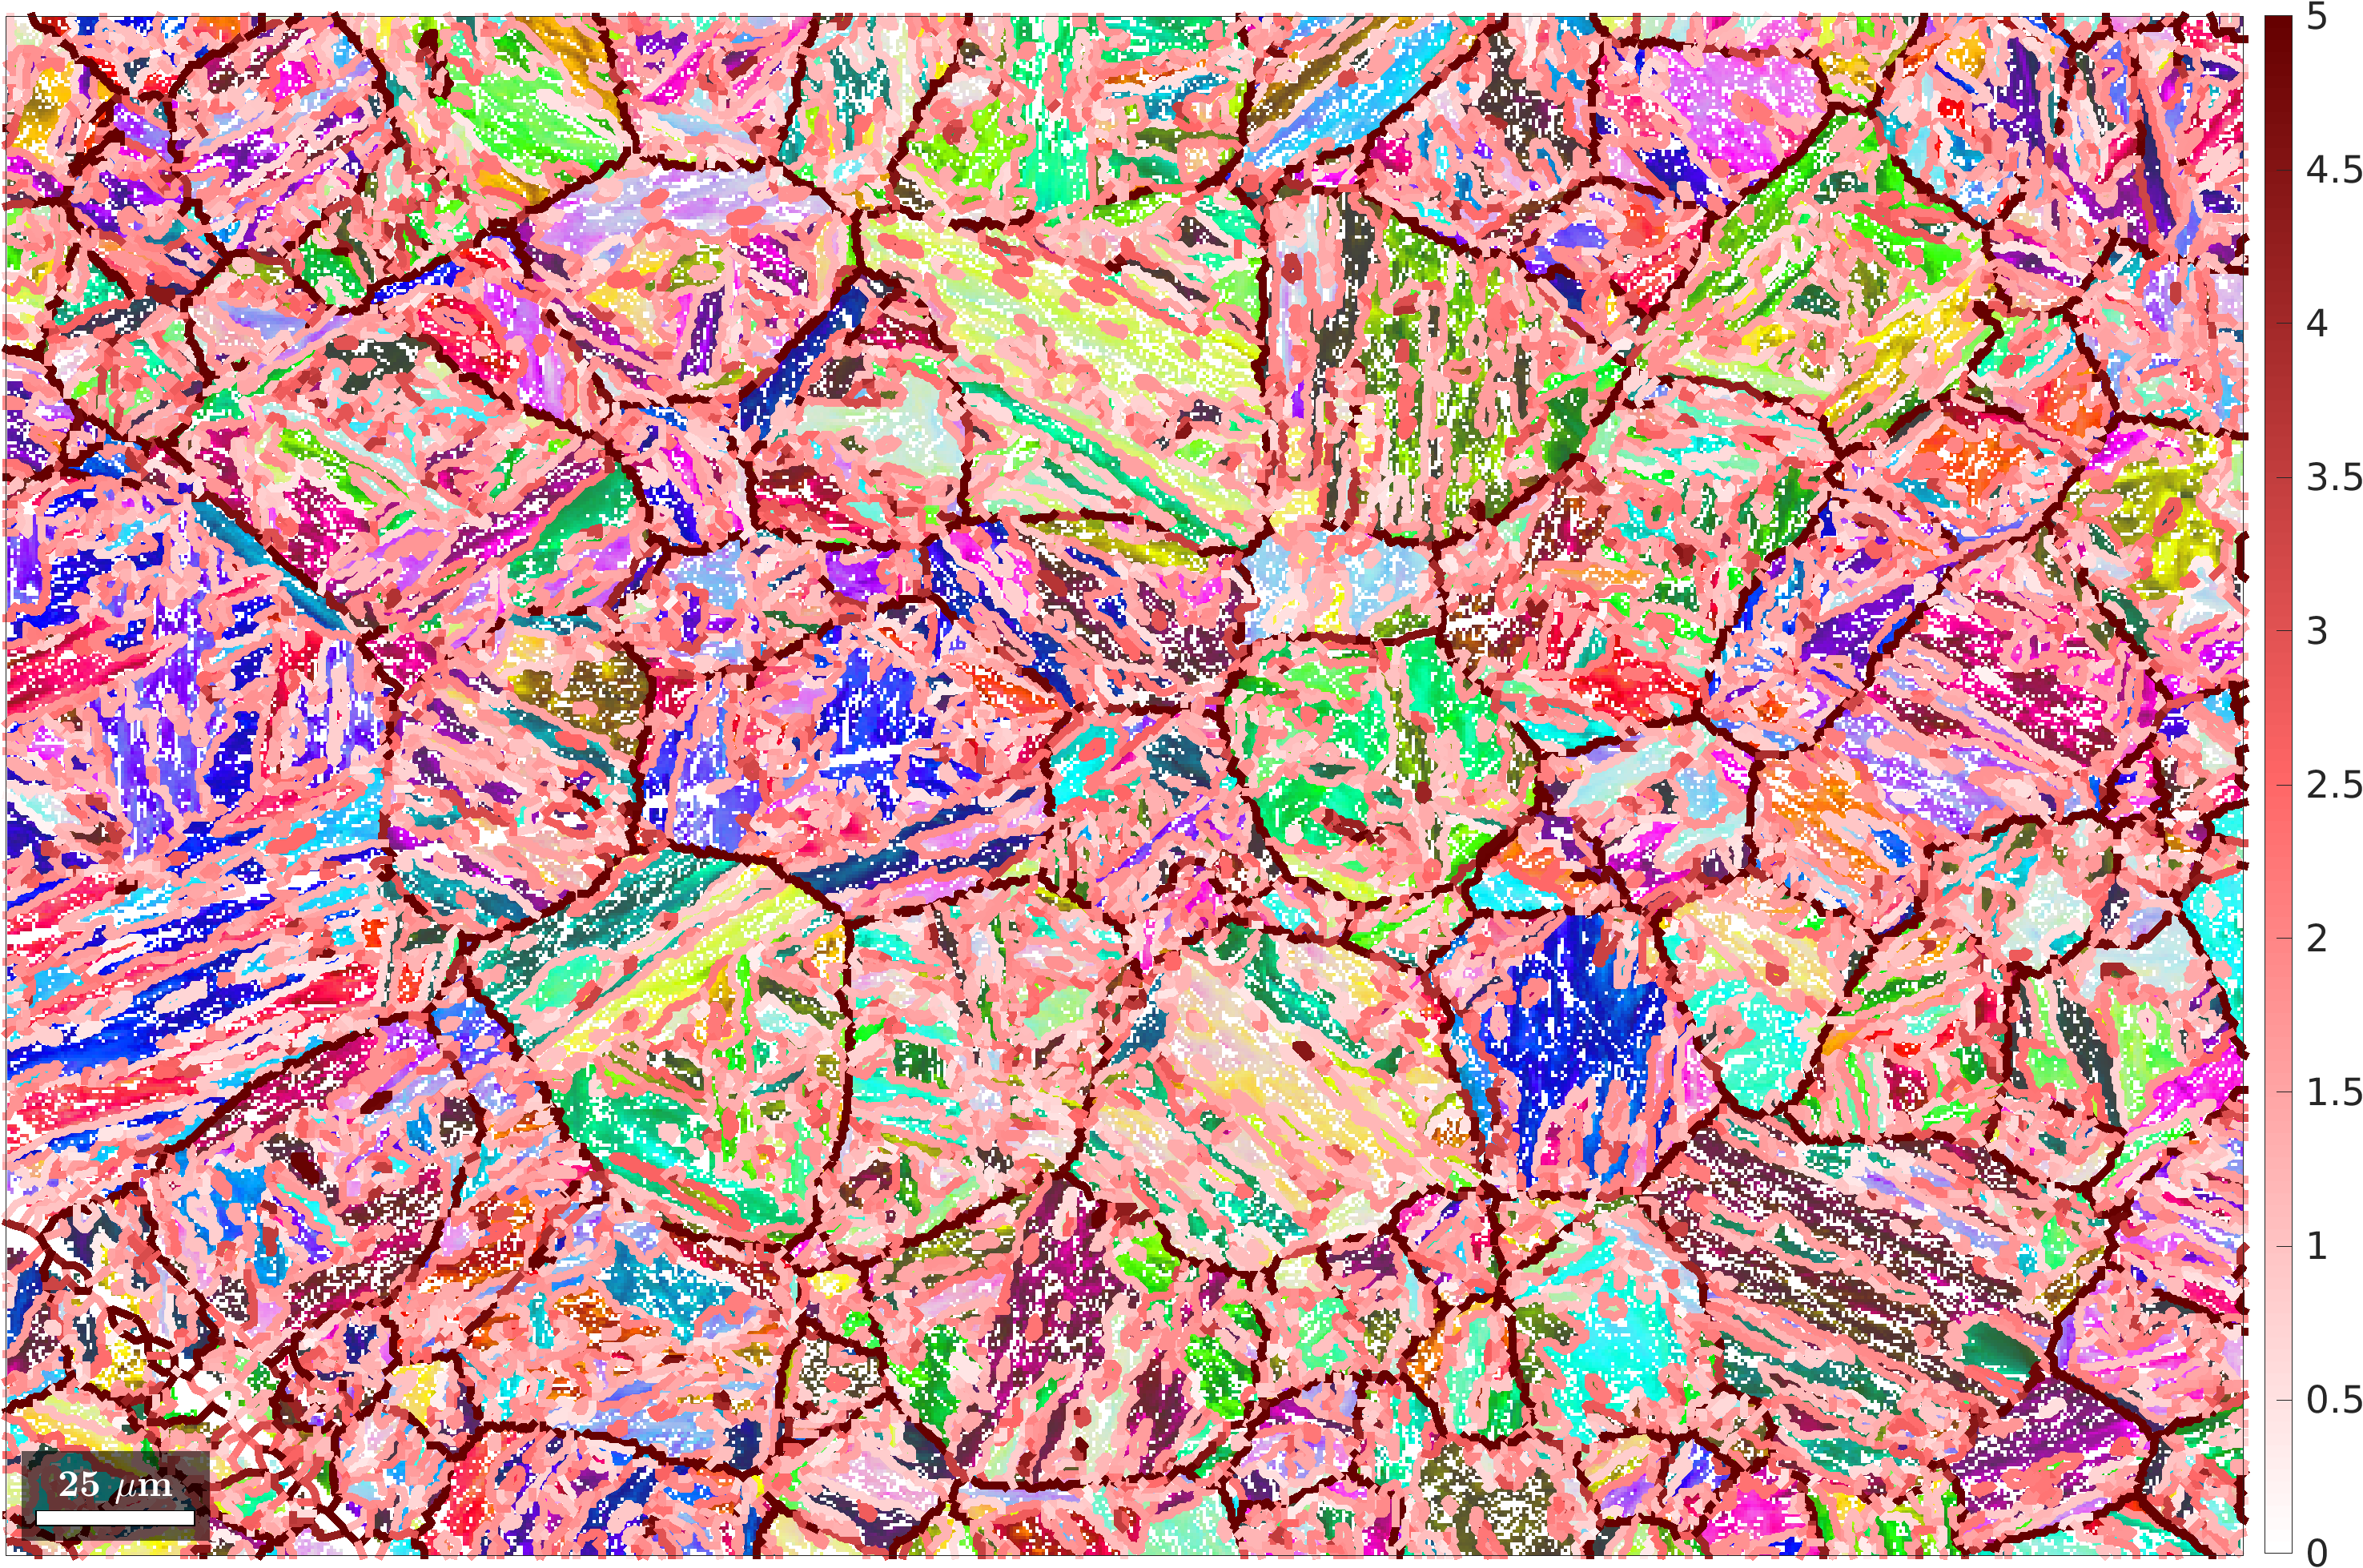
\includegraphics[width=\textwidth]{pic/gBFit}}
      \only<2>{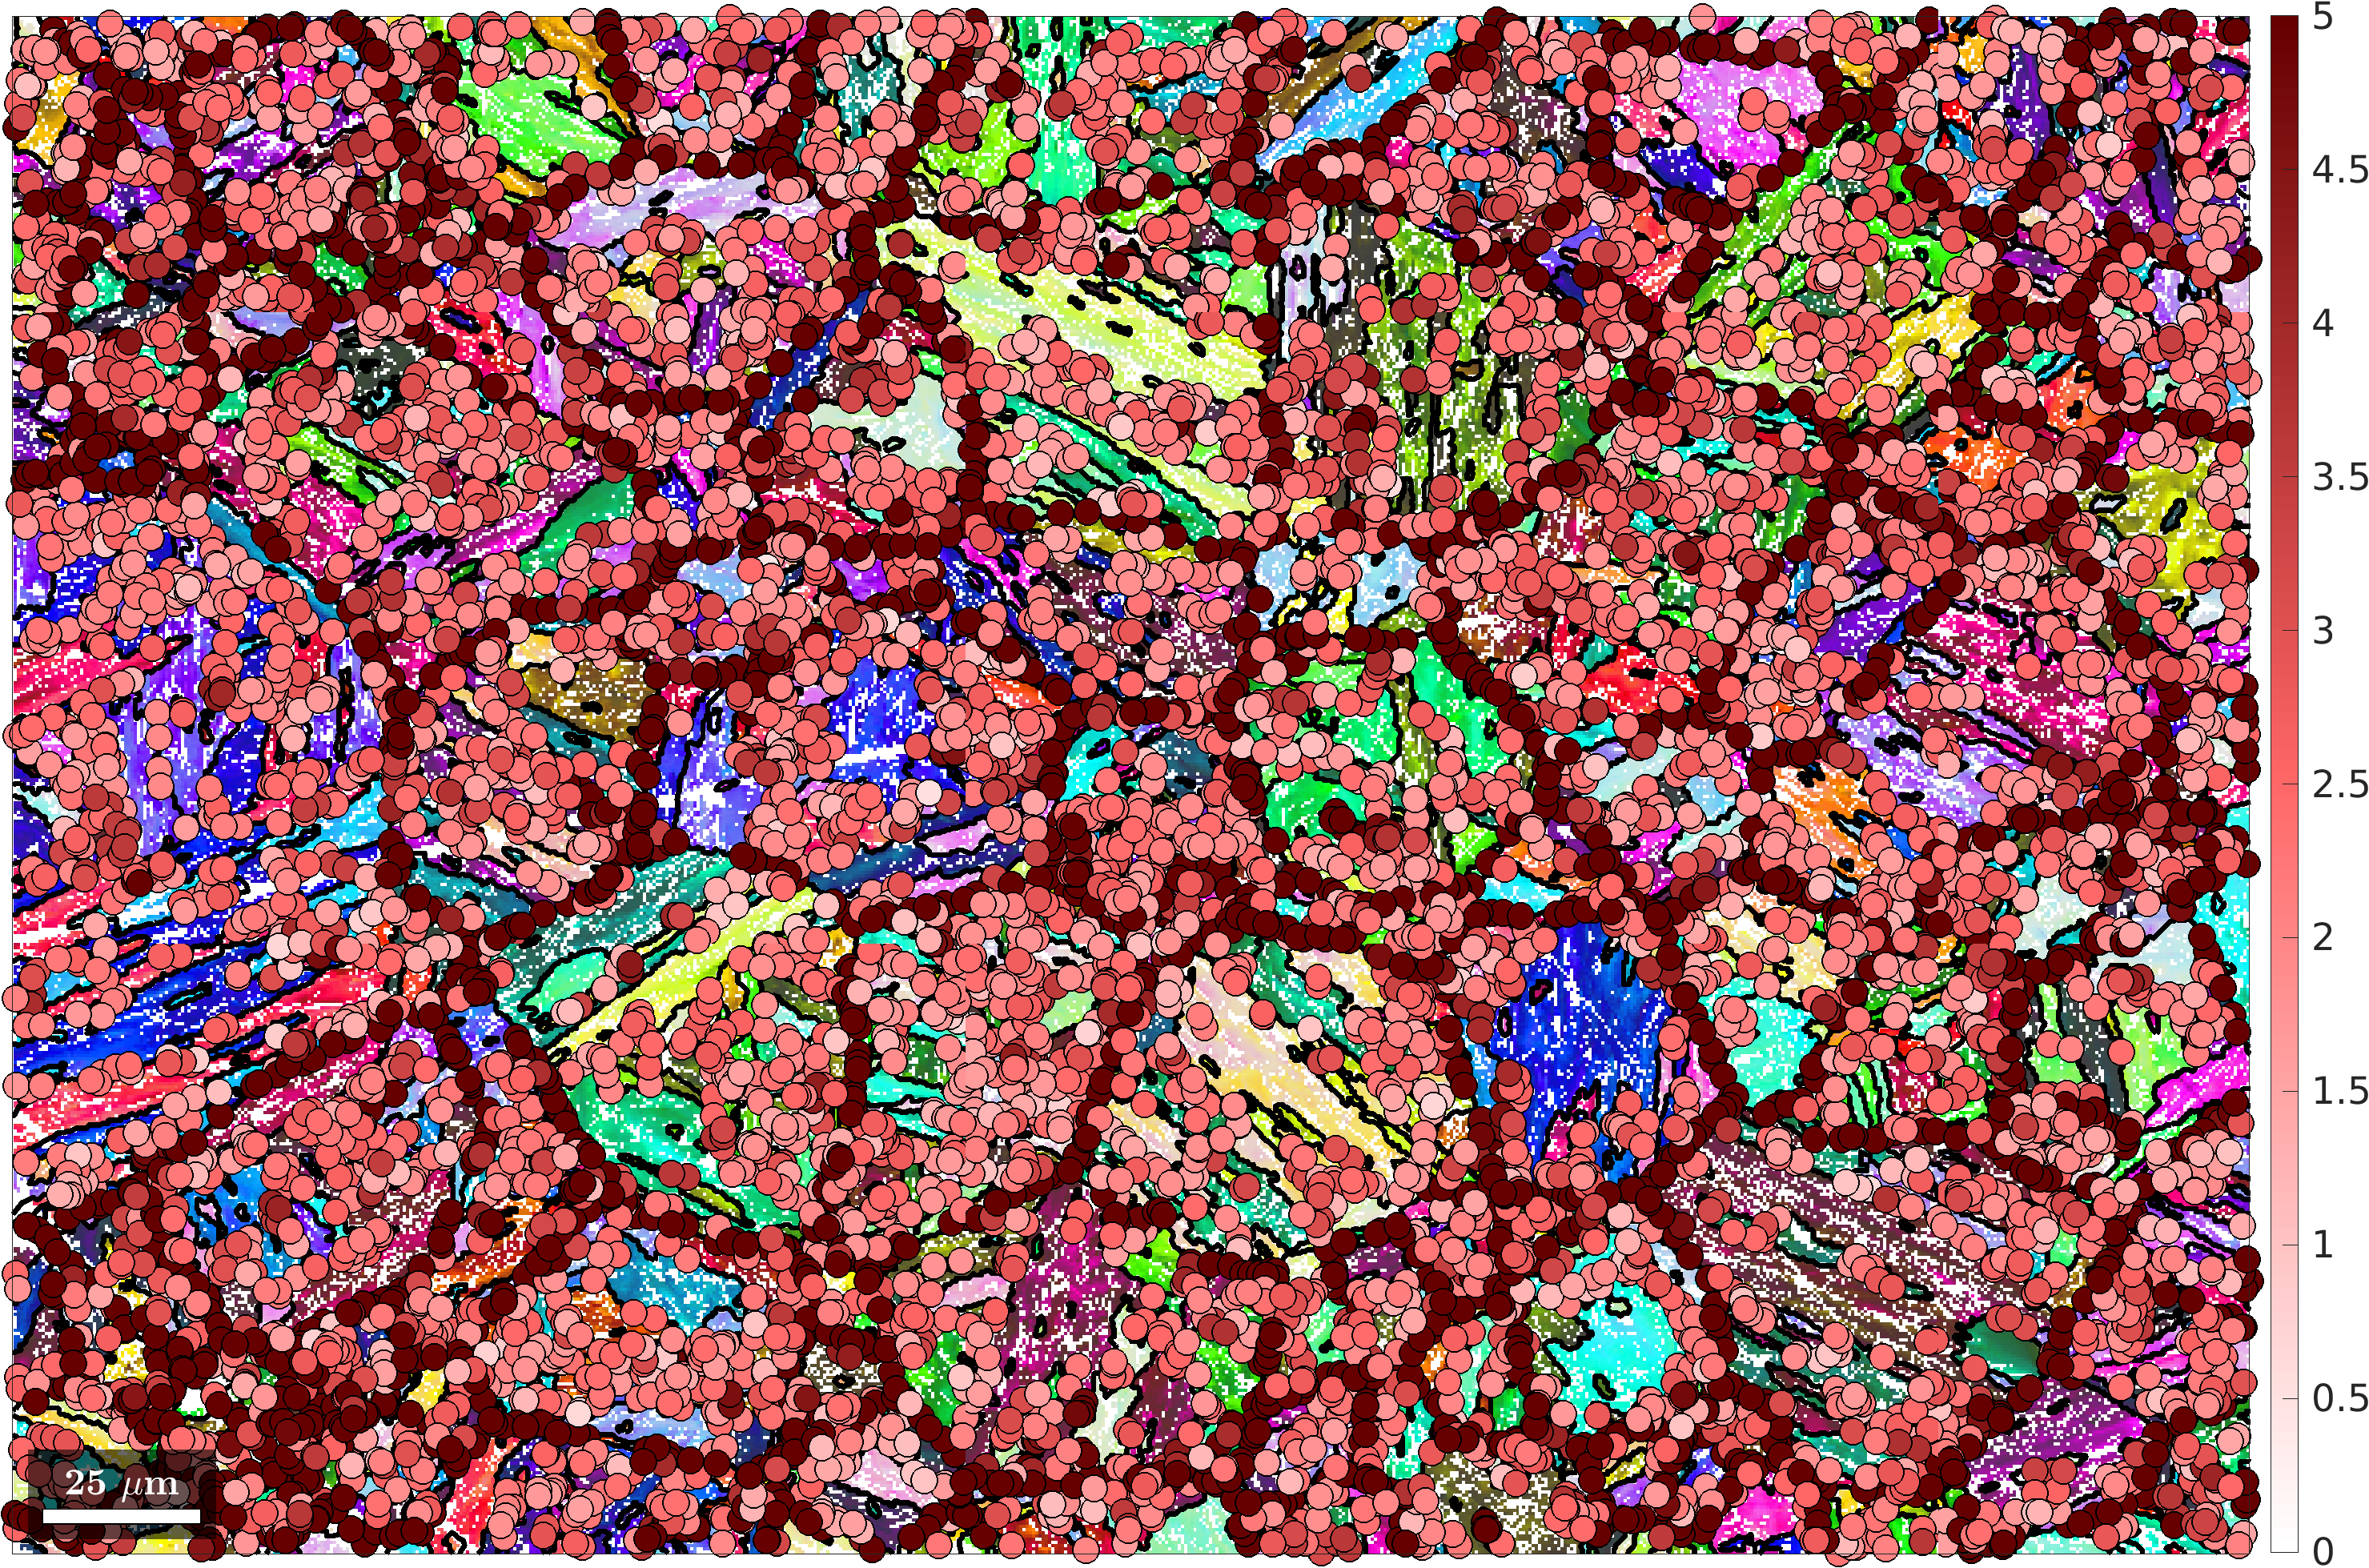
\includegraphics[width=\textwidth]{pic/tPFit}}
    \end{overlayarea}
  \end{column}
    \begin{column}{0.28\textwidth}
      \begin{overlayarea}{\textwidth}{0.8\textheight}
        \only<1->{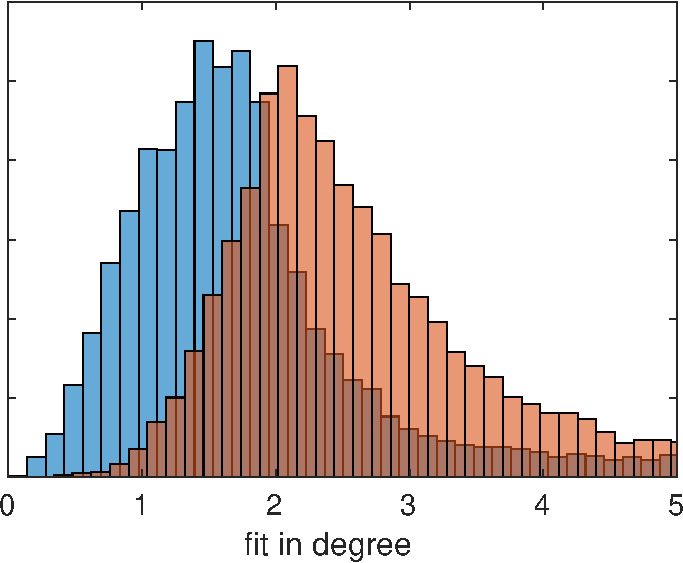
\includegraphics[width=1\textwidth]{pic/histGB}}
        \only<2>{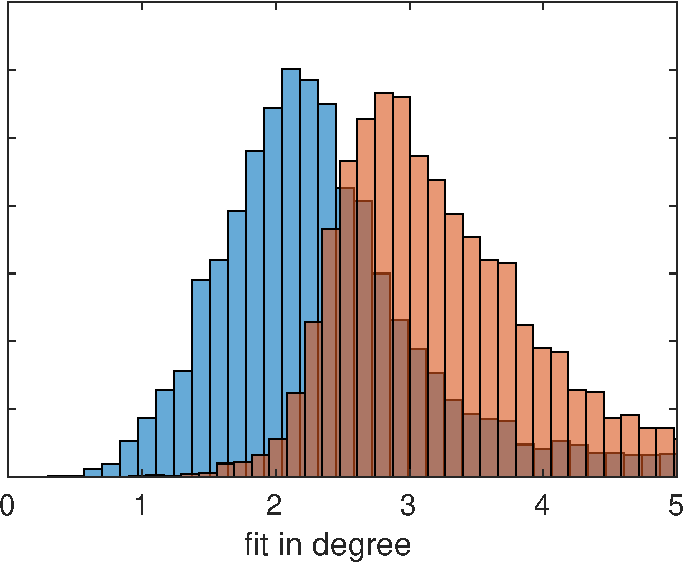
\includegraphics[width=1\textwidth]{pic/histTP}}
      \end{overlayarea}
    \end{column}
  \end{columns}


% \begin{lstlisting}[style=input]
% [parentId, fit] = calcParent(gBori,p2c,'numFit',2,'id');
% \end{lstlisting}

  % \begin{equation*}
  %   \mathtt{fit}
  %   = \min \angle(\mathtt{c2c}, \mathtt{p2c} \cdot \mathtt{sym_{p}}
  %   \cdot \mathtt{inv}(\mathtt{p2c}))
  % \end{equation*}

\end{frame}

% \begin{frame}[fragile,fragile]
%   \frametitle{Identifying Child to Child Orientation Relationships at Triple
%     Junctions}

%   \begin{center}

%   \end{center}

% \begin{lstlisting}[style=input]
% [parentId, fit] = calcParent(tPori,p2c,'numFit',2,'id');
% \end{lstlisting}

% \end{frame}


\section{Parent Grain Reconstruction}

\begin{frame}[fragile]
  \frametitle{Parent Grain Reconstruction}
  \begin{columns}%
    \begin{column}{0.475\textwidth}%
      \begin{overlayarea}{\textwidth}{0.95\textheight}%
        \vspace{-0.3cm}
        \begin{block}{orientation first - grain second}
          \begin{enumerate}
          \item<2-> for each child grain\\
            \hspace{-0.8cm}\paritem collect votes for the parent orientation\\
            \hspace{-0.8cm}\paritem majority vote decides parent orientation\\
            \hspace{-0.8cm}\paritem turn child into parent grains
          \item<3-> merge parent grains by orientation
          \item<4-> merge child to parent grains
          \end{enumerate}
        \end{block}

        \begin{block}{grain first - orientation second}
          \begin{enumerate}
          \item<6-> define weighted child graph
          \item<7-> weight is fit to reference \texttt{c2c}
          \item<8-> cut graph into clusters
          \item<9-> clusters are parent grains
          \item<10-> compute parent orientations
          \item<11-> merge parent grains by orientation
          \end{enumerate}
        \end{block}
      \end{overlayarea}
    \end{column}
    \begin{column}{0.45\textwidth}
      \begin{overlayarea}{\textwidth}{0.9\textheight}
        \only<1>{\vspace{-1cm}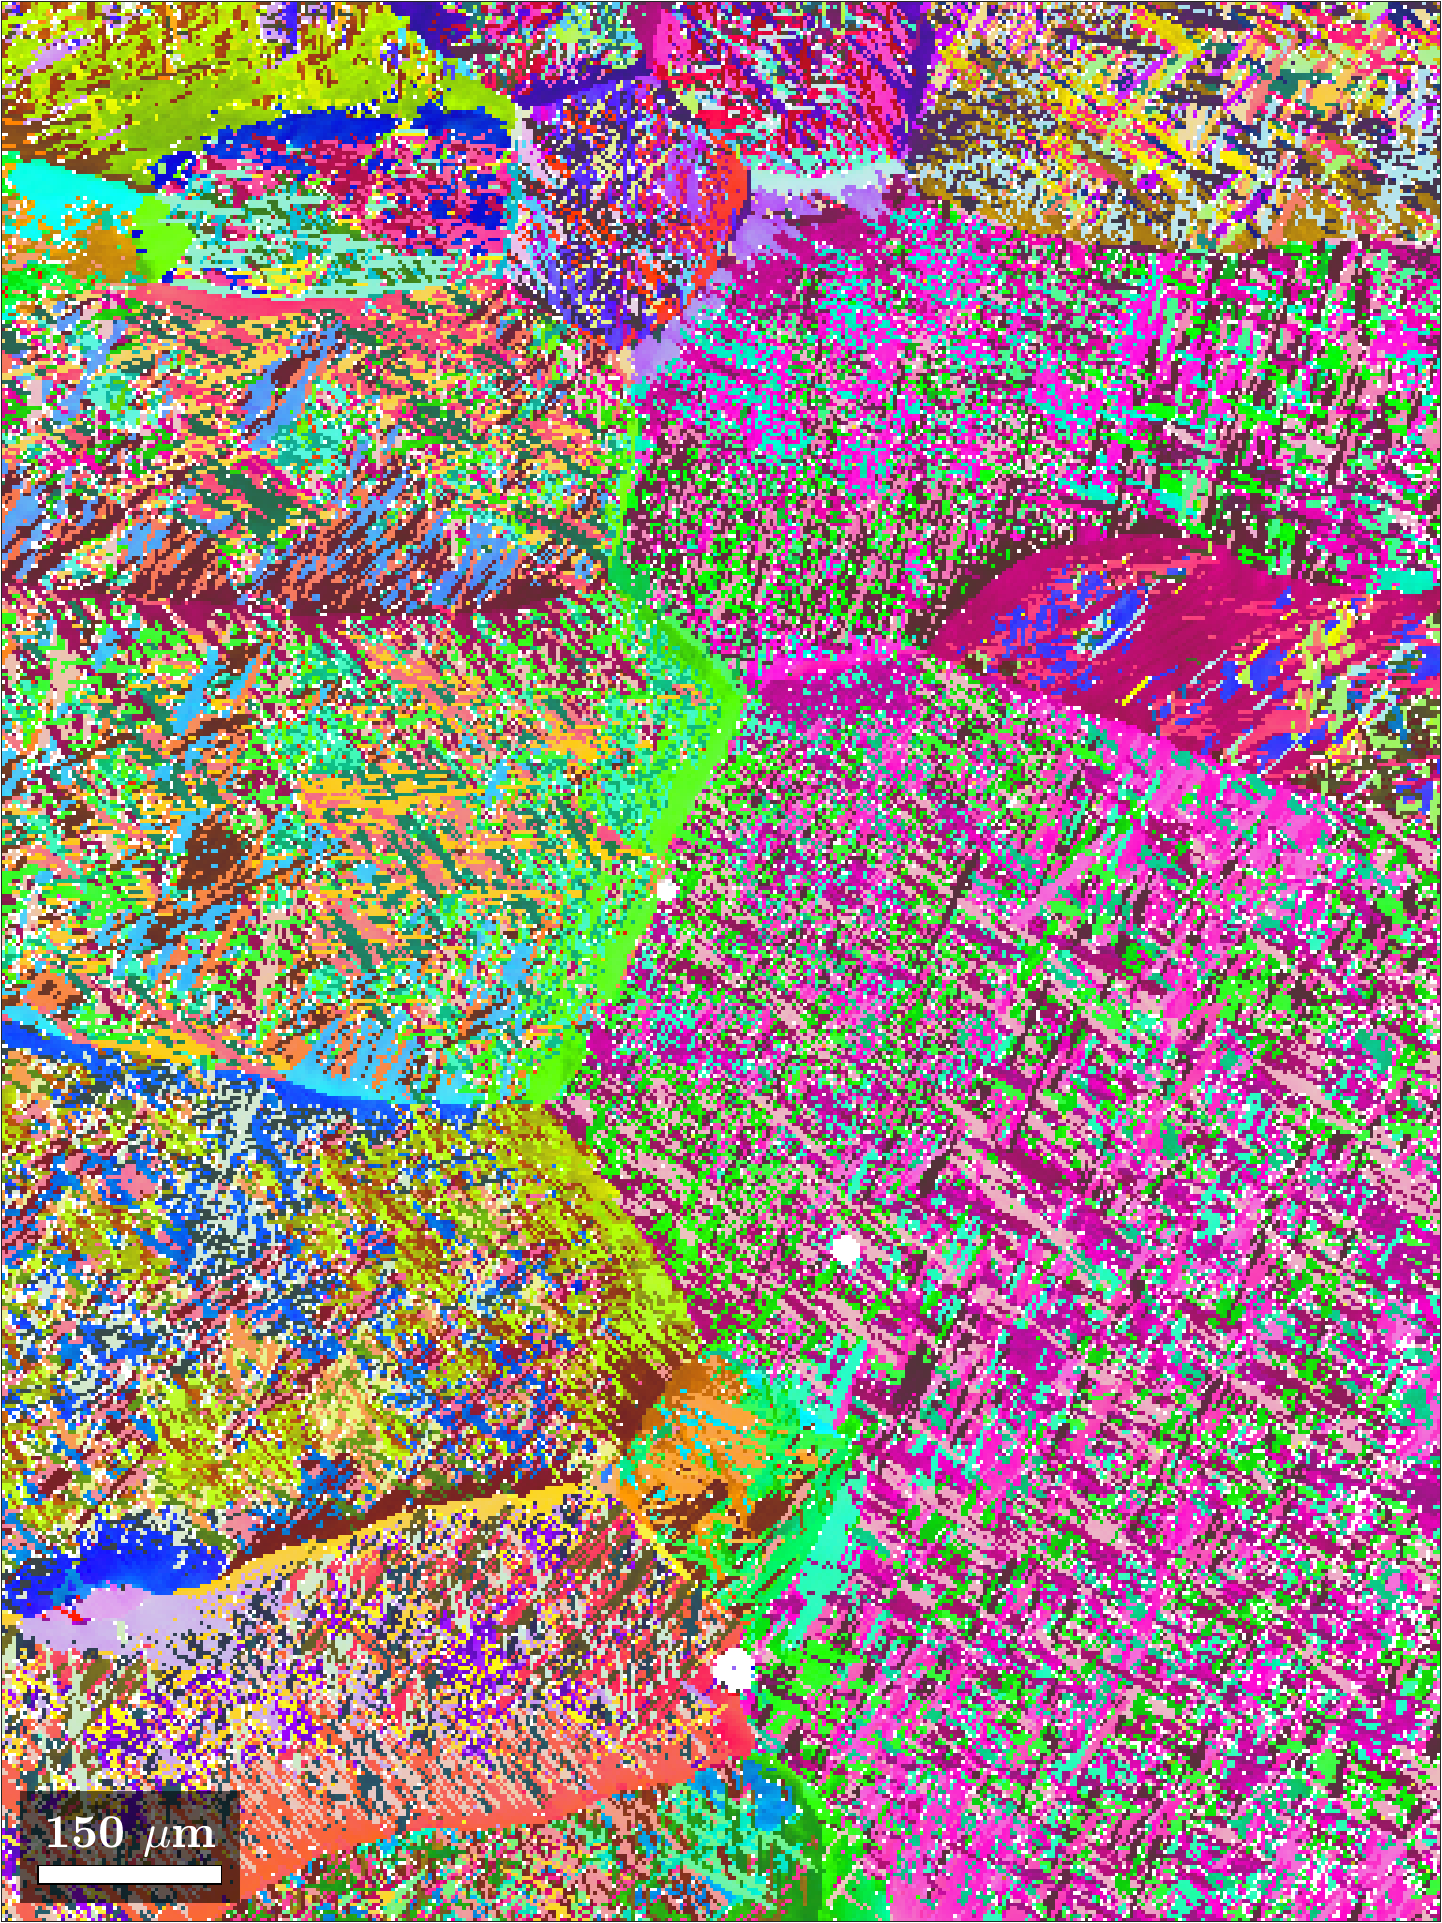
\includegraphics[width=\textwidth]{pic/TiMap}}
        \only<2>{\vspace{-1cm}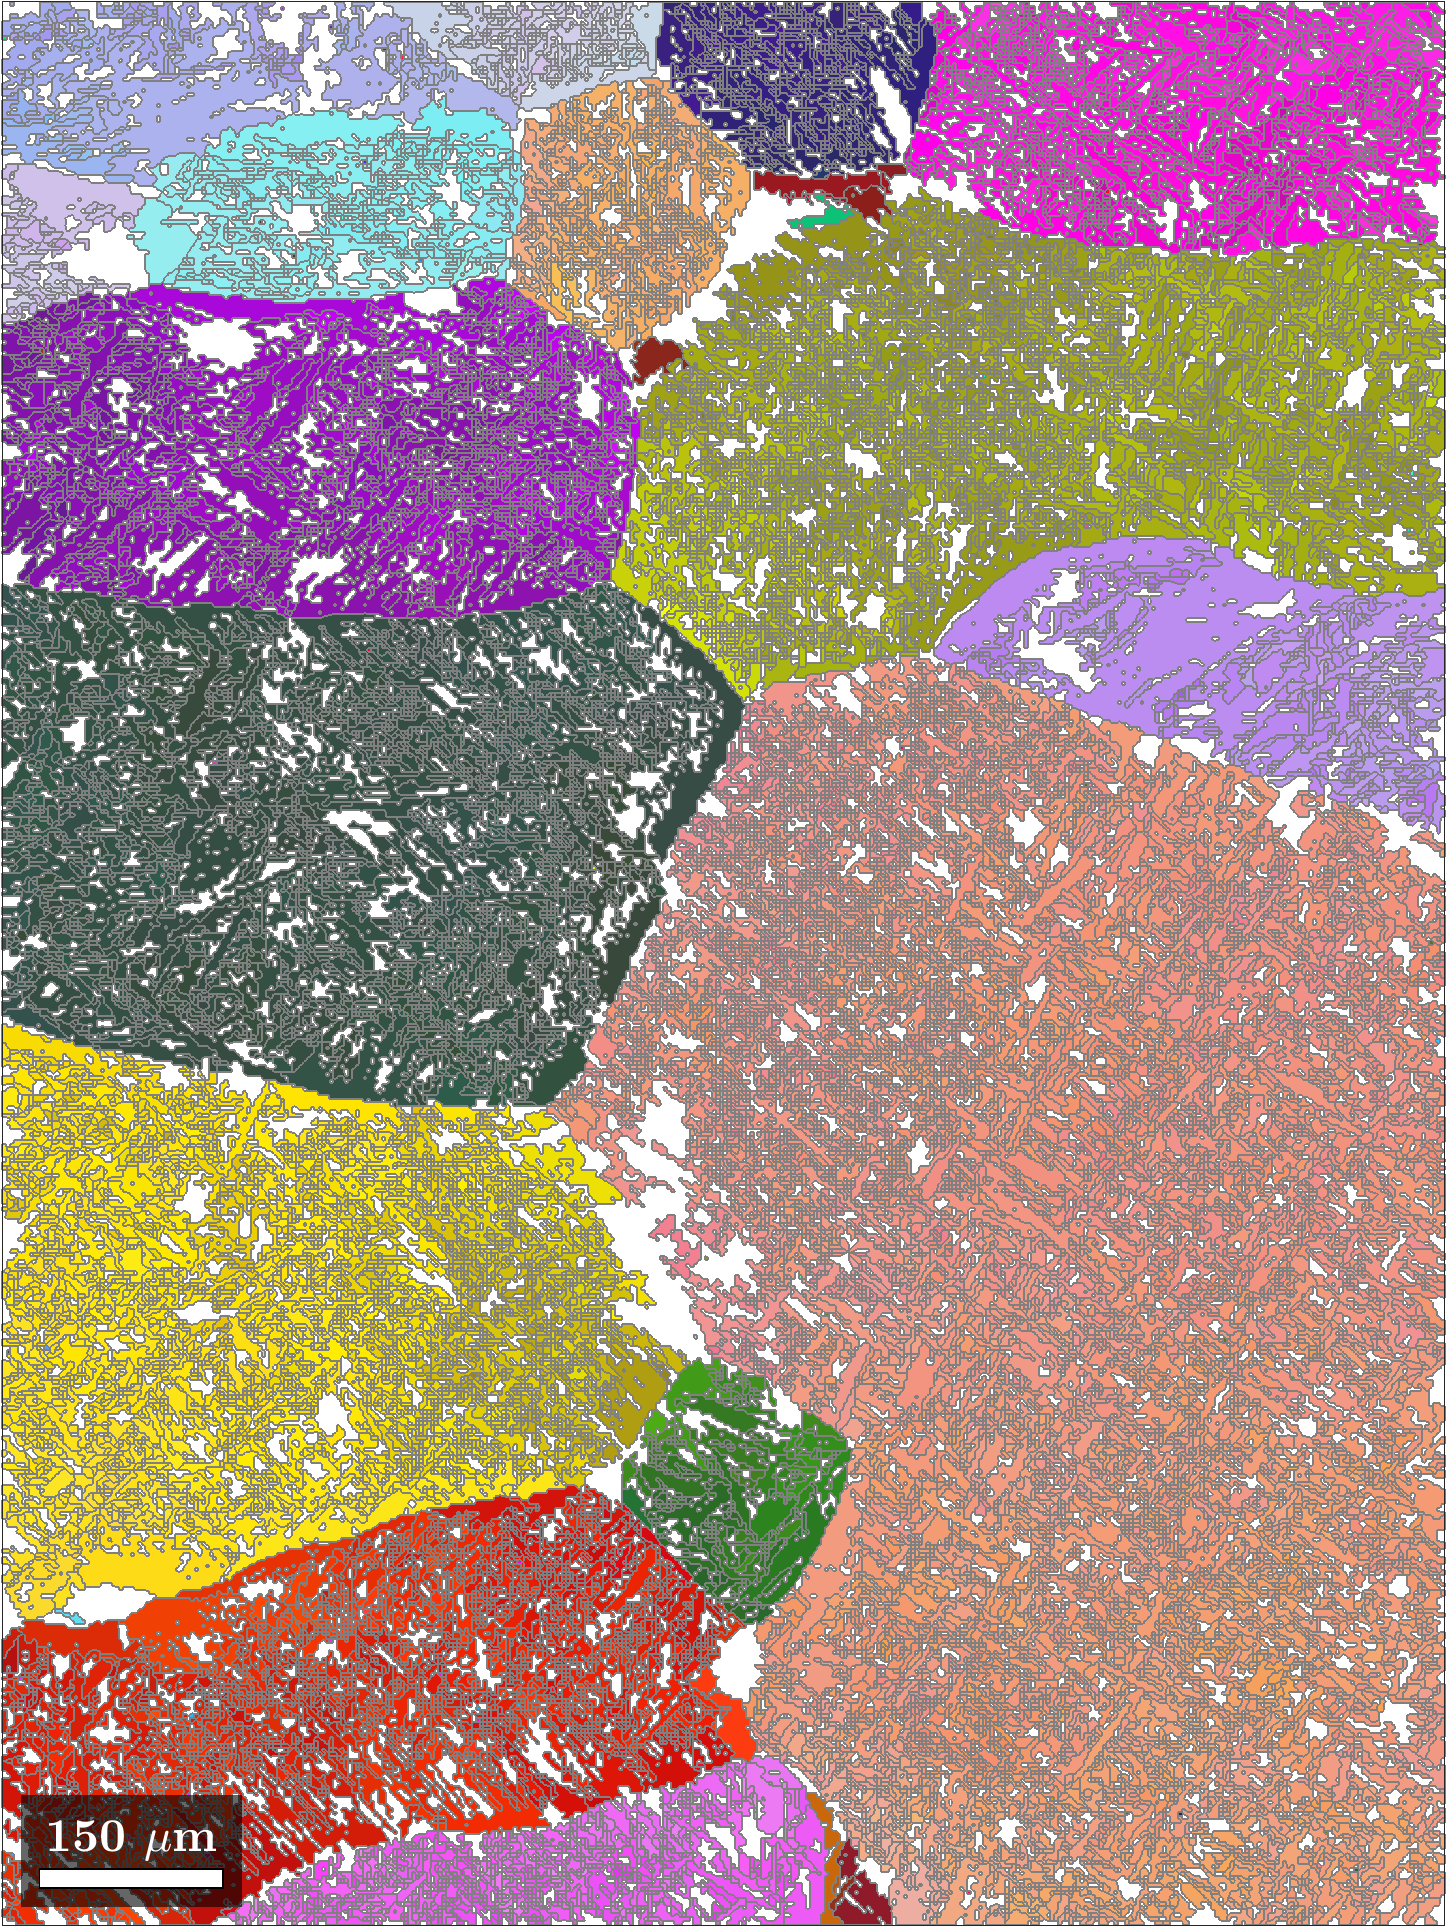
\includegraphics[width=\textwidth]{pic/TiParentOri}}
        \only<3>{\vspace{-1cm}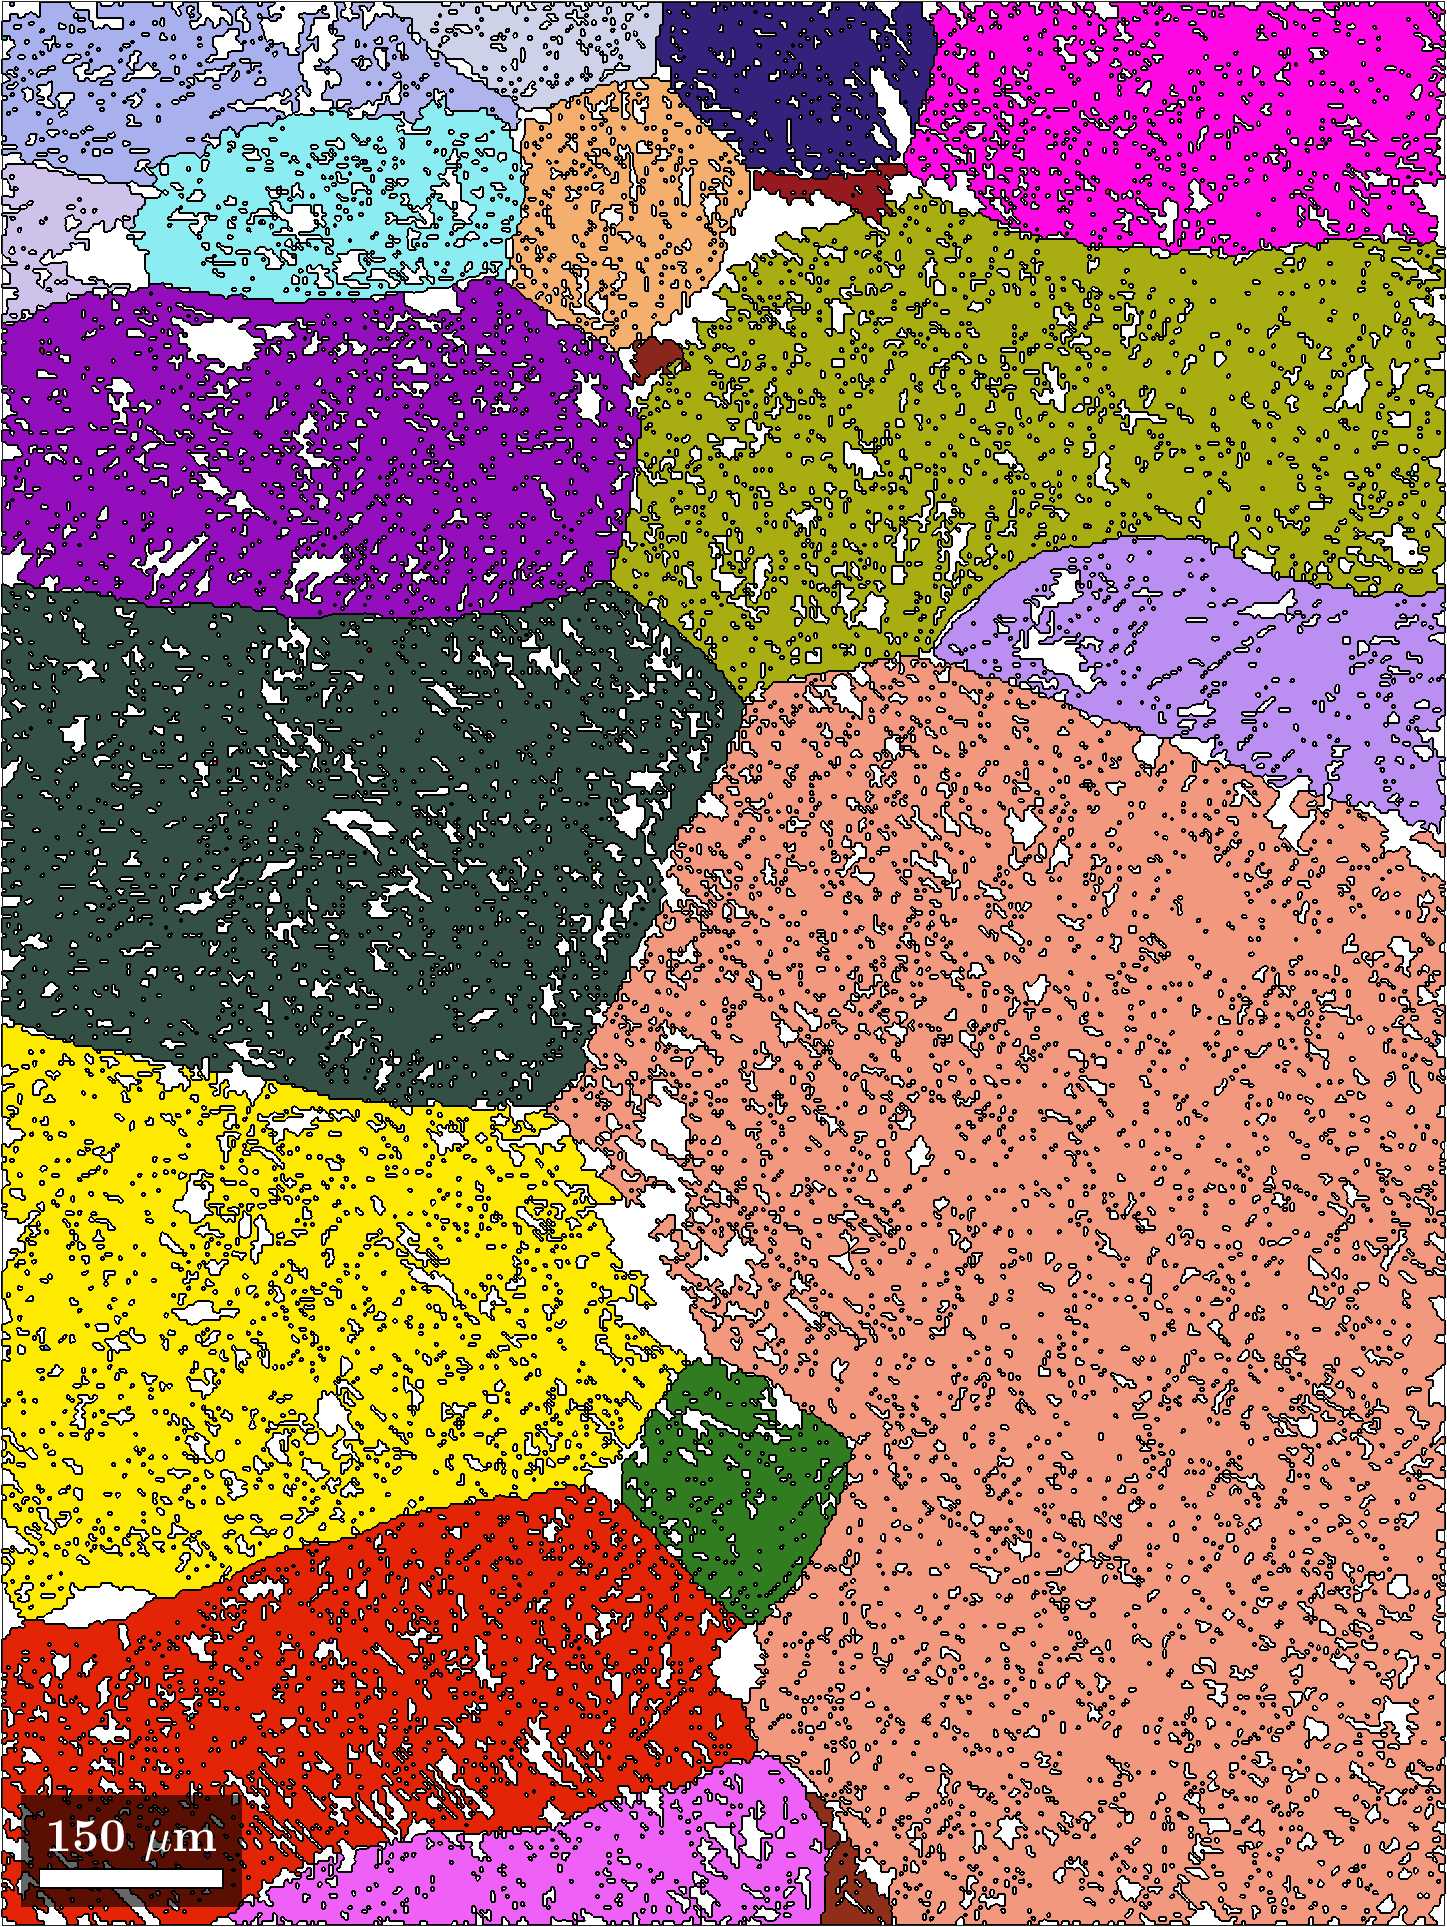
\includegraphics[width=\textwidth]{pic/TiParentMerged1}}
        \only<4>{\vspace{-1cm}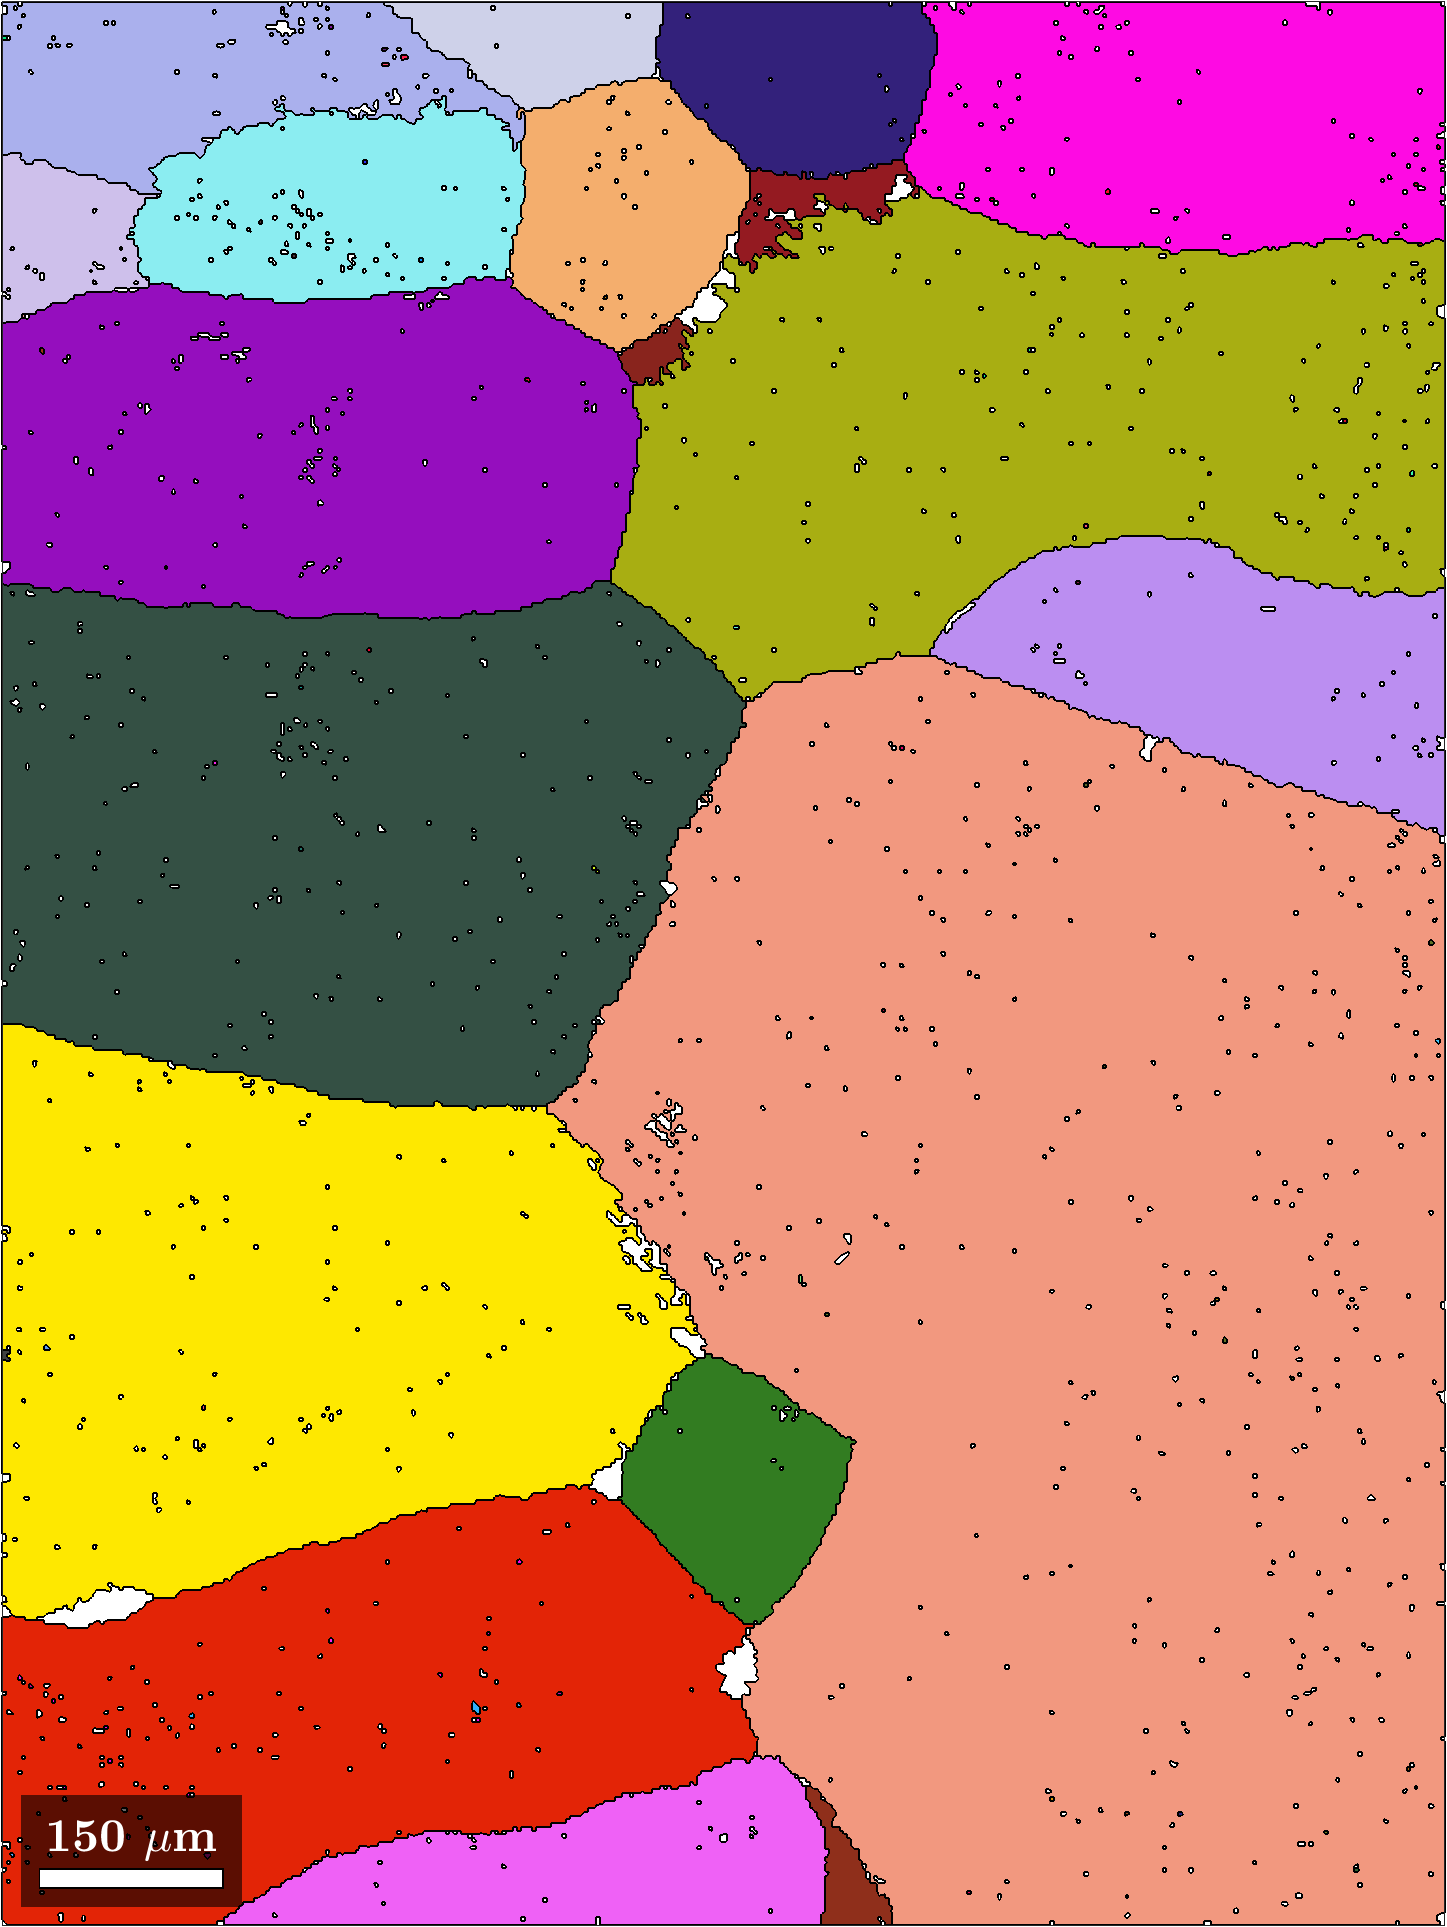
\includegraphics[width=\textwidth]{pic/TiParentMerged2}}
        \only<5>{\vspace{-1cm}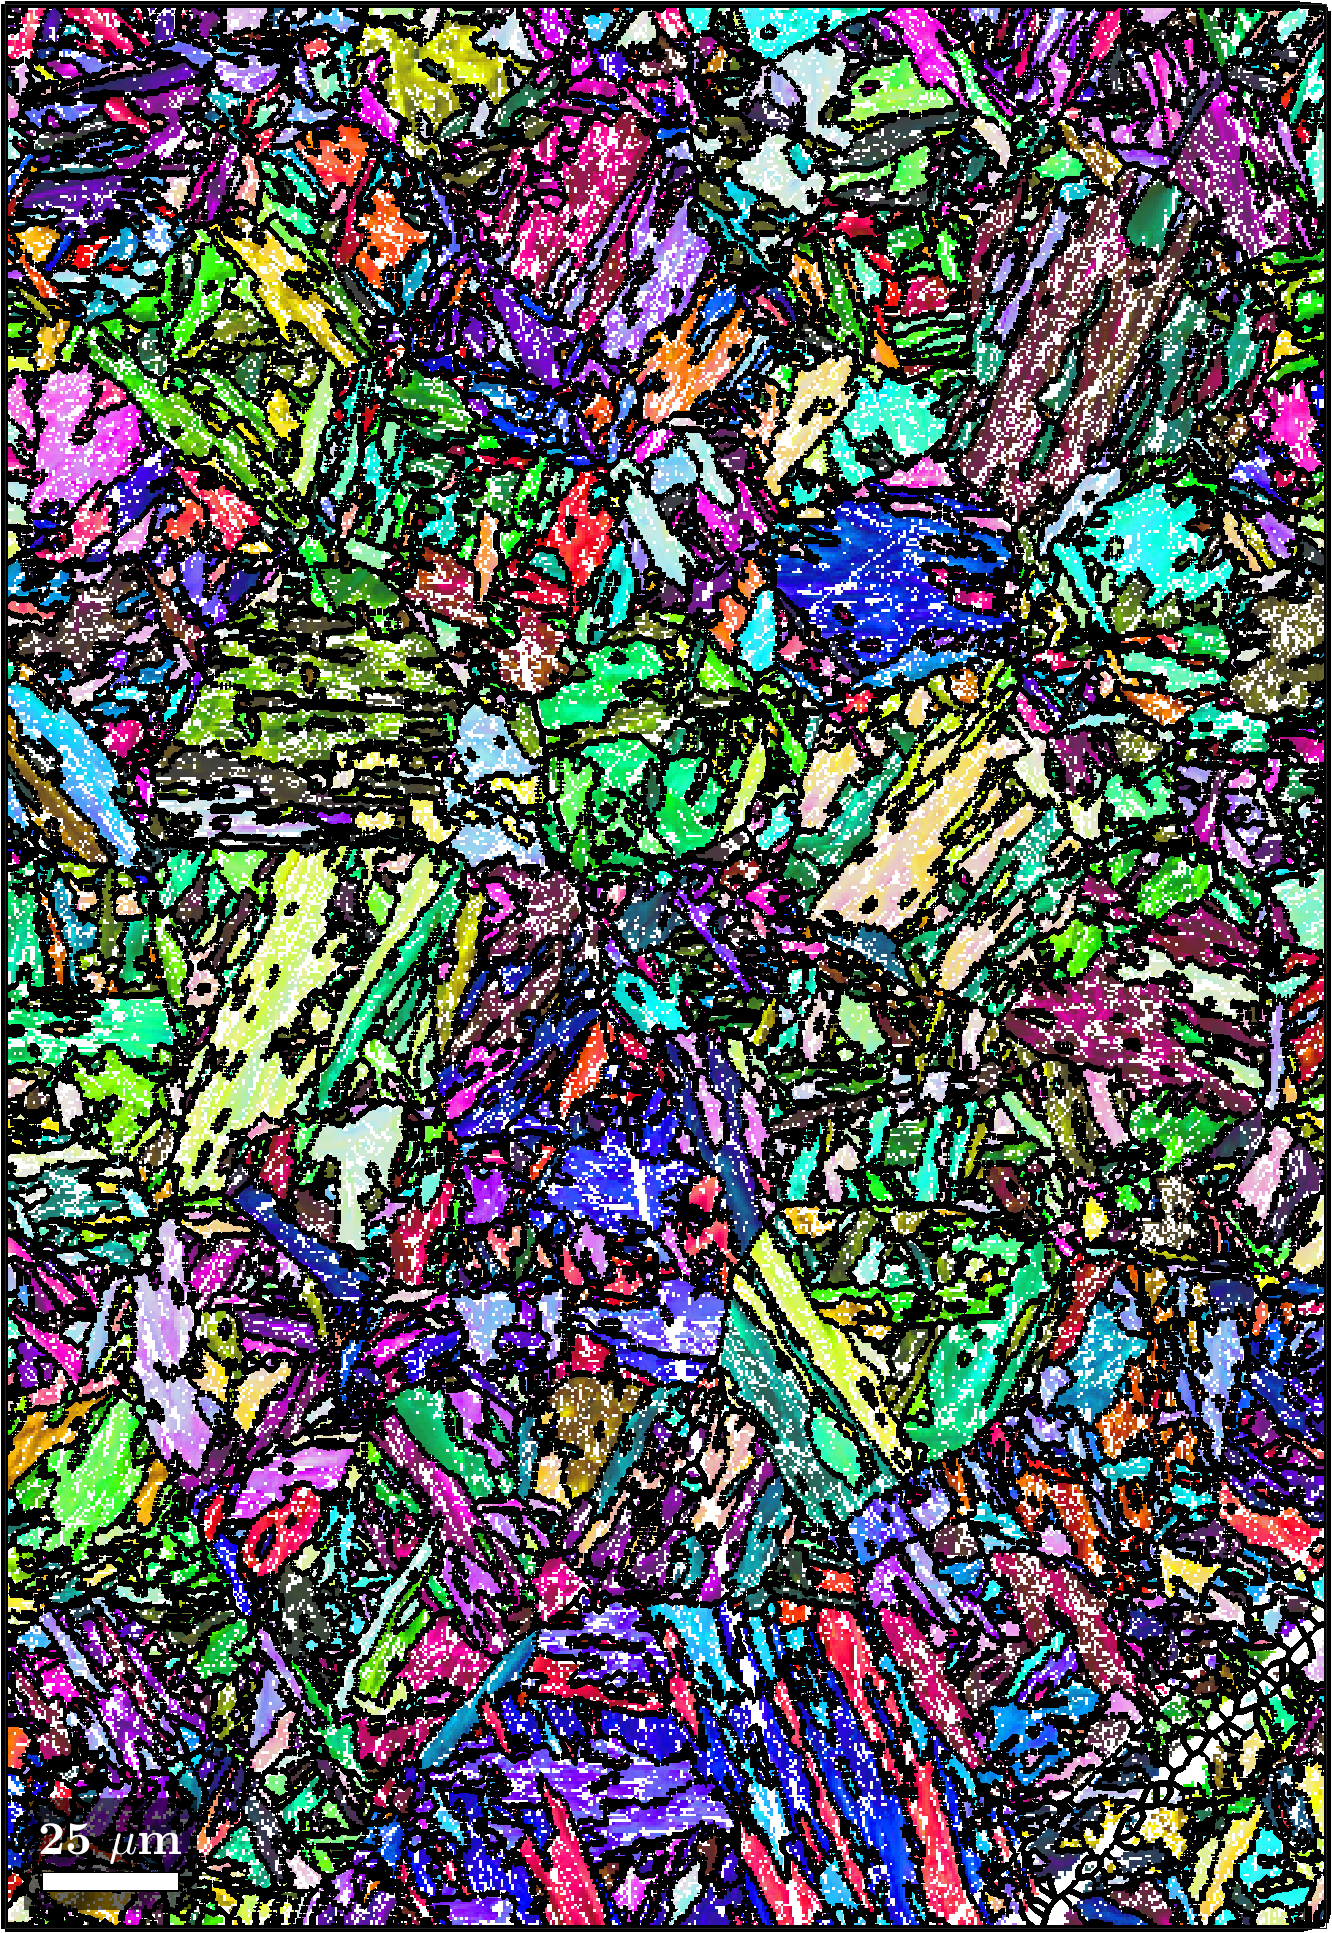
\includegraphics[width=0.94\textwidth]{pic/MaData}}
        \only<6>{\vspace{-1cm}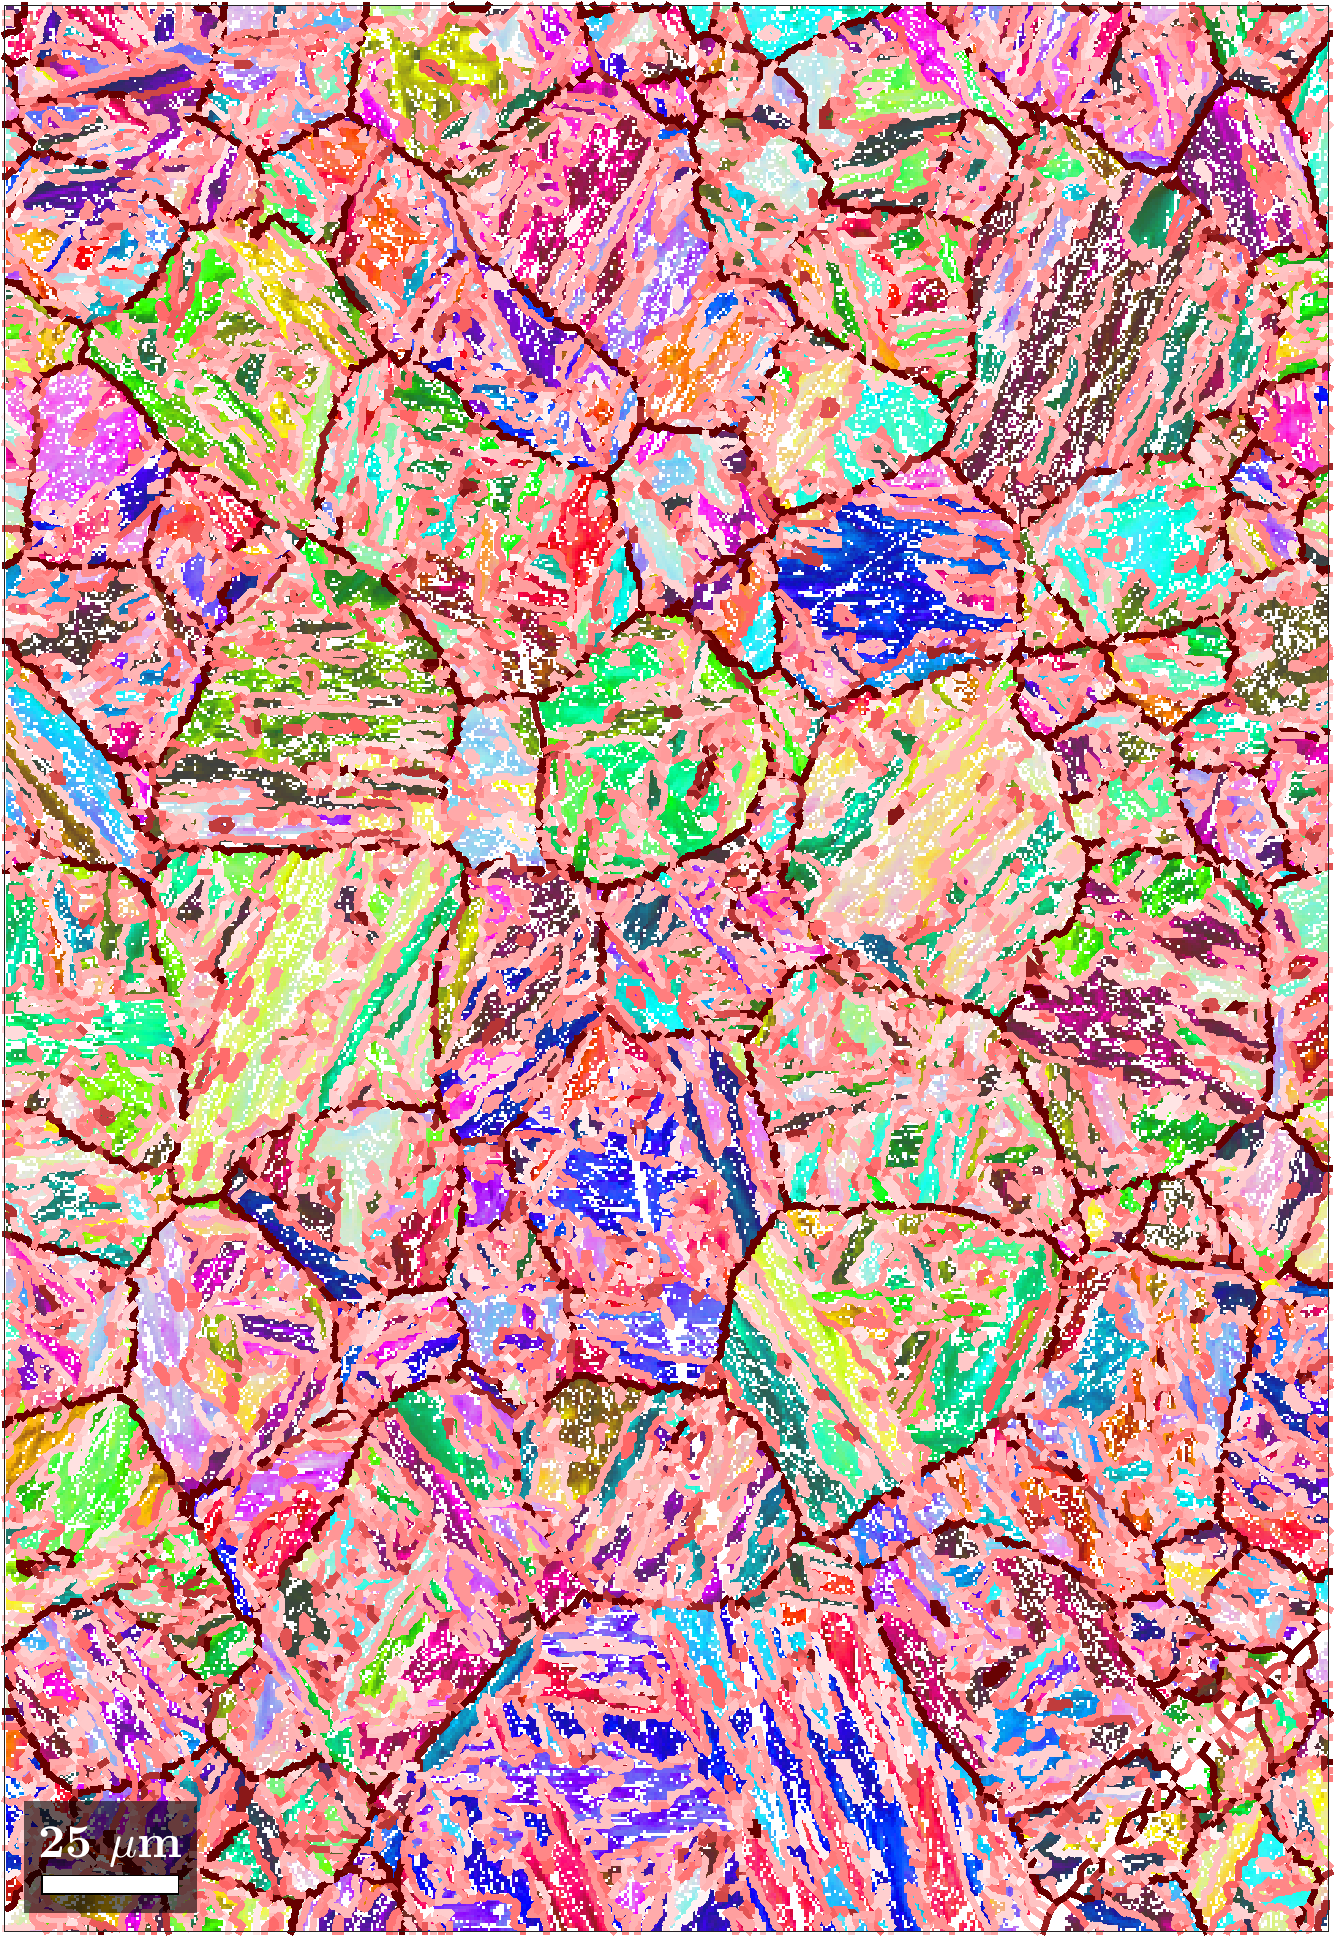
\includegraphics[width=0.94\textwidth]{pic/MaFit2}}
        \only<7>{\vspace{-1cm}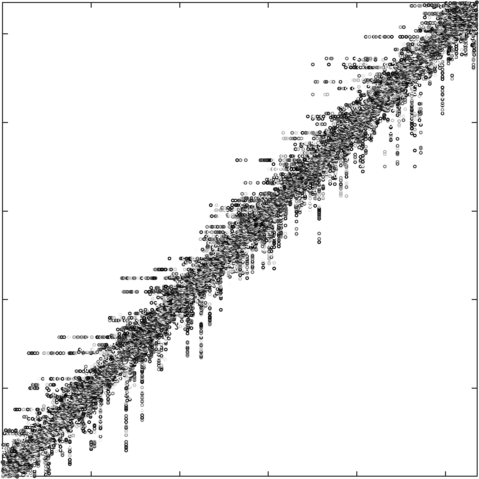
\includegraphics[width=0.94\textwidth]{pic/A}}
        \only<8>{\vspace{-1cm}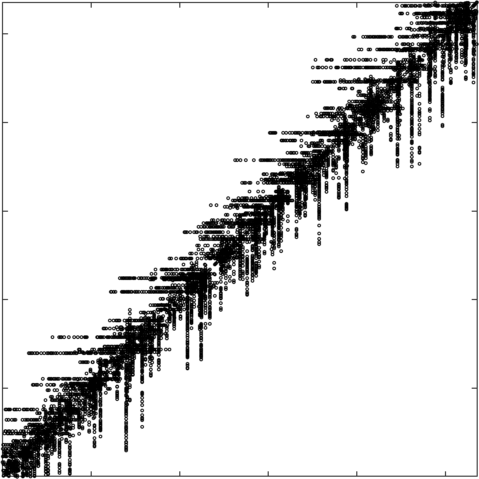
\includegraphics[width=0.94\textwidth]{pic/AA}}
        \only<9>{\vspace{-1cm}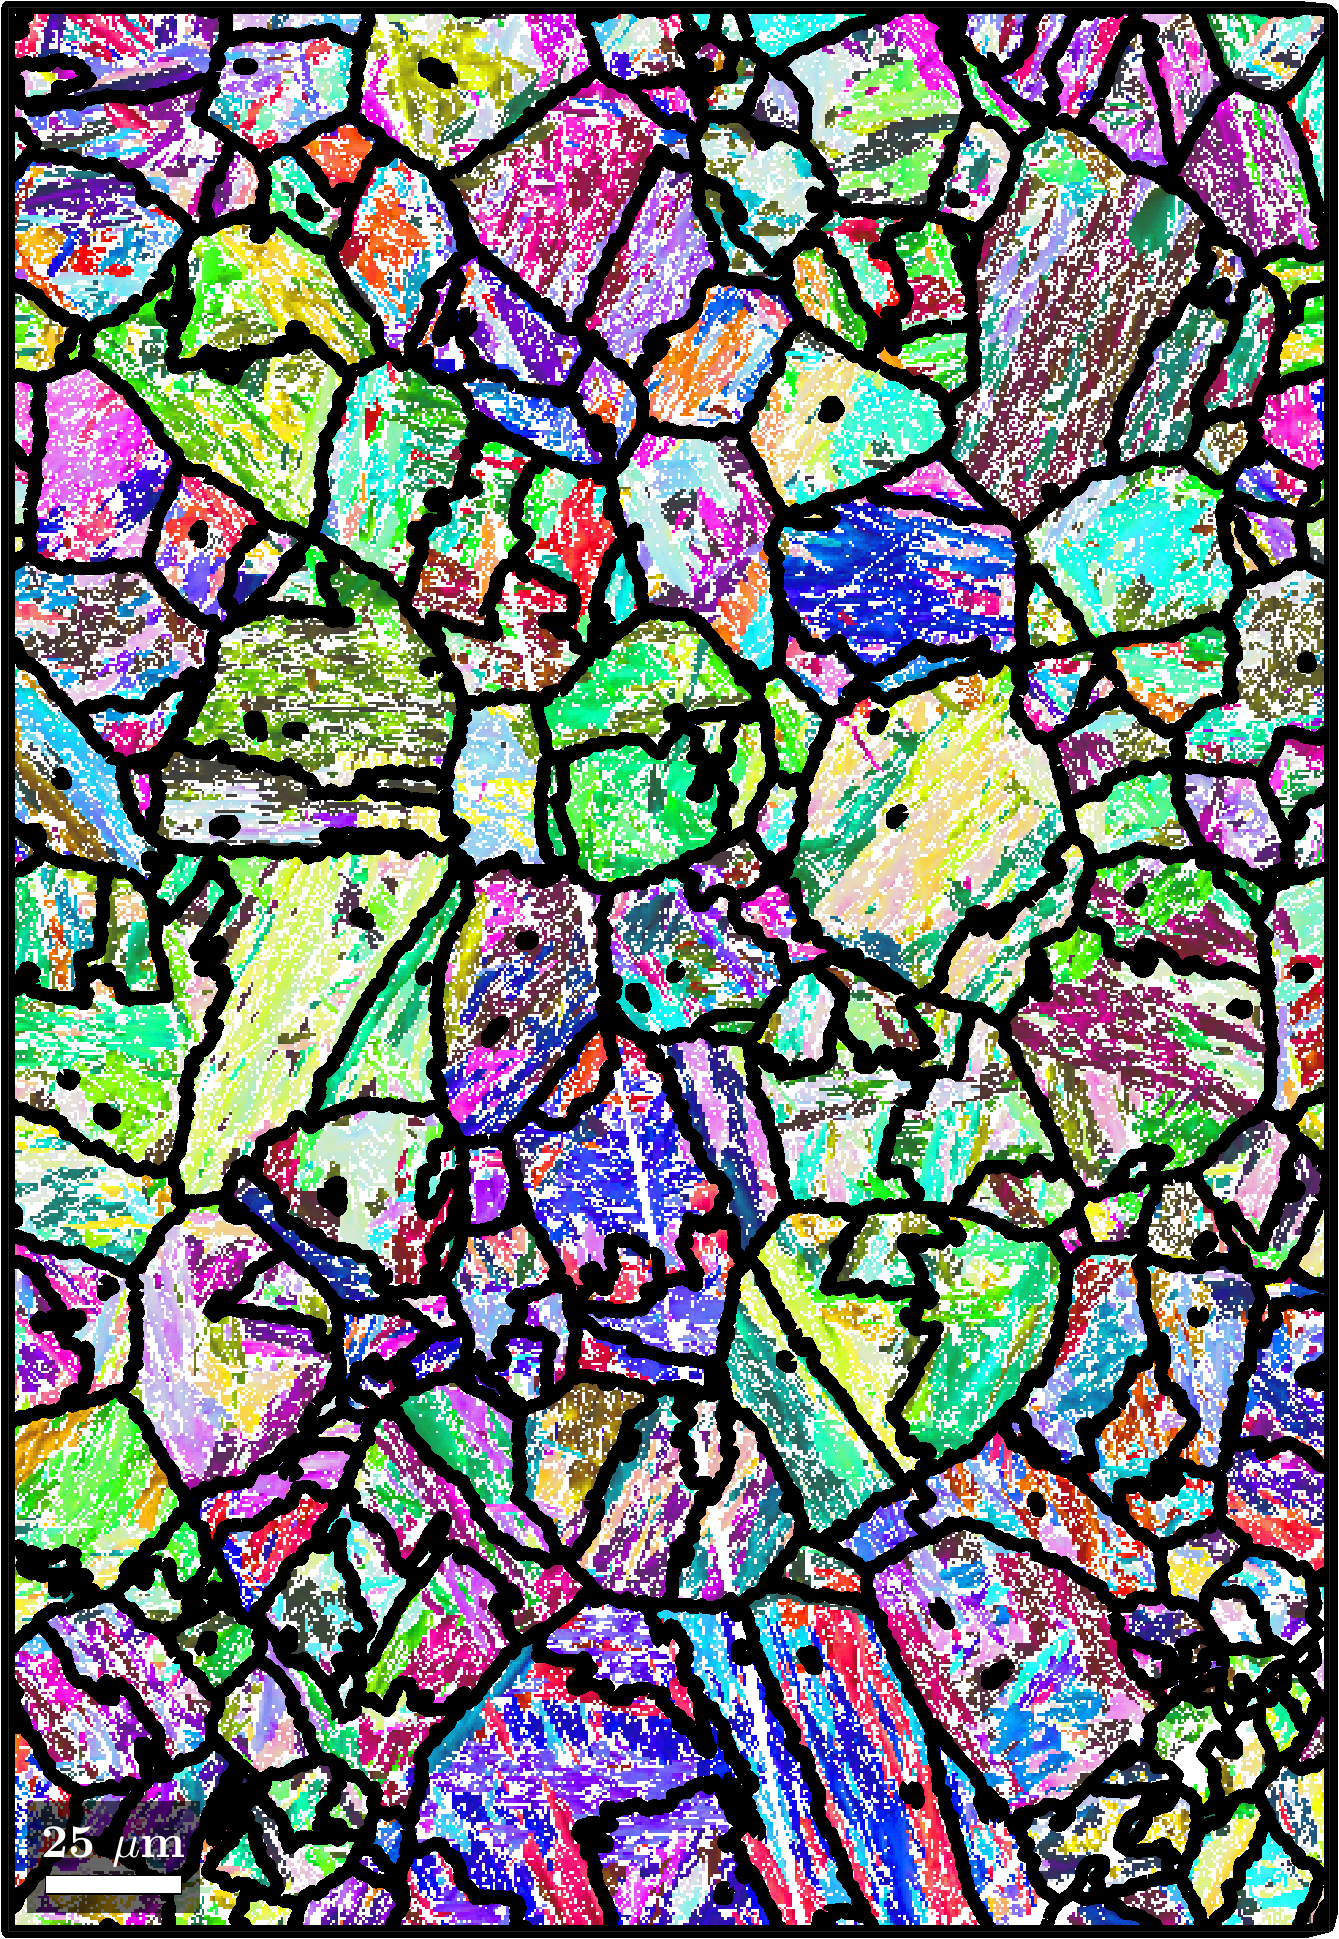
\includegraphics[width=0.94\textwidth]{pic/grainRec}}
        \only<10->{\vspace{-1cm}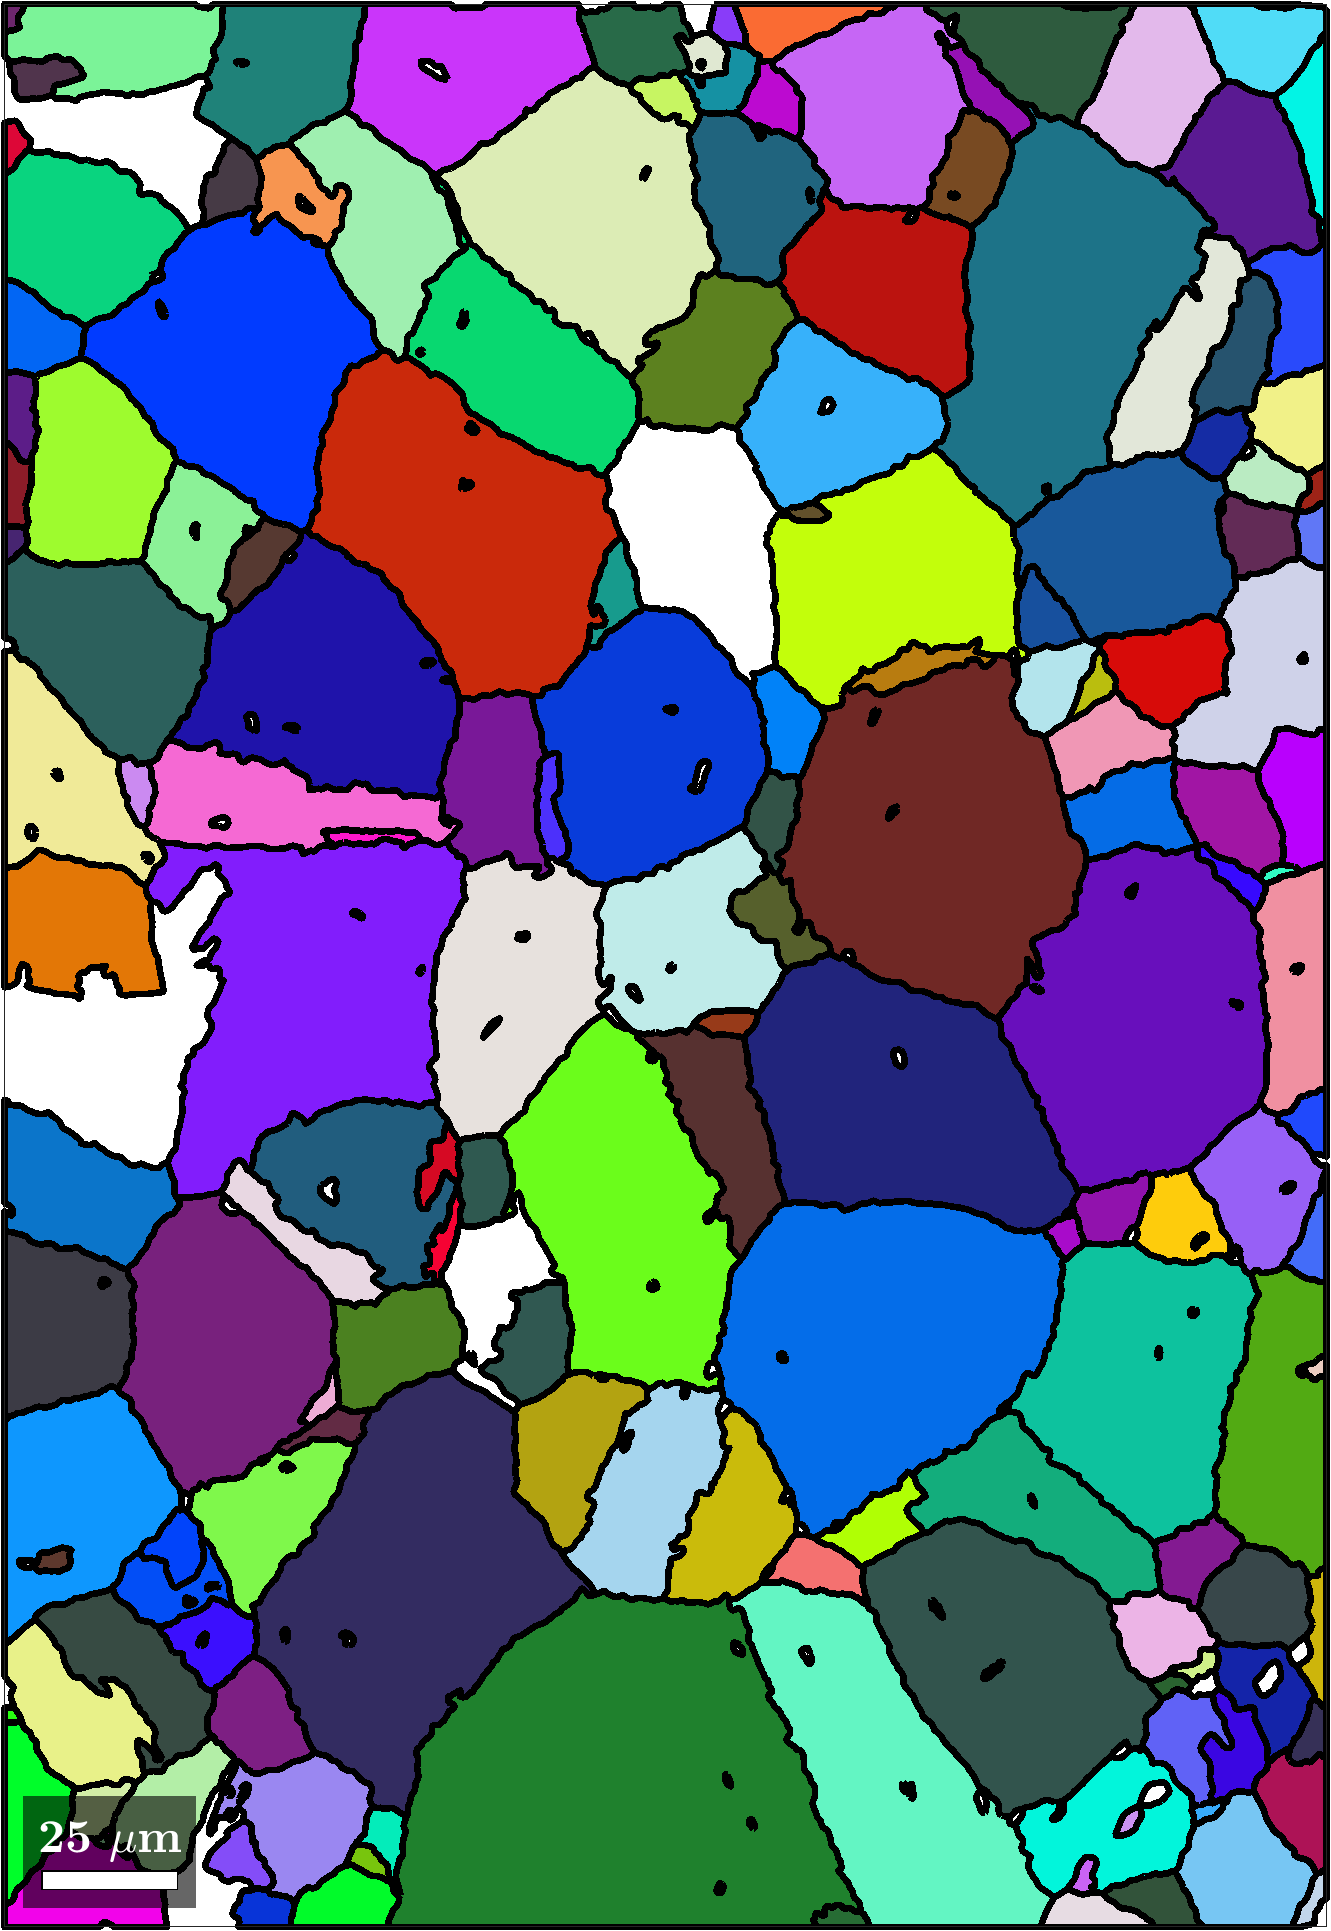
\includegraphics[width=0.94\textwidth]{pic/MaFinal}}
      \end{overlayarea}
    \end{column}
  \end{columns}
\end{frame}


\begin{frame}
  \frametitle{Critical Parameters}

  \begin{block}{orientation first - grain second}
    \begin{itemize}
    \item grain segmentation: threshold $1.5^\circ$
    \item child / child boundaries / triple junctions: threshold $2.5^\circ$
    \item second best fit: lower bound $2.5^\circ$
    \item parent orientation: minimum number of consistent votes 2
    \item child / parent merging: misorientation threshold $2.5^{\circ}$
    \item parent / parent merging: misorientation threshold $2.5^{\circ}$
    \end{itemize}
  \end{block}

  \begin{block}{grain first - orientation second}
    \begin{itemize}
    \item initial grain segmentation threshold $3^\circ$
    \item clustering:\\
      \hspace{0.4cm} method: Markovian clustering algorithm\\
      \hspace{0.4cm} threshold: $2^{\circ}$\\
      \hspace{0.4cm} tolerance: $1.5^{\circ}$\\
      \hspace{0.4cm} inflation power: $p = 1.6$
    \item grain merging: maximum misfit $5^{\circ}$, minimum number of childs
    \end{itemize}
  \end{block}

\end{frame}


\begin{frame}[fragile,fragile,fragile]
    \frametitle{Important Commands}

    parent orientation computation
\begin{lstlisting}[style=input]
[ParentOri, fit] = calcParent(childOri, p2c)
[ParentOri, fit] = calcParent(childOri, p2c, 'numFit', 2)
[ParentOri, fit] = calcParent(childOri, parentOri, p2c)
\end{lstlisting}

\bigskip

    grain merging
\begin{lstlisting}[style=input]
[grainsMerged, childId] = merge(grains, gB)
[grainsMerged, childId] = merge(grains, tP)
[grainsMerged, childId] = merge(grains, M)
[grainsMerged, childId] = merge(grains, 'threshold',delta)
[grainsMerged, childId] = merge(grains, 'inclusions')
\end{lstlisting}

\bigskip

    variant computation
\begin{lstlisting}[style=input]
[variantId, packetId] = calcVariant(parentOri, childOri, p2c)
\end{lstlisting}

  \end{frame}

  \begin{frame}
    \begin{center}
      \centering{\Huge Thank You for Your Attention!}
    \end{center}

    \vspace{1cm}

    \begin{center}
      More information, scripts, data at \\ \medskip \url{mtex-toolbox.github.io/}
    \end{center}

    \vspace{1cm}

    % \begin{center}
    %   MTEX Workshop 2021 - online, in February
    % \end{center}


  \end{frame}

\end{document}
